\documentclass{article}
\usepackage[utf8]{inputenc}
\usepackage{amsmath}
%\usepackage[norsk]{babel}
\usepackage{amssymb}
\usepackage{tikz}
\usetikzlibrary{decorations.markings}
\usepackage{pgfplots}
\usepgfplotslibrary{fillbetween}
\usetikzlibrary{decorations.pathreplacing}
\usetikzlibrary{decorations.pathmorphing}
\usetikzlibrary{calc}
\usepackage{empheq}
\usepackage{amsthm}
\usepackage{xcolor}
\usepackage{physics}
\usepackage{fancyhdr}
\pagestyle{fancy}
\usepackage{esdiff}
\usepackage{tikz-feynman}
\usepackage{hyperref}
\usepackage{mathtools}
\usepackage{cleveref}
\usepackage{ulem}
\usepackage{chngcntr}
\usepackage{graphicx}
\usepackage{subcaption}
\usepackage{enumerate}



\title{Lecture notes FY8305}

\date{August, 2019}


\theoremstyle{definition}
\newtheorem{exmp}{Example}[section]

\counterwithin{equation}{section}

\newcommand{\e}{\mathrm{e}}
\newcommand{\dx}{\dd{x}}
\newcommand{\dy}{\dd{y}}
\newcommand{\dxi}{\dd{\xi}}
\newcommand{\dxis}{\dd{\xi^*}}
\newcommand{\Ha}{\mathcal{H}}
\newcommand{\Z}{\mathcal{Z}}
\newcommand{\normord}[1]{:\mathrel{#1}:}
\newcommand{\D}{\mathcal{D}}
\newcommand{\Sa}{\mathcal{S}}
\newcommand{\J}{\mathcal{J}}
\newcommand{\ad}{a^{\dagger}}
\newcommand{\bd}{b^{\dagger}}
\newcommand{\pd}{\varphi_\downarrow} 
\newcommand{\pu}{\varphi_\uparrow}
\newcommand{\nd}{n_\downarrow} 
\newcommand{\nuu}{n_\uparrow}
\newcommand{\ep}{\varepsilon}
\newcommand{\Gre}{\mathcal{G}_0}
\newcommand{\gre}{\mathcal{G}}

\newcommand{\p}{\varphi}
\newcommand{\pdag}{\varphi^{\dagger}}
\newcommand{\cd}{c^{\dagger}}
\newcommand{\sign}{\text{sign}}
\newcommand{\s}{\Sigma}
\newcommand{\Fd}{F^{\dagger}}
\newcommand{\fd}{f^{\dagger}}


\tikzset{->-/.style={decoration={
  markings,
  mark=at position #1 with {\arrow{>}}},postaction={decorate}}}

\tikzset{snake it/.style={decorate, decoration=snake, mark=at position #1 with {\arrow{>}}}, ,postaction={decorate}}

\newcommand{\contribs}{%
\begin{center}
\Large 
\textbf{Contributors}
\end{center}


\begin{itemize}
\item Karl Kristian Ladegård Lockert
\item Snorre Bergan
\end{itemize}

%\clearpage
}



\begin{document}

\maketitle
Digitialized lecture notes for the course ``FY8305 - Functional Integral Methods in Condensed Matter Physics''.

These notes follow the pdf containing the hand written lecture notes for the course ``FAG 74986 Funksjonal-integral metoder HØST 1996''.
Website: \href{https://www.ntnu.edu/studies/courses/FY8305}{https://www.ntnu.edu/studies/courses/FY8305}
\contribs
\tableofcontents

\section{Uncertainties/mistakes}

\begin{itemize}
\item Something weird in the derivation of \eqref{unc:statmech}.
\item The indices in equation \eqref{unc:indices} seems off.  
\item In the proof in section \ref{unc:proof} i think there should be a creation operator on one of the last lines in the proof, not annihilation operator as it stands in the notes. $a\e^{\varphi a^\dagger}\ket{0}$ instead of $a\e^{\varphi a}\ket{0}$
\item It is a somewhat unclear purpose of ~\Crefrange{unc:expvalN}{unc:expvalN2}. 
\item The ordering of headlines and equations in section \ref{unc:order_boson} is a bit weird, and some things seem a bit unmotivated. 
\item Double check the labeling on states/ sub indices in \eqref{unc:labeling_on_states} and the previous few eqs. 

\end{itemize}
\section{Short recap of second quantization for fermions and bosons}
Pages 2-10 in lecture notes.

Notation: $ \mu = $ set of quantum numbers that define a one-particle state.


\subsection{Many particle basis}
\newtheorem{theorem}{Ex}
\begin{theorem}


\begin{align*}
\mu &= (\vec{k}, \sigma):\text{Wave number, spin} \\
\mu &= (i, \sigma) : \text{Lattice point, spin} \\
\mu &= (n, i) : \text{Orbital, lattice point} \\
\end{align*}

\end{theorem}

A many-particle basis can be written $\ket{\phi} = \ket{n_{\mu}, n_{\nu}, \dots, n_{\mu_N}}$. Many particle states are built by combining many one-particle states, but where the one-particle states are not necessarily independent. If  \underline{one} of the set of quantum numbers, $\mu_i$, are changed, this \underline{scattering} will generally have consequences for the distribution of quantum numbers for the remaining sets $\{\mu_j\}_{j\ne i}$.
We generally imagine that many-particle states can be built as a linear combination of
$\ket{\phi}$'s;
\begin{equation}
\ket{\Psi} = \sum_{n_{\mu_1},\dots, n_{\mu_N}}\phi_{{\mu_1},\dots, n_{\mu_N}}\ket{{\mu_1},\dots, n_{\mu_N}}.
\end{equation}
A definite one-state vector $\ket{n_{\mu},\dots, n_{\mu_N}}$ can be demanded from a vacuum state (where there is no filled one-particle states) $\ket{0}$ via creation operators.
\begin{align*}
&\textbf{bosons}: &a_\mu^\dagger \\ 
&\textbf{fermions}: &c_\mu^\dagger
\end{align*}


A quanta in a one-particle state can be destroyed by the annihilation operators.

\begin{align*}
&\textbf{bosons}: &a_\mu \\ 
&\textbf{fermions}: &c_\mu
\end{align*}


These operators satisfy some commutation relations:
\begin{align}
&[a_\mu, a_{\nu}] & = [a_\mu^\dagger, a_{\nu}^\dagger] = 0 \\
&[a_\mu, a_{\nu}^\dagger] & = \delta_{\mu\,\nu} \\
&[A,B] &= AB-BA \\
&\{c_\mu^\dagger, c_{\nu}^\dagger\} & = \{c_\mu, c_{\nu}\} = 0 \\
&\{c_\mu, c_{\nu}^\dagger\} & = \delta_{\mu\,\nu} \\
&\{A,B\} &= AB + BA
\end{align}
These will automatically satisfy the Pauli principle as well, which gives \emph{symmetri/ \emph{antisymmetric}} solutions by exchange, dependent if the particles are bosons/fermions. 


\subsection{From classical formulation to second quantization of one-particle operators}

For one-particle operators we usually have a kinetic energy function on a form like
\begin{equation}
T = \sum_i T\left(\vec{r}_i, \vec{p}_i\right) = \sum_i T\left(\vec{r}_i, \diffp{}{r}\right)
\end{equation}
\begin{theorem}
External electrostatic potential:
\begin{equation}
T = \sum_i V_{\text{ext}}\left(\vec{r}_i\right)
\end{equation}
\end{theorem}
\begin{theorem}

Kinetic energy:

\begin{equation}
T = \sum_i \frac{p^2}{2m} = -\sum_i \frac{\hbar^2}{2m}\nabla_i^2
\end{equation}
\end{theorem}

\begin{theorem}
Crystal-potential:
\begin{equation}
T = \sum_i \sum_j v_{\text{cryst}} \left( \vec{r}_i, \vec{R}_j \right)
\end{equation}
\end{theorem}

Second quantization by an operator on this form can be written 
\begin{equation}
T = \sum_{\mu, \nu} T_{\mu\nu}c_\mu^\dagger c_{\nu},
\end{equation}
where
\begin{equation}
T_{\mu\,\nu} = \mel{\mu}{T\left(\vec{r}, \vec{p}\right)}{\nu}.	
\end{equation}

\textbf{Note: The matrix element of one-particle operators are determined by matrix elements in the Hilbert space of one-particle states.}

\subsection{From classical formulation to second quantization of two-particle operators}

Typically, we consider pair-potentials 
\begin{equation}
V = \sum_{i, j} V\left(\vec{r}_i, \vec{r}_j\right).
\end{equation}

\begin{theorem}
Exchange interaction of two charges
\begin{equation}
V = \frac{e^2}{2}\sum_{i\ne j} \frac{1}{|\vec{r}_i - \vec{r}_j|}
\end{equation}
\end{theorem}

The second quantization versions of these are

\begin{equation}
V = \sum_{\mu, \dots, \beta} V_{\mu\nu\alpha\beta}c_{\mu}^\dagger c_{\nu}^\dagger c_{\alpha}c_{\beta},
\end{equation}
where again
\begin{equation}
V_{\mu\nu\alpha\beta} = \mel{\mu\nu}{V\left(\vec{r}_i, \vec{r}_j\right)}{\beta\alpha}
\end{equation}

\textbf{Note: The matrix element of two-particle operators are determined by matrix elements in the Hilbert room of two-particle states.}

The Hamiltonian:
\begin{align}
H &= T + V \label{eq:hamiltonian} \\
T &= -\sum_i \frac{\hbar^2}{2m}\nabla_i^2
\end{align}
So far, we have just presented second quantization for fermion operators, but an equivalent statement will of course hold for the second quantization version of the Hamiltonian for an interacting, material, bosonic system, which has the same identical form as \eqref{eq:hamiltonian}. Notice that each term in $H$ has just as many $c_\mu^\dagger$ as $c_{\nu}$.


\begin{figure}
\centering
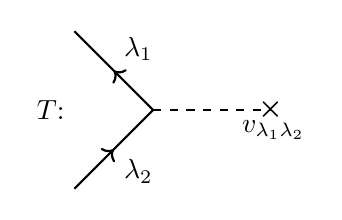
\begin{tikzpicture}

	\draw[thick, ->- = 0.5] (0,0) -- (1,1);
	\draw[thick, ->- = 0.5] (1, 1) -- (0,2);
	\draw[thick, dashed] (1, 1) -- (2.5, 1);
	\node[thick] at (2.5,1){$\cross$};
	\node[anchor = north west, thick] at (0.5, 0.5) {$\lambda_2$};
	\node[anchor = south west, thick] at (0.5, 1.5) {$\lambda_1$};
	\node[anchor = north west, thick] at (2, 1) {$v_{\lambda_1\lambda_2}$};
	\node[anchor = east] at (0, 1) {$T$:};
\end{tikzpicture}
\caption{Scattering from an external potential $v_{\mu\nu}c_{\mu}^\dagger c_{\nu}$}
\end{figure}


\begin{figure}
\centering
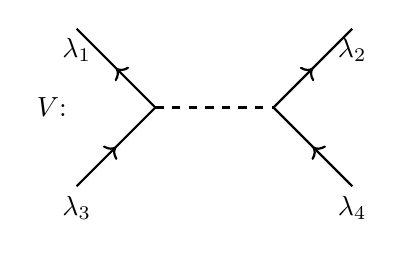
\begin{tikzpicture}

	\draw[thick, ->- = 0.5] (0,0) -- (1,1);
	\draw[thick, ->- = 0.5] (1, 1) -- (0,2);
	\draw[thick, dashed] (1, 1) -- (2.5, 1);
	\draw[thick, ->- = 0.5] (3.5, 0) -- (2.5, 1);
	\draw[thick, ->- = 0.5] (2.5, 1) -- (3.5, 2);
	
	\node[anchor = north] at (0, 0){$\lambda_3$};
	
	\node[anchor = north] at (0, 2){$\lambda_1$};	
	
	\node[anchor = north] at (3.5, 0){$\lambda_4$};

	\node[anchor = north] at (3.5, 2){$\lambda_2$};
	
	\node[anchor = east] at (0, 1) {$V$:};
\end{tikzpicture}
\caption{Exchange interaction between two particles.}
\end{figure}


\subsection{Statistical mechanics}

Assume that we know the spectrum $E_N^n$ for an interacting many-particle system, defined by a state $\ket{\psi_N}_n$, where $N$ is the number of particles in the system and $n$ is an index that indicates what excited state $\ket{\psi_N}_n$ the system is in. 
$\ket{\psi_N}$ is also assumed to be known, such that the matrix product of observables can be calculated: 
\begin{equation}
H\ket{\psi}_n = E_N\ket{\psi}_n.
\end{equation}

To do statistical mechanics, we need to introduce temperature. We do this by using the canonical partition function
\begin{equation}
\label{eq:partition_function}
Z_N = \sum_n\e^{-\beta E_N^n}.
\end{equation}

Note, in \eqref{eq:partition_function} we sum over states, \underline{not} the energy levels $E_N^n$.

\begin{align}
Z &= \sum_n {}_n\mel{\psi_N}{\e^{-\beta H}}{\psi_N}_n \nonumber \\
 &= \Tr\left(\e^{-\beta H}\right) = \Tr\left(S^{-1}S\e^{-\beta H}\right) \nonumber\\
 &= \Tr\left(S\e^{-\beta H}S^{-1}\right) \nonumber \\
 &= \sum_{n'}{}_{n'}\mel{\phi_N}{\e^{-\beta H}}{\phi_N}_{n'}. \label{eq:basis_invariant}
\end{align}

We see in \eqref{eq:basis_invariant} that we can use an \underline{arbitrary} basis to calculate the partition function. The most convenient basis is often a basis where the Hamiltonian is diagonal, but not always.

We write the statistical mean value of an operator as
\begin{align}
\expval{\hat{O}} &\equiv \frac{1}{Z}\Tr\left(\hat{O}\e^{-\beta H}\right) \nonumber\\
&= \frac{1}{Z} \sum_n {}_n\mel{\psi_N}{\hat{O}\e^{-\beta H}}{\psi_N}_n \nonumber \\
&= \frac{1}{Z} \sum_{n, n'} {}_n\expval{\hat{O}}{\psi_N}_{n'}\underbrace{{}_{n'}\expval{\e^{-\beta H}}{\psi_N}_n}_{\delta_{nn'}\e^{-\beta E_{n'}}}.
\end{align}
Thus, we have 
\begin{equation}
\label{eq:expval}
\expval{\hat{O}} = \frac{1}{Z}\sum_n \underbrace{{}_n\expval{\hat{O}}{\psi_N}_n}_{\text{QM matrix element}}\e^{-\beta E_N^n}.
\end{equation}
Notice how the temperature, $T$ only appears in the last factor in \eqref{eq:expval}.
Let us now consider the ground state ($n = 0$) in the low temperature limit with energy $E_0$ corresponding to the state $\ket{\psi_N}_0$.
\begin{align*}
\expval{\hat{O}} &\simeq \frac{1}{Z_{\beta = \infty}}\e^{-\beta E_0} {}_0\expval{\hat{O}}{\psi_N}_0 \\
&= \frac{\e^{-\beta E_0}}{\e^{-\beta E_0}}{}_0\expval{\hat{O}}{\psi_N}_0, 
\end{align*}

such that 
\begin{equation}
\expval{\hat{O}} \stackrel{\beta \rightarrow \infty}{=} {}_0\expval{\hat{O}}{\psi_N}_0.
\end{equation}

We now have a way to calculate the statistical mean value in the ground state at zero temperature. Let us now now assume that the energy spectrum is such that the ground state is separated from excited states by a  \underline{gap} (band insulators, semiconductors, superconductors). This way, we can express the excited state energies as 

\begin{equation}
E_N^1 = E_N^0 + \Delta_N
\end{equation}

such that 
\begin{equation}
E_N^2, E_N^3, \dots \ge E_N^1. 
\end{equation}

This way, we get from \eqref{eq:expval}

\begin{align}
\expval{\hat{O}} &= \frac{1}{Z}\sum_n {}_n\expval{\hat{O}}{\psi_N}_n\e^{-\beta E_N^n} \nonumber\\
&= \frac{\sum_n {}_n\expval{\hat{O}}{\psi_N}_n\e^{-\beta E_N^n}}{\sum_n\e^{-\beta E_N^n}} \nonumber\\
&= \cdots \nonumber\\
% Something fishy right here
&= \frac{{}_0\expval{\hat{O}}{\psi_N}_0\e^{-\beta E_N^0\left(1+\e^{-\beta\Delta}\dots\right)}}{\e^{-\beta E_N^0}\left(1+\e^{-\beta\Delta}\dots\right)} \label{unc:statmech}
\end{align}
and we find that as $\beta\Delta >> 1$, $\hat{O} \simeq {}_0\expval{\hat{O}}{\psi_N}_0$.
In semiconductors we find $\Delta \sim 10\mathrm{mev} \sim 1000\mathrm{K}$.






















\section{Coherent states and Grassman variables}
Pages 10-17 in lecture notes.

\subsection{Coherent states}
A coherent state (both for fermions and bosons) is defined as an eigenstate to an annihilation operator

\begin{align}
	a_\mu \ket{\phi} &= \varphi_\mu \ket{\phi} & \textbf{Bosons}\\
	c_\mu \ket{\psi} &= \xi_\mu\ket{\psi} & \textbf{Fermions}
\end{align}

Both $\ket{\psi}$ and $\ket{\phi}$ must contain a component with the least ($\ge 0$) quantum number (quant), but it is clear that neither $\ket{\psi}$ nor $\ket{\phi}$ can be states with a sharply defined number of particles. They are therefore also ``hard to destroy''. This also explains why we chose to define them as eigenstates of the annihilation operators, not the creation operators. We will get back to the creation of these coherent states. 

We will first look at the bosonic case:
\subsubsection{Bosonic case}

\begin{equation}
a_\mu\ket{\phi} = \varphi_\mu\ket{\phi}
\end{equation}

\begin{align}
[a_\mu, a_{\nu}] = 0& &\nonumber \\
 &\Rightarrow \left(a_\mu a_{\nu} -a_{\nu}a_\mu\right)\ket{\phi} = 0 & \nonumber \\
&= \left(\varphi_\mu\varphi_{\nu} - \varphi_{\nu}\varphi_\mu\right)\ket{\phi} &\nonumber\\
&&\Rightarrow [\varphi_\mu, \varphi_\nu] = 0. \label{eq:coherent_commutator} 
\end{align}

Equation \eqref{eq:coherent_commutator} will always be satisfied if $\varphi_\mu \in \mathbb{C}$. \textbf{The eigenvalues to coherent boson states can be chosen as complex numbers. This is something we can state without knowing anything about how these states are constructed. }

\subsubsection{Fermionic case}
\begin{align}
\{c_\mu, c_\nu\} = 0 && \nonumber \\
&\left(c_\mu c_\nu + c_\nu c_\mu\right)\ket{\psi} = 0 &\nonumber \\
&=\left(\xi_\mu\xi_\nu + \xi_\nu\xi_\mu\right)\ket{\psi} &\nonumber \\
&&\Rightarrow \{\xi_\mu,\xi_\nu\} = 0.\label{eq:coherent_anticommutator}
\end{align}

If $\xi_\mu\in\mathbb{C}$, \eqref{eq:coherent_anticommutator} will only be satisfied if $\{\xi_\mu\} = 0$, trivial eigenvalues. \textbf{The eigenvalues for coherent fermion states must be chosen as anti-commuting numbers, Grassmann-variables.}

\subsection{Grassmann variables}
\subsubsection{Fundamentals}

Equation \eqref{eq:coherent_anticommutator} states the fundamental property of Grassmann variables, and it immediately follows that 
\begin{equation}
\xi_\mu^2 = 0,
\end{equation}
the squares of the Grassmann variables vanish!
Similarly we have that $\xi^n = \xi^2\xi^{n-2} = 0, n \ge 2$.
An arbitrary series expansion in Grassmann variables
\begin{align}
f(\xi) &= \sum_nc_n\xi^n \nonumber \\
&=c_0 + c_1\xi + \dots \nonumber\\
&= x_0 + c_1\xi
\end{align}
is linear.
An arbitrary function of $\xi, \xi^*$ can be written on the forms
\begin{align*}
A\left(\xi, \xi^*\right) &= c_0 + c_1\xi + c_2\xi^*+c_3\xi\xi^* \\
&= c_0 + c_1\xi + c_2\xi^*+d_3\xi^*\xi
\end{align*}

\subsubsection{Grassmann algebra}
We will now look into some of the propreties of functions of Grassmann variable. 

\section{Construction of coherent states for bosons, and its properties}

Pages 18-26 in lecture notes.

\subsection{Construction}
The definition of a coherent boson state $\ket{\phi}$ is stated in \eqref{eq:def_boson_coherent_state}. We make an ansatz -- a qualified guess -- that $\ket{\phi}$ can be created as
\begin{equation}
\label{eq:construction_coherent_boson}
\ket{\phi} = \e^{\sum_\mu\varphi_\mu a_\mu^\dagger}\ket{0}.
\end{equation}

We claim that 
\begin{equation}
\label{unc:indices}
a_\mu\e^{\sum_\nu\varphi_\nu a_\nu^\dagger}\ket{0} = \varphi_\mu\e^{\sum_\nu\varphi_\nu a_\nu^\dagger}\ket{0}
\end{equation} % TODO: CHECK THIS

\begin{proof}
\label{unc:proof}
\begin{equation*}
a\sum_{n=0}\frac{\left(\varphi a^\dagger\right)^n}{n!}\ket{0} = a\sum_{n=1} \frac{\varphi^n}{n!}\left(a^\dagger\right)^n\ket{0}.
\end{equation*}
Note that $\left(a^\dagger\right)^na\ket{0} = 0$, and so we wish to ``commute $a$ through''.

\begin{align*}
\comm{a}{f\left(a^\dagger\right)} &= \sum_{n=1}c_n\comm{a}{\left(a^\dagger\right)^n} \\
&= \sum_{n=1}nc_n\left(a^\dagger\right)^{n-1}\\
f\left(a^\dagger\right) &= \sum_{n=0}^\infty c_n\left(a^\dagger\right)^n \\
&\implies \comm{a}{f\left(a^\dagger\right)} = \pdv{a^\dagger}f\left(a^\dagger\right).
\end{align*}

More generally:

\begin{align*}
\comm{g(a)}{f(a^\dagger)} &= g\left(\pdv{a^\dagger}\right)f\left(a^\dagger\right)\\
\comm{a}{\left(a^\dagger\right)^n} &= n\left(a^\dagger\right)^{n-1} \\
\comm{\left(a\right)^m}{\left(a^\dagger\right)^n} &= \frac{n!}{(n-m)!}\left(a^\dagger\right)^{n-m} \\
\acomm{c}{f\left(c^\dagger\right)} &= \pdv{c^\dagger}f\left(c^\dagger\right) \\
\acomm{g(c)}{g(c^\dagger)} &= g\left(\pdv{c^\dagger}\right)f\left(c^\dagger\right)
\end{align*}

To find out what the commutator $\comm{a}{\left(a^\dagger\right)^n}$ is, we use that 
\begin{equation}
\comm{A}{BC} = \comm{A}{B}C + B\comm{A}{C}, 
\end{equation}
with $A =a, B = a^\dagger, C = \left(a^\dagger\right)^{n-1}$ to get

\begin{align*}
\comm{a}{\left(a^\dagger\right)^n} &= \left(a^\dagger\right)^{n-1} + a^\dagger\comm{a}{\left(a^\dagger\right)^{n-1}} \\
&= a\left(a^\dagger\right)^{n-1} \\
\implies a\left(a^\dagger\right)^{n}\ket{0} &= n\left(a^\dagger\right)^{n-1}\ket{0}\\
\implies a\e^{\varphi a^\dagger}\ket{0} &= \sum_{n=1}^\infty\frac{\varphi^nn\left(a^\dagger\right)^{n-1}}{n!}\ket{0} \\
&= \varphi\sum_{n=1}^\infty\frac{\left(\varphi a^\dagger\right)^{n-1}}{(n-1)!}\ket{0}\\ &= \varphi\e^{\varphi a^\dagger}\ket{0}.
\end{align*}
\end{proof}

Then, for more modes (quantum numbers), we get
\begin{equation}
\ket{\phi} = \e^{\sum_\mu\varphi_\mu a_\mu^\dagger}\ket{0}
\end{equation}
with the $\varphi_\mu$'s satisfying
\begin{equation}
a_\mu\ket{\phi} = \varphi_\mu\ket{\phi}.
\end{equation}
Coherent states: ``difficult to destroy''.

We also could have done this in a more direct way:
Assume
\begin{equation}
\ket{\phi} = \prod_\mu f_\mu\left(\varphi, a_\mu^\dagger\right)\ket{0}
\end{equation}
with 
\begin{equation}
a_\mu =\varphi_\mu\ket{\phi}.
\end{equation}

Then, we need that 
\begin{equation}
a_\mu f_\mu\left(\varphi, a_\mu^\dagger\right)\ket{0} = \varphi_\mu f_\mu\left(\varphi, a_\mu^\dagger\right)\ket{0},
\end{equation}

but

\begin{align}
a_\mu f_\mu \ket{0} &= \comm{a_\mu}{f_\mu}\ket{0}\\
&\implies \pdv{a_\mu^\dagger} f_\mu = \varphi_\mu f_\mu \\
\implies \frac{\dd{f_\mu}}{{f_\mu}} &= \varphi_\mu \dd{a_\mu^\dagger} \\
\ln f_\mu &= \varphi_\mu a_\mu^\dagger \\
f_\mu &= \e^{\varphi_\mu a_\mu^\dagger}.
\end{align}

\subsection{Properties}
We will now look at some of the properties of coherent bosonic states. 
\begin{align}
a_\mu^\dagger\ket{\phi} &= a_\mu^\dagger\e^{\sum_\mu\varphi_\nu a_\nu^\dagger}\ket{0}\\
&= \pdv{\varphi_\mu}\ket{\phi}
\end{align}

\begin{align}
\bra{\phi} &= \bra{0}\e^{\sum_\mu \varphi_\mu^*a_\mu} \implies\\
\bra{\phi}a_\mu &= \pdv{\varphi_\mu^*}\bra{\phi}
\end{align}

The overlap of two coherent bosonic states are
\begin{equation}
\braket{\phi}{\sigma} = \mel{0}{\e^{\sum_\mu\varphi_\mu^*a_\mu}\e^{\sum_\nu\sigma_\nu a_\nu^\dagger}}{0}.
\end{equation}

Now define 
\begin{align*}
A &= \sum_\mu\varphi_\mu^*a_\mu \\
B &= \sum_\nu\sigma_\nu a_\nu
\end{align*}

such that 
\begin{equation}
\braket{\phi}{\sigma} = \mel{0}{\e^{A}\e^{B}}{0}.
\end{equation}

We see that 
\begin{equation}
\mel{0}{\e^{B}\e^{A}}{0} = 1.
\end{equation}

Baker-Hausdorff:
\begin{align}
e^{A+B} &=\e^{A}\e^{B}\e^{-\frac{1}{2}\comm{A}{B}} \\
		&= \e^{B}\e^{A}\e^{-\frac{1}{2}\comm{B}{A}},
\end{align}

where $\comm{A}{B}$ commutes with $A, B$.
\begin{align}
\implies \e^A\e^B &= \e^B\e^A\e^{\comm{A}{B}} \\
\comm{A}{B} &= \sum_{\mu,\nu}\varphi_\mu^*\sigma_\nu\underbrace{\comm{a_\mu}{a_\nu^\dagger}}_{\delta_{\mu\nu}} \\
	&= \sum_\mu\varphi_\mu^*\sigma_\mu \\
	\implies& \\
	 \braket{\phi}{\sigma} &= \e^{\sum_\mu\varphi_\mu^*\sigma_\mu}\underbrace{\mel{0}{\e^B\e^A}{0}}_{=1}\\
	 &= \e^{\sum_\mu\varphi_\mu^*\sigma_\mu},
\end{align}
the states are not orthogonal!

For the normalization of \(\ket{\phi}\) we have
\begin{align}
\braket{\phi} &= \e^{\sum_\mu\varphi_\mu^*\varphi_\mu} \\
	&= \e^{\ev{N}}.
\end{align}
\(\ev{N}\) is the average number of particles in the state \(\ket{\phi}\)

\begin{align}\label{unc:expvalN}
\frac{\ev{\sum_\mu a_\mu^\dagger a_\mu}{\phi}}{\braket{\phi}} &= \ev{N} \\
&= \sum_\mu \varphi_\mu^*\varphi_\mu
\end{align}

\begin{align}
\ev{\left(\Delta N \right)^2} &= \frac{1}{\braket{\phi}}\left[ \ev{\hat{N}^2}{\phi} - \left( \ev{\hat{N}}{\phi}\right)^2\right] \\
&= \frac{1}{\braket{\phi}}\left[\ev{\sum_{\mu, \nu}a_\mu^\dagger a_\mu a_\nu^\dagger a_\nu}{\phi} - \left(\sum_\mu\varphi_\mu^*\varphi_\mu\right)^2\right]\\
\label{unc:expvalN2}
&= \sum_\mu\varphi_\mu^*\varphi_\mu = N.
\end{align}

\subsection{Coherent states for a one-bosonic oscillator}

Following the construction from \eqref{eq:construction_coherent_boson}, we have
\begin{align}
\ket{z} &= \e^{za^\dagger}\ket 0 \\
&= \sum_{n=0}^\infty \frac{z^n\left(a^\dagger\right)^n}{n!}\ket{0} = \sum_n \frac{z^n}{\sqrt{n!}}\frac{\left(a^\dagger\right)}{\sqrt{n!}}\ket 0 \\
&= \sum_n\frac{z^n}{\sqrt{n!}}\ket n
\end{align}

\begin{align}
\label{eq:completeness_coherent_boson}
&\frac{1}{2\pi i}\int\dd z \dd{z^*}\e^{-z^*z}\dyad z \\
&= \frac{1}{2\pi i}\int \dd z \dd{z^*}\e^{-zz^*}\sum_{n,m}\frac{z^n}{\sqrt{n!}}\frac{\left(z^*\right)^m}{\sqrt{m!}}\dyad m \\
&= \frac{1}{2\pi i}\sum_{n, m}\frac{1}{\sqrt{n!m!}}\dyad{n}{m}\int\dd z \dd{z^*}\e^{-zz^*}z^n\left(z^*\right)^m \\
&= \frac{1}{\pi}\sum_{n, m}\frac{1}{\sqrt{n!m!}}\dyad{n}{m}\int \dd{x}\dd{y} \e^{-\left(x^2 + y^2\right)}\left(x+iy\right)^n)\left(x-iy\right)^m. \label{eq:coherent_state_integral}
\end{align}
Now, the integral in \eqref{eq:coherent_state_integral} is
\begin{align}
&\frac{1}{\pi}\int\dx\dy\e^{-\left(x^2 + y^2\right)}\left(x+iy\right)^n)\left(x-iy\right)^m \nonumber \\
&= \frac{1}{\pi} \int \dd{\rho}\rho\dd{\theta}\e^{-\rho^2}\left(\rho\e^{i\theta}\right)^n\left(\rho\e^{-i\theta}\right)^m\nonumber \\
&= \frac{1}{\pi}\underbrace{\int\dd{\theta}\e^{i\theta(n-m)}}_{2\pi\delta_{nm}}\int\dd{\rho}\rho^{n+m+1}\e^{-\rho^2}\nonumber \\
&= 2\delta_{nm}\int\dd{\rho}\rho^{2n+1}\e^{-\rho^2}\nonumber\\ 
&= \delta_{nm}\int_0^\infty\dd{r}r^{-\frac{1}{2}}r^{\frac{2n+1}{2}}e^{-r} = \int_0^\infty\dd{r}r^n\e^{-r} \nonumber\\
&= \delta_{nm}n!,
\end{align}
such that \eqref{eq:completeness_coherent_boson} becomes

\begin{align*}
\frac{1}{2\pi i}\int\dd z \dd{z^*}\e^{-z^*z}\dyad z &= \sum_{n, m}\frac{1}{\sqrt{n!m!}}\dyad{n}{m}\cdot \delta_{nm}n! \\
&= \sum_{n}\dyad{n} = 1.
\end{align*}
\section{Coherent states for fermions}

\subsection{Construction}

We will also in the fermionic case make an ansatz on the construction of coherent fermionic states, somewhat similar to \eqref{eq:construction_coherent_boson}:
\begin{align}
\ket \psi &= \e^{-\sum_\mu\xi_\mu c_\mu^\dagger}\ket 0 \\
&= \prod_\mu \left(1-\xi_\mu c_\mu^\dagger\right)\ket 0
\end{align}

It is simpler to show that the ansatz satisfies the definition \eqref{eq:def_fermion_coherent_state} ( \( c_\mu \ket{\psi} = \xi_\mu\ket{\psi}\) ) for fermions than it was for bosons. Use the fact that \(\xi_\mu^2 = 0\) to express the expansion of the exponential function. 
\begin{equation}
c_\mu\prod_\nu\left(1-\xi_\nu c_\nu^\dagger\right)\ket 0 = c_\mu \ket \psi
\end{equation}
affects one of the products:
\begin{align}
c_\mu\left(1-\xi_\mu c_\mu^\dagger\right)\ket 0 &= +\xi_\mu \underbrace{c_\mu c_\mu^\dagger}_{1-c_\mu\dagger c_\mu}\ket 0 \\
&= +\xi_\mu \ket 0  \\
&= \xi_\mu\left(1-\xi_\mu c_\mu^\dagger\right)\ket 0 \\
&\implies \nonumber\\
 &c_\mu\ket \psi = \xi_\mu\ket\psi,
\end{align} 

where we used the anticommutation relations \(\acomm{\xi_\mu}{c_\mu} = \acomm{\xi_\mu}{c_\mu^\dagger} =0\).

\subsection{Properties}
\subsubsection*{Creation operator}
Acting with the creation operator on a coherent fermion state:
\begin{align*}
c_\mu^\dagger\ket\psi &= c_\mu^\dagger\left(1-\xi_\mu c_\mu^\dagger\right)\prod_{\nu \ne \mu}\left(1-\xi_\nu c_\nu^\dagger\right)\ket 0\\
&= -\pdv{\xi_\mu}\left(1-\xi_\mu c_\mu^\dagger\right)\prod_{\nu \ne \mu}\left(1-\xi_\nu c_\nu^\dagger\right)\ket 0 \\
&= -\pdv{\xi_\mu}\ket \psi.
\end{align*}

Similarly, on the ``bra'' vectors:
\begin{align*}
\bra\psi c_\mu &= \prod_{\mu}\bra 0 \left(1+\xi_\mu^*c_\mu\right)c_\mu \\
&=\pdv{\xi_\mu^*}\prod_{\mu}\bra 0 \left(1+\xi_\mu^*c_\mu\right)\\
&= \pdv{\xi_\mu^*}\bra\psi
\end{align*}
NB: Note the plus sign in the product.

\subsubsection*{Overlap}
The overlap between two coherent fermion states:

\begin{align*}
\braket{\psi}{\psi'} &= \mel{0}{\prod_{\mu, \nu}\left(1+\xi_{\nu}^*c_{\nu}\right)\left(1-\xi_\mu c_\mu^\dagger\right)}{0} \\
&= \prod_{\mu, \nu}\mel{0}{\left(1+\xi_{\nu}^*c_{\nu}\xi_\mu c_\mu^\dagger\right)}{0}\\
&=\prod_{\nu \ne \mu}\cdot 1 \prod_{\mu}\left(1+\xi_\mu^*\xi_\mu\right) \\
&= \prod_{\mu}\left(1+\xi_\mu^*\xi_\mu\right) \\
\text{Re-exponentiation} \implies \braket{\psi}{\psi'} &= \e^{\sum_\mu\xi_\mu^*\xi_\mu}.
\end{align*}
We have used \(\acomm{c_\mu}{\xi_\mu}=0\).

\subsubsection*{Completeness relation}

The completeness relation for fermion coherent states is
\begin{equation}
\int \prod_{\mu}\dd{\xi_\mu^*}\dd{\xi_\mu \e^{-\sum_\mu\xi_\mu^*\xi_\mu}}\dyad{\xi} = 1.
\end{equation}

\begin{proof}
\underline{\textbf{For one mode:}}
\begin{align*}
&\int \dxi\dxis\e^{-\xi^*\xi}\e^{-\xi c^\dagger}\dyad 0\e^{-c\xi^*}& \\
&=\int \dxi\dxis \left(1-\xi^*\xi\right)\left(1-\xi c^\dagger\right)\dyad 0 \left(1-c\xi^*\right)\\
&=\int \dxi\dxis \left[1-\xi^*\xi -\xi ^\dagger\right]\dyad 0 \left(1+\xi^* c\right)\\
&=\int \dxi\dxis\left[\left(1-\xi^*\xi\right)\ket 0 - \xi c^\dagger \ket 0\right]\left[\bra 0 + \xi^*\bra 0 c\right] \\
&= \int \dxi\dxis \left[\left( 1-\xi^*\xi\right)\dyad 0 -\xi c^\dagger \dyad 0 \right. \\
&\qquad\qquad\quad +\left.\left(1-\xi^*\xi\right)\ket 0\xi^*\bra 0 c - \xi c^\dagger\ket 0\xi^*\bra 0 c\right] \\
&=\int \dxi\dxis \left[\left(1-\xi^*\xi\right)\dyad 0 -\xi \dyad{1}{0} \right.\\
&\qquad\qquad\quad +\left.\left(1-\xi^*\xi\right)\xi^*\dyad{0}{1} + \xi\xi^* \dyad 1\right]\\
&= \dyad 0 + \dyad 1 = 1
\end{align*}

\underline{\textbf{For multiple modes:}}

\begin{align*}
&\int \prod_\mu \dxi_\mu \dxis_\mu \e^{-\sum_\mu \xi_\mu^* \xi_\mu}\dyad \xi \\
&=\int \prod_\mu\dxi_\mu\dxis\mu\e^{-\sum_\mu\xi_\mu^*\xi_\mu}\e^{-\sum_\mu\xi_\mu c_\mu^\dagger}\dyad 0\e^{-\sum_\mu c_\mu\xi_\mu^*}\\
&= \int \left(\prod_{\mu}\dd{\xi_\mu^*}\dd{\xi_\mu}\right)\left(\prod_\mu\left(1-\xi_\mu^*\xi_\mu\right)\right)\left(\prod_\mu\left(1-\xi_\mu c_\mu^\dagger\right)\right) \\
&\qquad\qquad\quad \times \dyad 0 \left(\prod_\mu\left(1+\xi_\mu^* c_\mu\right)\right)
\end{align*}
We can treat \(\xi_\mu^*\xi_\mu, \xi_\mu c_\mu^\dagger\) etc. as ordinary numbers when we change places, since they commute.

\end{proof}

The trace of an operator:
\begin{align}
\label{eq:Trace_fermion_coherent}
\Tr A =&\sum_n\ev{A}{n} \nonumber \\
&= \int \prod_{\mu}\dd{\xi_\mu^*}\dd{\xi_\mu \e^{-\sum_\mu\xi_\mu^*\xi_\mu}}\sum_n\braket{n}{\xi}\mel{\xi}{A}{n}\nonumber \\
&=\int \prod_{\mu}\dd{\xi_\mu^*}\dd{\xi_\mu \e^{-\sum_\mu\xi_\mu^*\xi_\mu}}\underbrace{\sum_n \mel{-\xi}{A}{n}\braket{n}{\xi}}_{\mel{-\xi}{A}{\xi}} \nonumber\\
&=\int \prod_{\mu}\dd{\xi_\mu^*}\dd{\xi_\mu \e^{-\sum_\mu\xi_\mu^*\xi_\mu}}\mel{-\xi}{A}{\xi} 
\end{align}

\(\hat{N} = \sum_\mu c_\mu^\dagger c_\mu\)is the number operator, as usual. What is the mean value of this operator in a fermion coherent state?

\begin{align}
\frac{\ev{\hat{N}}{\xi}}{\braket{\xi}} &= \sum_\mu \frac{\ev{c_\mu^\dagger c_\mu }{\xi}}{\braket \xi} \\
&= \sum_\mu \xi_\mu^* \xi_\mu 
\end{align}
This is neither a real nor complex number! It is therefore meaningless to talk about the mean value of number of fermions in a coherent state. 

In \eqref{eq:Trace_fermion_coherent} we used a property that is not true in general, but is under the integral.
\begin{align*}
\braket{\psi}{\xi} &= c_0 + c_1\xi \\
\braket{\xi}{\psi} &= d_0 + d_1\xi^*
\end{align*}
Terms linear in \(\xi, \xi^*\) is zero under Grassmann integration
\begin{align*}
\ket \xi &\equiv \e^{\xi c^\dagger}\ket 0\\
\ket{-\xi} &= \e^{-\xi c^\dagger}\ket 0 \\
&\ne -\ket \xi
\end{align*}
Such that 
\begin{equation}
\braket{\psi}{\xi}\braket{\xi}{\psi} \ne \braket{-\xi}{\psi}\braket{\psi}{\xi},
\end{equation}

but it comes out correct in the integral. We used this as

\begin{equation}
\int\dd{\xi}\dd{\xi^*}\braket{\psi}{\xi}\braket{\xi}{\psi} = \int\dd{\xi}\dd{\xi^*}\braket{-\xi}{\psi}\braket{\psi}{\xi}
\end{equation}

The reason for this fundamental difference between Bosonic and fermionic coherent states lies in the Pauli exclusion principle and the definition of coherent states.

With a \underline{given set} of one-particle states, together with the Pauli princliple, a physical state must have a fixed, determinable number of particles, and cannot be an eigenstate of a annihilation operator. The fermionic coherent states therefore lay outside the Hilbert space of physical states, and need not represent observable states. For bosons, the symmetric property means that even with a \underline{given set} of quantum numbers, physical states can be an eigenstate of the annihilation operator. This is because each one particle state can assume an arbitrary number of quants. Boson coherent states are thus \underline{physical}. They are in fact physical states naturally occurring when taking the classical limit of a quantum field theory. Also in lasers. 

When we considered the trace (eq \eqref{eq:Trace_fermion_coherent} ) of an operator \(A\) for both for both fermionic and bosonic coherent states, we had to consider the matrix elements

\begin{align*}
	\mel{\phi}{A}{\phi} && \textbf{(Bosons)}\\
	\mel{-\psi}{A}{\psi} && \textbf{(Fermions)} 
\end{align*}

For bosons: Assume that \(A(a_\mu^\dagger, a_\mu)\) are normal ordinals \label{unc:ordinals}; all \(a_\mu\) are placed to the right of \(a_\mu^\dagger\)-

\begin{align}
a_\mu\ket\phi &= \varphi_\mu\ket\phi \\
\left(a_\mu\right)^n\ket\phi &= \left(\varphi_\mu\right)^n\ket\phi \\
A\left(a_\mu\right)\ket\phi &= A\left(\varphi_\mu\right)\ket\phi,
\end{align}
thus

\begin{align}
\mel{\phi}{A\left( a_\mu^\dagger, a_\mu\right)}{\phi'}
&= A\left(\varphi_\mu^*, \varphi_{\mu'}\right)\braket{\phi}{\phi'} \\
&= A\left(\varphi_\mu^*, \varphi_{\mu'}\right)\e^{\sum_\mu\varphi_\mu^*\varphi_{\mu'}}. 
\end{align}
Similarly, 

\begin{equation}
\label{unc:labeling_on_states}
\mel{\psi}{A\left( c_\mu^\dagger,c_\mu\right)}{\psi'} = A\left(\xi_\mu^*,\xi_\mu'\right)\e^{\sum_\mu\xi_\mu^*\xi_\mu'}
\end{equation}

Thus, the calculation of expectation values reduces to quadratures; multiple integrals over \((\varphi_\mu^*, \varphi_\mu)\) or \((\xi_\mu^*, \xi_\mu)\).
\section{Gaussian integrals}

In the functional integral formulation
\section*{Functional integral formulation of many-particle physics}

A functional $f$ is a mathematical map from a vector-space onto a field of scalars, usually the real- or complex numbers. Let this mapping be defined with some domain $\mathrm{D}(f)$: 

\begin{equation*}
    f: \mathrm{D}(f) \to K, \quad K \in \{\mathbb{R}, \mathbb{C} \}
\end{equation*}

We will eventually write the partition function $Z$ of a many-particle system as a function like the one defined above. In that case, the domain is the Hilbert space or the phase space and the co-domain is the real numbers. $mathrm{D}$ is then an integral or a sum over configurations of states a system can be in, namely a functional integral. \\

This functional integral formulation will reduce computations of physical observables to a type of product which we can treat systematically using different approximation schemes. \\ 

In order to build up such a functional integral formulation of many-particle physics, we first look at a quantum mechanical system of a single particle which does not depend explicitly on time. 

The Hamiltonian is given by 

\begin{equation*}
    \hat{H} = \frac{\hat{p}^{2}}{2m} + V(\hat{x})
\end{equation*}

such that the particle moves in a external potential $V(x)$ (e.g. band-structure problem). The evolution operator for the corresponding one-particle state in the Schrodinger picture is given by 

\begin{equation*}
    \ket{\psi(t_{f})} = U(t_{f}, t_{i})\ket{\psi(t_{i})} = \e^{-iH(t_{f} - t_{i})}\ket{\psi(t_{i})}
\end{equation*}

where $i$ and $f$ stands for initial and final, respectively. Now define the matrix element of $U(t_{f},t_{i})$ between initial and final eigenstates of the position operator, $\ket{x_{i}}$ and $\ket{x_{f}}$ \\ 

\begin{equation*}
    U(x_{f}, t_{f} ; x_{i}, t_{i}) = \bra{x_{f}}\e^{-iH(t_{f} - t_{i})}\ket{x_{i}}.
\end{equation*}

This matrix element can in general not be calculated exactly. We wish to approximate it in a controlled fashion: there should exist a "smallness" parameter which control the approximation. \\

Split up the interval $t_{f} - t_{i}$ into discrete pieces: 

\begin{equation*}
    \varepsilon = \frac{t_{f} - t_{i}}{M} \implies U(x_{f}, t_{f} ; x_{i}, t_{i}) = \bra{x_{f}}\left( \e^{-iH\varepsilon}\right)^{M}\ket{x_{i}},
\end{equation*}

since $H$ doesn't explicitly depend on time and commute with itself. Now, write out the $M$ exponential factors out and insert completeness relations, 

\begin{equation*}
    \int \dd x_{n} \ket{x_{n}}\bra{x_{n}}
\end{equation*}

\begin{equation*}
    U = \int \prod_{k = 1}^{M-1} \dd x_{k} \bra{x_{f}}\e^{-iH\varepsilon} \ket{x_{M-1}}\bra{x_{M-1}}\e^{-iH\varepsilon} \ket{x_{M-2}} \cdots \bra{x_{1}}\e^{-iH\varepsilon}\ket{x_{i}}.
\end{equation*}

So far this is an exact result. The next step is to find a "good" approximation for the matrix element of $\e^{-iH\varepsilon}$. First we rewrite $x_{f} = x_{M}$ and $x_{i} = x_{0}$, so that we have the starting- and ending points $(x_{0}, t_{0})$ and $(x_{M}, t_{M})$. Each integral is then over all the possible positions $x_{n}$ you can have at time $t_{n}$, one integral for each time-step. This product of integrals is therefore a summation of all the possible paths a particle can travel between the starting and ending points. That is to say: A path integral. \\

We first start with the calculation of 

\begin{equation*}
    \bra{x_{n}}\e^{-iH\varepsilon}\ket{x_{n-1}} = \int \dd p_{n} \bra{x_{n}}\ket{p_{n}}\bra{p_{n}}\e^{-i\varepsilon H(x, p)}\ket{x_{n-1}}
\end{equation*}

where 

\begin{align*}
    \bra{x_{n}}\ket{p_{n}} = \frac{1}{\sqrt{2\pi}} \e^{ip_{n}x_{n}} \quad \bra{p_{n}}\ket{x_{n-1}} = \frac{1}{\sqrt{2\pi}} \e^{-ip_{n}x_{n-1}}.
\end{align*}

To proceed any further with this new matrix element 

\begin{equation*}
    \bra{p_{n}}\e^{-i\varepsilon H(x, p)}\ket{x_{n-1}},
\end{equation*}

we first observe that if we can write 

\begin{equation*}
    \e^{-i\varepsilon H} = \sum_{m, m'} C_{mm'} A_{m}(p) B_{m'}(x)
\end{equation*}

we can have $A_{m}(p)$ act to the left and $B_{m'}(x)$ act to the right such that 

\begin{equation*}
    \sum_{m, m'} C_{mm'} A_{m}(p_{n}) B_{m'}(x_{n-1})\e^{-ip_{n}x_{n-1}} = \e^{-i \varepsilon H(p_{n}, x_{n-1})} \e^{-ip_{n}x_{n-1}}. 
\end{equation*}

However, its not that easy. The $p_{n}$'s and $x_{n}$'s doesn't commute and $\e^{-i\varepsilon H(p,x)}$ doesn't have an expansion with that kind of ordering in each term. To obtain such an expansion, we defined the normal ordering: 

\begin{equation}
    N\left(\e^{-i\varepsilon H(p,x)} \right) = \normord{\e^{-i\varepsilon H(p,x)}} = \sum_{m = 0}^{\infty} \frac{(-i\varepsilon)^{m}}{m!} \normord{\left( \frac{p^{2}}{2m} + V(x)\right)^{m}}
\end{equation}

such that the operators respect the binomial formula: 

\begin{equation*}
    (a + b)^{m} = \sum_{k = 0}^{n} \frac{n!}{k!(n-k)!}a^{n - k}b^{k}
\end{equation*}

\begin{equation*}
    \normord{\left( \frac{p^{2}}{2m} + V(x)\right)^{m}} = \sum_{k = 0}^{m} \frac{m!}{k! (m - k)!} \left(\frac{p^{2}}{2m}\right)^{m - k} \left(V(x)\right)^{k}.
\end{equation*}

In that way, we get all the $p_{n}$'s to the left of all the $x_{n}$'s. 

\begin{equation*}
    \normord{\e^{-i\varepsilon H(p,x)}} = \sum_{m = 0}^{\infty} \frac{(-i\varepsilon)^{m}}{m!} \sum_{k = 0}^{m} \frac{m!}{k! (m - k)!} \left(\frac{p^{2}}{2m}\right)^{m - k} \left(V(x)\right)^{k}.
\end{equation*}

Note that the first two terms in the expansion are already normal ordered! We therefor get the relation 

\begin{equation*}
    \e^{-i\varepsilon H(p,x)} = \normord{\e^{-i\varepsilon H(p,x)}} + \order{\varepsilon^{2}}. 
\end{equation*}

$M \to \infty \implies \varepsilon \to 0$. We can therefor treat the exponent as normal ordered in the limit of continuous time-steps. As we already have seen, this simplifies the problem drastically. 

\begin{align*}
    \bra{x_{n}}\e^{-i\varepsilon H(p,x)}\ket{x_{n-1}} = \bra{x_{n}}\normord{\e^{-i\varepsilon H(p,x)}}\ket{x_{n-1}} + \order{\varepsilon^{2}} \\ = \int \dd p_{n} \frac{1}{\sqrt{2\pi}}\e^{ip_{n}x_{n}}  \e^{-i \varepsilon H(p_{n}, x_{n-1})} \frac{1}{\sqrt{2\pi}} \e^{-ip_{n}x_{n-1}} + \order{\varepsilon^{2}} \\ = \int \frac{\dd p_{n}}{2\pi}  \e^{ip_{n}(x_{n} - x_{n-1}) -i \varepsilon \frac{p_{n}^{2}}{2m} - i\varepsilon V(x_{n-1})} + \order{\varepsilon^{2}} \\ = \sqrt{\frac{m}{2\pi i \varepsilon}}\e^{i\varepsilon \left[\frac{m}{2 \varepsilon^{2}} (x_{n} - x_{n-1})^{2} - V(x_{n-1})\right]} + \order{\varepsilon^{2}}.
\end{align*}

And from this, we get a controlled approximation of our path integral: 

\begin{equation*}
    U = \lim_{M \to \infty} \int \left( \prod_{k = 1}^{M-1} \dd x_{k} \sqrt{\frac{m}{2\pi i \varepsilon}} \right) \e^{i\varepsilon \left[\sum_{k = 1}^{M-1} \frac{m}{2 \varepsilon^{2}} (x_{n} - x_{n-1})^{2} - V(x_{n-1})\right]}. 
\end{equation*}

In the limit of $\varepsilon \to 0$, we write 

\begin{align*}
    \frac{x_{k} - x_{k-1}}{\varepsilon} \to \dv{x}{t} \quad \quad  \varepsilon \sum_{k = 1}^{M-1} \to  \int_{t_{i}}^{t_{f}} \dd t \\ \lim_{M \to \infty} \int \left( \prod_{k = 1}^{M-1} \dd x_{k} \sqrt{\frac{m}{2\pi i \varepsilon}} \right) \to \int_{x_{i}, t_{i}}^{x_{f},t{_f}} \D[x(t)]. 
\end{align*}

And we get our final result 

\begin{equation}
    U = \int_{x_{i}, t_{i}}^{x_{f},t{_f}} \D[x(t)] \e^{i\int_{t_{i}}^{t_{f}} \dd t \left[ \frac{m}{2}\left(\dv{x}{t}\right)^{2} - V(x) \right]} = \int_{x_{i}, t_{i}}^{x_{f},t{_f}} \D[x(t)] \e^{iS\left[x(t)\right]}. 
\end{equation}

$S$ is a functional and $U$ is a functional integral, the sum over all possible paths the action describes. \\ 

\begin{align*}
    L\left[x(t)\right] = \left[ \frac{m}{2}\left(\dv{x}{t}\right)^{2} - V(x) \right] \\ 
    S\left[x(t)\right] = \int_{t_{i}}^{t_{f}} \dd t L\left[x(t)\right]
\end{align*}

Which paths contributes the most to $U(x_{f}, t_{f} ; x_{i}, t_{i})$? To make an example out of this, we reinsert $\hbar$. From the Schodinger equation, we get 

\begin{align*}
    i\hbar \partial_{t} \ket{\psi(t)} = H\ket{\psi(t)}
\end{align*}

which has the formal solution 

\begin{align*}
    \ket{\psi(t)} = \e^{-i\frac{Ht}{\hbar}}\ket{\psi(0)}.
\end{align*}

Thus, we have to insert $\frac{\varepsilon}{\hbar}$ for every time $\varepsilon$ appeared in the previous calculation. We end up with 

\begin{align*}
    U = \int_{x_{i}, t_{i}}^{x_{f},t{_f}} \D[x(t)] \e^{i\frac{S\left[x(t)\right]}{\hbar}}.
\end{align*}

We look at a free particle in order to get a proper intuition of which paths that are most "important". When $\frac{L}{\hbar}$ get big, the integrand in the exponent oscillates fast and yields zero or little contribution to the path integral. 
\begin{equation*}
    \frac{m}{2}\left(\dv{x}{t}\right)^{2} < 1 \implies \abs{x_{k} - x_{k-1}} < \sqrt{\frac{2\varepsilon \hbar}{m}}.
\end{equation*}

That is: in the case of a free particle, the most important contributions are the smoothest paths. Another way of looking at it is that the dominant paths are the once that make $S$ stationary, $\delta S = 0$, which are the classically allowed paths. In the case of a free particle, this corresponds to the particle travelling in a straight line, which indeed is quite smooth. 

\section{Statistical mechanics for a single quantum mechanical particle}

From what we have done so far, we can almost immediately do statistical mechanics. Remeber the partition function 

\begin{equation*}
    Z = \Tr \left( \e^{-\beta H} \right). 
\end{equation*}

Look at the partition function of one particle. After the derivation of the path integral, it's a natural choice to start with a coordinate basis to evaluate the trace

\begin{equation*}
    Z = \int \dd x \bra{x} \e^{-\beta H} \ket{x}. 
\end{equation*}

Now the integrand has the same form as the one used for calculating $U(x_{f}, t_{f} ; x_{i}, t_{i})$, with 

\begin{align*}
    x_{i} = x(0) = x_{f} = x(\beta) = x \\ 
    \beta = i(t_{f} - t_{i}) = \tau \quad \quad \dd t = -i \dd \tau \\ 
    \dv{}{t} = i \dv{}{\tau} \quad \quad x(t) \to x(\tau) 
\end{align*}

Hence we use directly the result for $U(x_{f}, t_{f} ; x_{i}, t_{i})$ and end up with

\begin{align}
    \bra{x} \e^{-\beta H} \ket{x} = \int_{x(0) = x(\beta) = x} \D \left[x(\tau)\right]\e^{-i \frac{i}{\hbar} \int_{0}^{\beta} \dd \tau \left[ -\frac{m}{2}\left(\dv{x}{\tau}\right)^{2} - V(x(\tau)) \right]} \nonumber \\ 
    Z = \int \dd x \bra{x} \e^{-\beta H} \ket{x} = \int_{x(0) = x(\beta)} \D \left[x(\tau)\right] \e^{-\frac{1}{\hbar}\int_{0}^{\beta} \dd \tau H\left[x(\tau)\right]}
\end{align}

where we have identified the Hamiltonian of the system. Note that the change from Lagrangian to Hamiltonian results from the introduction of $\tau$, being the imaginary time. Again we see that (consider free particle) that the most important paths are 

\begin{equation*}
    \varepsilon \frac{m}{2} \frac{(x_{k} - x_{k-1})^{2}}{\varepsilon^{2} \hbar} < 1 \implies \abs{x_{k} - x_{k-1}} < \sqrt{\frac{2\varepsilon \hbar}{m}}
\end{equation*}

and $x_{k} = x_{k-1}$ (independent of $\tau$) in the classical limit $\hbar \to 0$. Then we get 

\begin{equation*}
    Z = \sqrt{\frac{m}{2\pi \beta}} \int \dd x \e^{-\beta V(x)}
\end{equation*}

which is the well known configuration integral, where the measure in the path integral differential $\D \left[x(\tau)\right]$ corresponds to the momentum integral in phase space. 

The partition function

\begin{align*}
    Z = \int \dd x  \int_{x(0) = x(\beta) = x} \D \left[x(\tau)\right] \e^{-\frac{1}{\hbar}\int_{0}^{\beta} \dd \tau H\left[x(\tau)\right]} \\ = \int_{x(0) = x(\beta)} \D \left[x(\tau)\right] \e^{-\frac{1}{\hbar}\int_{0}^{\beta} \dd \tau H\left[x(\tau)\right]}
\end{align*}

is in fact, in this formulation, an imaginary-time path integral, or rather functional integral, with the aforementioned periodicity $x(0) = x(\beta)$.  \\ 

This is the most central formulation when it comes to calculating quantum-statistics. Classically one can use e.g. Monte-Carlo simulations, 

\begin{equation*}
    Z = \sum_{\{n_{i}\}}e^{-\beta H \left[ \{n_{i}\}\right]}
\end{equation*}

where $\{n_{i}\}$ represents some sum over phase space configurations for which the classical system can be in. The expression above generalizes to the quantum case. We see that effectively, the classical Boltzmann factor has been replaced by an integral 

\begin{equation*}
    \e^{-\frac{1}{\hbar}\int_{0}^{\beta} \dd \tau H\left[x(\tau)\right]}
\end{equation*}

which effectively gives the system another dimension. We therefore get the correspondence. A quantum mechanical d-dimensional system is therefore equivalent to a classical d+1-dimensional system, in this sense. The statistical mechanics we have done for a one-particle system generalizes directly to a many-particle system. Since we in the latter case deal with more than one particle, statistics become more important, in particular the symmetries involved by interchanging particle-states. 

\begin{equation*}
    Z = \Tr \left( \e^{-\beta H} \right) = \frac{1}{N!}\sum_{P} \xi^{P} \int \prod_{i} \dd x_{i} \bra{x_{P_{N}}, \cdots x_{P_{1}}} \e^{-\beta H} \ket{x_{1}, \cdots x_{N}}
\end{equation*}

where $\xi = -1$ for fermions and $\xi = 1$ for bosons. \\ 

The sum in this equation is over all permutations of the set $(1, \cdots ,N)$, where the permutations are obtained by transpositions, i.e. pair-interchanging. \\

Example: \\

\begin{align*}
    (1,2,3) \\ 
    (2,1,3) = -(1,2,3) \\
    (2,3,1) = -(2,1,3) = (1,2,3) \\ 
\end{align*}

We need 

\begin{equation*}
    \bra{x_{P_{N}}, \cdots x_{P_{1}}} \e^{-\beta H} \ket{x_{1}, \cdots x_{N}}
\end{equation*}

and remember 

\begin{equation*}
    \bra{x} \e^{-\beta H} \ket{x} = \int_{x(0) = x(\beta) = x} \D \left[x(\tau)\right] \e^{-\frac{1}{\hbar}\int_{0}^{\beta} \dd \tau H\left[x(\tau)\right]}.
\end{equation*}

And thus the generalization is obvious

\begin{equation}
    \bra{x_{P_{N}}, \cdots x_{P_{1}}} \e^{-\beta H} \ket{x_{1}, \cdots x_{N}} = \prod_{i=1}^{N}\int \D \left[x_{i}(\tau)\right] \e^{-\frac{1}{\hbar}\int_{0}^{\beta} \dd \tau H\left[\{x_{i}(\tau)\}\right]}
\end{equation}

where we have 

\begin{align*}
    x_{i}(0) = x_{P_{i}}(\beta) \\
    i = 1,2,\cdots, N. 
\end{align*}

Again periodicity, because 

\begin{equation*}
    Z = \Tr \left( \e^{-\beta H} \right)
\end{equation*}

is such that only diagonal matrix elements contribute. \\ 

Many-free particles in external potential: 

\begin{equation*}
    H\left[\{x_{i}(\tau)\}\right] = \sum_{i=1}^{N} \left[ \frac{m}{2} \left(\dv{x_{i}}{\tau}\right)^{2} + V\left[x_{i}(\tau)\right] \right]
\end{equation*}

Interacting electrons in external potential: 

\begin{equation*}
    H\left[\{x_{i}(\tau)\}\right] = \sum_{i=1}^{N} \left[ \frac{m}{2} \left(\dv{x_{i}}{\tau}\right)^{2} + V_{ext}\left[x_{i}(\tau)\right] + \frac{1}{2}\sum_{i\neq j} V\left[x_{i}(\tau) - x_{j}(\tau)\right] \right].
\end{equation*}

So far, we have calculated $Z = \Tr \left( \e^{-\beta H} \right)$ in the basis of eigenstates of the position operator. We know that we can use any basis. Now we are going to use the results above to write down and calculate the partition function with coherent states as basis. An important result which makes it easy for us to use the formalism with coherent states, is that in the path integral approach we have, to $\order{\varepsilon^{2}}$, been able to use operators which we didn't have to normal order. 

\section{Functional integrals over coherent states}

Now we define a many-particle evolution operator $U(\varphi_{\alpha f}, t_{f}; \varphi_{\alpha i}, t_{i})$ using 

\begin{equation*}
    \bra{\varphi_{f}} \e^{-iH(t_{f} - t_{i})} \ket{\varphi_{i}}
\end{equation*}

$\ket{\varphi_{f}}$: coherent final-state at time $t_{f}$, with components labeled by $\lambda$, $\ket{\varphi_{\lambda f}}$. \\

And similar for coherent initial-state at time $t_{i}$ (notation $\varphi$ for bosons). Again we split the time interval into $M$ intervals. 

\begin{align*}
    t_{i} = t_{0} \quad \ket{\varphi_{\lambda i}} = \ket{\varphi_{\lambda 0}} \\ 
    t_{M} = t_{f} \quad \ket{\varphi_{\lambda M}} = \ket{\varphi_{\lambda f}}
\end{align*}

where $t_{k} = t_{0} + k\varepsilon$, as usual. Between each time-step, we define coherent states $\ket{\varphi_{k}}$, with components $\ket{\varphi_{\lambda k}}$ and insert the completeness relation

\begin{equation*}
    \int \prod_{\lambda} \frac{\dd \varphi_{\lambda k}^{*} \dd \varphi_{\lambda k}}{2\pi i} \e^{-\sum_{\lambda} \varphi_{\lambda k}^{*} \varphi_{\lambda k}} \ket{\varphi_{\lambda k}} \bra{\varphi_{\lambda k}} = 1.
\end{equation*}

\begin{equation*}
    \e^{-i\varepsilon H(a^{\dagger}, a)} = \normord{\e^{-i\varepsilon H(a^{\dagger}, a)}} + \order{\varepsilon^{2}}
\end{equation*}

where normal ordering in this case means placing all creation operators to the left of all annihilation operators. 

We get: 

\begin{equation*}
    \bra{\varphi_{f}} \e^{-iH(t_{f} - t_{i})} \ket{\varphi_{i}} = \bra{\varphi_{f}} \e^{-\frac{i}{\hbar} H \varepsilon} \cdots  \e^{-\frac{i}{\hbar} H \varepsilon} \ket{\varphi_{i}}
\end{equation*}

Now insert the completeness relation for coherent states $M-1$ times between each exponential factor, and take the limit $M \to \infty$. 

\begin{align*}
    \lim_{M \to \infty} \int \prod_{k = 1, \lambda}^{M-1} \frac{\dd \varphi_{\lambda k}^{*} \dd \varphi_{\lambda k}}{2\pi i} \e^{-\sum_{\lambda} \sum_{k = 1}^{M-1}\varphi_{\lambda k}^{*} \varphi_{\lambda k}}  \\ \bra{\varphi_{\lambda M}} \e^{-\frac{i}{\hbar} H \varepsilon}\ket{\varphi_{\lambda M-1}} \cdots \bra{\varphi_{\lambda 1}} \e^{-\frac{i}{\hbar} H \varepsilon}\ket{\varphi_{\lambda 0}} \\ 
    = \lim_{M \to \infty} \int \prod_{k = 1, \lambda}^{M-1} \frac{\dd \varphi_{\lambda k}^{*} \dd \varphi_{\lambda k}}{2\pi i} \e^{-\sum_{\lambda} \sum_{k = 1}^{M-1}\varphi_{\lambda k}^{*} \varphi_{\lambda k}}\\ \bra{\varphi_{\lambda M}} \normord{\e^{-\frac{i}{\hbar} H \varepsilon}}\ket{\varphi_{\lambda M-1}} \cdots \bra{\varphi_{\lambda 1}} \normord{\e^{-\frac{i}{\hbar} H \varepsilon}}\ket{\varphi_{\lambda 0}} + \order{M\varepsilon^{2}}
\end{align*}

We know already how to treat these matrix elements

\begin{align*}
    \bra{\varphi_{\lambda n}} \normord{\e^{-\frac{i}{\hbar} H \varepsilon}}\ket{\varphi_{\lambda n-1}} \\ = \e^{-\frac{i}{\hbar} H(\{\varphi_{\lambda n}^{*}, \varphi_{\lambda n-1}\}) \varepsilon } \e^{\varphi_{\lambda k}^{*}\varphi_{\lambda k-1}} \\ 
    \implies \bra{\varphi_{n}} \normord{\e^{-\frac{i}{\hbar} H \varepsilon}}\ket{\varphi_{n-1}} \\ = \e^{-\frac{i}{\hbar} H(\{\varphi_{\lambda n}^{*}, \varphi_{\lambda n-1}\} ) \varepsilon} \e^{\sum_{\lambda} \varphi_{\lambda k}^{*}\varphi_{\lambda k-1}}.
\end{align*}

Note that we get new exponentials due to differences in the completeness relation for coherent and eigenstate basis. Now we insert this result into the expression above, and get

\begin{align*}
    \lim_{M \to \infty} \int \prod_{k = 1, \lambda}^{M-1} \frac{\dd \varphi_{\lambda k}^{*} \dd \varphi_{\lambda k}}{2\pi i} \e^{-\sum_{\lambda} \sum_{k = 1}^{M-1}\left(\varphi_{\lambda k}^{*} \varphi_{\lambda k} - \varphi_{\lambda k}^{*} \varphi_{\lambda k - 1}\right)} \e^{-\frac{i}{\hbar} \sum_{\lambda} \sum_{k = 1}^{M-1} H(\{\varphi_{\lambda n}^{*}, \varphi_{\lambda n-1}\} ) \varepsilon}
\end{align*}

Where the factors in the first exponential comes from the completeness relation and the inner-product in the matrix element, respectively. Instead of the k-index, define a time variable $t$, similar to what we did before. 

\begin{align*}
    \varepsilon \sum_{k = 1}^{M-1}  \to \int_{t_{i}}^{t_{f}} \dd t \\ 
    H(\{\varphi_{\lambda n}^{*}, \varphi_{\lambda n-1}\} ) \to H(\{\varphi_{\lambda}^{*}(t), \varphi_{\lambda} (t)\} ) \\ 
    \frac{\left(\varphi_{\lambda k}^{*} \varphi_{\lambda k} - \varphi_{\lambda k}^{*} \varphi_{\lambda k - 1}\right)}{\varepsilon} \to \varphi_{\lambda}^{*}(t) \pdv{\varphi_{\lambda}(t)}{t} \\
    \lim_{M \to \infty} \int \prod_{k = 1, \lambda}^{M-1} \frac{\dd \varphi_{\lambda k}^{*} \dd \varphi_{\lambda k}}{2\pi i} \to \int_{\varphi_{\lambda}(t_{i}) = \varphi_{\lambda 0}}^{\varphi_{\lambda}(t_{f}) = \varphi_{\lambda M}} \D \left[\varphi_{\lambda}^{*}(t), \varphi_{\lambda} (t)\right]
\end{align*}
 where the limits in the last integral are fixed. Using these relations, he exponents translates to 
 
 \begin{align*}
     -\sum_{\lambda} \sum_{k = 1}^{M-1}\left(\varphi_{\lambda k}^{*} \varphi_{\lambda k} - \varphi_{\lambda k}^{*} \varphi_{\lambda k - 1}\right) -\frac{i}{\hbar} \sum_{\lambda} \sum_{k = 1}^{M-1} H(\{\varphi_{\lambda n}^{*}, \varphi_{\lambda n-1}\} ) \varepsilon \\ 
     = i\varepsilon \sum_{k\lambda} i\left(\frac{\varphi_{\lambda k}^{*}\left(\varphi_{\lambda k} - \varphi_{\lambda k - 1}\right)}{\varepsilon}\right)- \frac{1}{\hbar}H(\{\varphi_{\lambda n}^{*}, \varphi_{\lambda n-1}\} ) \\ \to i \sum_{\lambda} \int_{t_{i}}^{t_{f}} \dd t \left[ i \varphi_{\lambda}^{*}(t) \pdv{\varphi_{\lambda}(t)}{t} - \frac{1}{\hbar}H(\{\varphi_{\lambda}^{*}(t), \varphi_{\lambda} (t)\} )  \right] = i\int_{t_{i}}^{t_{f}} \dd t L(t).
 \end{align*}
 
 It is now clear how we do a functional integral formulation: 
 
 \begin{equation*}
     H(a^{\dagger}, a) \to H(\varphi_{\lambda}^{*}, \varphi_{\lambda})
 \end{equation*}
 
 For each type of field operator in Fock space \(\mathcal{F}\), in the second quantization formalism, we get a term 
 
 \begin{equation*}
     \varphi_{\lambda}^{*}(t) \pdv{\varphi_{\lambda}(t)}{t} \quad \quad (a^{\dagger}, a) \to (\varphi_{\lambda}^{*}, \varphi_{\lambda})
 \end{equation*}
 
 The new fields entering in the functional integral must respect the algebra of the operators. In particular, for bosons $(\varphi_{\lambda}^{*}, \varphi_{\lambda})$ are c-numbers, while they are Grassmann numbers in the fermionic case. 
 
Therefore: 

\begin{align*}
    U(\varphi_{M} ,t_{M} ; \varphi_{0}, t_{0}) = \int_{\varphi_{\lambda}(t_{i}) = \varphi_{\lambda 0}}^{\varphi_{\lambda}(t_{f}) = \varphi_{\lambda M}} \D \left[\varphi_{\lambda}^{*}(t)\right] \D \left[ \varphi_{\lambda} (t)\right] \e^{iS(t_{f}, t_{i})} \\
    S(t_{f}, t_{i}) = \int_{t_{i}}^{t_{f}} \dd t L(t). 
\end{align*}

Completely analogous to the path integral formulation in position-space. Note that $\frac{1}{\hbar}$ is not a common factor in the whole exponent. It only enters in the Hamiltonian $H$ part of $L$. The classical limit is therefore very altered, compared to the case in position space $U(x_{f}, t_{f} ; x_{i}, t_{i})$, where the dominant paths were the smoothest once. It is less obvious what kind of paths that dominates in the coherent states case. \\

In the fermionic case, we write $\xi_{\lambda}(t)$ instead of $\varphi_{\lambda}(t)$ to explicitly clarify the algebra of the fields. 

\begin{align*}
    U(\xi_{M} ,t_{M} ; \xi_{0}, t_{0}) = \int_{\xi_{\lambda}(t_{i}) = \xi_{\lambda 0}}^{\xi_{\lambda}(t_{f}) = \xi_{\lambda M}} \D \left[\xi_{\lambda}^{*}(t)\right] \D \left[ \xi_{\lambda} (t)\right] \e^{iS(t_{f}, t_{i})} \\
    S(t_{f}, t_{i}) = \int_{t_{i}}^{t_{f}} \dd t L(t) = \int_{t_{i}}^{t_{f}} \dd t \sum_{\lambda} \left[ i \xi_{\lambda}^{*}(t) \pdv{\xi_{\lambda}(t)}{t} - \frac{1}{\hbar}H(\{\xi_{\lambda}^{*}(t), \xi_{\lambda} (t)\} )  \right].
\end{align*}

Exactly the same form as in the bosonic case, only now the fields are Grassmann numbers instead of ordinary c-numbers. The partition function $Z = \Tr \left( \e^{-\beta H} \right): 
$
Bosons: 

\begin{equation*}
    \Tr \left( A \right) = \int \prod_{\lambda}  \frac{\dd \varphi_{\lambda }^{*} \dd \varphi_{\lambda }}{2\pi i} \e^{-\sum_{\lambda} \varphi_{\lambda}^{*}\varphi_{\lambda}} \bra{\varphi}A \ket{\varphi}
\end{equation*}

Fermions: 

\begin{equation*}
    \Tr \left( A \right) = \int \prod_{\lambda} \frac{\dd \xi_{\lambda }^{*} \dd \xi_{\lambda }}{2\pi i} \e^{-\sum_{\lambda} \xi_{\lambda}^{*}\xi_{\lambda}} \bra{-\xi}A \ket{\xi}
\end{equation*}

Common notation: 

\begin{align*}
    \Tr \left( A \right) = \int \prod_{\lambda}  \frac{\dd \varphi_{\lambda }^{*} \dd \varphi_{\lambda }}{N} \e^{-\sum_{\lambda} \varphi_{\lambda}^{*}\varphi_{\lambda}} \bra{\xi \varphi}A \ket{\varphi}
\end{align*}

where $N = 1$ and $\xi = -1$ in the fermionic case and $N = 2\pi i$ and $\xi = 1$ in the bosonic case. The element $\ket{\varphi}$ has components $\ket{\varphi_{\lambda i}} = \ket{\varphi_{\lambda 0}}$ and $\ket{\xi \varphi}$ has components $\ket{\xi \varphi_{\lambda f}} = \ket{\xi \varphi_{\lambda M}}$. 

\begin{equation*}
    Z = \int_{\varphi_{\lambda 0} = \xi \varphi_{\lambda M}} \prod_{\lambda}  \frac{\dd \varphi_{\lambda M}^{*}  \cdots \dd \varphi_{\lambda 0}}{N} \e^{-\sum_{\lambda} \varphi_{\lambda M}^{*}\varphi_{\lambda M}} \bra{\xi \varphi} \e^{-\beta H} \ket{\varphi}. 
\end{equation*}

In order to find $\bra{\xi \varphi} \e^{-\beta H} \ket{\varphi}$, we introduce imaginary time, as in the case of a single-particle: 

\begin{align*}
    \beta = \tau \quad \quad \dd t = -i \dd \tau \quad \quad 
    \dv{}{t} = i \dv{}{\tau} 
\end{align*}

Inserting this into the expression for the action $S$: 

\begin{align*}
    S = i \sum_{\lambda} \int_{t_{i}}^{t_{f}} \dd t \left[ i \varphi_{\lambda}^{*}(t) \pdv{\varphi_{\lambda}(t)}{t} - \frac{1}{\hbar}H(\{\varphi_{\lambda}^{*}(t), \varphi_{\lambda} (t)\} )  \right] \\ = - i^{2} \sum_{\lambda} \int_{0}^{\beta} \dd \tau \left[ \frac{i}{-i} \varphi_{\lambda}^{*}(\tau) \pdv{\varphi_{\lambda}(\tau)}{\tau} - \frac{1}{\hbar}H(\{\varphi_{\lambda}^{*}(\tau), \varphi_{\lambda} (\tau)\} )  \right] \\ = - \sum_{\lambda} \int_{0}^{\beta} \dd \tau \left[\varphi_{\lambda}^{*}(\tau) \pdv{\varphi_{\lambda}(\tau)}{\tau} + \frac{1}{\hbar}H(\{\varphi_{\lambda}^{*}(\tau), \varphi_{\lambda} (\tau)\} )  \right]. 
\end{align*} 

Then the partition function becomes 

\begin{align}
    Z = \int_{\varphi_{\lambda}(0) = \xi\varphi_{\lambda}(\beta)} \D \left[\varphi_{\lambda}^{*}(\tau)\right] \D \left[ \varphi_{\lambda} (\tau)\right] \e^{S} \\
    S = - \sum_{\lambda} \int_{0}^{\beta} \dd \tau \left[\varphi_{\lambda}^{*}(\tau) \pdv{\varphi_{\lambda}(\tau)}{\tau} + H(\{\varphi_{\lambda}^{*}(\tau), \varphi_{\lambda} (\tau)\} )  \right] \nonumber
\end{align}

Where the $\xi$'s refer to the same values as above, and we have reinstated $\hbar = 1$. We see that the formalism differentiate between fermions and bosons in that the fields $\varphi_{\lambda}(\tau)$ have different periodicity on the interval $ \tau \in [0, \beta]$. \\

During the calculation, we dropped the terms $\e^{-\sum_{\lambda} \varphi_{\lambda m}^{*}\varphi_{\lambda m}}$. We can treat these as "surface-terms", negligible compared to $\int_{0}^{\beta} \dd \tau \varphi_{\lambda}^{*}(\tau) \pdv{\varphi_{\lambda}(\tau)}{\tau}$. We did something like this in earlier calculations for $U(x_{f}, t_{f}; x_{i}, t_{i})$. We could have kept them in both cases, and they would have cancelled in $Z$! 
\footnote{Proof of some relations regarding the trace before moving on to free electron gas: $M = ABC \implies \Tr(M) = M_{ii} = A_{il}B_{ln}C_{ni} = C_{ni}A_{il}B_{ln} = K_{nn} = \Tr(K) 
    \Tr(B) = \Tr(BSS^{-1}) = \Tr(S^{-1}BS) = \Tr(D) = \sum_{n} \lambda_{n}$}



\section[Examples]{Two important examples of the formalism}

\subsection{Free electron gas}
\label{sec:free_electron}

We start with the Hamiltonian
\begin{align}
\Ha &= \sum_{k,\sigma}\varepsilon_kc_{k\sigma}^\dagger c_{k\sigma}\nonumber \\
& = \sum_\sigma \int \dx \psi_\sigma^\dagger(x)\varepsilon(\nabla)\psi_\sigma(x).
\end{align}
The partition function is 

\begin{equation}
\label{eq:partition_integral}
\Z = \int \mathcal{D}\left[\varphi^*(\tau)\right]\mathcal{D}\left[\varphi(\tau)\right]\e^{\mathcal{S}}
\end{equation}
where \( \varphi_\lambda(0) = -\varphi_\lambda(\beta)\) (antiperiodic for fermions) and
\begin{equation}
\mathcal{S} = -\sum_\lambda\int_0^\beta\dd{\tau}\left[\varphi_\lambda^*\pdv{\varphi_\lambda}{\tau} + \Ha \left(\{\varphi_\lambda^*, \varphi_\lambda\}\right)\right]
\end{equation}
Now choose quantum numbers \(\lambda = \left(k,\sigma\right)\) because $\Ha$ is diagonal in the plane wave basis. Then,  
\begin{equation}
\mathcal{S} = -\sum_{k,\sigma}\int_0^\beta\dd{\tau}\varphi_{k\sigma}^*(\tau)\left(\pdv{\tau} + \varepsilon_k\right)\varphi_{k\sigma}(\tau)
\end{equation}
where $\{\varphi_{k\sigma}(\tau)\}$ are Grassman variables. $\Z$ now becomes a Gaussian integral over Grassmann variables, which we have seen earlier. By direct insertion of this result, we find 

\begin{align}
\Z &= \e^{\Tr \ln\left(\partial_\tau + \varepsilon_k\right)} \label{eq:partition_free_electron1}\\
&\stackrel{?}{=} \prod_{k,\sigma}\left(1+\e^{-\beta\varepsilon_k}\right)\nonumber
\end{align} 
with 
\begin{equation}
\label{eq:trace_}
\Tr = \sum_{k,\sigma}\int_0^\beta\dd{\tau}\cdot \tr
\end{equation}
where ``tr'' here is the trace of the operator $\ln\left(\partial_\tau + \varepsilon_k\right)$
\begin{equation}
\tr\ln\left(\partial_\tau + \varepsilon_k\right) = \sum_n\ev{\ln\left(\partial_\tau + \varepsilon_k\right)}{n}.
\end{equation}
To be able to get a \underline{local} expression for $\ln\left(\partial_\tau + \varepsilon_k\right)$, the choice of a plane wave basis for $\ket n$ is convenient.

\begin{equation}
\ket n = u_{nk} = \frac{1}{\sqrt{\beta}}\e^{i\left(\textbf{k}\cdot\textbf{r} - \omega_n\tau \right)}
\end{equation}
where
\begin{equation}
\omega_n = \frac{\left(2n+1\right)\pi}{\beta}.
\end{equation}
The reason for this choice of $\omega_n$ is that we see that this ensures $u_{nk}(\tau)$ to have the same \underline{antiperiodic} properties as $\varphi_\lambda(\beta)$
When we take the trace only over such states, the requirement \( \varphi_\lambda(0) = -\varphi_\lambda(\beta)\) is automatically satisfied.

\begin{align}
&\sum_n \ev{\ln\left(\partial_\tau + \varepsilon_k\right)}{n} & \nonumber \\
& = \frac{1}{\beta}\sum_{\omega_n}\e^{-i\left(\textbf{k}\cdot \textbf{r} - \omega_n\tau\right)}\ln\left(\partial_\tau + \varepsilon_k\right)\e^{i\left(\textbf{k}\cdot \textbf{r} - \omega_n\tau\right)}. \label{eq:trace_free_electron}&
\end{align}

Before we continue, we investigate the trace of an arbitrary operator
\begin{equation}
\tr\ln A = \sum_n\ev{A}{n}.
\end{equation}

$\ln A$ is defined by its series expansion

\begin{align}
\ln A &= \ln (1+A-1) \nonumber \\
&= \sum_{k=1}^\infty\frac{(-1)^{k+1}}{k}\left(A-1\right)^k,
\end{align}
such that 
\begin{equation}
\tr\ln A = \sum_{k=1}^\infty\frac{(-1)^{k+1}}{k}\tr\left[\left(A-1\right)^k\right].
\end{equation}
Define $B = A-1$. Now choose $S$ such that $S^{-1}BS = S^{-1}AS -1 = D-1$, i.e. such that $A$ is diagonalized. 

\begin{align}
\tr(B^k) &= \tr\left[\left(D-1\right)^k\right] \nonumber\\
&= \sum_m \left(\lambda_m -1\right)^k
\implies\nonumber \\
\tr\ln A &= \sum_m\sum_k\frac{(-1)^{k+1}}{k}(\lambda_m-1)^k\nonumber \\
&= \sum_m\ln(1+\lambda_m -1)\nonumber \\
&= \sum_m \ln\lambda_m = \ln \left(\prod_m\lambda_m\right)\nonumber \\
\implies & \tr\ln A = \ln\det A. \label{eq:trace_op}
\end{align}
When we use \eqref{eq:trace_op} in \eqref{eq:trace_free_electron}, we get

\begin{equation}
\sum_n\ev{\ln\left(\partial_\tau + \varepsilon_k\right)}{n} = \frac{1}{\beta}\sum_{\omega_n}\ln\left(-i\omega_n + \varepsilon_k\right)
\end{equation}

\begin{align}
\label{eq:_electron}
\begin{split}
\Z &= \e^{\sum_{k,\sigma}\frac{1}{\beta}\int_0^\beta\dd{\tau}\sum_{\omega_n}\ln\left(-i\omega_n + \varepsilon_k\right)} \\
&= \e^{\sum_{k,\sigma}\sum_{\omega_n}\ln\left(-i\omega_n + \varepsilon_k\right)} \\
&= \prod_{k,\sigma}\e^{\sum_{\omega_n}\ln\left(-i\omega_n + \varepsilon_k\right)}.
\end{split}
\end{align}
To get any further, we need to execute the summation over the Matsubara frequencies $\omega_n$. To do this, observe that $i\omega_n$ are the poles of the Fermi distribution
\begin{equation}
\label{eq:fermi_dist}
f(z) = \frac{1}{1+\e^{\beta z}}
\end{equation}
If a complex valued function $g(z)$ defined on $\mathbb{C}$ has a simple pole at $z = z_0$, Cauchy's residue theorem tells us that 
\begin{align}
\oint\dd{z}g(z) &= 2\pi i\Res\left[g(z_0)\right] \\
\Res\left[g(z_0)\right]&= \lim_{z\rightarrow z_0}\left[(z-z_0)g(z)\right]
\end{align}

So for the Fermi distribution in \eqref{eq:fermi_dist}, we get

\begin{align}
\Res\left[f(i\omega_n)\right] &= \lim_{z\rightarrow i\omega_n}\left[(z-i\omega_n)f(z)\right] \nonumber \\
&= \lim_{z\rightarrow i\omega_n}\frac{z-i\omega_n}{1+\e^{\beta(z-i\omega_n + i\omega_n)}} \nonumber \\
&= \lim_{z\rightarrow i\omega_n} \frac{z-i\omega_n}{1-\e^{\beta(z-i\omega_n)}} \nonumber \\
&=\lim_{z\rightarrow i\omega_n} \frac{z-i\omega_n}{1-1-\beta(z-i\omega_n)+\dots} \nonumber \\
&=\lim_{z\rightarrow i\omega_n} -\frac{1}{\beta}\frac{z-i\omega_n}{z-i\omega_n} \implies \nonumber \\
\Res\left[f(i\omega_n)\right] &= -\frac{1}{\beta}
\end{align}

We then have

\begin{align}
\oint \dd{z}f(z) &= 2\pi i \Res f(z_0) \\ 
&= -\frac{2\pi i}{\beta} \implies \\
\sum_{\substack{i\omega_n \\ \omega_n \text{odd}}} g(i\omega_n) &= -\frac{\beta}{2\pi i}\oint \dd{z}g(z)f(z)\equiv I
\end{align}
where the path encloses \underline{all} simple poles of the Fermi distribution \eqref{eq:fermi_dist} and 
\begin{equation}
g(i\omega_n)=\ln(-i\omega_n + \varepsilon_k)
\end{equation}


\begin{figure}
	\centering
	\begin{tikzpicture}[scale = 3]
\draw [-, thick] (0, 1) to (2, 1) ;

\draw [-, thick] (1, 0.1) to (1,1.9) ;

\foreach \y in {0.1,0.3, 0.5, 0.7, 0.9, 1.1, 1.3, 1.5, 1.7, 1.9}
	\node at (1, \y) {$\cross$};

\draw[red,thick,dashed,   ->] (1.2, 0.6) to [in = 0,out = 90] (1, 2) to [in = 90, out = 180] (0.8, 1.4);

\draw[red,thick, dashed, ->] (0.8, 1.4) to [in = 180,out = 270] (1, 0) to [in = 270, out = 0] (1.2, 0.6);

\node at (1.4, 1) (e){$\cross$};
\draw[] (e) node[anchor = north west] {$\varepsilon_k$};

\node[anchor = west] at (1.2, 0.4) {$\sim C$};
\end{tikzpicture}
\end{figure}

\begin{figure}
	\centering
	\label{fig:path_deform}
	\begin{subfigure}{0.49\textwidth}
		\begin{tikzpicture}[scale = 3]

  
\draw [-, thick] (0, 1) to (2, 1) ;

\draw [-, thick] (1, 0) to (1,2) ;



\foreach \y in {0.8, 1.2, 0.4, 1.6}
	\node at (1, \y) {$\cross$};


\draw[red, dashed, ->] (0.7, 1.8) parabola bend (1,1.05) (1.3, 1.8);
	
\draw[red, dashed, ->] (1.3, 0.2) parabola bend (1,0.95) (0.7, 0.2);	

\end{tikzpicture}
		
	\end{subfigure}
	\begin{subfigure}{0.49\textwidth}
		\begin{tikzpicture}[scale = 3]
\draw [-, thick] (0, 1) to (2, 1) ;

\draw [-, thick] (1, 0) to (1,2) ;

\node at (1.4, 1) (e){$\cross$};

\draw[red, dashed] (0,1.05) to (1.3, 1.05);

\draw[red, dashed, -] (1.3, 1.05) to [in=90, out = 90] (1.5, 1.05);

\draw[red, dashed, ->] (1.5, 1.05) to (2,1.05);

\draw[red, dashed] (2, 0.95) to (1.5, 0.95);


\draw[red, dashed] (1.5, 0.95) to [in = 270, out = 270] (1.3, 0.95);

\draw[red, dashed,->] (1.3,0.95) to (0,0.95);
\end{tikzpicture}
		
	\end{subfigure}
\end{figure}

Deform the path $C$ in a way that does not enclose new poles. We have to avoid the pole in $g(i\omega_n) = \ln(-i\omega_n + \varepsilon_k)$.

Consider 
\begin{align}
\tilde{I} = \frac{\beta}{2\pi i}\int_{-\infty}^\infty\dd{\varepsilon}&\left[f(\varepsilon + i\delta)\ln\left(-\varepsilon -i\delta + \varepsilon_k\right) \right.\nonumber\\
&\left.-f(\varepsilon-i\delta)\ln\left(-\varepsilon  + i\delta + \varepsilon_k\right) \right].
\end{align}

\footnote{I found no better placement as it stands on a separate page in the notes. The contribution from the pole is
	\begin{equation*}
	= -\frac{1}{2\pi i}\int_0^{2\pi}\dd{\theta}R\ln\left(R\e^{i\theta}\right) = -\frac{1}{2\pi i} R\left[2\pi\ln R + i\frac{4\pi^2}{2}\right]
	\stackrel{R \rightarrow 0}{\rightarrow}  0,
	\end{equation*}
	so no contribution.
}

This is equal to 
\begin{equation}
\label{unc:is_it_really_equal}
\tilde{I} = \frac{\beta}{2\pi i}\int_{-\infty}^\infty\dd{\varepsilon}f(\varepsilon)\left[\ln(-\varepsilon -i\delta + \varepsilon_k) - \ln(-\varepsilon + i\delta + \varepsilon_k)\right].
\end{equation}
We have to be careful, since the $\ln$-function has multiple values $\ln(z) = \ln(z) + i\varphi$, where $\varphi = 2\pi n$ for $n \in \mathbb{Z}$. We impose a branch cut off to separate the branches from one another on the Riemann surface. To eliminate the problem with a multivalued function, we define the function on specified Riemann-surfaces. The branch cut off separates one Riemann surface from another. Having multivalued functions means problems and meaninglessness when considering the computation of physical quantities. Moral of the story: \underline{Always} (properly)
examine the analytic structure of a function $g(z)$ that is included in $\sum_{\omega_n}g(i\omega_n)$.

For $\varepsilon < \varepsilon_k$, we have \(\Im(\ln z) = \pi^-\) over the real axis, and \(\Im(\ln z) = \pi^+\) under the real axis. 

\begin{align}
&\ln (-\varepsilon -i\delta + \varepsilon_k) - \ln(-\varepsilon + i\delta+\varepsilon_k) \nonumber \\
&=\ln|-\varepsilon + \varepsilon_k| + i\pi^- - \ln|-\varepsilon + \varepsilon_k| - i\pi^+\nonumber \\
&= i(\pi^- - \pi^+) = 0 \text{\footnotemark}
\end{align}
\footnotetext{According to the notes, this is not entirely correct but here the signs on $\pi$  is also swapped.}

We thus have no contribution from $\varepsilon <\varepsilon_k$!

For $\varepsilon>\varepsilon_k$, $\Im(\ln z) = 0$ over the real axis and $2\pi$ below. 

\begin{align}
&\ln (-\varepsilon -i\delta + \varepsilon_k) - \ln(-\varepsilon + i\delta+\varepsilon_k) \nonumber \\
&= \ln|-\varepsilon+ \varepsilon_k| - \ln|-\varepsilon + \varepsilon_k| + i\cdot 0 - 2\pi i = -2\pi i
\end{align}

Now we can return to the integral
\begin{align}
\tilde{I} &= -\frac{2\pi i}{2\pi i}\beta\int_{\varepsilon_k}^\infty\dd{\varepsilon}f(\varepsilon) \\
&= -\beta\int_{\varepsilon_k}^\infty\dd{\varepsilon}\frac{1}{\e^{\beta\varepsilon}+1} \\
&= -\beta\int_{\varepsilon_k}^\infty \dd{\varepsilon}\frac{\e^{-\beta\varepsilon}}{1+\e^{-\beta\varepsilon}} \\
&= \int_{\varepsilon_k}^\infty \dd{\varepsilon} \dv{\varepsilon}\ln\left( 1+\e^{-\beta\varepsilon}\right)\\
&= -\ln\left(1+\e^{-\beta\varepsilon_k}\right).
\end{align}

Thus
\begin{equation}
I = \sum_{\omega_n}\ln(-i\omega_n+\varepsilon_k) = \ln\left(1+\e^{-\beta\varepsilon_k}\right).
\end{equation}
This lets us calculate the partition function in \eqref{eq:partition_free_electron1} with the definition in \eqref{eq:trace_} as
\begin{align}
\Z &= \e^{\sum_{k\sigma}\sum_{\omega_n}\ln(-i\omega_n+\varepsilon_k)} = \e^{\sum_{k\sigma}\ln\left(1+\e^{-\beta\varepsilon_k}\right)}\nonumber \\
&= \prod_{k,\sigma}\left(1+\e^{-\beta\varepsilon_k}\right).\label{eq:fermion_partition}
\end{align}
Equation \eqref{eq:fermion_partition} is a well known result for fermions. This is the partition function for a free fermion gas with Hamiltonian 
\begin{equation}
\Ha = \sum_{k,\sigma}\varepsilon_kc_{k\sigma}^\dagger c_{k\sigma}.
\end{equation}


\subsection{Free Boson gas}

%(Page 85 in the pdf (63 in notes).)

We are now considering free, spin less bosons without any inner structure. For example phonons, magnons, solitons in one-dimensional conductors, etc..)

The Hamiltonian is 
\begin{equation}
\Ha = \sum_q \omega_qa_q^\dagger a_q
\end{equation}

As for free electron gas, we are to compute the partition function in \eqref{eq:partition_integral}, repeated here as 

\begin{equation}
\Z = \int \mathcal{D}\left[\varphi^*(\tau)\right]\mathcal{D}\left[\varphi(\tau)\right]\e^{\mathcal{S}}.
\end{equation}
This time, however, $\varphi_\lambda(0) = \varphi_\lambda(\beta)$, periodic for bosons.

\begin{equation}
\mathcal{S} = -\sum_{q}\int_0^\beta\dd{\tau}\varphi_{q}^*(\tau)\left(\partial_{\tau} + \omega_q\right)\varphi_{q}(\tau)
\end{equation}
\(\Z\) now become a multiple Gaussian integral over complex variables, since the $\varphi$'s now are eigenvalues for coherent boson states. We calculated this before;
\begin{align*}
\Z &= \e^{-\Tr\ln(\partial_\tau + \omega)} \\
\Tr &= \sum_q\int_0^\beta\dd{\tau}\tr
\end{align*}
We thus have to find a local expression for 
\begin{equation}
\ln(\partial_\tau + \omega_q).
\end{equation}
Since we are taking the trace over periodic states, \(\varphi_\lambda(\tau =0) = \varphi_\lambda(\tau =\beta)\), we introduce the plane wave basis
\begin{align*}
u_{\nu q} &= \frac{1}{\sqrt{\beta}}\e^{i(\vb q\cdot \vb{r} - \omega_\nu\tau)}\\
\omega_\nu &= \frac{2\nu\pi}{\beta}
\end{align*}
The \(\omega_\nu\)'s are the Matsubara boson frequencies. These basis functions are periodic on the interval \( \tau \in [0,\beta) \).
We have
\begin{align*}
\tr\ln(\partial_\tau + \omega) &= \sum_\nu \ev{\ln(\partial_\tau + \omega_q)}{\nu}\\
&=\frac{1}{\beta}\sum_{\omega_\nu}\ln(-i\omega_\nu + \omega_q),
\end{align*}
which in turn implies that
\begin{equation}
\label{eq:boson_partition}
\Z = \e^{-\sum_{q}\sum_{\omega_\nu}\ln(-i\omega_\nu+\omega_q)}
\end{equation}

To compute \eqref{eq:boson_partition}, we need a result for
\begin{equation}
\sum_{\omega_\nu}\ln(-i\omega_\nu +\omega_q).
\end{equation}
Using the same technique as we did in section \ref{sec:free_electron}, we observe that \(i\omega_\nu\) are poles in the Bose-Einstein distribution 
\begin{equation}
b(z) = \frac{1}{\e^{\beta z}-1},
\end{equation}
with \(\Res b(i\omega_\nu) = \flatfrac{1}{\beta} \).
\begin{figure}
	\centering
	\begin{tikzpicture}[scale = 3]
\draw [-, thick] (0, 1) to (2, 1) ;

\draw [-, thick] (1, 0.1) to (1,1.9) ;

\foreach \y in {0.2, 0.4, 0.6, 0.8, 1, 1.2, 1.4, 1.6, 1.8}
	\node at (1, \y) {$\cross$};

\draw[red,thick,dashed,   ->] (1.2, 0.6) to [in = 0,out = 90] (1, 2) to [in = 90, out = 180] (0.8, 1.4);

\draw[red,thick, dashed, ->] (0.8, 1.4) to [in = 180,out = 270] (1, 0) to [in = 270, out = 0] (1.2, 0.6);

\node at (1.4, 1) (e){$\cross$};
\draw[] (e) node[anchor = north west] {$\omega_q$};

\node[anchor = west] at (1.2, 0.4) {$\sim C$};

\node at (2.1,1) {$=$};

%%%%%%%%%%%%%%%%%%%

\draw [-, thick] (2.2, 1) to (4.2, 1) ;

\draw [-, thick] (3.2, 0.1) to (3.2,1.9) ;

\foreach \y in {0.2, 0.4, 0.6, 0.8, 1, 1.2, 1.4, 1.6, 1.8}
	\node at (3.2, \y) {$\cross$};
	
\draw[decoration={markings, mark=at position 0.125 with {\arrow{>}}},
        postaction={decorate}, red, dashed, thick] (3.2, 1) circle (0.08cm);
        
\draw[decoration={markings, mark=at position 0.125 with {\arrow{>}}},
        postaction={decorate}, red, dashed, thick] (2.8, 1.9) parabola bend (3.2, 1.13) (3.6, 1.9);

\draw[decoration={markings, mark=at position 0.125 with {\arrow{>}}},
        postaction={decorate}, red, dashed, thick] (3.6, 0.1) parabola bend (3.2, 0.87) (2.8, 0.1);

\end{tikzpicture}
\end{figure}
\begin{figure}
	\centering
	\begin{tikzpicture}[scale = 3]
\draw [-, thick] (0, 1) to (2, 1) ;

\draw [-, thick] (1, 0.1) to (1,1.9) ;

\node at (0.2, 1.3) {$=$};

\foreach \y in {0.2, 0.4, 0.6, 0.8, 1, 1.2, 1.4, 1.6, 1.8}
	\node at (1, \y) {$\cross$};

\draw[decoration={markings, mark=at position 0.125 with {\arrow{>}}},
        postaction={decorate}, red, dashed, thick] (1, 1) circle (0.08cm);

\node at (1.4, 1) (e){$\cross$};
\draw[] (e) node[anchor = north west] {$\omega_q$};


\node at (2.1,1) {$+$};

%%%%%%%%%%%%%%%%%%%

\draw [-, thick] (2.2, 1) to (4.2, 1) ;

\draw [-, thick] (3.2, 0.1) to (3.2,1.9) ;

\foreach \y in {0.2, 0.4, 0.6, 0.8, 1, 1.2, 1.4, 1.6, 1.8}
	\node at (3.2, \y) {$\cross$};

%%%% over
\draw[decoration={markings, mark=at position 0.425 with {\arrow{>}}},
        postaction={decorate}, red, dashed, thick] (2.2, 1.05) -- (3.1, 1.05);
        
\draw[decoration={markings, mark=at position 0.425 with {\arrow{>}}},
        postaction={decorate}, red, dashed, thick] (3.1, 1.05) to [in = 90, out=90] (3.3, 1.05);


\draw[decoration={markings, mark=at position 0.425 with {\arrow{>}}},
        postaction={decorate}, red, dashed, thick] (3.3, 1.05) -- (4.2, 1.05);        
 
 
%%%% Under 


\draw[decoration={markings, mark=at position 0.425 with {\arrow{>}}},
        postaction={decorate}, red, dashed, thick] (4.2, 0.95) -- (3.3, 0.95);
        
\draw[decoration={markings, mark=at position 0.425 with {\arrow{>}}},
        postaction={decorate}, red, dashed, thick] (3.3, 0.95) to [in = 270, out=270] (3.1, 0.95);


\draw[decoration={markings, mark=at position 0.425 with {\arrow{>}}},
        postaction={decorate}, red, dashed, thick] (3.1, 0.95) -- (2.2, 0.95);        
 


\end{tikzpicture}
\end{figure}
As seen in the figures, the contributions from the pole in the origin cancel. Using this and Cauchy's residue theorem gives, with \(g(i\omega_\nu)=\ln(-i\omega_\nu + \omega_q)\)


\begin{align}
\sum_{\omega_\nu}g(i\omega_\nu) &= +\frac{\beta}{2\pi i}\oint_\mathcal{C}\dd{z} g(z)b(z)\nonumber \\
&= \frac{\beta}{2\pi i}\int_{-\infty}^{0^-}\dd{\varepsilon}b(\varepsilon)\left[\ln(-\varepsilon - i\delta +\omega_q)-\ln(-\varepsilon +i\delta + \omega_q)\right] \nonumber\\
&+ \frac{\beta}{2\pi i}\int_{0^+}^{\omega_q}\dd{\varepsilon}b(\varepsilon)\left[\ln(-\varepsilon - i\delta +\omega_q)-\ln(-\varepsilon +i\delta + \omega_q)\right] \nonumber\\
&= \beta\int_{\omega_q}^\infty \dd{\varepsilon}b(\varepsilon)\left[\ln(-\varepsilon - i\delta +\omega_q)-\ln(-\varepsilon +i\delta + \omega_q)\right]\label{unc:limits_integral}
\end{align}
The contribution from \(\varepsilon <\omega_q\) disappear from the exact same reason as in the case of fermions. The contribution from \(\varepsilon >\omega_q\) is easier, since the difference in the logarithms is \(-2\pi i\), so that 
\begin{align*}
-\beta\int_{\omega_q}^{\infty}\dd{\varepsilon}b(\varepsilon) &= -\beta\int_{\omega_q}^{\infty}\dd{\varepsilon}\frac{\e^{-\beta \varepsilon}}{1-\e^{-\beta \varepsilon}}\\
&= -\frac{\beta}{\beta}\left[\ln\left(1-\e^{-\beta \varepsilon}\right)\right]_{\omega_q}^{\infty} \\
&= \ln\left(1-\e^{-\beta\omega_q}\right).
\end{align*}
We then have
\begin{align}
\Z &= \e^{-\sum_{q}\sum_{\omega_\nu}\ln(-i\omega_\nu+\omega_q)} \nonumber\\
&= \e^{-\sum_q\ln\left(1-\e^{-\beta\omega_q}\right)} \nonumber \\
&= \prod_q \frac{1}{1-\e^{-\beta\omega_q}}\label{eq:Bose_Einstein_Partition}\\
&= \e^{-\beta F}. \nonumber
\end{align}
We recognize \eqref{eq:Bose_Einstein_Partition} as the partition function for a free boson gas, with free energy 
\begin{equation}
F = \frac{1}{\beta}\sum_q\ln\left(1-\e^{-\beta\omega_q}\right).
\end{equation}

The answers we have gotten for both the free fermion gas and free boson gas could easily have been found by simple counting arguments. These calculations have however illustrated what hides behind exact expressions as for example \(\Tr A(\partial_\tau)\). In addition, the methods are familiar for interacting problems, which we will consider later.

\begin{figure}
	\centering
	\input{tex/img/green_feynman}
\end{figure}
 % Contains both free electron and boson
%\section{Free electron gas}
\label{sec:free_electron}

We start with the Hamiltonian
\begin{align}
\Ha &= \sum_{k,\sigma}\varepsilon_kc_{k\sigma}^\dagger c_{k\sigma}\nonumber \\
& = \sum_\sigma \int \dx \psi_\sigma^\dagger(x)\varepsilon(\nabla)\psi_\sigma(x).
\end{align}
The partition function is 

\begin{equation}
\label{eq:partition_integral}
\Z = \int \mathcal{D}\left[\varphi^*(\tau)\right]\mathcal{D}\left[\varphi(\tau)\right]\e^{\mathcal{S}}
\end{equation}
where \( \varphi_\lambda(0) = -\varphi_\lambda(\beta)\) (antiperiodic for fermions) and
\begin{equation}
\mathcal{S} = -\sum_\lambda\int_0^\beta\dd{\tau}\left[\varphi_\lambda^*\pdv{\varphi_\lambda}{\tau} + \Ha \left(\{\varphi_\lambda^*, \varphi_\lambda\}\right)\right]
\end{equation}
Now choose quantum numbers \(\lambda = \left(k,\sigma\right)\) because $\Ha$ is diagonal in the plane wave basis. Then,  
\begin{equation}
\mathcal{S} = -\sum_{k,\sigma}\int_0^\beta\dd{\tau}\varphi_{k\sigma}^*(\tau)\left(\pdv{\tau} + \varepsilon_k\right)\varphi_{k\sigma}(\tau)
\end{equation}
where $\{\varphi_{k\sigma}(\tau)\}$ are Grassman variables. $\Z$ now becomes a Gaussian integral over Grassmann variables, which we have seen earlier. By direct insertion of this result, we find 

\begin{align}
\Z &= \e^{\Tr \ln\left(\partial_\tau + \varepsilon_k\right)} \label{eq:partition_free_electron}\\
&\stackrel{?}{=} \prod_{k,\sigma}\left(1+\e^{-\beta\varepsilon_k}\right)\nonumber
\end{align} 
with 
\begin{equation}
\label{eq:trace_}
\Tr = \sum_{k,\sigma}\int_0^\beta\dd{\tau}\cdot \tr
\end{equation}
where ``tr'' here is the trace of the operator $\ln\left(\partial_\tau + \varepsilon_k\right)$
\begin{equation}
\tr\ln\left(\partial_\tau + \varepsilon_k\right) = \sum_n\ev{\ln\left(\partial_\tau + \varepsilon_k\right)}{n}.
\end{equation}
To be able to get a \underline{local} expression for $\ln\left(\partial_\tau + \varepsilon_k\right)$, the choice of a plane wave basis for $\ket n$ is convenient.

\begin{equation}
\ket n = u_{nk} = \frac{1}{\sqrt{\beta}}\e^{i\left(\textbf{k}\cdot\textbf{r} - \omega_n\tau \right)}
\end{equation}
where
\begin{equation}
\omega_n = \frac{\left(2n+1\right)\pi}{\beta}.
\end{equation}
The reason for this choice of $\omega_n$ is that we see that this ensures $u_{nk}(\tau)$ to have the same \underline{antiperiodic} properties as $\varphi_\lambda(\beta)$
When we take the trace only over such states, the requirement \( \varphi_\lambda(0) = -\varphi_\lambda(\beta)\) is automatically satisfied.

\begin{align}
&\sum_n \ev{\ln\left(\partial_\tau + \varepsilon_k\right)}{n} & \nonumber \\
& = \frac{1}{\beta}\sum_{\omega_n}\e^{-i\left(\textbf{k}\cdot \textbf{r} - \omega_n\tau\right)}\ln\left(\partial_\tau + \varepsilon_k\right)\e^{i\left(\textbf{k}\cdot \textbf{r} - \omega_n\tau\right)}. \label{eq:trace_free_electron}&
\end{align}

Before we continue, we investigate the trace of an arbitrary operator
\begin{equation}
\tr\ln A = \sum_n\ev{A}{n}.
\end{equation}

$\ln A$ is defined by its series expansion

\begin{align}
\ln A &= \ln (1+A-1) \nonumber \\
&= \sum_{k=1}^\infty\frac{(-1)^{k+1}}{k}\left(A-1\right)^k,
\end{align}
such that 
\begin{equation}
\tr\ln A = \sum_{k=1}^\infty\frac{(-1)^{k+1}}{k}\tr\left[\left(A-1\right)^k\right].
\end{equation}
Define $B = A-1$. Now choose $S$ such that $S^{-1}BS = S^{-1}AS -1 = D-1$, i.e. such that $A$ is diagonalized. 

\begin{align}
\tr(B^k) &= \tr\left[\left(D-1\right)^k\right] \nonumber\\
 &= \sum_m \left(\lambda_m -1\right)^k
 \implies\nonumber \\
 \tr\ln A &= \sum_m\sum_k\frac{(-1)^{k+1}}{k}(\lambda_m-1)^k\nonumber \\
 &= \sum_m\ln(1+\lambda_m -1)\nonumber \\
 &= \sum_m \ln\lambda_m = \ln \left(\prod_m\lambda_m\right)\nonumber \\
\implies & \tr\ln A = \ln\det A. \label{eq:trace_op}
\end{align}
When we use \eqref{eq:trace_op} in \eqref{eq:trace_free_electron}, we get

\begin{equation}
\sum_n\ev{\ln\left(\partial_\tau + \varepsilon_k\right)}{n} = \frac{1}{\beta}\sum_{\omega_n}\ln\left(-i\omega_n + \varepsilon_k\right)
\end{equation}

\begin{align}
\Z &= \e^{\sum_{k,\sigma}\frac{1}{\beta}\int_0^\beta\dd{\tau}\sum_{\omega_n}\ln\left(-i\omega_n + \varepsilon_k\right)} \\
&= \e^{\sum_{k,\sigma}\sum_{\omega_n}\ln\left(-i\omega_n + \varepsilon_k\right)} \\
&= \prod_{k,\sigma}\e^{\sum_{\omega_n}\ln\left(-i\omega_n + \varepsilon_k\right)}.
\end{align}
To get any further, we need to execute the summation over the Matsubara frequencies $\omega_n$. To do this, observe that $i\omega_n$ are the poles of the Fermi distribution
\begin{equation}
\label{eq:fermi_dist}
f(z) = \frac{1}{1+\e^{\beta z}}
\end{equation}
If a complex valued function $g(z)$ defined on $\mathbb{C}$ has a simple pole at $z = z_0$, Cauchy's residue theorem tells us that 
\begin{align}
\oint\dd{z}g(z) &= 2\pi i\Res\left[g(z_0)\right] \\
\Res\left[g(z_0)\right]&= \lim_{z\rightarrow z_0}\left[(z-z_0)g(z)\right]
\end{align}

So for the Fermi distribution in \eqref{eq:fermi_dist}, we get

\begin{align}
\Res\left[f(i\omega_n)\right] &= \lim_{z\rightarrow i\omega_n}\left[(z-i\omega_n)f(z)\right] \nonumber \\
\lim_{z\rightarrow i\omega_n} &= \lim_{z\rightarrow i\omega_n}\frac{1}{1+\e^{\beta(z-i\omega_n + i\omega_n)}} \nonumber \\
&= \lim_{z\rightarrow i\omega_n} \frac{1}{1-\e^{\beta(z-i\omega_n)}} \nonumber \\
&= \frac{1}{1-1-\beta(z-i\omega_n)+\dots} \nonumber \\
&= -\frac{1}{\beta}\frac{1}{z-i\omega_n} \implies \nonumber \\
\Res\left[f(i\omega_n)\right] &= -\frac{1}{\beta}
\end{align}

We then have

\begin{align}
\oint \dd{z}f(z) &= 2\pi i \Res f(z_0) \\ 
&= -\frac{2\pi i}{\beta} \implies \\
\sum_{\substack{i\omega_n \\ \omega_n \text{odd}}} g(i\omega_n) &= -\frac{\beta}{2\pi i}\oint \dd{z}g(z)f(z)\equiv I
\end{align}
where the path encloses \underline{all} simple poles of the Fermi distribution \eqref{eq:fermi_dist} and 
\begin{equation}
g(i\omega_n)=\ln(-i\omega_n + \varepsilon_k)
\end{equation}


\begin{figure}
\centering
\begin{tikzpicture}[scale = 3]
\draw [-, thick] (0, 1) to (2, 1) ;

\draw [-, thick] (1, 0.1) to (1,1.9) ;

\foreach \y in {0.1,0.3, 0.5, 0.7, 0.9, 1.1, 1.3, 1.5, 1.7, 1.9}
	\node at (1, \y) {$\cross$};

\draw[red,thick,dashed,   ->] (1.2, 0.6) to [in = 0,out = 90] (1, 2) to [in = 90, out = 180] (0.8, 1.4);

\draw[red,thick, dashed, ->] (0.8, 1.4) to [in = 180,out = 270] (1, 0) to [in = 270, out = 0] (1.2, 0.6);

\node at (1.4, 1) (e){$\cross$};
\draw[] (e) node[anchor = north west] {$\varepsilon_k$};

\node[anchor = west] at (1.2, 0.4) {$\sim C$};
\end{tikzpicture}
\end{figure}

\begin{figure}
\centering
\label{fig:path_deform}
\begin{subfigure}{0.49\textwidth}
\begin{tikzpicture}[scale = 3]

  
\draw [-, thick] (0, 1) to (2, 1) ;

\draw [-, thick] (1, 0) to (1,2) ;



\foreach \y in {0.8, 1.2, 0.4, 1.6}
	\node at (1, \y) {$\cross$};


\draw[red, dashed, ->] (0.7, 1.8) parabola bend (1,1.05) (1.3, 1.8);
	
\draw[red, dashed, ->] (1.3, 0.2) parabola bend (1,0.95) (0.7, 0.2);	

\end{tikzpicture}

\end{subfigure}
\begin{subfigure}{0.49\textwidth}
\begin{tikzpicture}[scale = 3]
\draw [-, thick] (0, 1) to (2, 1) ;

\draw [-, thick] (1, 0) to (1,2) ;

\node at (1.4, 1) (e){$\cross$};

\draw[red, dashed] (0,1.05) to (1.3, 1.05);

\draw[red, dashed, -] (1.3, 1.05) to [in=90, out = 90] (1.5, 1.05);

\draw[red, dashed, ->] (1.5, 1.05) to (2,1.05);

\draw[red, dashed] (2, 0.95) to (1.5, 0.95);


\draw[red, dashed] (1.5, 0.95) to [in = 270, out = 270] (1.3, 0.95);

\draw[red, dashed,->] (1.3,0.95) to (0,0.95);
\end{tikzpicture}

\end{subfigure}
\end{figure}

Deform the path $C$ in a way that does not enclose new poles. We have to avoid the pole in $g(i\omega_n) = \ln(-i\omega_n + \varepsilon_k)$.

Consider 
\begin{align}
\tilde{I} = \frac{\beta}{2\pi i}\int_{-\infty}^\infty\dd{\varepsilon}&\left[f(\varepsilon + i\delta)\ln\left(-\varepsilon -i\delta + \varepsilon_k\right) \right.\nonumber\\
&\left.-f(\varepsilon-i\delta)\ln\left(-\varepsilon  + i\delta + \varepsilon_k\right) \right].
\end{align}

\footnote{I found no better placement as it stands on a separate page in the notes. The contribution from the pole is
\begin{equation*}
= -\frac{1}{2\pi i}\int_0^{2\pi}\dd{\theta}R\ln\left(R\e^{i\theta}\right) = -\frac{1}{2\pi i} R\left[2\pi\ln R + i\frac{4\pi^2}{2}\right]
 \stackrel{R \rightarrow 0}{\rightarrow}  0,
\end{equation*}
so no contribution.
}

This is equal to 
\begin{equation}
\label{unc:is_it_really_equal}
\tilde{I} = \frac{\beta}{2\pi i}\int_{-\infty}^\infty\dd{\varepsilon}f(\varepsilon)\left[\ln(-\varepsilon -i\delta + \varepsilon_k) - \ln(-\varepsilon + i\delta + \varepsilon_k)\right].
\end{equation}
We have to be careful, since the $\ln$-function has multiple values $\ln(z) = \ln(z) + i\varphi$, where $\varphi = 2\pi n$ for $n \in \mathbb{Z}$. We impose a branch cut off to separate the branches from one another on the Riemann surface. To eliminate the problem with a multivalued function, we define the function on specified Riemann-surfaces. The branch cut off separates one Riemann surface from another. Having multivalued functions means problems and meaninglessness when considering the computation of physical quantities. Moral of the story: \underline{Always} (properly)
examine the analytic structure of a function $g(z)$ that is included in $\sum_{\omega_n}g(i\omega_n)$.

For $\varepsilon < \varepsilon_k$, we have \(\Im(\ln z) = \pi^-\) over the real axis, and \(\Im(\ln z) = \pi^+\) under the real axis. 

\begin{align}
&\ln (-\varepsilon -i\delta + \varepsilon_k) - \ln(-\varepsilon + i\delta+\varepsilon_k) \nonumber \\
&=\ln|-\varepsilon + \varepsilon_k| + i\pi^- - \ln|-\varepsilon + \varepsilon_k| - i\pi^+\nonumber \\
&= i(\pi^- - \pi^+) = 0 \text{\footnotemark}
\end{align}
\footnotetext{According to the notes, this is not entirely correct but here the signs on $\pi$  is also swapped.}

We thus have no contribution from $\varepsilon <\varepsilon_k$!

For $\varepsilon>\varepsilon_k$, $\Im(\ln z) = 0$ over the real axis and $2\pi$ below. 

\begin{align}
&\ln (-\varepsilon -i\delta + \varepsilon_k) - \ln(-\varepsilon + i\delta+\varepsilon_k) \nonumber \\
&= \ln|-\varepsilon+ \varepsilon_k| - \ln|-\varepsilon + \varepsilon_k| + i\cdot 0 - 2\pi i = -2\pi i
\end{align}

Now we can return to the integral
\begin{align}
\tilde{I} &= -\frac{2\pi i}{2\pi i}\beta\int_{\varepsilon_k}^\infty\dd{\varepsilon}f(\varepsilon) \\
&= -\beta\int_{\varepsilon_k}^\infty\dd{\varepsilon}\frac{1}{\e^{\beta\varepsilon}+1} \\
&= -\beta\int_{\varepsilon_k}^\infty \dd{\varepsilon}\frac{\e^{-\beta\varepsilon}}{1+\e^{-\beta\varepsilon}} \\
&= \int_{\varepsilon_k}^\infty \dd{\varepsilon} \dv{\varepsilon}\ln\left( 1+\e^{-\beta\varepsilon}\right)\\
&= -\ln\left(1+\e^{-\beta\varepsilon_k}\right).
\end{align}

Thus
\begin{equation}
I = \sum_{\omega_n}\ln(-i\omega_n+\varepsilon_k) = \ln\left(1+\e^{-\beta\varepsilon_k}\right).
\end{equation}
This lets us calculate the partition function in \eqref{eq:partition_free_electron} with the definition in \eqref{eq:trace_} as
\begin{align}
\Z &= \e^{\sum_{k\sigma}\sum_{\omega_n}\ln(-i\omega_n+\varepsilon_k)} = \e^{\sum_{k\sigma}\ln\left(1+\e^{-\beta\varepsilon_k}\right)}\nonumber \\
&= \prod_{k,\sigma}\left(1+\e^{-\beta\varepsilon_k}\right).\label{eq:fermion_partition}
\end{align}
Equation \eqref{eq:fermion_partition} is a well known result for fermions. This is the partition function for a free fermion gas with Hamiltonian 
\begin{equation}
\Ha = \sum_{k,\sigma}\varepsilon_kc_{k\sigma}^\dagger c_{k\sigma}.
\end{equation}
%\section{Free Boson gas}

%(Page 85 in the pdf (63 in notes).)

We are now considering free, spin less bosons without any inner structure. For example phonons, magnons, solitons in one-dimensional conductors, etc..)

The Hamiltonian is 
\begin{equation}
\Ha = \sum_q \omega_qa_q^\dagger a_q
\end{equation}

As for free electron gas, we are to compute the partition function in \eqref{eq:partition_integral}, repeated here as 

\begin{equation}
\Z = \int \mathcal{D}\left[\varphi^*(\tau)\right]\mathcal{D}\left[\varphi(\tau)\right]\e^{\mathcal{S}}.
\end{equation}
This time, however, $\varphi_\lambda(0) = \varphi_\lambda(\beta)$, periodic for bosons.

\begin{equation}
\mathcal{S} = -\sum_{q}\int_0^\beta\dd{\tau}\varphi_{q}^*(\tau)\left(\partial_{\tau} + \omega_q\right)\varphi_{q}(\tau)
\end{equation}
\(\Z\) now become a multiple Gaussian integral over complex variables, since the $\varphi$'s now are eigenvalues for coherent boson states. We calculated this before;
\begin{align*}
\Z &= \e^{-\Tr\ln(\partial_\tau + \omega)} \\
\Tr &= \sum_q\int_0^\beta\dd{\tau}\tr
\end{align*}
We thus have to find a local expression for 
\begin{equation}
\ln(\partial_\tau + \omega_q).
\end{equation}
Since we are taking the trace over periodic states, \(\varphi_\lambda(\tau =0) = \varphi_\lambda(\tau =\beta)\), we introduce the plane wave basis
\begin{align*}
u_{\nu q} &= \frac{1}{\sqrt{\beta}}\e^{i(\vb q\cdot \vb{r} - \omega_\nu\tau)}\\
\omega_\nu &= \frac{2\nu\pi}{\beta}
\end{align*}
The \(\omega_\nu\)'s are the Matsubara boson frequencies. These basis functions are periodic on the interval \( \tau \in [0,\beta) \).
We have
\begin{align*}
\tr\ln(\partial_\tau + \omega) &= \sum_\nu \ev{\ln(\partial_\tau + \omega_q)}{\nu}\\
&=\frac{1}{\beta}\sum_{\omega_\nu}\ln(-i\omega_\nu + \omega_q),
\end{align*}
which in turn implies that
\begin{equation}
\label{eq:boson_partition}
\Z = \e^{-\sum_{q}\sum_{\omega_\nu}\ln(-i\omega_\nu+\omega_q)}
\end{equation}

To compute \eqref{eq:boson_partition}, we need a result for
\begin{equation}
\sum_{\omega_\nu}\ln(-i\omega_\nu +\omega_q).
\end{equation}
Using the same technique as we did in section \ref{sec:free_electron}, we observe that \(i\omega_\nu\) are poles in the Bose-Einstein distribution 
\begin{equation}
b(z) = \frac{1}{\e^{\beta z}-1},
\end{equation}
with \(\Res b(i\omega_\nu) = \flatfrac{1}{\beta} \).
\begin{figure}
\centering
\begin{tikzpicture}[scale = 3]
\draw [-, thick] (0, 1) to (2, 1) ;

\draw [-, thick] (1, 0.1) to (1,1.9) ;

\foreach \y in {0.2, 0.4, 0.6, 0.8, 1, 1.2, 1.4, 1.6, 1.8}
	\node at (1, \y) {$\cross$};

\draw[red,thick,dashed,   ->] (1.2, 0.6) to [in = 0,out = 90] (1, 2) to [in = 90, out = 180] (0.8, 1.4);

\draw[red,thick, dashed, ->] (0.8, 1.4) to [in = 180,out = 270] (1, 0) to [in = 270, out = 0] (1.2, 0.6);

\node at (1.4, 1) (e){$\cross$};
\draw[] (e) node[anchor = north west] {$\omega_q$};

\node[anchor = west] at (1.2, 0.4) {$\sim C$};

\node at (2.1,1) {$=$};

%%%%%%%%%%%%%%%%%%%

\draw [-, thick] (2.2, 1) to (4.2, 1) ;

\draw [-, thick] (3.2, 0.1) to (3.2,1.9) ;

\foreach \y in {0.2, 0.4, 0.6, 0.8, 1, 1.2, 1.4, 1.6, 1.8}
	\node at (3.2, \y) {$\cross$};
	
\draw[decoration={markings, mark=at position 0.125 with {\arrow{>}}},
        postaction={decorate}, red, dashed, thick] (3.2, 1) circle (0.08cm);
        
\draw[decoration={markings, mark=at position 0.125 with {\arrow{>}}},
        postaction={decorate}, red, dashed, thick] (2.8, 1.9) parabola bend (3.2, 1.13) (3.6, 1.9);

\draw[decoration={markings, mark=at position 0.125 with {\arrow{>}}},
        postaction={decorate}, red, dashed, thick] (3.6, 0.1) parabola bend (3.2, 0.87) (2.8, 0.1);

\end{tikzpicture}
\end{figure}
\begin{figure}
\centering
\begin{tikzpicture}[scale = 3]
\draw [-, thick] (0, 1) to (2, 1) ;

\draw [-, thick] (1, 0.1) to (1,1.9) ;

\node at (0.2, 1.3) {$=$};

\foreach \y in {0.2, 0.4, 0.6, 0.8, 1, 1.2, 1.4, 1.6, 1.8}
	\node at (1, \y) {$\cross$};

\draw[decoration={markings, mark=at position 0.125 with {\arrow{>}}},
        postaction={decorate}, red, dashed, thick] (1, 1) circle (0.08cm);

\node at (1.4, 1) (e){$\cross$};
\draw[] (e) node[anchor = north west] {$\omega_q$};


\node at (2.1,1) {$+$};

%%%%%%%%%%%%%%%%%%%

\draw [-, thick] (2.2, 1) to (4.2, 1) ;

\draw [-, thick] (3.2, 0.1) to (3.2,1.9) ;

\foreach \y in {0.2, 0.4, 0.6, 0.8, 1, 1.2, 1.4, 1.6, 1.8}
	\node at (3.2, \y) {$\cross$};

%%%% over
\draw[decoration={markings, mark=at position 0.425 with {\arrow{>}}},
        postaction={decorate}, red, dashed, thick] (2.2, 1.05) -- (3.1, 1.05);
        
\draw[decoration={markings, mark=at position 0.425 with {\arrow{>}}},
        postaction={decorate}, red, dashed, thick] (3.1, 1.05) to [in = 90, out=90] (3.3, 1.05);


\draw[decoration={markings, mark=at position 0.425 with {\arrow{>}}},
        postaction={decorate}, red, dashed, thick] (3.3, 1.05) -- (4.2, 1.05);        
 
 
%%%% Under 


\draw[decoration={markings, mark=at position 0.425 with {\arrow{>}}},
        postaction={decorate}, red, dashed, thick] (4.2, 0.95) -- (3.3, 0.95);
        
\draw[decoration={markings, mark=at position 0.425 with {\arrow{>}}},
        postaction={decorate}, red, dashed, thick] (3.3, 0.95) to [in = 270, out=270] (3.1, 0.95);


\draw[decoration={markings, mark=at position 0.425 with {\arrow{>}}},
        postaction={decorate}, red, dashed, thick] (3.1, 0.95) -- (2.2, 0.95);        
 


\end{tikzpicture}
\end{figure}
As seen in the figures, the contributions from the pole in the origin cancel. Using this and Cauchy's residue theorem gives, with \(g(i\omega_\nu)=\ln(-i\omega_\nu + \omega_q)\)


\begin{align}
\sum_{\omega_\nu}g(i\omega_\nu) &= +\frac{\beta}{2\pi i}\oint_\mathcal{C}\dd{z} g(z)b(z)\nonumber \\
&= \frac{\beta}{2\pi i}\int_{-\infty}^{0^-}\dd{\varepsilon}b(\varepsilon)\left[\ln(-\varepsilon - i\delta +\omega_q)-\ln(-\varepsilon +i\delta + \omega_q)\right] \nonumber\\
&+ \frac{\beta}{2\pi i}\int_{0^+}^{\omega_q}\dd{\varepsilon}b(\varepsilon)\left[\ln(-\varepsilon - i\delta +\omega_q)-\ln(-\varepsilon +i\delta + \omega_q)\right] \nonumber\\
&= \beta\int_{\omega_q}^\infty \dd{\varepsilon}b(\varepsilon)\left[\ln(-\varepsilon - i\delta +\omega_q)-\ln(-\varepsilon +i\delta + \omega_q)\right]\label{unc:limits_integral}
\end{align}
The contribution from \(\varepsilon <\omega_q\) disappear from the exact same reason as in the case of fermions. The contribution from \(\varepsilon >\omega_q\) is easier, since the difference in the logarithms is \(-2\pi i\), so that 
\begin{align*}
-\beta\int_{\omega_q}^{\infty}\dd{\varepsilon}b(\varepsilon) &= -\beta\int_{\omega_q}^{\infty}\dd{\varepsilon}\frac{\e^{-\beta \varepsilon}}{1-\e^{-\beta \varepsilon}}\\
&= -\frac{\beta}{\beta}\left[\ln\left(1-\e^{-\beta \varepsilon}\right)\right]_{\omega_q}^{\infty} \\
&= \ln\left(1-\e^{-\beta\omega_q}\right).
\end{align*}
We then have
\begin{align}
\Z &= \e^{-\sum_{q}\sum_{\omega_\nu}\ln(-i\omega_\nu+\omega_q)} \nonumber\\
&= \e^{-\sum_q\ln\left(1-\e^{-\beta\omega_q}\right)} \nonumber \\
&= \prod_q \frac{1}{1-\e^{-\beta\omega_q}}\label{eq:Bose_Einstein_Partition}\\
&= \e^{-\beta F}. \nonumber
\end{align}
We recognize \eqref{eq:Bose_Einstein_Partition} as the partition function for a free boson gas, with free energy 
\begin{equation}
F = \frac{1}{\beta}\sum_q\ln\left(1-\e^{-\beta\omega_q}\right).
\end{equation}

The answers we have gotten for both the free fermion gas and free boson gas could easily have been found by simple counting arguments. These calculations have however illustrated what hides behind exact expressions as for example \(\Tr A(\partial_\tau)\). In addition, the methods are familiar for interacting problems, which we will consider later.

\begin{figure}
	\centering
\input{tex/img/green_feynman}
\end{figure}

\section{Green's functions, $T > 0$}
First we are going to look at the derivation of one-particle Green's functions for bosons and fermions. Recall the definition of a one-particle Green's function at $T = 0$: 

\begin{equation*}
    G_\lambda (x,t) = -i \mel{\psi}{T_t\left(c_\lambda(x,t)c_\lambda^{\dagger}(0,0)\right)}{\psi}
\end{equation*}

where $\ket{\psi}$ is the exact many-particle state of the Hamiltonian $H$, $T_t$ is the time ordering symbol defined as 
\begin{align*}
    T_t(A(t_1), B(t_2)) = A(t_1)B(t_2), \quad t_1 > t_2 \\ 
    \pm B(t_2)A(t_1), \quad t_2 > t_1
\end{align*}

where the $+$ is for bosons and the $-$ is for fermions. $T_t$ thus (re-)arranges the elements in a time ordered way from right to left, respecting the commutation properties of the fields. We have the following interpretation of the Green's function: $G_\lambda (x,t)$ is the probability amplitude for a particle, initially in state $\lambda$ at the origin at time $t = 0$, to still be in state $\lambda$ at $(x,t)$. We generalize this to the case of $T > 0$. 

\begin{equation*}
    G_\lambda (x,\tau) = -\mel{\psi}{T_\tau \left(c_\lambda(x,\tau)c_\lambda^{\dagger}(0,0)\right)}{\psi}
\end{equation*}

where $T_\tau$ is the time ordering symbol, now for imaginary time $\tau$. $G_\lambda (x,\tau)$ has a similar interpretation as for the case of $T = 0$. Further, we write \\

Fermions: 

\begin{equation*}
    G(k, \sigma, \tau) = -\mel{\psi}{T_\tau \left(c_{k\sigma}(x,\tau)c_{k\sigma}^{\dagger}(0,0)\right)}{\psi}
\end{equation*}

where the quantum numbers (k $\sigma$) have to be the same in both operators, since the corresponding states are orthonormal. \\

Bosons: 

\begin{equation*}
    D(q, \tau) = -\mel{\psi}{T_\tau \left(a_q(x,\tau)a_q^{\dagger}(0,0)\right)}{\psi}
\end{equation*}

where q is a set of quantum numbers, which can include spin. Similarly, we can define the Fourier transformed Green's functions. \\ 

Fermions: 

\begin{equation*}
    G(k, i\omega_n) = \int_{0}^{\beta} \dd \tau G(k, \tau) \e^{i\omega_n \tau}
\end{equation*}

Bosons: 

\begin{equation*}
    D(q, i\omega_\nu) = \int_{0}^{\beta} \dd \tau D(q, \tau) \e^{i\omega_\nu\tau}
\end{equation*}

where $\omega_n = \frac{(2n+1)\pi}{\beta}$ and $\omega_\nu = \frac{2\pi \nu}{\beta}$ for $n, \nu \in \mathbb{Z}$ are the Matsubara frequencies. The inverted expressions becomes sums, since the frequencies are discrete: 

\begin{align*}
    G(k, \tau) = \frac{1}{\beta}\sum_{\omega_n}G(k, i\omega_n)\e^{-i\omega_n \tau} \\ 
    D(q,\tau) = \frac{1}{\beta}\sum_{\omega_\nu}D(q, i\omega_\nu)\e^{-i\omega_\nu \tau}. 
\end{align*}

In the functional integral formalism, we define the expectation value of an operator as


    
\begin{align*}
    \expval{A} &= \frac{1}{Z} \Tr \left( e^{-\beta H} A \right) \\
    &= \frac{1}{Z}\int_{\varphi_\lambda(0) = \xi \varphi_\lambda(\beta)} \D [\varphi^*] \D[\varphi]A(\{\varphi_\lambda^*, \varphi_\lambda\})\e^S. \\ 
    S &= - \sum_\lambda \int_{0}^{\beta} \dd \tau \left[ \varphi_\lambda ^* \pdv{\varphi_\lambda}{\tau} + H(\{\varphi_\lambda^*, \varphi_\lambda\})\right] = S_0 + S_I. \\
    S_0 &= - \sum_\lambda \int_{0}^{\beta} \dd \tau \left[ \varphi_\lambda ^* ( \partial_\tau + \varepsilon) \varphi_\lambda\right] \\ 
    S_I &= - \sum_\lambda \int_{0}^{\beta} \dd \tau H_I(\{\varphi_\lambda^*, \varphi_\lambda\}).
\end{align*}

where we have explicitly written the expressions for the interacting and non-interacting part of the exponent $S$. Further, we write 

\begin{align*}
    Z_0 &= \int_{\varphi_\lambda(0) = \xi \varphi_\lambda(\beta)} \D [\varphi^*] \D[\varphi]\e^{S_0} \\ 
    \expval{A}_0 &= \int_{\varphi_\lambda(0) = \xi \varphi_\lambda(\beta)} \D [\varphi^*] \D[\varphi]A(\{\varphi_\lambda^*, \varphi_\lambda\})\e^{S_0} \\ 
    Z &= \int_{\varphi_\lambda(0) = \xi \varphi_\lambda(\beta)} \D [\varphi^*] \D[\varphi]\e^{S_I}\e^{S_0} = Z_0 \expval{\e^{S_I}}_0 \\ 
    \expval{A} &= \frac{1}{Z_0 \expval{e^{S_I}}_0} \int_{\varphi_\lambda(0) = \xi \varphi_\lambda(\beta)} \D [\varphi^*] \D[\varphi]\left( A\e^{S_I} \right)\e^{S_0} = \frac{\expval{A\e^{S_I}}_0}{\expval{\e^{S_I}}_0}
\end{align*}

In the last expression, the denominator cancels all non-connected diagrams in perturbation theory, to all orders in $S_I$. $\expval{\e^{S_I}}_0$ represents all vacuum-fluctuations, or rather the fluctuations the system exhibits without the precence of $A$. In $\expval{A}$, we are interested in finding the systems response to the operator $A$. The vacuum fluctuations are not of interested in this case, and the factor $\expval{\e^{S_I}}_0$ in the denominator makes sure that they don't contribute to $\expval{A}$. \\ 

Now we define a generating functional for Green's functions: 

\begin{align*}
    W\left(\{\varphi_\lambda^*, \varphi_\lambda\}\right) &= \frac{1}{Z}\int_{\varphi_\lambda(0) = \xi \varphi_\lambda(\beta)} \D [\varphi^*] \D[\varphi]\e^{S + F} \\ 
    F &= \sum_\lambda \int_{0}^{\beta} \dd \tau \left( J_\lambda ^*(\tau)\varphi_\lambda(\tau) + J_\lambda (\tau)\varphi_\lambda ^*(\tau) \right)
\end{align*}

where the sources $J_\lambda(\tau)$ are c-numbers in the case of bosonic fields, and Grassmann-numbers in the case of fermionic fields. In the latter case, the order of the fields and sources is important. 

\begin{align*}
    \expval{W}&= \frac{\expval{\e^F\e^{S_I}}_0}{\expval{\e^{S_I}}_0} \\ 
    \expval{A} &= \frac{\expval{A\e^{S_I}}_0}{\expval{\e^{S_I}}_0} = \frac{1}{\expval{\e^{S_I}}_0} A\left( \fdv{}{J_\lambda }, \fdv{}{J_\lambda ^*} \right) \eval{\expval{\e^{S_I} \e^F}}_{J = 0}
\end{align*}

where after putting the sources to zero, the expression becomes identical to the one defined above.

\subsection{Non-interacting case}

Now the functional integral becomes Gaussian, and we have looked at these kind of integrals before in detail. 

\begin{align*}
    \expval{\e^F}_0 &= \frac{1}{Z_0}\int_{\varphi_\lambda(0) = \xi \varphi_\lambda(\beta)} \D [\varphi^*] \D[\varphi]\e^{S} \\ 
    S &= \sum_\lambda \int_{0}^{\beta} \dd \tau \left[ \varphi_\lambda ^* ( \partial_\tau + \varepsilon) \varphi_\lambda + J_\lambda ^*(\tau)\varphi_\lambda(\tau) + J_\lambda (\tau)\varphi_\lambda ^*(\tau) \right].
\end{align*}

This has the same form as 

\begin{align*}
    \int \left(\prod_k \frac{\dd \varphi_k^* \dd \varphi_k}{N} \right) \e^{-\left( \varphi_i^*A_{ij}\varphi_j + J_i ^* \varphi_i + J_i \varphi_i ^* \right)} \\  
    = \e^{J_i ^* A_{ij}^{-1} J_i} \e^{-\xi \Tr \ln{A}} = Z_0 \e^{J_i ^* A_{ij}^{-1} J_i}
\end{align*}

where again $\xi = +1$ corresponds to bosons, and $\xi = -1$ corresponds to fermions. Thus we get 

\begin{equation*}
    \expval{\e^F}_0  = \e^{\sum_\lambda \int_{0}^{\beta} \dd \tau J_\lambda ^*(\tau) (\partial_\tau + \varepsilon)^{-1}J_\lambda(\tau)}. 
\end{equation*}

We can use this result to calculate free-particle Green's functions at $T > 0$. 

\begin{align*}
    G(k, \sigma, \tau) &= -\ev{T_\tau \left( c_{k\sigma}(\tau)c^{\dagger}_{k\sigma}(0)\right)}{\psi} \xrightarrow{} - \expval{T_\tau \left(\varphi_{k\sigma}(\tau) \varphi^{*}_{k\sigma}(0)\right)}_0 \\ 
    &= -\left[ \theta(\tau) \expval{\varphi_{k\sigma}(\tau) \varphi^{*}_{k\sigma}(0)}_0  - \theta(-\tau)\expval{\varphi^{*}_{k\sigma}(0) \varphi_{k\sigma}(\tau)}_0\right]
\end{align*}

where we have explicitly gone from second quantized form to functional integral form, by introducing the coherent eigenstates. Now consider the case $\tau_1 > \tau_2$ and define $\lambda_1 = k_1, \sigma_1$ and $\lambda_2 = k_2, \sigma_2$. 

\begin{align*}
    - \expval{\varphi_{\lambda_1}(\tau_1) \varphi^{*}_{\lambda_2}(\tau_2)} &= - \fdv{}{J_{\lambda_1}^*(\tau_1)} \fdv{}{J_{\lambda_2}(\tau_2)} \eval{\expval{\e^F}}_{J = 0} \\ &= (\partial_\tau + \varepsilon)^{-1}_{\tau_1, \tau_2} \delta_{\lambda_1, \lambda_2} = G_{0}(\lambda_1, \lambda_2, \tau_1, \tau_2) 
\end{align*}

where the resulting Green's function should be interpreted as a matrix with indicies $\tau_1, \tau_2$. This is the continuous/infinitesimal edition of an operator tanking the system from imaginary time $\tau_1$ to $\tau_2$ (Trotter slice). This matrix is therefore non-diagonal, and inverting it is therefore non-trivial. Now for the case of $\tau_2 > \tau_1$: 

\begin{align*}
    \expval{\varphi^{*}_{\lambda_2}(\tau_2)\varphi_{\lambda_1}(\tau_1) } =  \fdv{}{J_{\lambda_2}(\tau_2)} \fdv{}{J_{\lambda_1}^*(\tau_1)}\eval{\expval{\e^F}}_{J = 0} \\ = (\partial_\tau + \varepsilon)^{-1}_{\tau_2, \tau_1} \delta_{\lambda_1, \lambda_2} 
\end{align*}

we therefore see that we don't have to use time ordering explicitly, due to the definition of our statistical average. Now set $\lambda_1 = \lambda_2 = \lambda$ and $\tau = \tau_1 - \tau_2$. Then we get the equation for the Green's function: 

\begin{align*}
    &(\partial_\tau + \varepsilon)G_0(\lambda, \tau) = \delta(\tau) \\ 
    &\int_{0}^{\beta} \dd \tau \e^{i\omega_n \tau}(\partial_\tau + \varepsilon)\Gre(\lambda, \tau) = 1 \\ 
    &\frac{1}{\beta}\int_{0}^{\beta} \dd \tau \e^{i\omega_n \tau} (\partial_\tau + \varepsilon) \sum_{\omega_m} \e^{-i\omega_m \tau}G_0(\lambda, i\omega_m) = 1 \\ 
    &\sum_{\omega_m} \frac{1}{\beta}\int_{0}^{\beta} \dd \tau \e^{i(\omega_n - \omega_m)\tau} (-i\omega_m + \varepsilon) \e^{-i\omega_m \tau}G_0(\lambda, i\omega_m) = 1 \\ 
    &G_0(\lambda, i\omega_n) = \frac{-1}{i\omega_n - \varepsilon} \quad \quad D_0(q, i\omega_\nu) = \frac{-1}{i\omega_\nu - \omega_q}
\end{align*}

for fermions and bosons, respectively. 

\subsection[Usage of propagators]{Examples on how to use these propagators}

Say that you want to look at the leading order correction to a free boson-propagator. From $T = 0$ perturbation theory, we know that such corrections corresponds to Feynman diagrams like in Figure \ref{fig:feyn_diag} \\ 


\begin{figure}
	\centering
	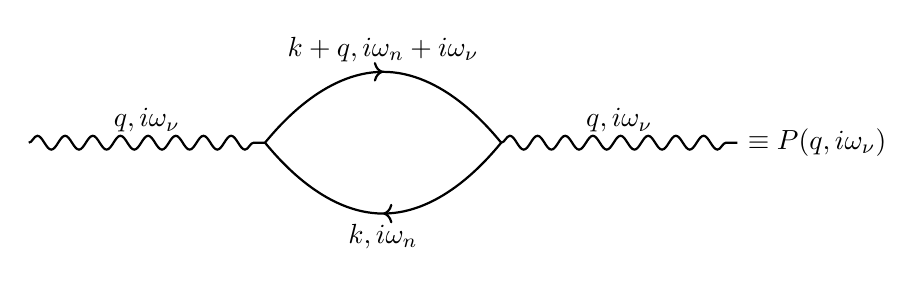
\begin{tikzpicture}[thick, scale = 3]
  	\path [draw = black,snake it]
    (0,0) -- (1,0);
   	\path[draw = black, snake it] (2,0) -- (3,0);
   	\draw[black, ->-=0.5] (1, 0) parabola bend (1.5, 0.3) (2,0);
   	\draw[black, ->-=0.5] (2, 0) parabola bend (1.5, -0.3) (1,0);
   	\node[anchor = south] at (0.5, 0) {$q, i\omega_\nu$};
   	\node[anchor = south] at (1.5, 0.3) {$ k + q, i\omega_n + i\omega_\nu$};
	\node[anchor = north] at (1.5, -0.3) {$ k,i\omega_n$}; 
    \node[anchor = south] at (2.5, 0) {$q, i\omega_\nu$};
    
    \node[anchor = west] at (3,0) {$\equiv P(q, i\omega_\nu)$};
\end{tikzpicture}
	\caption{Feynman diagram}
	\label{fig:feyn_diag}
\end{figure}


\begin{align*}
    P(q, i\omega_\nu) \sim \frac{1}{\beta}\sum_{k, \omega_n}G_0(k, i\omega_n)G_0(k+q, i\omega_n + i\omega_\nu) \\ = \sum_{k} \frac{1}{\beta} \sum_{\omega_n} \frac{1}{i\omega_n - \varepsilon_k}\frac{1}{i\omega_n + i\omega_\nu - \varepsilon_{k+q}}
\end{align*}

The frequency summation is easy: 

\begin{align*}
    \frac{1}{\beta} &\sum_{\omega_n} \frac{1}{i\omega_n - \varepsilon_k}\frac{1}{i\omega_n + i\omega_\nu - \varepsilon_{k+q}} \\ = \frac{1}{i\omega_\nu + \varepsilon_k - \varepsilon_{k+q}} \frac{1}{\beta}&\sum_{\omega_n}\left(\frac{1}{i\omega_n - \varepsilon_k} - \frac{1}{i\omega_n + i\omega_\nu - \varepsilon_{k+q}} \right)
\end{align*}


Now look at the general expression
\begin{align*}
    \frac{1}{\beta}\sum_{\omega_n} \frac{1}{i\omega_n - x} = -\frac{1}{2\pi i}\oint \dd z \frac{f(z)}{z - x} = \frac{-2\pi i}{-2\pi i} f(x) = f(x),
\end{align*}

making the path deformation like in Figure \ref{fig:poles}. This expression implies

\begin{figure}
	\centering
	\begin{tikzpicture}[scale = 2]


%%% Upper left
\draw [-, thick] (0, 1) to (2, 1) ;
\draw [-, thick] (1, 0.1) to (1,1.9) ;
\foreach \y in {0.1,0.3, 0.5, 0.7, 0.9, 1.1, 1.3, 1.5, 1.7, 1.9}
	\node at (1, \y) {$\cross$};
\draw[red,thick,dashed,   ->] (1.2, 0.6) to [in = 0,out = 90] (1, 2) to [in = 90, out = 180] (0.8, 1.4);
\draw[red,thick, dashed, ->] (0.8, 1.4) to [in = 180,out = 270] (1, 0) to [in = 270, out = 0] (1.2, 0.6);
\node at (1.4, 1) (e){$\cross$};
\draw[] (e) node[anchor = north west] {$x$};
\node[anchor = west] at (1.2, 0.4) {$\sim C$};
\node[anchor = west] at (2,1) {$=$}; 

\pgfmathsetmacro\offsetx{2.2}

%%% Upper right
\draw [-, thick] (0+\offsetx, 1) to (2 + \offsetx, 1) ;
\draw [-, thick] (1+\offsetx, 0) to (1+\offsetx,2) ;
\node at (1.4 + \offsetx, 1) (e){$\cross$};
\draw[red, thick, dashed] (0+\offsetx,1.05) to (1.3+\offsetx, 1.05);
\draw[red, thick, dashed, -] (1.3 + \offsetx, 1.05) to [in=90, out = 90] (1.5+\offsetx, 1.05);
\draw[red, thick, dashed, ->] (1.5 + \offsetx, 1.05) to (2+\offsetx,1.05);
\draw[red, thick,dashed] (2 + \offsetx, 0.95) to (1.5+\offsetx, 0.95);
\draw[red, thick, dashed] (1.5 + \offsetx, 0.95) to [in = 270, out = 270] (1.3+\offsetx, 0.95);
\draw[red, thick, dashed,->] (1.3 + \offsetx,0.95) to (0+\offsetx,0.95);

\pgfmathsetmacro\offsety{-1.7}
\pgfmathsetmacro\offsetx{1.1}

%%% Lower picture

\node[anchor = west] at (\offsetx - 0.2,1 + \offsety) {$=$};
\draw [-, thick] (0+\offsetx, 1+\offsety) to (2 + \offsetx, 1+\offsety) ;
\draw [-, thick] (1+\offsetx, 0+\offsety) to (1+\offsetx,2+\offsety) ;
\node at (1.4 + \offsetx, 1+\offsety) (e){$\cross$};
\draw[decoration={markings, mark=at position 0.125 with {\arrow{<}}},
postaction={decorate}, red, dashed, thick] (1.4+\offsetx, 1+\offsety) circle (0.2cm);


\end{tikzpicture}
	\caption{Path deformation}
	\label{fig:poles}
\end{figure}


\begin{equation*}
    P(q,i\omega_\nu)  \sim \frac{\left[ f(\varepsilon_k) - f(\varepsilon_{k+q})\right]}{i\omega_\nu + \varepsilon_k - \varepsilon_{k+q}}. 
\end{equation*}

The f-factors contain all T-effects. Now we can analytically continue: 

\begin{equation*}
    i\omega_\nu \to \omega \pm i\delta \quad \quad \delta = 0^{+}
\end{equation*}

where $+$ and $-$ correspond to retarded and advanced greens functions respectively. From this, we get a dynamical responsefunction for $\omega > 0$ at $T > 0$. 

\section[Interaction \& HS-decoupling]{Interacting fermion-systems and the Hubbard-Stratonovich de-coupling}

\begin{equation*}
    Z = \int \D \left[ \varphi^*\right] \D \left[\varphi\right] \e^{S_0 + S_I}
\end{equation*}

where $S_I$ contain the interaction terms. These terms are typically of the form $\sim \varphi^*\varphi \varphi \varphi^*$, which makes it impossible to calculate the partition function exactly. If $S_I$ is sufficiently small, one uses perturbation theory, which is assumed to be good if $S_I$ doesn't cause qualitative changes in $Z$ relative to $Z_0$ (phase-changes). \\ 

If $S_I$ on the other hand is sufficiently big, which means that it's strong enough to cause phase transitions, we wouldn't be able to detect such changes using perturbation theory at any order. Our strategy will therefore be to approximate $Z$ non-perturbatively around some known free theory. The trick that makes such a calculation possible is the Hubbard-Stratonovich de-coupling of the interacting part of $S$, making $S \to S_{eff}$ into some effective action of the theory. \\

\begin{equation*}
    \e^{S_I} = \e^{-\sum_\lambda \int_{0}^{\beta} \dd \tau H_I(\{ \varphi^*_\lambda, \varphi_\lambda\})}
\end{equation*}

In order to decouple something like this expression, we use the identity

\begin{align*}
    \e^{-\Tr \ln A}\e^{J^*A^{-1}J} = \int \D a^{\dagger} \D a \e^{-a^{\dagger}Aa + J^*a + J\ad}
\end{align*}

where $a,\ad$ are bosonic fields and the sources $J, J^*$ are c-numbers. Now we make the following substitutions 

\begin{equation*}
    J = \varphi \varphi \quad \quad  A^{-1} = V
\end{equation*}

and we get

\begin{equation*}
    e^{S_I}  = \e^{-\Tr \ln A} \int \D a^{\dagger} \D a \e^{-a^{\dagger}V^{-1}a + \varphi^* \varphi^*a + \varphi \varphi\ad}
\end{equation*}

where the first exponent is just a number we can set $=1$, since this only define the zero-point in the free energy. \\ 

Inserting this substitution for $\e^{S_I}$ into the partition function, we end up with 

\begin{equation*}
    Z = \int \D \left[ \varphi^*\right] \D \left[\varphi\right]\D a^{\dagger} \D a \e^{-\varphi^*(\partial_\tau + \varepsilon)\varphi + \varphi^*a\varphi^* + \varphi \ad \varphi - \ad V^{-1}a}. 
\end{equation*}

The point here is that now the fermion part ($\varphi$'s) of the theory is Gaussian, which means that we can integrate out the fermion part of the theory exactly! The interacting fermion theory is formally equivalent to a free fermion theory, coupled to some background bosonic fields. \\ 

\begin{equation}
    Z = \int \D a^{\dagger} \D a \e^{-\ad V^{-1} a} \e^{\frac{1}{2}\Tr \ln G^{-1}}
\end{equation}

where we have inserted the results from 

\begin{align*}
    -\varphi^*(\partial_\tau + \varepsilon)\varphi + \varphi^*a\varphi^* + \varphi \ad \varphi = \\  -\frac{1}{2}\begin{matrix}\begin{pmatrix}\varphi^* & \varphi\end{pmatrix}\mbox{}\end{matrix}
  \begin{pmatrix} \partial_\tau + \varepsilon & -2a \\ -2\ad & \partial_\tau - \varepsilon \end{pmatrix} 
  \begin{pmatrix} \varphi \\ \varphi^* \end{pmatrix} = -\frac{1}{2}\varphi^* G^{-1}\varphi
\end{align*}

where we have introduced fermion spinor notation $\varphi = \begin{pmatrix} \varphi \\ \varphi^* \end{pmatrix}$ and performed a partial integration in $S_I$, resulting in a sign change in the lower right cell of the matrix. 

\begin{align*}
    Z &= \int \D a^{\dagger} \D a \e^{S_{\text{eff}}} \\ 
    S_{\text{eff}}(\ad, a) &= -\sum_\lambda \int_{0}^{\beta} \dd \tau \ad_\lambda(\tau) V^{-1} a_\lambda(\tau) + \frac{1}{2}\Tr \ln G^{-1} 
\end{align*}

Now we have converted our interacting fermion theory into an effective, interacting boson-theory, with effective action $S_eff(\ad, a)$. A priori, this seems like a much more complicated theory compared to the fermion theory we started out with. So what have we accomplished? \\ 

The main point here is that the saddle-point approximation over c-numbers makes sense. A corresponding approximation with Grassmann-numbers doesn't exist. The reason for this is very simple. Say that you want to approximate the integral 

\begin{equation*}
    I = \int \dd x \e^{f(x)}.
\end{equation*}

Now if $f(x)$ has some stable minimum at $x = x_0$, the integral is dominated by the parts close to that minimal value

\begin{align*}
    f(x) = f(x_0) + \frac{1}{2}(x-x_0)f^{''}(x_0) + \cdots \\ 
    I = \approx \e^{-f(x_0)}\int \dd x \e^{-\frac{1}{2}(x - x_0)^{2} f^{''}(x_0)} = \sqrt{\frac{2\pi}{f^{''}(x_0)}}\e^{-f(x_0)}
\end{align*}

Now, if $x$ is a Grassmann-variable, then the taylor expansion is linear $f(x) = c_1 + c_2 x$, and this integral approximation wouldn't have made any sense. We have avoided the problem of calculating the Grassmannian fermion integral approximately, because our Hubbard-Stratonovich de-coupling (HS) mapping made it possible to calculate it exactly! The boson part $\ad, a$ can we, however, try to calculate using our saddle-point approximation. Another way of interpreting this: boson-theories have classical counterparts, whereas fermions doesn't. 

Some remarks: \\

i) The partition function \\

\begin{equation*}
    Z = \int \D \left[ \varphi^*\right] \D \left[\varphi\right]\D a^{\dagger} \D a \e^{J^* a + J \ad - \ad V^{-1}a + S_0(\{\varphi^*,\varphi \})}
\end{equation*}

can be interpreted as the partition function for a non-interacting fermion system which is coupled to a dynamical boson-field, where $S_{eff}(\ad, a)$ is the free energy to this system for a particular configuration of the external fields $\ad,a$. The total free energy is the sum of the free energies of each of the configurations. \\ 

ii) It's important to notice that there is an ambiguity in choosing how to HS decouple the non-interacting part in the fermion sector. We could have just as well chosen to substitute 

\begin{equation*}
    J = \varphi^* \varphi \quad \quad J^* = \varphi^* \varphi
\end{equation*}

instead of our previous choice 

\begin{equation*}
    J = \varphi \varphi \quad \quad J = \varphi^* \varphi^*. 
\end{equation*}

The important thing to note here is that as long as we compute the boson functional integral exactly, it doesn't matter what choice we make. On the other hand, if we compute the boson functional integral approximately, then the choice does matter. Then the choice of decouple scheme is determined by what kind of physics we expect in the end. 

Now we HS decouple $S_I$ in the following manner: 

\begin{align*}
    J = \varphi_\downarrow(x,\tau) \varphi_\uparrow(x, \tau) \\
    J^* = \pu^*(x,\tau) \pd^*(x,\tau) 
\end{align*}

where now $J, J^*$ is pair-fields and $a, \ad$ is their corresponding conjugated fields. Now recall that the trace-exponential, which corresponed to the zero-point energy, was put to zero. Then we get 

\begin{align}
    \e^{S_I} = \e^{VJ^*J} =  \int \D a^{\dagger} \D a \e^{-a^{\dagger} \frac{1}{V}a + J^*a + J\ad} \\ 
    \implies \e^{S_{I}} =  \int \D a^{\dagger} \D a \e^{-\sum_x \left[\frac{1}{V} \abs{a(x)}^{2} - \pu^*(x,\tau) \pd^*(x,\tau)a(x) - \varphi_\downarrow(x,\tau) \varphi_\uparrow(x, \tau)\ad \right]} 
\end{align}

And we get the partition function 

\begin{align*}
    Z = \int \D \left[ \varphi^*\right] \D \left[\varphi\right]\D a^{\dagger} \D a \e^{-\sum_x \frac{1}{V}\ad a + A_z} \\ 
    A_z = S_0 + \sum_x \left[ \ad \varphi_\downarrow(x,\tau) \varphi_\uparrow(x, \tau) + a \pu^*(x,\tau) \pd^*(x,\tau) \right]
\end{align*}

Now we define the Nambu-formalism, which means writing the conjugate fields $\pu, \pd$ as a 2-component spinor in the following way 

\begin{align*}
    \Psi(x) = \begin{pmatrix}\pu(x) \\ \pd^*(x) \end{pmatrix} \quad \quad \Psi^{\dagger} = \begin{pmatrix}\pu^*(x) & \pd(x)\end{pmatrix}
\end{align*}

Now we see that 

\begin{align*}
    \sum_x \left[ \ad \varphi_\downarrow(x,\tau) \varphi_\uparrow(x, \tau) + a \pu^*(x,\tau) \pd^*(x,\tau) \right] \\ 
    = \sum_x \Psi^{\dagger} (x) \begin{pmatrix} 0 & a(x) \\ \ad(x) & 0 \end{pmatrix} \Psi(x) \\ 
    S_0 = -\sum_{x,y} \left[ \pu^*(x)(\partial_\tau + \varepsilon - \mu)\pu(y) + \pd^*(x)(\partial_\tau +\varepsilon - \mu)\pd(x)\right] \\ 
    = -\sum_{x,y} \begin{pmatrix}\pu^* & \pd\end{pmatrix} \begin{pmatrix}(\partial_\tau + \varepsilon - \mu)  & 0 \\ 0 & (\partial_\tau -(\varepsilon - \mu)) \end{pmatrix} \begin{pmatrix}\pu \\ \pd^* \end{pmatrix} \\ 
    = -\sum_{x,y} \Psi^{\dagger}(x) \left[ -G_0 ^{-1}(x,y) \right] \Psi(y) 
\end{align*}

Combining all expressions, we get 

\begin{align*}
    A_z = -\sum_{x,y} \Psi^{\dagger}(x)\left[ -G ^{-1}(x,y) \right]\Psi(x) \\
    -G ^{-1}(x,y) = -G_0 ^{-1}(x,y) - B(x)\delta_{x,y} \\ 
    B(x) = \begin{pmatrix} 0 & a(x) \\ \ad(x) & 0 \end{pmatrix} 
\end{align*}

Note that here the fermion propagator $G \sim - \expval{\Psi \Psi^{\dagger}}$ is a 2x2-matrix acting in Nambu spinor-space. The partition function now becomes 

\begin{align*}
    Z = \int \D \left[ \Psi^{\dagger}\right] \D \left[\Psi\right]\D a^{\dagger} \D a \e^{-\sum_x \frac{1}{V}\ad a -\sum_{x,y} \Psi^{\dagger}(x)\left[ -G ^{-1}(x,y) \right]\Psi(x)} \\ 
    = \int \D a^{\dagger} \D a \e^{-\sum_x \frac{1}{V}\ad a + \Tr \ln \left(-G ^{-1}\right)} \\ 
    = \int \D a^{\dagger} \D a \e^{S_{eff}(\ad, a)} \\ 
    S_{eff} = -\sum_x \frac{1}{V}\ad a + \Tr \ln \left(-G_0 ^{-1}(x,y) -B(x)\delta_{x,y}\right)
\end{align*}

This partition function has now been transformed into a pure bosonic problem. Saddle-point approximation to this integral gives mean field theory. Here the trace $\Tr = \sum_{x} \tr$, where $\tr$ is a 2x2-matrix trace. \\ 

Mean field theory (MFT): $a(x) \to a$ constant. \\

\begin{equation*}
    \Tr \ln \left(-G ^{-1}(x,y)\right) = \sum_x \tr \ln \left(-G ^{-1}(x,y)\right) = \sum_k \tr \ln \left(-G ^{-1}(k)\right)
\end{equation*}

\subsection{BCS-theory}

\begin{align*}
    Z = \int \D \varphi^* \D \varphi \e^S \\ 
    S = S_0 + S_I = -\sum_\lambda \varphi_\lambda^* \pdv{\varphi_\lambda}{\tau} + H\left(\varphi_\lambda^*, \varphi_\lambda \right) \\ 
    S_0 = \sum_{x,y,\sigma} \varphi_\sigma ^* (x) \left( \partial_\tau + \varepsilon - \mu \right) \varphi_\sigma (y) \\ 
    H_I = -V \sum_x \nuu(x) \nd(x) \quad \quad V > 0 \\ 
    S_I = V\sum_x \nuu(x) \nd(x) \quad \quad V > 0
\end{align*}

Attractive interaction for electrons with opposite spin (Retarded). \\ 
\begin{align*}
    S_I = V \sum_x \pu^*(x) \pd^* (x) \pd(x) \pu(x) \\ 
    \e^{S_I} = \int \D\ad \D a \e^{-\sum_x \left( \frac{\ad a}{V} - a \pu^* \pd^* - \ad \pd \pu \right)} \\ 
    \varphi = \begin{pmatrix} \pu \\ \pd^* \end{pmatrix} \quad \quad \varphi^\dagger = \begin{pmatrix} \pu^* & \pd \end{pmatrix} \\ 
    \e^{S_I} = \int \D\ad \D a \e^{-\sum_x \left( \frac{\ad a}{V} + \sum_x \varphi^\dagger (x) B(x) \varphi(x) \right)}
\end{align*}

Where $B(x)$ is the same matrix as in the last section. 

\begin{align*}
    S_0 = -\sum_{k, \sigma} \int_{0}^{\beta} \dd \tau \left[ \varphi_{k\sigma} ^* (\tau) \left( \partial_\tau + \varepsilon_k - \mu \right) \varphi_{k \sigma} (\tau) \right] 
\end{align*}

where we have done the following partial Fourier transformation 

\begin{equation*}
    \varphi_\sigma^*(x,\tau) \to \varphi^*_{k \sigma}(\tau).
\end{equation*}

Now we do the spin summation: 

\begin{align*}
    -\sum_k \int_{0}^{\beta} \dd \tau \left[ {\pu}_{k}^* (\tau) \left( \partial_\tau + \varepsilon_k - \mu \right) {\pu}_{k} (\tau) + {\pd}_{k}^* (\tau) \left( \partial_\tau + \varepsilon_k - \mu \right) {\pd}_{k} (\tau)\right].
\end{align*}

Look at the last term: 

\begin{align*}
    \sum_k \int_{0}^{\beta} \dd \tau \left[{\pd}_{k} ^* (\tau) \left( \partial_\tau + \varepsilon_k - \mu \right) {\pd}_{k} (\tau)\right] \\ 
    = \sum_k \int_{0}^{\beta} \dd \tau \left[{\pd}^*(k) \pdv{{\pd}_k}{\tau} + {\pd}_{k} ^* (\tau) \left(\varepsilon_k - \mu \right) {\pd}_{k} (\tau)\right] \\ 
    = \sum_k \eval{{\pd}_k^* {\pd}_k}_0 ^\beta + \int_{0}^{\beta} \dd \tau \left[{\pd}(k) \pdv{{\pd}^*_k}{\tau} - {\pd}_{k} (\tau) \left(\varepsilon_k - \mu \right) {\pd}_{k}^* (\tau)\right] \\ 
    = \sum_k \int_{0}^{\beta} \dd \tau \left[{\pd}(k) \pdv{{\pd}^*_k}{\tau} - {\pd}_{k} (\tau) \left(\varepsilon_k - \mu \right) {\pd}_{k}^* (\tau)\right]
\end{align*}

where we have performed a partial integration, which effectively reduced to changing the derivative and sign since the fields are periodic on $[0, \beta]$. This change of sign is cancelled by the anti-commutation of the fermionic fields. The sign of the last term also changed due to interchange of the fields. Fourier transforming back into real space and combining this with the other part of $S_0$, we get 

\begin{align*}
    S_0 = -\sum_{x,y} \left[ \pu^*(x)(\partial_\tau + \varepsilon)\pu(y) + \pd(x) (\partial_\tau - \varepsilon)\pd^*(y) \right] \\ 
    = -\sum_{x,y} \varphi^\dagger (x)\begin{pmatrix}(\partial_\tau + \varepsilon)  & 0 \\ 0 & (\partial_\tau -\varepsilon) \end{pmatrix} \varphi(y)
\end{align*}

\begin{align*}
    Z = \int \D \varphi^\dagger \D \varphi \D \ad \D a \e^{-\sum_x \frac{\ad (x) a}{V}} \e^{-\sum_{x,y} \varphi(x)^\dagger G^{-1}(x,y)\varphi(y)} \\ 
    G^{-1}(x,y) = G_0 ^{-1} (x,y) - B(x) \delta_{x,y} \\
    G_0^{-1}(x,y) = \begin{pmatrix}(\partial_\tau + \varepsilon)  & 0 \\ 0 & (\partial_\tau -\varepsilon) \end{pmatrix}
\end{align*}

Now perform the $\varphi$ integrations: 

\begin{align*}
    \int \D \ad \D a \e^{S_{eff}[a, \ad]} \\ 
    S_{eff}[a, \ad] = -\sum_x \frac{\ad(x) a(x)}{V} + \Tr \ln [G^{-1} ],
\end{align*}

which is an exact result! Now we move on to mean field approximation: $a(x) \to a$. 

\begin{align*}
    \Tr \ln [G^{-1}] = \frac{1}{\beta} \sum_k \sum_{\omega_n} \tr \ln G^{-1} (k, i\omega_n), \\ 
    G^{-1}(k, i\omega_n) = \begin{pmatrix}-i\omega_n + \varepsilon_k  & -a \\ -\ad & -i\omega_n -\varepsilon_k \end{pmatrix}
\end{align*}

\begin{align*}
    \tr \ln G^{-1} = \ln \det{G^{-1}} = \ln((i\omega_n)^2 - \e_k^{2} -\abs{a}^{2}) = \ln(i\omega_n - E_k) + \ln(i\omega_n + E_k) \\ 
    \implies S_{eff}^{MF} = -\frac{N\beta \abs{a}^2}{V} + \sum_k \ln \left[ (1+\e^{-\beta E_k})(1 + \e^{\beta E_k})\right] = -\beta F^{MF} \\ 
    \implies f^{MF} = \frac{F^{MF}}{N} = \frac{\abs{a}^2}{V} +\frac{1}{\beta} \frac{1}{N}\sum_k \ln \left[ (1+\e^{-\beta E_k})(1 + \e^{\beta E_k})\right].
\end{align*}

Since $S_{eff}$ is exact, we automatically have a recipe for how we can correct mean-field theory, and also a recipe for how to check it's stability. 

\begin{align*}
    G^{-1}(k) = \begin{pmatrix}-i\omega_n + \varepsilon_k  & -a \\ -\ad & -i\omega_n -\varepsilon_k \end{pmatrix} \\ 
    \implies G(k) = \frac{-1}{(i\omega_n)^2 - E_k^{2}} \begin{pmatrix}i\omega_n + \varepsilon_k  & a \\ \ad & i\omega_n - \varepsilon_k \end{pmatrix} = \expval{\Phi \Phi^\dagger} 
\end{align*}

where $E_k = \sqrt{\varepsilon_k ^2 + \abs{a}^2}$ and we compare with 

\begin{align*}
    G(k) \to -G_F(k) \implies G_F = - \expval{\Phi \varPhi^\dagger}
\end{align*}

\begin{align*}
    \tr \ln \left[-G_f ^{-1} (k) \right] = \ln \det(-G_F {-1} (k)) = \ln(i\omega_n - E_k) + \ln(i\omega_n + E_k)\\ 
    \sum_k \tr \ln \left[-G_f ^{-1} (k) \right] = \sum_k \frac{1}{\beta} \sum_{\omega_n} \left[ \ln(i\omega_n - E_k) + \ln(i\omega_n + E_k) \right]
\end{align*}

Earlier we showed that 

\begin{align*}
    \frac{1}{\beta}\sum_{\omega_n} \ln(i\omega_n - x) = \ln(1 + \e^{-\beta x}) \\ 
    \implies \sum_x \tr \ln(-G_F ^{-1}(k)) = \sum_k \left[\ln(1 + \e^{-\beta E_k}) + \ln(1 + \e^{\beta E_k})\right] 
\end{align*}

\begin{align*}
    \sum_x \frac{\abs{a(x)}^2}{V} = \beta N \frac{\abs{a}^2}{V} \\ 
    Z_{MF} = \e^{-\beta F_{MF}} = \e^{-\beta N \frac{\abs{a}^2}{V}} \e^{\sum_k \left[\ln(1 + \e^{-\beta E_k}) + \ln(1 + \e^{\beta E_k})\right]} \\ 
    \frac{F_{MF}}{N} = \frac{\abs{a}^2}{V} - \frac{1}{\beta} \frac{1}{N}\sum_k \left[\ln(1 + \e^{-\beta E_k}) + \ln(1 + \e^{\beta E_k})\right]
\end{align*}

where $a$ is determined by minimizing the free energy. 

\begin{align*}
    \pdv{}{a}f_{MF} = 0 \implies \frac{2a}{V} - \frac{1}{N}\sum_k \frac{2a}{2E_k}\left(\frac{e^{\beta E_k}}{1 + \e^{\beta e_k}} - \frac{e^{-\beta E_k}}{1 + \e^{-\beta e_k}} \right) = 0 \\
    2a \left[\frac{1}{V} - \frac{1}{N}\sum_k \frac{1}{2E_k}\left(\frac{e^{\beta E_k}}{1 + \e^{\beta e_k}} - \frac{e^{-\beta E_k}}{1 + \e^{-\beta e_k}} \right) \right] = 0 \\ 
    \frac{1}{V} = \frac{1}{N} \sum_k \frac{\tanh(\frac{\beta E_k}{2})}{2E_k}
\end{align*}

This is the gap-equation for BCS-theory! The advantage of solving it this way, is that now we know how to include fluctuations. \\ 

To check that this is in fact a minimum, we check the curvature of the free energy at this value $a_0$

\begin{align*}
    \pdv{^2 f_{MF}}{a^2} = \pdv{}{a} 2a \left[\frac{1}{V} - \frac{1}{N}\sum_k \frac{1}{2E_k}\left(\frac{e^{\beta E_k}}{1 + \e^{\beta e_k}} - \frac{e^{-\beta E_k}}{1 + \e^{-\beta e_k}} \right) \right] \\ = 2\left[\frac{1}{V} - \frac{1}{N}\sum_k \frac{1}{2E_k}\left(\frac{e^{\beta E_k}}{1 + \e^{\beta e_k}} - \frac{e^{-\beta E_k}}{1 + \e^{-\beta e_k}} \right) \right] \\ - 2a \frac{1}{N} \sum_k \pdv{}{E_k}\left(\frac{1}{2E_k}\tanh(\frac{\beta E_k}{2})\right) \pdv{E}{a}.
\end{align*}

By the gap-equation, we see that the first term is $0$ at $a_0$. Taking the derivative of the last term, we end up with 

\begin{align*}
    \frac{a^2}{N}\sum_k \frac{1}{E_k ^3} \frac{1}{\cosh^2(\frac{\beta E_k}{2})} \left(\sinh(\beta E_k) - \beta E_k \right) > 0 \quad \forall \beta E_k.
\end{align*}
Thus the free energy has a global minimum at $a = a_0$, which means that the solution is unique in the case of contact-interactions. 

\subsection{Stationary point condition} 

\begin{align*}
    \pdv{f^{MF}}{b^2} = 0 \implies -\lambda + \frac{1}{N}\sum_k \frac{\e^{-\beta \ep_k}}{1 + \e^{-\beta \ep_k}} \pdv{\ep_k}{b^2} = 0 \\
    \pdv{f^{MF}}{\lambda} = 0 \implies -1 + b^2  + \frac{1}{N}\sum_k \frac{\e^{-\beta \ep_k}}{1 + \e^{-\beta \ep_k}} \pdv{\ep_k}{\lambda} = 0. 
\end{align*}

We also have the constraint 

\begin{equation*}
    n = - \pdv{f^{MF}}{\mu} = \frac{1}{N}\sum_k f(\ep_k),
\end{equation*}

which is the number of fermion constraint 

\begin{equation*}
    \implies n = 1 -b^2 \implies n + b^2 = 1.
\end{equation*}

Look at the spectrum compared to the free theory

\begin{align*}
    \ep_k^{MF} = -2tb^2 \gamma_k - (\lambda + \mu) \\
    \ep_k ^{free} = -2t\gamma_k \mu 
\end{align*}

We see that $\lambda$ renormalizes the chemical potential $\mu$ in order for $\expval{Q_i} = 1$ to be fulfilled. We also see that $b^2$ renormalizes the gap-width, correlation effect, $Q_i = n +b^2 = 1$. \\

Now look at the case $n = 1$, i.e. half-filled band. Thus $b^2 = 0$, and therefore 

\begin{equation*}
    \ep_k = -(\lambda + \mu) = \ep_k
\end{equation*}

The energy spectrum is independent of $k$! This means that we have localized fermions. No movement, no momentum exitations $k$. Thus, in mean-field theory, we have an insulator at $U = \infty$ half-filled band. Mean field theory also predict that $b^2 > 0 ; n < 1$, i.e. that when the system is doped away from half-filled band. In this case, still using mean field theory, we get a metal. Thus by doping the system away from half-filled bands, we go from an insulator to a metal. Near half-filled band, the gap is very small, i.e. that the quasiparticels are effectively very massive 

\begin{equation*}
    m^* \sim \frac{1}{b^2} \quad \quad b \to 0 \implies m^* \to \infty 
\end{equation*}

Preciely at half-filled band, the model is a very simple insulator. It reduces to the Heisenberg model 

\begin{align*}
    H = -J \sum_{\expval{i,j}} \Vec{S}_i \cdot \Vec{S}_j \quad \quad J \sim \frac{t^2}{U} \to 0 \quad  ; \quad U \to \infty 
\end{align*}

\begin{align*}
    S_{eff} = -\sum_i \int_{0}{\beta} \dd \tau \bd_i (\partial_\tau + i\lambda_i)b_i + i\sum_i \int_{0}{\beta} \lambda_i(\tau) + \Tr \ln(G^{-1}) \\ 
    S_{eff}^{MF} = - N\beta (b^2 - 1)\lambda \sum_k \ln (1 + \e^{-\beta \ep_k})  \\ 
    \ep_k = -2tb^2\gamma_k - (\lambda + \mu) 
\end{align*}

Again, the exact expression makes it possible to do corrections to mean field theory. We may come back to this later. \\

In this saddle point approximation, we have $\expval{b} \neq 0$. Look at the Hamiltonian 

\begin{equation*}
    H = - \sum_{i,j,\sigma} t_{ij} d^{\dagger}_{i \sigma} b_i \bd_j d_{j \sigma}.
\end{equation*}

We see that the following symmetry isn't broken 

\begin{align*}
    b_i \to b_i \e^{i\theta} \\ 
    d_i \to d_i \e^{i\theta} 
\end{align*}

since the creation operators $\bd, d^{\dagger}$ cancel the phase-factor, which again keeps the Hamiltonian invariant. Thus the Hamiltonian is still invariant under global $U(1)$ transformations, even tho $\expval{b} \neq 0$. On the other hand, by introducing the bosons $\bd, b$, the symmetry has improved to a local $U(1)$ symmetry

\begin{align*}
    b_i \to b_i \e^{i\varphi_i} \\ 
    d_i \to d_i \e^{i\varphi_i}. 
\end{align*}

It is this symmetry which is broken at the saddle-point, because then the boson-fields have acquired a finite expectation value $\expval{b} \neq 0$. If the local $U(1)$ symmetry had not been broken, the expectation value would have vanished due to the fluctuations associated with the symmetry. Again $\expval{b}$ can be interpreted as a order parameters, but for what? To answer this, we look at the spectrum, similar to what we did in the superconductor case

\begin{equation*}
    \ep_k = -2tb^2 \gamma_k - (\lambda + \mu). 
\end{equation*}

When $b \neq 0$, we have dispersion, but when $b = 0$, $\ep_k$ is independent of $k$. Localized quasiparticles in the system implies that the system is an insulator. $b$ is therefore an order parameter for metal. \\ 

Equivalently: The local $U(1)$ invariance means that we have conservation of particle number at each site $i$. This means that the particles in the system are confined/localized. If we again look at the original Hamiltonian 

\begin{equation*}
    H = -t \sum_{\expval{i,j}}c_{i\sigma}^\dagger c_{j\sigma} - \mu \sum_{i, \sigma}c_{i\sigma}^\dagger c_{i\sigma},
\end{equation*}

we see that as long as we have hopping $t$, there are no local $U(1)$ invariance. As long as the fermions are moving, this symmetry is broken. If however the hopping isn't operative, which implies localized fermions, the system has local $U(1)$. Again we reach the conclusion that if the local $U(1)$ symmetry is broken, the number of localized fermions is not conserved, which means that they are mobile, i.e. metallic system. $\expval{b} \neq 0 \implies$ broken local $U(1)$ invariance $\implies \expval{b}$ order parameter for metal. \\

Generally, the conductivity of a translationally invariant system is of the form 

\begin{equation*}
    \sigma (\omega) = D\delta (\omega) + \sigma_{reg}(\omega). 
\end{equation*}

Thus a translationally invariant system has infinite d.c. conductivity. $D$ is often called the rigid conductivity, or the Drude-weight. In our model, $D \sim b^2$. Many years ago, Walter Kohn suggested using $D$ as the order parameter for a metallic system (non-zero drude weight). Our example above show that this wasn't a bad suggestion. \\

The problem of describing an insulator-metal phase transitions is a notoriously hard problem. The fact that we find this using this very simple approximation really show the potential of the functional integral formalism, especially in strongly correlated systems. Free theory with half-filled band is a good metal, not an insulator. It would have been hopeless to find this transitions using perturbation theory, similarly for the metal-superconductor phase transition. Note that this mean field theory predict that, even for $U \to \infty$, the Hubbard model is always a Fermi liquid away from half-filled band. In one dimention, we know this is wrong, since every interacting one-dimensional system is a Luttinger liquid. This is a quantum liquid without low-energy one-particle exitations. In one dimention, interactions are always effective, because of the restriction of the kinematics. Particles cannot pass each other without colliding in one-dimention, in contrast to higher dimensional systems, where Fermi liquids are possible. \\

In three dimension, our mean field theory should be qualitatively correct. In two-dimension, there are indications that strongly correlated systems can have non-fermi liquid behaviour, so mean field theory is not the end of the story. We might later on look at what happens when we turn on fluctuations in this model. Then the quasiparticles starts interacting with the fermions we found using mean field theory. The result is: superconductivity! \\ 


\section[Broken symmetries]{Broken continuous symmetries and Goldstone-modes}

Both of the previous examples, the BCS- and Hubbard-model, have shown that a system where the Hamiltonian is invariant under a continuous symmetry group ($U(1)$ in both cases), the ground state, which the system chooses, doesn't need to respect the symmetry. This are examples of broken symmetries, and because the system ``breakes it on its own'', we say that the systems have spontaneously broken (continuous) symmetries. In the following, we will examine an important consequence of these broken symmetries. Note that this does not apply to discrete symmetries, like e.g. Ising-model.  

BCS-model: 

\begin{equation*}
    f^{\text{MF}}(\ad, a) = f(\abs{a}^2) \quad \expval{\ad} \neq 0 \neq \expval{a}.
\end{equation*}

$U = \infty$ Hubbard model: 

\begin{equation*}
    f^{\text{MF}}(\bd, d) = f(\abs{b}^2) 
\end{equation*}

\begin{equation*}
    \abs{\Delta} = \abs{a}, \abs{b}. 
\end{equation*}

In \cref{fig:free_broken1} we see that there is two global minima of $f^{\text{MF}}$ for non-zero $\Delta$'s. These are both stable. 
\begin{figure}
	\centering
	\begin{subfigure}{0.4\textwidth}    
		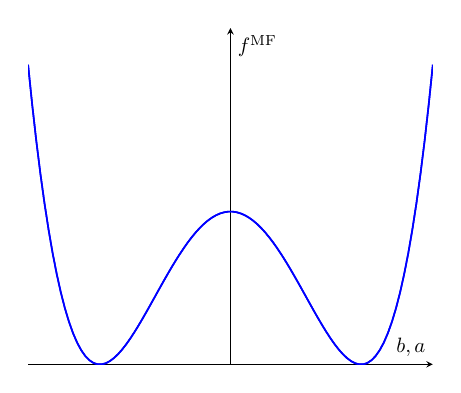
\begin{tikzpicture}[scale=0.75]
	\begin{axis}[
	ticks = none,
	xlabel = {$b,a$},
	ylabel = $f^{\text{MF}}$,
	x label style={at={(axis description cs:1,0.1)}, anchor = west},
	y label style={at={(axis description cs:0.15,1)},rotate=-90,anchor=south},
	ymax = 2,	
	axis lines = middle]
	
	
	
	\addplot[thick,
	domain=-2:2, 
	samples=100, 
	color=blue]{- x^2 + 0.3*x^4 + 1};
	
	\end{axis}
      %\draw[->] (-4,0) -- (4,0) node[right] {$b, a$};
      %\draw[->] (0,-4) -- (0,4) node[above] {$f^{MF}$};
      %\draw[blue] plot[samples=200,domain=-2:2] function {};
\end{tikzpicture}
		\caption{$|\Delta| \ne 0$}
		\label{fig:free_broken1}
	\end{subfigure}
	\hfill
	\begin{subfigure}{0.4\textwidth}
		\begin{tikzpicture}[scale = 0.75]
	\begin{axis}[
	ticks = none,
	xlabel = {$b,a$},
	ylabel = $f^{\text{MF}}$,
	x label style={at={(axis description cs:2,0.1)}, anchor = west},
	y label style={at={(axis description cs:0.15,2)},rotate=-90,anchor=south},
	ymax = 4,	
	axis lines = middle]
	
	
	
	\addplot[thick,
	domain=-2:2, 
	samples=100, 
	color=blue]{0.7*x^2 + 0.5};
	
	\end{axis}



      %\draw[->] (-4,0) -- (4,0) node[right] {$b, a$};
      %\draw[->] (0,-4) -- (0,4) node[above] {$f^{MF}$};
      %\draw[blue] plot[samples=200,domain=-2:2] function {};
\end{tikzpicture}
		\caption{$|\Delta| = 0$}
		\label{fig:free_broken_2}	
	\end{subfigure}
	\label{fig:free_broken}
\end{figure}

\begin{equation*}
    \pdv{f^{\text{MF}}(\Delta^2)}{\Delta} = 2\Delta f^{'}(\Delta^2) 
\end{equation*}

\begin{equation*}
     \abs{\Delta} = 0
\end{equation*}

In \cref{fig:free_broken_2} we see that $f^{\text{MF}}$ has one global minima at $\Delta = 0$. This minima is also stable. 

We have seen that generally $\expval{a}$ and $\expval{b}$ are complex order parameters. We can therefore treat $f^{\text{MF}}$ as a function of a complex variable, while it is independent of the phase of the complex number. In the case of $\abs{\Delta} = 0$, the phase is ill-defined at $f^{\text{MF}}_{min}$. In the case of $\abs{\Delta} \neq 0$, the situation is a little bit different. Then we can rotate the corresponding graph around the y-axis ($f^{\text{MF}}$), and we obtain the following kind of graph

% \begin{figure}
%     \centering
% \begin{tikzpicture}[scale =1.5]
%     \begin{axis}[
%         hide axis,
%         samples=50,
%         domain=0:360,
%         y domain=0:1.25
%         ]
%     \addplot3 [surf, shader=flat, draw=blue!70!white, fill=white, z buffer=sort] ({sin(x)*y}, {cos(x)*y}, {(y^2-1)^2});
%     \end{axis}
% \end{tikzpicture}
%     
% \end{figure}


We see that the minima of the free energy is infinetly degenerate, because it is independent of the phase $\varphi$: 

\begin{align*}
    f^{\text{MF}}(\Delta, \Delta^*) = f^{\text{MF}}(\abs{\Delta}, \varphi) = f^{\text{MF}}(\abs{\Delta}) \\
    \Delta = \abs{\Delta}\e^{i\varphi}. 
\end{align*}

This means that phase fluctuations cost no energy, but fluctuations in the radial $\abs{\Delta}$ direction does.
\begin{itemize}
	\item $\abs{\Delta}$-amplitude fluctuations: Longitudinal fluctuations.
	\item $\varphi$-fluctuations: Transverse fluctuations. 
\end{itemize}

We say that the longitudinal fluctuations are "massive" and the traversal fluctuations are "massless". The massless fluctuations correspond to Goldstone-modes, which has a finite interaction range. We have seen that a broken symmetry ($\Delta \neq 0$) means that there exist Goldstone-modes. 

In our case, the order parameter where comples, which means that it has two real components. Here we got one infinite degeneracy in the phase, which corresponded to one Goldstone mode. Generally in our study, if $\Delta$ has n components, we get $n-1$ Golstone-modes.  

The existence of the Goldstone-modes makes it apparently problematic to define a fluctuation-calculation around the stationary point, since the Goldstone-modes corresponds to (at least one) zero eigenvalue of the fluctuation propagators. 
\begin{align*}
    S = S^{\text{MF}} + \Tr \ln D^{-1} \\ 
    Z = \e^{S^{\text{MF}}}\frac{1}{\det D^{-1}} \\ 
    D^{-1} = \prod_i \lambda_i \quad \quad \exists j : \lambda_j = 0 
\end{align*}

In order to investigate small fluctuations around a mean-field theory, it is of course intolerable to have this problem. It turns out that this is an apparent problem which we can avoid, as we will see. 

We will look at Gaussian fluctuations around a spontaneously broken continuous symmetry. The following effective action isn't approximated, but we will for the sake of the argument and simplicity look at a real field with real rotational invariance (e.g. XY-model, where the spins can point in any direction in the plane). I emphasise however that the discussion is general. 

\begin{align*}
    Z = \int \D \p \e^{S[\p]} \\ 
    \fdv{S}{\p} = 0 \quad \quad  \p = \p_0
\end{align*}

where $\p$ is a function of $x = (\Vec{x_0}, \tau)$. $\p_0$ contains a parameter $\theta$ which describe the symmetry-transformation of the symmetry that is spontaneously broken. It can e.g. be the parameter describing the ground state degeneracy ("circular minimum") in the rotated graph of $f^{\text{MF}}$ above. We expand to gaussian order in $S$:

\begin{align*}
    Z = \e^{S^{\text{MF}}}\int \D \p \e^{-\frac{1}{2}\sum_{x,y} (\p(x) - \p_0(x)) A (\p(y) - \p_0(y))} \\
    A = \fdv{^2S}{\p_0(x) \delta \p_0(y)}
\end{align*}

Naively, this will be something like 

\begin{align*}
    Z = \e^{S^{\text{MF}}} \frac{1}{\sqrt{\det A}}
\end{align*}

but because of the Goldstone-modes, there is an apparent divergence in the fluctuations due to the zero eigenvalue. It seems like any attempt at doing mean-field theory when the symmetry is broken is doomed to fail. Nevertheless, we know that e.g. the mean-field theory of BCS-theory is a very good approximation without any divergences. There must be a reason for why this is the case.  

In order to avoid such divergences, the idea is to split the fluctuations into longitudinal- and transverse components. Recall that the longitudinal components are the "massless" components, which are associated to the degeneracy of the ground state, and the transverse are the "massive" components associated to the fluctuations in the radial, or amplidude, direction. The functional derivative 

\begin{equation*}
    A = \fdv{^2S}{\p_0(x) \delta \p_0(y)}
\end{equation*}

must be diagonalized in order to find the fluctuation corrections. The problem is, however, that the presence of zero eigenvalues makes this impossible. The corresponding eigenvectors of these eigenvalues, namely the Goldstone-modes, are the components of the fluctuation vector $\p(x) - \p_0(x,\theta)$ with zero eigenvalue.  

\begin{align*}
    A \cdot x = \lambda x \\ 
    A \cdot x_G = 0 \\ 
    A \cdot x_{\perp} \neq 0 \\ 
    x_{\perp} \cdot x_G = 0
\end{align*}

Define the "inner-probduct" 

\begin{align*}
    \int \dd x (\p(x) - \p_0(x))_{\perp} (\p(x) - \p_0(x))_G
\end{align*}

At the stationary point, we have (independent of the value of $\theta$) 

\begin{align*}
    \fdv{S}{\p_0(x,\theta)} = 0 \implies \pdv{}{\theta} \left(\fdv{S}{\p_0(x,\theta)}  \right) = 0 
    \implies \int \dd y \fdv{^2S}{\p_0(x) \delta \p_0(y)} \pdv{\p_0(y,\theta)}{\theta} \\ 
    = \int \dd y A(x,y)\pdv{\p_0(y,\theta)}{\theta} = A \cdot \pdv{\p_0(y,\theta)}{\theta} = 0 
    \implies \pdv{\p_0(y,\theta)}{\theta} = x_G
\end{align*}

where we have identified the explicit form of the Goldstone-mode. The next step is to split up the fluctuations into the Goldstone-mode and components "vertical" to this. We do this by using the inner-product as a projection, defining 

\begin{equation*}
    f(\theta) = \int \dd x \pdv{\p_0(y,\theta)}{\theta} [-\p(x) + \p_0(x)].
\end{equation*}

the components of $[-\p(x) + \p_0(x)]$ orthogonal to the Goldstone-mode $\pdv{\p_0(y,\theta)}{\theta}$, the verical components, are therefore the once corresponding to $f(\theta) = 0$. We can therefore write: 

\begin{align*}
    \p(x) - \p_0(x,\theta) = \begin{pmatrix} \pdv{\p_0(y,\theta)}{\theta} \\ (\p(x) - \p_0(x,\theta))_{\perp} \end{pmatrix}
\end{align*}

using this notation, we can write 

\begin{align*}
    (\p(x) - \p_0(x)) A(x,y) (\p(y) - \p_0(y)) \\ 
    = \begin{pmatrix} \pdv{\p_0(y,\theta)}{\theta} && (\p(x) - \p_0(x,\theta))_{\perp} \end{pmatrix} \begin{pmatrix} A_G && 0 \\ 0 && A_{\perp} \end{pmatrix} \begin{pmatrix} \pdv{\p_0(y,\theta)}{\theta} \\ (\p(x) - \p_0(x,\theta))_{\perp} \end{pmatrix}
\end{align*}

The problem now amounts to $A_G = 0$. \\ 

\begin{equation*}
    \det A = \det A_G \det A_{\perp} = 0
\end{equation*}

$A_G = 0$ because the energies associated with the quadratic Goldstone-mode fluctuations is zero. The trick now is to define $A_G = \varepsilon$ (one Goldstone-mode), such that the determinant $\det A = \varepsilon \det A_{\perp} \neq 0$. After the gaussian integrations have been done, $\varepsilon$ is set to zero. Do we get something finite? \\ 

We wish to split the functional integral into two contributions, one over Goldstone-modes, $f = 1$, and one over longitudinal modes, $f = 0$. \\ 

\begin{align*}
    \int \dd f \delta (f) = 1 \\ 
    \int \dd \theta \dv{f}{\theta} \delta(f) = 1 \\
\end{align*}

The point here is: the delta function $\delta (f)$ only contributes when $f = 0$. \\ 

\begin{align*}
    Z = \e^{S_{\text{MF}}}\int \D \psi \e^{-\frac{1}{2}\sum_{x,y} \psi(x) A \psi(y)}
\end{align*}

General fluctuations vector \\ 

\begin{align*}
    \psi = \phi(x) - \phi_{0}(x,\theta) = 1
    Z = Z = \e^{S_{\text{MF}}}\int \D \psi \int \dd \theta \dv{f}{\theta} \delta(f) \e^{-\frac{1}{2}\sum_{x,y} \psi(x) A \psi(y)}
\end{align*}

Look at the two extra factors in the integral: 

\begin{align*}
    f'(\theta) = \dv{}{\theta} \int \dd x \pdv{\phi_0}{\theta}\left[-\phi(x) + \phi_0(x,\theta) \right] \\
    = \int \dd x \left[ -\pdv{^2\phi_0}{\theta^2} \psi + \left(\pdv{\phi_0}{\theta}\right)^2 \right] \\ 
    \delta(f) = \int \frac{\dd \alpha}{2\pi}\e^{i\alpha f}
\end{align*}

where the $\alpha$-integration projects out the Goldstone-mode contribution to the fluctuations. This procedure is very similar to Abrikosov's trick. \\ 

\begin{align*}
    Z = Z_{\text{MF}} \int \D \psi \dd \theta \frac{\dd \alpha}{2\pi} \int \dd x \left[ -\pdv{^2\phi_0}{\theta^2} \psi + \left(\pdv{\phi_0}{\theta}\right)^2 \right] \e^{S} \\ 
    S = -\frac{1}{2}\sum_{x,y} \psi(x) A(x,y) \psi(y) + i\alpha \sum_x \pdv{\phi_0(x,\theta)}{\theta}\psi(x). 
\end{align*}

The first term in the $x$-integral is zero, since it is linear in the $\psi$-fields. The $\psi$-integral can be solved exactly 

\begin{align*}
    \int \D \psi \e^{-\frac{1}{2}\sum_{x,y} \psi(x) A(x,y) \psi(y) + i\alpha \sum_x \pdv{\phi_0(x,\theta)}{\theta}\psi(x)} \\ 
    = \frac{1}{\sqrt{\det A}}\e^{-\frac{\alpha^2}{2}\sum_{x,y} \pdv{\phi_0(x)}{\theta}A^{-1}\pdv{\phi_0(y)}{\theta}}.
\end{align*}

The partition then becomes 

\begin{align*}
    Z = Z_{\text{MF}} \frac{1}{\sqrt{\det A}} \int \dd \theta \frac{\dd \alpha}{2\pi} \int \dd x \left[\left(\pdv{\phi_0}{\theta}\right)^2 \right] \e^{-\frac{\alpha^2}{2}\sum_{x,y} \pdv{\phi_0(x)}{\theta}A^{-1}\pdv{\phi_0(y)}{\theta}}.
\end{align*}

Now the $\alpha$ integration is Gaussian! We proceed looking at the exponent: 

\begin{align*}
    \sum_{x,y} \pdv{\phi_0(x)}{\theta}A^{-1}(x,y)\pdv{\phi_0(y)}{\theta} \\ 
    A = \begin{pmatrix} \ep && 0 \\ 0 && A_{\perp} \end{pmatrix}
\end{align*}

where we have introduced $\ep \neq 0$ as an eigenvalue for the Goldstone-mode. 

\begin{align*}
    \sum_y A(x,y) \pdv{\p_o(y)}{\theta} = \ep \pdv{\p_o(x)}{\theta} \\ 
    \implies \sum_{x,y} \pdv{\phi_0(x)}{\theta}A^{-1}(x,y)\pdv{\phi_0(y)}{\theta} \\ 
    = \sum_{x,y,y'} \pdv{\phi_0(x)}{\theta}A^{-1}(x,y) \frac{A(y,y')}{\ep} \pdv{\p_0(y')}{\theta} \\ 
    \sum_y A^-1(x,y)A(y,y') = \frac{1}{\ep}\delta_{x,y'} \\
    \implies \sum_{x,y,y'} \pdv{\phi_0(x)}{\theta}A^{-1}(x,y) \frac{A(y,y')}{\ep} \pdv{\p_0(y')}{\theta} \\ 
    = \sum_{x,y'} \frac{1}{\ep}\pdv{\phi_0(x)}{\theta}\pdv{\phi_0(y')}{\theta}\delta_{x,y'} \\
    = \frac{1}{\ep}\sum_x \left(\pdv{\phi_0(x)}{\theta}\right)^2 = \frac{1}{\ep} g(\theta)^2
\end{align*}

were we have identified $g(\theta)$, which is equal to the factor in the $x$-integral. The $\alpha$-integral becomes 
\begin{align*}
    \int \frac{\dd \alpha}{2\pi} \e^{-\frac{\alpha^2}{2}\frac{g(\theta)}{\ep}} = \frac{1}{2\pi}\sqrt{\frac{2\pi \ep}{g(\theta)}} =  \frac{1}{\sqrt{
    2\pi}}\sqrt{\frac{\ep}{g(\theta)}}. 
\end{align*}

Recall that the $\alpha$-integration projects out the goldstone mode ($f = 1$). We have integrated out the effect of the Goldstone mode and obtained an effective theory given by $Z$. 

\begin{align*}
    Z &= Z_{\text{MF}}\int \frac{\dd \theta}{\sqrt{2\pi}} g(\theta) \sqrt{\frac{\ep}{g(\theta)}} \frac{1}{\sqrt{\det A}} \\
    &= Z_{\text{MF}}\int \frac{\dd \theta}{\sqrt{2\pi}} \sqrt{
    g(\theta)} \sqrt{\frac{\ep}{\ep\det A_\perp}} \\ 
    &= Z_{\text{MF}} \frac{1}{\sqrt{\det A_\perp}} \left\{ \int \frac{\dd \theta}{\sqrt{2\pi}}\sqrt{g(\theta)} \right\} \\
    &= Z_{\text{MF}} \frac{1}{\sqrt{\det A_\perp}} Z_{GM}
\end{align*}

which becomes finite in the limit $\ep \to 0$. The factor $Z_{GM}$ contains all effects of the Goldstone-mode and $\det A_\perp \neq 0$, which corresponds to the trace of massive fluctuations of the theory. We expect that the dominant fluctuations are the transverse fluctuations, since they don't alter the expectation value of the fields $a,b$. \\ 

If we had done a similar analysis in the case of complex fields

\begin{align*}
    Z = Z_{\text{MF}} \int \D \p^* \D \p \e^{-\sum_{x,y} \p^*(x) A(x,y) \p (y)}
\end{align*}

we would have ended up with 

\begin{align*}
    Z = Z_{\text{MF}} \frac{1}{\det A_\perp} \int \frac{\dd \theta}{\sqrt{2\pi}}\sqrt{g(\theta)} \\ g(\theta) = \int \dd x \abs{\pdv{\p_0(x)}{\theta}}^2 
\end{align*}

\subsection{Goldstone mode contributions to fluctuations in the BCS-model}

Fluctuation vectors and $A$ (which is hard to calculate)

\begin{align*}
    \pdag = \begin{pmatrix} \ad & a \end{pmatrix} \quad \quad \p = \begin{pmatrix} a \\ \ad \end{pmatrix} \\
    A = D^{-1} \\
    \p_0(x,\theta) = \p_0(\theta) = \abs{a}\e^{i\theta} \implies \pdv{\p_0}{\theta} = i\p_0 \\
    \abs{\pdv{\p_0}{\theta}}^2 = \abs{a}^2 \\
    g(\theta) = \int \dd x \abs{a}^2 = \sum_x \int_{0}^{\beta} \dd \tau \abs{a}^2 = N\beta \abs{a}^2 
\end{align*}

where $N$ is the volume of the system. 

\begin{align*}
    \int_{0}^{2\pi} \dd \theta \sqrt{\frac{g(\theta)}{2\pi}} = \sqrt{2\pi}\sqrt{\beta N} \abs{a} = \sqrt{2\pi \beta N} \abs{a} \\ 
    S = S_{\text{MF}} - \Tr \ln (D^{-1}_\perp ) + \ln(\sqrt{2\pi \beta N}\abs{a}). 
\end{align*}

If we neglect the contribution from $D$, we can easily calculate the corrected amplitude $\abs{a}$. Note that this is a phase-fluctuation giving contributions to the amplitude fluctuations (explain!). Note also that the Goldstone mode contribution to the fluctuations doesn't contain any information about $A$, only information about the eigenvectors with eigenvalue zero. This is because the information disappears in the expression 

\begin{align*}
    \sum_{x,y} \pdv{\p_0(x)}{\theta}A(x,y) \pdv{\p_0(y)}{\theta} = 0. 
\end{align*}

\section[Fermi Liquid theory]{An introduction to Fermi liquid theory}

A free electron gas has the following Hamiltonian 

\begin{align*}
    H = \sum_{k,\sigma} \ep_k \cd_{k\sigma}c_{k\sigma}
\end{align*}

with $T = 0$ single-particle propagator 

\begin{align*}
    G_0(k,\omega) &= F[G_0(x,t)] \\
    G_0(x,t) &= -i \expval{T(\psi_\sigma(x,t) \psi^{\dagger}_\sigma(0,0))} \\ 
    G_0(k,\omega) &= \frac{\Theta(\ep_k - \ep_F)}{\omega - \ep_k + i\delta} + \frac{\Theta(\ep_F - \ep_k)}{\omega - \ep_k - i\delta} = \frac{1}{\omega - \ep_k +i\delta_k} \\ 
    \delta_k &= \delta \sign(\ep_k - \ep_F)  \quad \delta = 0^+.
\end{align*}

$G(k,\omega)$ has a singular pole which gives the excitation spectrum of the system. The fact that the pole is singular means that the single-particle excitations, described by the operators $\cd_{k\sigma}, c_{k\sigma}$, are well-defined with lifetime $\tau_k = \frac{1}{2\delta_k} \to \infty$, i.e. long-lived exitations. If we include interactions between the Fermions, we can write the following exact expression for the full single-particle propagator (Dyson equation):

\begin{align*}
    G^{-1}(k,\omega) = G_0^{-1}(k,\omega) - \Sigma(k,\omega). 
\end{align*}

All effects from the interactions are included in $\Sigma$, which is often called the self-energy. The question is: when can we write $G(k,\omega)$ on the same form as $G_0(k,\omega)$? This question is equivalent to: when does an interacting fermionic system look like a free electron system? \\ 

Assum that we can write $\Sigma$ like 

\begin{align*}
    \Sigma = \Sigma_R + i\Sigma_I \quad \quad \Sigma_I \ll \Sigma_R.
\end{align*}

This assumption means that the damping of the single-particle exitations isn't to big. The pole in the full-propagator $G(k,\omega)$ are now given by 

\begin{align*}
    \omega - \ep_k - \s_R - i\s_I = 0.
\end{align*}

To 0'th order, we get 

\begin{align*}
    \omega = \ep_k + \s_R(k,\omega) \\
    \ep_k^* = \ep_k + \s_R(k, \ep_k^*). 
\end{align*}

This corresponds to a shift of the real pole given by $\ep_k^*$, which is the solution of the self-consisting equation below. Now we include $\s_I$ to first order.

\begin{align*}
    \omega - (\ep_k + \s_R(k,\omega)) &- i\s_I(k,\ep_k^*) = 0 \\
    \s_R(k, \omega) = \s_R(k, \ep_k^*) &+ (\omega - \ep_k^*)\eval{\pdv{\s_R}{\omega}}_{\omega = \ep_k^*} \\ 
    \omega &\to \ep_k^* + ix \\ 
    \ep_k^* + ix - (\ep_k + \s_R(k,\ep_k^*)) &- (\ep_k^* + ix - \ep_k^*)\eval{\pdv{\s_R}{\omega}}_{\omega = \ep_k^*} -i\s_I = 0 \\ 
    ix\left(1 - \eval{\pdv{\s_R}{\omega}}_{\omega = \ep_k^*}\right) = i\s_I \quad \quad \\
    x = \frac{\s_I}{1 - \eval{\pdv{\s_R}{\omega}}_{\omega = \ep_k^*}} &\equiv \frac{\s_I}{1 - \pdv{\s_R}{\omega}} \\ 
    \omega &= \ep_k^* + i \frac{\s_I}{1 - \pdv{\s_R}{\omega}} = \ep_k^* + i\frac{1}{2\tau_k} \\
    G &= \frac{1}{\omega - \ep_k^* - (\omega - \ep_k^*)\pdv{\s_R}{\omega} - i\s_I} \\ 
    &= \frac{1}{\omega(1- \pdv{\s_R}{\omega}) - \ep_k^*(1 - \pdv{\s_R}{\omega}) - i\s_I} \\ 
    &= \frac{Z_k}{\omega - \ep_k^* +i\frac{1}{2\tau_k}}
\end{align*}

where $Z_k = \frac{1}{1 - \pdv{\s_R}{\omega}}$ is the quasi-particle residue and $\frac{1}{2\tau_k} = \frac{-\s_I}{1 - \pdv{\s_R}{\omega}}$. Remember that \\ 

\begin{align*}
    G_0(k, \omega) = \frac{1}{\omega - \ep_k + i \delta_k}. 
\end{align*}

From this, one can deduce the effects of interactions.  First of all, we have the relative shift of the spectrum given by the self-consistent equation $\ep_k \to \ep^*_k = \ep_k + \s_R(k, \ep^*_k)$. We also have the lifetime $\tau_k$ of the excitation given by $\delta_k = \frac{1}{2\tau_k}$. In the non-interacting case the lifetime is infinite, but when one turns on interactions, it becomes finite. Lastly, we have that the pole-residue $Z_k$ deviates from the value $Z_k = 1$. Typically, we have \\ 

\begin{figure}
	\centering
	\begin{subfigure}{0.4\textwidth}    
    \begin{tikzpicture}[scale = 0.75]
	\begin{axis}[
	ticks = none,
	xlabel = $\omega$,
	ylabel = $\s(\omega)$,
	x label style={at={(axis description cs:1,0.1)}, anchor = west},
	y label style={at={(axis description cs:0.15,1)},rotate=-90,anchor=south},
	ymax = 1.7,	
	axis lines = left]
	
	
	
	\addplot[thick,
	domain=0:2, 
	samples=100, 
	color=blue]{(1 + x^2 )* exp(-x^2)};
	
	\end{axis}
\end{tikzpicture}
	\caption{The self energy}
	\end{subfigure}
	\hfill
	\begin{subfigure}{0.4\textwidth}
	\begin{tikzpicture}[scale = 0.75]
\begin{axis}[
	%ticks = none,
	ytick = {1},
	yticklabels = {,,},
	xtick = {0},
	xticklabels = {$k_F$},
	xlabel = $k$,
	ylabel = $n_k$,
	x label style={at={(axis description cs:1,0.1)}, anchor = west},
	y label style={at={(axis description cs:0.15,1)},rotate=-90,anchor=south},
	ymax = 1.7,	
	axis lines = left]


\draw[dashed, red] (axis cs:-5,1) --  (axis cs:0,1);
\draw[dashed, red] (axis cs:0,1) --  (axis cs:0,-0.4);

\addplot[thick,samples=100,black, domain =-5:0] {(1/((exp((x)))+1))};
\addplot[thick,samples=100,black, domain =0:5] {(1/((exp((x)))+1)) - 0.4};
\draw[very thick, black] (axis cs:0,0.5) -- node[anchor= west]{\large $z_k$}  (axis cs:0,0.1);



\end{axis}
\end{tikzpicture}
	\caption{Occupation number}		
	\end{subfigure}
\end{figure}

where $\pdv{\s}{\omega} < 0 \implies \frac{1}{1 - \pdv{\s}{\omega}} < 1$. 

\begin{figure}
	\centering

\end{figure}

In general, we say that if $Z_k \neq 0$, the system is a Fermi liquid. \\ 

If we start out with non-interacting electron gas, $H_0$, and turn on interactions, there will be a one-to-one correspondence between low-energy excitation's in $H_0$ and the low-energy excitation's in interacting case. By low-energy excitation's we mean around the Fermi-level, where the excitation energy is far less than the Fermi-energy, $\ep_F$. In a typical Fermi-liquid, we have \\ 

\begin{align*}
    \s_I \sim (\omega - \ep_F)^2 
\end{align*}

which means that at $\omega \to \ep_F$, the damping of the one-particle excitation's goes down quicker than $\omega - \ep_F$. These excitation's therefore become well defined at Fermi-level, as appose to far away from the Fermi-level, where the damping is significant. Fermi-liquid: $Z_{k = k_F} \neq 0$. \\

\section{General discussion on broken symmetries}

A symmetry of a system described by a Lagrange density, $\mathcal{L}(\{\p_\lambda^*, \p_\lambda\})$, is defined as follows: Let $T_\lambda$ be a transformation that acts on the fields, either in field-space or its spacetime coordinates

\begin{align*}
    T_\lambda \p_\lambda = \p_\lambda^{'} \\ 
    T_\lambda \p_\lambda^* = \p_\lambda^{'*}. 
\end{align*}

Then $T_\lambda$ is a symmetry if it leaves the Lagrangian invariant, i.e. \\ 

\begin{align*}
    \mathcal{L}(\{T_\lambda \p_\lambda^*, T_\lambda \p_\lambda\}) = \mathcal{L}(\{\p_\lambda^{*'}, \p_\lambda'\}) = \mathcal{L}(\{\p_\lambda^*, \p_\lambda\}).
\end{align*}

This means that the equations of motion, given by the solutions of the Euler-Lagranges equation of the classical fields $\p_\lambda^*, \p_\lambda$, are not altered by the transformation $T_\lambda$. The transformation maps the solutions onto new solutions of the field equation. \\ 

Now that we have defined a symmetry, we can formulate Noether's theorem: for every continuous symmetry of the system, there is a corresponding conserved quantity. We divide these symmetries into two categories. First of all, we have spacetime symmetries. If a system is invariant under time-translation, the energy of the system is conserved. If a system is invariant under space-translations, the momentum is conserved. If a system is invariant under rotations, angular momentum is conserved. Then we have internal symmetries. These are symmetries of field-space, like e.g. $\p \to \e^{i\theta}\p$ which corresponds to conservation of electric charge. \\ 

These conserved quantities are directly related to a corresponding conserved current, like e.g. charge and electric current, energy and energy-flow, etc. If the symmetry is broken, the current is no longer conserved. \\ 

Say that we have a set of transformations 

\begin{align*}
    T_\eta \p_\lambda (x) \to \p^{'} (x; \eta) \\
    \p_\lambda^{'} (x; 0) = \p_\lambda (x). 
\end{align*}

Define 

\begin{align*}
    Q_\lambda (x) = \dv{}{\eta}\eval{\p_\lambda (x; \eta)}_{\eta = 0},
\end{align*}

which can be compensated by a change of coordinates 

\begin{align*}
    x_\mu \to x_\mu (x; \eta) \\ 
    \dv{}{\eta} \eval{x_\mu^{'} (x; \eta)}_{\eta = 0} \equiv R_\mu.
\end{align*}

Then the system has the following conserved current 

\begin{align*}
    \partial_\mu J^\mu = 0; J^\mu = \prod_\lambda Q_\lambda (x^\mu) - R^\mu \mathcal{L}
\end{align*}
\section{Mean field Green's function}
Physical interpretation if the saddle point. 

\begin{equation}
\psi = 
\begin{pmatrix}
\varphi_{\uparrow} \\
\varphi_\downarrow^\dagger
\end{pmatrix}\qquad 
\psi^\dagger = 
\begin{pmatrix}
\varphi_{\uparrow}^\dagger &
\varphi_\downarrow
\end{pmatrix}
\end{equation}

Green's function 
\begin{align*}
\mathcal{G}_F &= -\ev{\psi\psi^\dagger} \\
&= -\ev{\begin{pmatrix}
	\varphi_{\uparrow} \\
	\varphi_\downarrow^\dagger
	\end{pmatrix}
	\begin{pmatrix}
	\varphi_{\uparrow}^\dagger &
	\varphi_\downarrow
	\end{pmatrix}}\\
&= 
\begin{pmatrix}
-\ev{\varphi_\uparrow\varphi_\uparrow^\dagger} & -\ev{\varphi_\uparrow\varphi_\downarrow} \\
-\ev{\varphi_\downarrow^\dagger\varphi_\uparrow^\dagger} & -\ev{\varphi_\downarrow^\dagger\varphi_\downarrow}
\end{pmatrix} \\
\mathcal{G}_F(k) &= 
\begin{pmatrix}
G_{11}(k) & F(k) \\
F^\dagger(k)& G_{22}(k)
\end{pmatrix} \\
&= \frac{1}{(i\omega_n)^2-\varepsilon_k^2}\cdot\begin{pmatrix}
i\omega_n + \varepsilon_k & a \\
a^\dagger & i\omega_n - \varepsilon_k
\end{pmatrix}
\end{align*}
The Green's function of the fermionic system in the presence of a static boson field that creates and annihilates electron pairs. 
In absence ($a = a^\dagger = 0$):
\begin{align}
\mathcal{G}_F(\vb{k}, i\omega_n) &= 
	\begin{pmatrix}
	\frac{1}{i\omega_n - \varepsilon_k}  & 0 \\
	0 & \frac{1}{i\omega_n + \varepsilon_k} 
	\end{pmatrix}
	\\
	&=
	\begin{pmatrix}
	G_{11} & 0\\
	0 & G_{22}
	\end{pmatrix}
\end{align}
With the particle propagator $G_{11}$ and hole propagator $G_{22}$ which is as for a free electron gas. See Figure \ref{fig:propagators}.
\begin{figure}
	\centering
	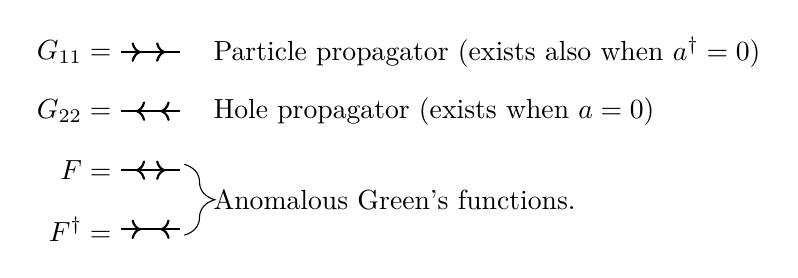
\begin{tikzpicture}[scale = 0.75]
	\node[anchor = east] (a) at (0,0) {$F^\dagger = $};
	\node[anchor = east]  at (0,1) {$F = $};
	\node[anchor = east]  at (0,2) {$G_{22} = $};
	\node[anchor = east]  at (0,3) {$G_{11} = $};
	
	\draw[->- = 0.67, thick] (0,3) -- (0.5,3);
	\draw[->- = 0.5, thick] (0.5,3) -- (1,3);
	
	\draw[->- = 0.5, thick] (0.5,2) -- (0,2);
	\draw[->- = 0.67, thick] (1,2) -- (0.5,2);
	
	\draw[->- = 0.5, thick] (0.5,1) -- (0,1);
	\draw[->- = 0.5, thick] (0.5,1)--(1,1);
	
	\draw[->- = 0.67, thick] (0,0)--(0.5,0) ;
	\draw[->- = 0.67, thick] (1,0)--(0.5,0);
	
	
	\draw[decorate,decoration={brace,amplitude=11pt, mirror},xshift=2pt,yshift=0pt]
	(1,-0.1) -- (1,1.1);
	
	
	\node[anchor = west] at (1.4, 0.5) {Anomalous Green's functions. };
	\node[anchor = west] at (1.4, 2) {Hole propagator (exists when $a = 0$)};
	\node[anchor = west] at (1.4, 3) {Particle propagator (exists also when $a^\dagger = 0$)};	
\end{tikzpicture}
	\caption{Propagators of the system}
	\label{fig:propagators}
\end{figure}
$F\sim a, F^\dagger \sim a^\dagger $.
These two functions do not exist in the normal state, since $a = a^\dagger = 0$ in this state. Now, we are able to interpret what it means to have $a \ne 0, a^\dagger \ne 0$.
Notice that 

\begin{align}
\label{eq:order_param}
\begin{split}
\ev{\varphi_\downarrow\varphi_\uparrow} &\sim a\\
\ev{\varphi_\uparrow^\dagger\varphi_\downarrow^\dagger} &\sim a^\dagger
\end{split}
\end{align}
NB! Remember: when we Hubbard-Stratonovich decoupled $S_I$, we used the terms $a^\dagger \varphi_\downarrow\varphi_\uparrow$ and $a\varphi_\uparrow^\dagger\varphi_\downarrow^\dagger$. $a,\, a^\dagger$ are pair field that are conjugated to the order parameters $\ev{\varphi_\downarrow\varphi_\uparrow}$ and $\ev{\varphi_\uparrow^\dagger\varphi_\downarrow^\dagger}$, analog to the case of a spin system in an external magnetic field. This field is a magnetic field that are conjugated to the order parameter of the spin system, which is the magnetization, $\vb{M} \sim \vb{H}$.
The order parameters of a superconductor is as in \eqref{eq:order_param}. When these are nonzero, there is a spontaneously broken symmetry of the problem. 
Returning to $\Ha$;
\begin{equation}
	\Ha = \sum_x\varphi^*\varepsilon(\grad)\varphi + V\sum_x\varphi^*\varphi\varphi^*\varphi
\end{equation}
This model has a continous symmetry
\begin{align*}
	\varphi(x) &\rightarrow \varphi(x)\e^{i\theta(x)} \\
	\Ha &\rightarrow \Ha,
\end{align*}
 which is a $U(1)$-symmetry. However, in $\ev{\varphi_\downarrow\varphi_\uparrow}$, the phases do not cancel, but instead goes to $\ev{\varphi_\downarrow\varphi_\uparrow\e^{2i\theta}}$. If this phase is completely undetermined, this average will be zero. Thus, having $\ev{\varphi_\downarrow\varphi_\uparrow}\ne 0$ must mean that $\theta$ is a known quantity, i.e. the symmetry is spontaneously broken. 
 More generally:
 
 \textit{When we assume a saddle point in a functional integral, and also assume $\Sa_\text{eff}$ is a minimum for finite values of $\ev{a}, \ev{a^\dagger}$, this is quivalent to the assumption of some spontaneous breaking of symmetry (most often).}
 
 Thus: To choose a suitable decoupling scheme, we have to chose the ``right type'' of bosons in the H-S transformations. This choice is decided by the physcis we expect. 


\subsection{The spectra $E_k$}
The consequence of the broken symmetry discussed above is a \emph{gap} in the spectrum.

$a = 0$:
% Sett inn figurer
\begin{equation}
	\Ha = \sum_{k, \sigma}\left(\varepsilon_k-\mu\right)c_{k\sigma}^\dagger c_{k\sigma}.
\end{equation}

$a \ne 0$:

\begin{equation}
	\Ha = E_0 + \sum E_k\left(\gamma_k^\dagger\gamma_k - \eta_k^\dagger\eta_k\right)
\end{equation}

$a \ne 0 \implies $ zero resistivity and Meissner effect. Superconduction.
NB: We started with a Hamiltonian defined for fermions. We then proceeded by introducing the partition function and an effective action, $\Sa_{\text{eff}}$ (the Lagrange function)
\begin{align}
\label{eq:hamilton_gauge}
\begin{split}
	\Ha\left(\varphi^*, \varphi\right)&\rightarrow \varphi^*\pdv{\varphi}{\tau} + \Ha\left(\varphi^*, \varphi\right) \\
	 &= \Sa_0 + \Sa_I.
\end{split}
\end{align}

Notice that the dynamic term, $\varphi^*\pdv{\varphi}{\tau}$, in \eqref{eq:hamilton_gauge} only acts in the fermion sector. We then H-S-decoupled $\Sa_I$
\begin{equation}
	\e^{\Sa_I } = \int\mathcal{D}a^\dagger\mathcal{D}a\,\e^{-\frac{1}{v}a^\dagger a+a\pu^\dagger\pd^\dagger + a^\dagger \pd\pu}
\end{equation}

But: We don't get any dynamic $a^\dagger\pdv{a}{\tau}$-terms. The ($a^\dagger, a$)-bosons do not exist in the Hamilton formalismm. This means that they don't have their own dynamics. It is generated by the fermions, by $\Tr\ln\mathcal{G}^{-1}$.

\subsection{Fluctuations}
% BURDE VÆRE SUBSECTION
Later we will come back to how we correct the mean field approximations to \(\Sa_{\text{eff}}[a^\dagger, a]\). We can do this by developing to Gaussian order  (2.order) in the fluctuations in the boson fields \(a^\dagger, a\), near the saddle point. A coarse structure of this will be the following. Define 

\begin{equation}
A = 
\begin{pmatrix}
\delta a^\dagger \\
\delta a
\end{pmatrix}, 
A^\dagger =
\begin{pmatrix}
\delta a & \delta a^\dagger
\end{pmatrix}
\end{equation}

\begin{align}
\Sa_{\text{eff}} &\simeq \Sa_{\text{MF}} - \sum_q A^\dagger D^{-1}(q)A \nonumber\\
\Z &\simeq \e^{\Sa_{\text{MF}}}\int\D A^\dagger\D A\e^{- \sum_q A^\dagger D^{-1}A}\nonumber  \\
\Z &= \e^{\Sa_{\text{MF}}}\e^{-\Tr\ln D^{-1}} \label{eq:partition_fluctuations}
\end{align} where $D^{-1}$ is a \(2\times 2\) matrix. A constraint (claim) to stability of the saddle point is that $D^{-1}$ have to be positive definite, i.e. it must have only positive eigenvalues. 
With $\Z = \e^{-\beta F}$  we have 

\begin{equation}
\label{eq:free_energy_fluctuations}
F = F_{\text{MF}} + \frac{1}{\beta}\Tr\ln D^{-1}.
\end{equation}
We can now correct  the mean field values for $a, a^\dagger$ by minimizing \eqref{eq:free_energy_fluctuations} with respect to $a, a^\dagger$.

\begin{equation}
\pdv{F}{a} =0 = \pdv{F_{\text{MF}}}{a} + \underbrace{\pdv{a}\left(\frac{1}{\beta}\Tr\ln D^{-1}\right)}_{\text{Correction term}}.
\end{equation}

This means that we can find the fluctuation corrections to $T_c$ etc. We expect these corrections to be significant when $T_c$ becomes large. As of October 1996', no such calculations on the fluctuations has been made.\footnote{As of 2019, it has probably been done thoroughly.}

\section{The Hubbard model $(U = \infty)$}

Consider the Hamiltonian 
\begin{equation}
\label{eq:Hamilitonian_hubbard}
\Ha = -\sum_{i,j}t_{ij}c_{i\sigma}^\dagger c_{j\sigma} + U\sum_{i}n_{i\uparrow}n_{i\downarrow} - \mu\sum_{i,\sigma}n_{i\sigma}.
\end{equation}

At \underline{$U = 0$}, the Hamiltonian \eqref{eq:Hamilitonian_hubbard} transforms to
\begin{equation}
\Ha = \sum_{k,\sigma}\left(\varepsilon_k - \mu\right)c_{k\sigma}^\dagger c_{k\sigma}
\end{equation} with nearest neighbour hopping 
\begin{equation*}
\varepsilon_k = -2t\sum_{i = 1}^d\cos k_i \equiv -2t\gamma_k
\end{equation*}

For intermediate \underline{$0<U<\infty$} we have a very complicated problem with little or nothing known. 

For \underline{$U = \infty$} the problem simplifies, but cannot be solved exact. The simplified Hamiltonian then reads 
\begin{equation}
\Ha = -\sum_{i,j,\sigma}t_{ij}c_{i\sigma}^\dagger c_{j\sigma}
\end{equation}
with an extra constraint on each lattice site; that there is a maximum of one fermion per lattice site at all times $t$.
\begin{equation*}
\sum_\sigma \hat{n}_{i\sigma}\ket{\psi} \sum_\sigma n_{i\sigma}\ket{\psi}
\end{equation*}
with
\begin{equation*}
\underline{\sum_\sigma n_{i\sigma} \le 1}
\end{equation*}
Constraints like these, i.e. constraints represented by inequalities are difficult to deal with. 

\subsection{Hubbard operators}
Before we continue,
we introduce \underline{Hubbard operators}. Consider states \(\ket{\alpha, i}\) where \(\alpha \in 0, \sigma, 2\) and \(\sigma = \uparrow, \downarrow\). These are empty, simple, or doubly occupied states. 
Next, define
\begin{equation}
\label{eq:Hubbard_operators}
X_i^{\alpha\beta} = \dyad{\alpha, i}{\beta, i}.
\end{equation}
\begin{align}
\hat{O} &= \sum_{\alpha, \beta}\ket{\alpha, i}\mel{\alpha, i}{\hat{O}}{\beta, i}\bra{\beta, i}\nonumber \\
&= \sum_{\alpha, \beta}X_i^{\alpha\beta}\mel{\alpha, i}{\hat{O}}{\beta, i} \nonumber
\end{align}

%\newtheorem{theorem}{Ex}

\begin{theorem}
\begin{align*}
c_{i\sigma} &= \sum_{\alpha, \beta}X_i^{\alpha\beta}\mel{\alpha, i}{c_{i\sigma}}{\beta, i} \\
&= X_i^{0\sigma} + X_i^{-\sigma 2} \\
c_{i\sigma}^\dagger &= X_i^{\sigma 0} + X_i^{2-\sigma}
\end{align*}
\end{theorem}

If we let $U = \infty$, we see from \eqref{eq:Hamilitonian_hubbard} that we can drop the operators involving doubly occupied states \(X_i^{-\sigma 2},X_i^{2-\sigma}\) such that we can write\footnote{Comment in the notes: `` This is valid when the doubly occupied states gets projected out of the Hilbert space''} 
\begin{align}
\label{eq:hubbard_ops_ca}
c_{i\sigma} &= X_i^{0\sigma} \\
c_{j\sigma}^\dagger &= X_j^{\sigma 0}
\end{align}
This means that the Hamiltonian in the Hubbard model can be written 
\begin{equation}
\label{eq:hubbard_ham}
\Ha = -t\sum_{i,j,\sigma}X_i^{\sigma 0}X_j^{0\sigma}
\end{equation}
Here we thus have hopping with no double-occupancy-constraint. We have restrictions on the creation and annihilation operators, but \underline{no} restriction on the Hubbard operators \(X_i^{\sigma 0}\). Unfortunately, the problem is more complicated then what it seems. The reason is that the Hubbard operators satisfy much more complicated commutation relations. By the definition \eqref{eq:Hubbard_operators}, these are

\begin{align}
\comm{X_i^{\alpha\beta}}{X_j^{\gamma\eta}}_\pm 
&= \ket{\alpha i}\braket{\beta i}{\gamma j}\bra{\eta j} \pm \ket{\gamma j}\braket{\eta j}{\alpha i}\bra{\beta i} \nonumber \\
&= \delta_{ij}\delta_{\beta\gamma}X_i^{\alpha\eta} \pm \delta_{ij}\delta_{\eta\alpha}X_j^{\gamma\beta} \nonumber\\
&= \delta_{ij}\left[\delta_{\beta\gamma}X_i^{\alpha\eta} \pm \delta_{\eta\alpha}X_i^{\gamma\beta}\right]
\end{align}

Now, we introduce canonical boson-  and fermion operators to represent $X$ by these.
\begin{align*}
X_i^{00} &= \dyad{0i} \\
&\Leftrightarrow b_i^\dagger b_i\\
X_i^{\sigma 0} &= \dyad{\sigma i}{0i} \\
&\Leftrightarrow f_{i\sigma}^\dagger b_i \\
X_i^{0\sigma} &= \dyad{0i}{\sigma i} \\
&\Leftrightarrow b_i^\dagger f_{i\sigma}\\
X_i^{\sigma\sigma'} &= \dyad{\sigma i}{\sigma' i}\\
&\Leftrightarrow f_{i\sigma}^\dagger f_{i\sigma'}
\end{align*}
Using these representations, we get the correct commutation relations for the Hubbard operators. 

\begin{align}
\label{eq:comm_rel_repr1}
\begin{split}
\comm{X_i^{0\sigma}}{X_i^{\sigma'0}}_+ &= X_i^{0\sigma}X_i^{\sigma'0} +X_i^{\sigma'0}X_i^{0\sigma}\\
&= \delta_{\sigma\sigma'}X_i^{00} + X_i^{\sigma'\sigma} \\
&= \delta_{\sigma\sigma'}b_i^\dagger b_i + f_{i\sigma}^\dagger f_{i\sigma'}
\end{split}
\end{align}
Or,using the representations directly:
\begin{align}
\label{eq:comm_rel_repr2}
\begin{split}
\comm{b_i^\dagger f_{i\sigma}}{f_{i\sigma'}^\dagger b_i}_+ &= f_{i\sigma'}^\dagger f_{i\sigma}\left(1+b_i^\dagger b_i\right) + b_i^\dagger b_i \left(\delta_{\sigma\sigma'} - f_{i\sigma'}^\dagger f_{i\sigma}\right) \\
&= \delta_{\sigma\sigma'}b_i^\dagger b_i + f_{i\sigma'}^\dagger f_{i\sigma} \\
&= \delta_{\sigma\sigma'}X_i^{00} + X_i^{\sigma'\sigma}.
\end{split}
\end{align}
We see that \eqref{eq:comm_rel_repr1} and \eqref{eq:comm_rel_repr2} are equal and thus this representation gives the correct commutation relations. We still have the completeness relation
\begin{align}
\begin{split}
1 &= \sum_\alpha \dyad{\alpha i} \\
&= X_i^{00} + \sum_\sigma X_i^{\sigma\sigma}\\
&= b_i^\dagger b_i + \sum_\sigma f_{i\sigma}^\dagger f_{i\sigma}
\end{split}
\end{align}

\subsection{Reformulating constraint}
We now return to the general problem of constraint govern by an inequality. We wish to convert this constraint to an equality, and we develop methods for solving such problems. The trick is to introduce a boson, $b_i$, which keeps track of when a lattice site $i$ is \underline{unoccupied}.

Using our previously defined Hubbard operators, we associate, using \eqref{eq:hubbard_ops_ca}, \(c_{i\sigma}^\dagger = X_i^{\sigma 0} \Leftrightarrow f_{i\sigma}^\dagger b_i\) and \(c_{i\sigma} = X_i^{0\sigma} \Leftrightarrow  b_i^\dagger f_{i\sigma}\). 

$f_{i\sigma}^\dagger$: Creation operator for a fermion on the lattice site $i$ .
$b_i$: Creation operator for an unoccupied lattice site. 
$f_{i\sigma}^\dagger f_{i\sigma}$: The number of fermions on the lattice site $i$. 

Either the site is occupied with one fermion, or the site is empty. This is expressed with the condition 
\begin{equation}
\label{eq:constraint_hubbard}
b_i^\dagger b_i + \sum_\sigma f_{i\sigma}^\dagger f_{i\sigma} = 1,
\end{equation}
which is now a leading constraint expressed with an equality. 

The Hamiltonian \eqref{eq:hubbard_ham}of the problem is written on the form 
\begin{equation}
\label{eq:hubbard_hamiltonian2}
\Ha = -\sum_{i,j,\sigma}t_{ij}f_{i\sigma}^\dagger b_i b_j^\dagger f_{j\sigma}.
\end{equation}
Equations \eqref{eq:constraint_hubbard} and \eqref{eq:hubbard_hamiltonian2} define our problem, which we are to solve. Define
\begin{equation}
Q_i \equiv   \sum_\sigma f_{i\sigma}^\dagger f_{i\sigma} + b_i^\dagger b_i
\end{equation}
such that $Q_i = 1$ is our condition. 
\underline{Abrikosovs' trick}: \footnote{Alexei Alexeyevich Abrikosov (1928-2017), awarded with the Nobel price in physics 2003}
\begin{equation}
\prod_{i,\tau}\int_{-\pi}^\pi \frac{\dd{\lambda_i}}{2\pi}\e^{-i\int_0^\beta\lambda_i(\tau)(Q_i -1)\dd{\tau}} = \prod_{i,\tau}\delta_{Q_i,1}
\end{equation}
The partition function is given by 
\begin{equation}
\Z  = \int \D\varphi^*\D\varphi\D b^*\D b \left(\prod_i\prod_\tau\delta_{Q_i,1}\right)\e^{\Sa}
\end{equation}
where the factor in parentheses ensures that the functional integral is limited to include states where the lattice sites are \underline{not} doubly occupied.

\begin{align}
\label{eq:action_hubbard}
\begin{split}
\Sa = &-\sum_{i,\sigma}\int_0^\beta \dd{\tau}\left[\underbrace{b_i^*\pdv{b_i}{\tau}}_{\text{NB!}} + \varphi_{i\sigma}^*\pdv{\varphi_{i\sigma}}{\tau} \right] \\
&+ \sum_{i,j,\sigma}\int_0^\beta\dd{\tau}\varphi_{i\sigma}^*(\tau)b_i(\tau)t_{ij}b_j^*(\tau)\varphi_{j\sigma}(\tau)
\end{split}
\end{align}

NB: Note that we now have to keep all the terms involving $b_i^*\pdv{b_i}{\tau}$. This is because the $b$-bosons also exist in the Hamilton formulation of the theory. This is an essential difference from what we had earlier because the $b$-bosons has their own intrinsic dynamics.
We rewrite \eqref{eq:action_hubbard} as
\begin{align}
\begin{split}
\Sa = &-\sum_i\int_0^\beta\dd{\tau}b_i^*\pdv{b_i}{\tau} \\
&-\sum_{i,j,\sigma}\int_0^\beta\dd{\tau} \varphi_{i\sigma}^*\left(\partial_\tau\delta_{ij} - t_{ij}b_ib_j^*\right)\varphi_{j\sigma}.
\end{split}
\end{align} 
Now introduce Abrikosov's trick
\begin{equation}
\Z  = \int \D\varphi^*\D\varphi\D b^*\D b \D \lambda\, \e^{\tilde{\Sa}}
\end{equation}
\begin{align*}
\tilde{\Sa} = &-\sum_i\int_0^\beta\dd{\tau}b_i^*(\partial_\tau + i\lambda_i)b_i + i\sum_i\int_0^\beta\lambda_i\dd{\tau} \\
&-\underbrace{\sum_{i,j,\sigma}\int_0^\beta\dd{\tau}\varphi_{i\sigma}^*\left[\delta_{ij}(\partial_\tau + i\lambda_i) - t_{ij}b_ib_j^*\right]\varphi_{j\sigma}}_{\text{Gaussian fermion sector}}
\end{align*}
Now we can integrate out the fermion sector in an exact manner!
\begin{equation}
\Z = \int\D b^\dagger\D b\D\lambda \e^{\Sa_{\text{eff}}[b^\dagger, b, \lambda]},
\end{equation}
with
\begin{align}
\begin{split}
\Sa_{\text{eff}} &= -\sum_i\int_0^\beta\dd{\tau}b_i^\dagger\left(\partial_\tau + i\lambda\right)b_i + i\sum_i\int_0^\beta\dd{\tau}\lambda_i \\
&+ \Tr\ln\mathcal{G}^{-1}
\end{split}
\end{align}

\begin{equation}
\mathcal{G}^{-1} = \left(\partial_\tau + i\lambda_i\right)\delta_{ij}-t_{ij}b_ib_i^\dagger
\end{equation}
We have thus converted a strongly correlated fermionic system to an interacting bosonic system. 
The resulting boson-theory is again too complicated for direct calculation of $\Z$. We therefore resort to the stationary point approximation.  Let $b_i = b, i\lambda_i = \lambda$ (physical explanation will follow).
\begin{equation}
\label{eq:greens_hubbard}
\mathcal{G}^{-1} = (\partial_\tau + \lambda)\delta_{ij}- |b|^2t_{ij}.
\end{equation}
To compute \eqref{eq:greens_hubbard}, we may resort to the Fourier transform of  $\mathcal{G}^{-1}$.
\begin{align*}
\mathcal{F}(\delta_{ij}) &\Rightarrow 1 \\
\mathcal{F}(t_{ij}) &\Rightarrow \tilde{\gamma}_k = 2t\underbrace{\sum_{i}\cos(k_i)}_{\gamma_k} \\
\partial_\tau &\Rightarrow -i\omega_n.
\end{align*}
Using these relations, we find 
\begin{align}
\Tr\ln\mathcal{G}^{-1} &= \frac{1}{\beta}\sum_{k,\omega_n}\ln(-i\omega_n + \varepsilon_k) \\
&= \frac{1}{\beta}\sum_{k,\omega_n}\ln(i\omega_n - \varepsilon_k),
\end{align}
\begin{equation}
\varepsilon_k = -2tb^2\sum_i\cos(k_i) + \lambda,
\end{equation}
or, if we had included the chemical potential all the way from the start,
\begin{align*}
\varepsilon_k &= -2tb^2\gamma_k-(\mu+\lambda) \\
\Sa_{\text{eff}}^{\text{MF}} &= -N\beta b^2 \lambda + N\beta \lambda+\sum_k\ln\left(1+\e^{-\beta \varepsilon_k}\right) \\
f^{\text{MF}} &= (b^2 + 1)\lambda - \frac{1}{N\beta}\sum_k\ln\left(1+\e^{-\beta\varepsilon_k}\right)
\end{align*}

\subsection{Mean-field}

\begin{align}
\mathcal{G}^{-1} &= -i\omega_n+\varepsilon_k \\
\mathcal{G}_F(k ,i\omega) &= \frac{1}{i\omega - \varepsilon_k} = -\ev{\varphi\varphi^\dagger}
\end{align}
where 
\begin{equation}
\varepsilon_k = -2tb^2\gamma_k-(\mu+\lambda).
\end{equation}

\(\mathcal{G}_F(k, i\omega):\) Green's function for a free quasi particle with renormalized band structure (lower bandwidth, correlation effect) and renormalized chemical potential. Both of these types of renormalization originate in the ``no double occupancy constraint''.

\subsection{Stationary point constraint}
(page 140)




\section[Magnetic impurities]{\texorpdfstring{Magnetic impurities in metals - \\ \null\hfill The Anderson and Kondo models}}
(page 183-> in pdf, 139-> in notes)

Imagine that we have a system defined by free, itinerant electrons, described by a conduction band with dispersion relation $\varepsilon_k$ and, for the sake of simplicity, assume that the one-particle density of state has a simple form as shown in Figure \ref{fig:dos}. The bandwidth of this system is $2D$, and the system has a Hamiltonian
\begin{equation}
	\label{eq:hamiltonian_free}
	\Ha_c = \sum_{k, \sigma}\varepsilon_k c_{k\sigma}^\dagger c_{k\sigma}.
\end{equation}

\begin{figure}[h]
	\centering
	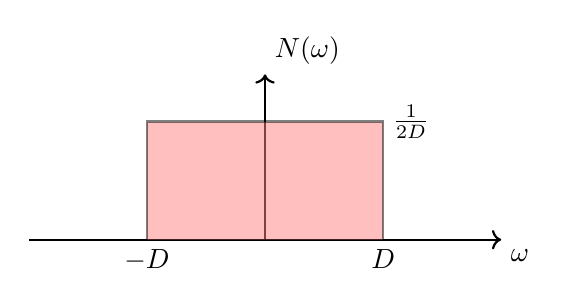
\begin{tikzpicture}[scale = 3]
	
	\draw[thick, ->] (0,1) -- (2,1);
	\draw[thick, ->] (1,1) -- (1,1.7);
	
	\draw[thick, draw = black,fill = red!50!white, opacity = 0.5] (0.5,1) rectangle (1.5,1.5);
	
	\node[anchor = north] at (0.5,1) {$-D$};
	\node[anchor = north] at (1.5,1) {$D$};
	\node[anchor = north west] at(2,1) {$\omega$};
	\node[anchor = south west] at (1,1.7){$N(\omega)$};
	\node[anchor = west] at (1.5, 1.5) {$\frac{1}{2D}$};
\end{tikzpicture}
	\caption{Density of states}
	\label{fig:dos}
\end{figure}

We will study the effect of including a magnetic impurity in the problem, where the magnetic impurity couples to the charged electrons, but is localized in space. First we consider the system with exactly one impurity. The Hamiltonian for this impurity is given by

\begin{equation}
\label{eq:hf}
	\Ha_f = E_0\sum_m f_m^\dagger f_m + U f_{\frac{1}{2}}^\dagger f_{-\frac{1}{2}}^\dagger f_{-\frac{1}{2}}f_{\frac{1}{2}},
\end{equation}

where $m$ are quantum numbers determining the z-component of the spin of the impurity. $(f_m, f_m^\dagger)$ are annihilation and creation operators for the impurity, in state $m$. $s = \frac{1}{2}: m = \pm 1$. $U$ is the Coulomb energy associated with double occupancy of the magnetic impurity. We will later assume that this is the largest energy in the system. The coupling between the charges and the localized impurity is given by
\begin{equation}
	\label{eq:interaction_term}
	\Ha_{cf}= \sum_{\vb k,\sigma,m}\left(V_{m\sigma}(\vb{k}) f_m^\dagger c_{\vb k\sigma}  + \text{h.c.}\right).
\end{equation}

In \eqref{eq:interaction_term}, $V_{m\sigma}(\vb k) $ is the matrix element transfering an electron from the impurity to the conduction band, or opposite. 
The total Hamiltonian is
\begin{equation}
	\Ha = \Ha_c + \Ha_f + \Ha_{cf}.
\end{equation}
$\Ha$ is often called the Anderson model. This model is the fundament for our understanding of heavy fermion systems. We will now use the techniques to study the effects of including a magnetic impurity in the conduction band. 
One important effect of magnetic impurities is that a metal will exhibit a minima in resistivity (see Figure \ref{fig:resistivity}).
\begin{figure}
	\centering
	\begin{tikzpicture}
    \begin{axis}[
        xmin = 0, xmax = 2,
        ymin = 0,% ymax = 1,
        axis lines = center,
        axis on top =true,
        domain = 0.1:1.6,
        %restrict y to domain=0:1,
        ylabel = $\rho(T)$,
        y label style={anchor=east},
        xlabel = $T$,
        xtick ={1},
        xticklabels={$T_K$},
        ytick style={draw=none},
        yticklabels={,,},
        samples = 100,
        %ticks = none
        ]
        
        \addplot[mark = none, draw = red!50!white, ultra thick]{1 -5*ln(x) + x^5};
        
        %\addplot[mark = none, draw = red!50!white, dashed]{1 -5*ln(x)};
        %\addplot[mark = none, draw = red!50!white, dashed]{x^5};
        
    	%\draw [thick] (axis cs:1.25,0)-- (axis cs:1.25,0.21);
    
        \node at (axis cs:0.6,5.5) {\footnotesize $\sim\ln T$};
        \node at (axis cs:1.25,6) {\footnotesize $T^5\sim $};
       	%\node[anchor = south] at (axis cs:1, 0) {$T_K = $ Kondo temperature};
        %\draw[->] (axis cs:3, 0.35) --(axis cs:4, 0.35) ;
    \end{axis}
\end{tikzpicture}
	\caption{Resistivity}
	\label{fig:resistivity}
\end{figure}
$T_K$ is only a couple of Kelvin, but the Fermi-energy is of order $10^4\mathrm{K}$. How can an energy scale this small arise when the basis is that the relevant energy scale is $\varepsilon_F \sim 10^4\mathrm{K}$? If magnetic impurities are excluded, the resistivity is uniformly decreasing. Jun Kondo found that $\rho(T) \sim -\ln T$ diverges in perturbation theory at low temperatures\footnote{Progress of Theoretical Physics, Vol. 32, No. 1, pp. 37-49}. A new problem then arises; how can we give a consistent description of low temperaturre physics, $T<<T_K$, in systems with a minima in resistivity? This problem is often referred to as the ``Kondo problem''. 

What we will do, is to see how the energy scale $T_K$, The Kondo temperature, arises, as well as to give a consistent description of the lowæ-temperature physics in metals doped with magnetic impurities, in a saddle point approxiimation.
Typical materials described by these theories are metals like aluminium and gold, doped with other rare materials. These materials are then the magnetic impurities in the problem. Rare materials: Lanthanides and actinides. Most studied: Cerium (Lanthanide) and Uranium (actinide). In the lanthanides the valence electrons are in the 4f-shell, and in actinides they are in the 5f-shell (hence $f_m^\dagger, f_m)$). Regularly studied materials are $\mathrm{CeAl_2}$ (lanthanide) and $\mathrm{UPt_3}$ (Actinide). $\mathrm{UPt_3}$ is a very odd superconductor with $T_C \sim 1\mathrm{mK}$ and a very complicated order parameter.  

Let us simplify the Anderson model;

\textbf{i)}: $U = \infty$.

Doubly occupancy of the magnetic impurities are not allowed. If there already exist a spin on the lattice site of the impurity, a conducting electron can not enter this localized orbital.

\textbf{ii)}: We assume that the coupling between $f$- and $c$-electrons are such that $m = \sigma$,  i.e. 
\begin{equation}
	V_{m\sigma}(k) =\delta_{m\sigma}V(k), 
\end{equation}
and that $V(k)$ is $k$-independent (completely localized coupling)
\begin{equation}
	V_{m\sigma}(k) = V\delta_{m\sigma}
\end{equation}
which implies
\begin{equation}
	\Ha_{cf} = V\sum_{\sigma k}\left(f_\sigma^\dagger c_{k\sigma} + h.c.\right).
\end{equation}

Thus, we have the model 
\begin{align}
	\begin{split}
	\Ha &= E_0\sum_{\sigma}f_\sigma^\dagger f_\sigma + \sum_{k,\sigma}\varepsilon_k c_{k\sigma}^\dagger c_{ck}^\dagger \\
	&= V\sum_{k,\sigma}\left[f_{\sigma}^\dagger c_{k\sigma} + h.c. \right],
	\end{split}
\end{align}

with \(\sum_mf_m^\dagger f_m \leq 1 \). It is the restiriction on the occupation number on the impurities that makes this a hard problem.

For later reference, we first solve the problem with $U = 0$.
\subsection{$U = 0$}

\begin{equation}
\Z = \int \D c^\dagger \D c\D f^\dagger \D f\e^{\Sa}
\end{equation}
\begin{equation}
\Sa = -\int\left(\sum_{k,\sigma}c_{k\sigma}^\dagger\pdv{c_{k\sigma}}{\tau} + \sum_mf_m^\dagger \pdv{f_m}{\tau} + \Ha \right)\dd{\tau}
\end{equation}

\begin{align}
\begin{split}
\Sa = &- \int_0^\beta\sum_{k,\sigma}c_{k\sigma}^\dagger\left(\partial_\tau + \varepsilon_k\right)c_{k\sigma} \dd{\tau} \\
&-\int_0^\beta\sum_\sigma f_\sigma^\dagger\left(\partial_\tau + E_0\right)f_\sigma \dd{\tau}\\
&-\int_0^\beta V\sum_{k, \sigma}\left(f_\sigma^\dagger c_{k\sigma} + h.c.\right)\dd{\tau}
\end{split}
\end{align}
\(\Z\) can be computed exactly by a linear shift og the fermion operators \((c_{k\sigma}, c_{k\sigma}^\dagger)\). Introduce \(\Gre^{-1}= \partial_\tau + \varepsilon_k\). Consider now the quantity
\begin{align}
\label{eq:temp_derivation}
	&\sum_{k, \sigma}\left[c_{k\sigma}^\dagger \Gre^{-1}c_{k\sigma}+ Vf_{\sigma}^\dagger c_{k\sigma} + Vc_{k\sigma}^\dagger f_\sigma\right] \nonumber\\
	&= \sum_{k\sigma}\left(c_{k\sigma}^\dagger + Vf_\sigma^\dagger \Gre\right)\Gre^{-1}\left(c_{k\sigma} + V\Gre f_\sigma\right) -\sum_{k,\sigma}V^2f_\sigma^\dagger \Gre f_\sigma \nonumber\\
	&=\sum_{k\sigma}\tilde{c}_{k\sigma}^\dagger \Gre^{-1}\tilde{c}_{k\sigma} - \sum_\sigma f_\sigma^\dagger\left(\sum_k V^2\Gre\right)f_\sigma.
\end{align}
Inserting \eqref{eq:temp_derivation} into the action, we get
\begin{equation}
\label{eq:action_magnetic}
	S =-\sum_{k,\sigma}\tilde{c}_{k\sigma}^\dagger \Gre^{-1}\tilde{c}_{k\sigma}-\sum_\sigma f_\sigma^\dagger\left(\partial_\tau + E_0 - V^2\sum_k\frac{1}{\partial_\tau + \varepsilon_k}\right)f_\sigma.
\end{equation}
As we can see in \eqref{eq:action_magnetic}, the action is quadratic in the $c$- and $f$- sectors.

\begin{equation}
	\Z = \int\D\tilde{c}^\dagger\D\tilde{c}\D f^\dagger \D f\, \e^{\Sa}= \Z_c\cdot\Z_f,
\end{equation}
where 
\begin{align}
	\Z_c &= \e^{\Tr\ln \left(\Gre^{-1}\right)} & \Z_f&= \e^{\Tr\ln\left(\mathcal{G}_f^{-1}\right)}\\
	\label{eq:fermi_propagator}
	\Gre^{-1} &= \partial_\tau + \varepsilon_k &
	\mathcal{G}_f^{-1} &= \partial_\tau + E_0 -V^2\sum_k \frac{1}{\partial_\tau + \varepsilon_k}.
\end{align}

$\Z_c$ is the partition function for free electron gas, and $\Z_f$ is the partition function for the impurities, coupled to a free electron gas.

we have already considered
\begin{equation}
\label{eq:free_energy_non_interacting}
	\Tr\ln\Gre^{-1} = \sum_{k,\sigma}\ln\left(1 + \e^{-\beta\varepsilon_k}\right).
\end{equation}
\eqref{eq:free_energy_non_interacting} is the free energy for non-interacting electron gas, as we have seen earlier (see the derivation of \eqref{eq:partition_free_electron}).

\begin{equation}
\label{eq:trace_impurities}
	\Tr\ln\left(\mathcal{G}_f^{-1}\right) = \sum_\sigma\sum_{\omega_n}\ln\left(-i\omega_n + E_0 +V^2\sum_k \frac{1}{i\omega_n - \varepsilon_k}\right)
\end{equation}

Consider now the last $k$-summation in \eqref{eq:trace_impurities}.
\begin{align}
\label{eq:k_sum}
\begin{split}
	\sum_k\frac{1}{i\omega_n - \varepsilon_k} &= \frac{1}{2D}\int_{-D}^D\dd{\varepsilon}\frac{1}{i\omega_n - \varepsilon} \\
	&= \frac{1}{2D}\ln\left(\frac{D+i\omega_n}{-D + i\omega_n}\right)\\
	&=-\frac{1}{2D}\ln\left(\frac{\omega_n+iD}{\omega_n-iD}\right)
\end{split}
\end{align}
This is evaluated as
\begin{equation}
	\ln\left(\frac{z}{z^*}\right) = \ln\left(\frac{|z|e^{i\varphi}}{|z|\e^{-i\varphi}}\right) = 2i\varphi.
\end{equation}
Here, $\varphi = \tan[-1](\frac{D}{\omega_n}) \simeq \frac{\pi}{2}\mathrm{sgn}(\omega_n)$ as $T\rightarrow 0$.
This implies that we can write the $k$-sum in \eqref{eq:k_sum} as
\begin{align}
	\sum_k\frac{1}{i\omega_n - \varepsilon_k} &\simeq -i\frac{\pi\cdot 2}{2\cdot 2D}\mathrm{sgn}(\omega_n)\\
	&= -i\pi\rho_0\mathrm{sgn}(\omega_n)
\end{align}
where we introduced $\rho_0 = \flatfrac{1}{2D}$. Define $\Delta_0 \equiv \pi\rho_0 V^2$. Going back to \eqref{eq:trace_impurities}, we now have
\begin{equation}
	\sum_k\frac{1}{i\omega_n - \varepsilon_k} = \sum_\sigma\sum_{\omega_n}\ln\left(-i\omega + E_0 - i\Delta_0 \mathrm{sgn}(\omega_n)\right).
\end{equation}
Following the same methods as we have seen earlier, we have
\begin{align}
	\sum_{\omega_n}\dots &= \frac{-\beta}{2\pi i}\oint\dd{z}f(z)\ln(-z+E_0-i\Delta_0\mathrm{sgn}(\Im{z}))\nonumber\\
	&= -\frac{\beta}{2\pi i }\int_{-D}^{D}\dd{\varepsilon}f(\varepsilon)\left[\ln(-\varepsilon + E_0- i\Delta_0) - \ln(-\varepsilon + E_0 + i\Delta_0)\right] \nonumber\\
	\label{eq:action_derivation}
	&= \frac{\beta}{\pi}\int_{-D}^D\dd{\varepsilon}f(\varepsilon)\tan[-1](\frac{\Delta_0}{E_0 - \varepsilon}).
\end{align}
Thus, after the spin-summation, our total action is
\begin{equation}
\label{eq:action_impurities}
	\Sa = -2\sum_k\ln\left(1 + \e^{-\beta\varepsilon_k}\right) + \frac{2\beta}{\pi}\int_{-D}^D\dd{\varepsilon}f(\varepsilon)\tan[-1](\frac{\Delta_0}{E_0 - \varepsilon}).
\end{equation}
$\Sa$ describes a free electron gas, plus a scattering resonance at the energy $E_0$ caused by the coupling between  $f$- and $c$-electrons. Notice that if $|E_0| >> D$ ,the second term in \eqref{eq:action_impurities} can be neglected. The impurities are far from the conduction band, and does not matter. When $U = \infty$, this will drastically change this result, as we shall now see.

NB! The Green's functions:
\begin{align*}
	-\ev{ff^\dagger} &= -\left(\partial_\tau + E_0 - V^2 \sum_k\frac{1}{\partial_\tau + \varepsilon_k}\right)^{-1}\\
	&\rightarrow \left(i\omega_n-E_0 + V^2\sum_k \frac{1}{i\omega_n - \varepsilon_k}\right)^{-1} \\
	-\ev{\tilde{c}\tilde{c}^\dagger} &= -\frac{1}{\partial_\tau + \varepsilon_k} \\
	&\rightarrow \frac{1}{i\omega_n-\varepsilon_k},
\end{align*}
but the $\tilde{c}$-``electrons'' are \underline{not} physical electrons. We defined them as $\tilde{c} = c+V\Gre f_\sigma \Rightarrow c = \tilde{c} - V\Gre f_\sigma$.
Then, the conducting-electron-propagator is modified;
\begin{align*}
	-\ev{cc^\dagger} &= -\left[\ev{(\tilde{c}-V\Gre f_\sigma)(\tilde{c}^\dagger - V\Gre f_\sigma^\dagger)}\right]\\
	&= -\Gre + V\Gre\ev{\tilde{c}f^\dagger} + V\Gre\ev{f\tilde{c}^\dagger} - V^2\Gre\ev{ff^\dagger}\Gre
\end{align*}

The propagator for the conducting electrons is then
\begin{equation}
	\mathcal{G}(\partial_\tau, \varepsilon_k) = -\left[\Gre(\partial_\tau, \varepsilon_k) + V^2\Gre(\partial_\tau, \varepsilon_k)\mathcal{G}_f(\partial_\tau)\Gre(\partial_\tau, \varepsilon_k)\right]
\end{equation}
\subsection{$U = \infty$}
Remember that $U$ is the energy of the Coloumb interaction from double occupancy of the impurities defined in \eqref{eq:hf}.
\begin{equation}
	\Ha = E_0\sum_\sigma F_\sigma^\dagger F_\sigma + \sum_{k,\sigma}\varepsilon_k c_{k\sigma}^\dagger c_{k\sigma} + V\sum_{k,\sigma}\left(F_\sigma^\dagger c_{k\sigma} + c_{k\sigma}^\dagger F_\sigma\right)
\end{equation}
Our constraint reads
\begin{equation}
\sum_m F_m^\dagger F_m \le 1,
\end{equation}
i.e. we have \underline{no} double occupancy. As we did for the Hubbard model at $U = \infty$, wee introduce $b$-bosons.
\begin{align*}
	F_m^\dagger &= f_m^\dagger b \\
	F_m &= f_mb^\dagger\\
	\sum_m &f_m^\dagger f_m + b^\dagger b = 1
\end{align*}
$F_m, F_m^\dagger$ are Hubbard operators, and does not satisfy simple commutation relations. When this restriction is satisfied, we have
\begin{equation}
	\Ha = E_0\sum_m f_m^\dagger f_m + \sum_{k,\sigma}\varepsilon_k c_{k\sigma}^\dagger c_{k\sigma} + V\sum_{k,\sigma}\left(f_\sigma^\dagger bc_{k\sigma} + c_{k\sigma}^\dagger b^\dagger f_\sigma\right)
\end{equation}
with the restriction 
\begin{equation}
	\sum_m f_m^\dagger f_m + b^\dagger b = 1 \equiv Q.
\end{equation}
As we did for  $U=\infty$ Hubbard:
\begin{align}
	\Z &= \int\mathcal{D}c^\dagger\mathcal{D}c\mathcal{D}f^\dagger\mathcal{D}f\mathcal{D}b^\dagger\mathcal{D}b\,\e^{\Sa}\delta_{Q,1} \\
	\begin{split}
	\Sa &= -\sum_m\int_0^\beta \dd{\tau} f_m^\dagger\left(\partial_\tau + E_0\right)f_m - \sum_{k,\sigma}\int_0^\beta \dd{\tau} c_{k\sigma}\left(\partial_\tau + \varepsilon_k\right) c_{k\sigma}) \\
	&\quad -\int_0^\beta \dd{\tau}b^\dagger\partial_\tau b - V\sum_{k, \sigma}\int_0^\beta \dd{\tau}\left(c_{k\sigma}^\dagger b^\dagger f_\sigma + f_\sigma^\dagger b c_{k\sigma}\right).
	\end{split}
\end{align}
Again, we use Abrikosov's trick, that for each value of $\tau$ use that
\begin{align}
	\delta_{Q,1} &= \int_{-\pi}^\pi \frac{\dd{\lambda}}{2\pi}\e^{-i\lambda(Q-1)} \\
	\Rightarrow \Z &= \int_{-\pi}^\pi \frac{\dd{\lambda}}{2\pi}\int\mathcal{D}c^\dagger\mathcal{D}c\mathcal{D}f^\dagger\mathcal{D}f\mathcal{D}b^\dagger\mathcal{D}b\,\e^{\tilde{\Sa}} \\
	\begin{split}
		\tilde{\Sa} &= -\sum_m\int_0^\beta \dd{\tau} f_m^\dagger\left(\partial_\tau + E_0 + i\lambda\right)f_m - \sum_{k,\sigma}\int_0^\beta \dd{\tau} c_{k\sigma}\left(\partial_\tau + \varepsilon_k\right) c_{k\sigma}) \\
		&\quad -\int_0^\beta \dd{\tau}b^\dagger\left(\partial_\tau + i\lambda\right) b - V\sum_{k, \sigma}\int_0^\beta \dd{\tau}\left(c_{k\sigma}^\dagger b^\dagger f_\sigma + f_\sigma^\dagger b c_{k\sigma}\right) + i\int_{0}^\beta\dd{\tau}\lambda  
	\end{split}
\end{align}
Again we introduce $\Gre = \partial_\tau + \varepsilon_k$, and make a shift of the $c$-fields:
\begin{align*}
	\sum_{k\sigma}&\left[c_{k\sigma}^\dagger \Gre^{-1}c_{k\sigma} + V\left(c_{k\sigma}^\dagger b^\dagger f_\sigma + f_\sigma^\dagger bc_{k\sigma}\right)\right]\\
	&=\sum_{k,\sigma}\underbrace{\left(c_{k\sigma}^\dagger + Vf_{\sigma}^\dagger b\Gre\right)}_{\tilde{c}^\dagger}\Gre^{-1}\left(c_{k\sigma} + V\Gre b^\dagger f_\sigma\right) \\
	&\quad - V^2\sum_\sigma f_\sigma^\dagger b\left(\sum_k\Gre\right)b^\dagger f_\sigma
\end{align*}
Now, do the functional integrals $\int\mathcal{D}\tilde{c}^\dagger\mathcal{D}\tilde{c}$ such that $\Z = \Z_0\cdot\tilde{\Z}$ with 
\begin{equation*}
\Z_0 = \e^{\Tr\ln\Gre^{-1}}
\end{equation*}
and
\begin{equation*}
	\tilde{\Z} = \int_{-\pi}^\pi \frac{\dd{\lambda}}{2\pi}\int\mathcal{D}f^\dagger\mathcal{D}f\mathcal{D}b^\dagger\mathcal{D}b\,\e^{\Sa_{\text{eff}}},
\end{equation*}
where 
\begin{align*}
\Sa_{\text{eff}} = \int_0^\beta\dd{\tau}[-b^\dagger\left(\partial_\tau + i\lambda\right)b &- \sum_m f_m^\dagger\left(\partial_\tau + E_0 + i\lambda\right)f_m\\
&+ \sum_m f_m^\dagger V^2 b\left(\sum_k\Gre\right)b^\dagger f_m \\
&+i\lambda]
\end{align*}
We can now do the $\int\mathcal{D}f^\dagger\mathcal{D}f$-integration:
\begin{equation}
	\tilde{\Z} = \int_{-\pi}^\pi\frac{\dd{\lambda}}{2\pi}\int\mathcal{D}b^\dagger\mathcal{D}b\,\e^{\tilde{\Sa}_{\text{eff}}[b^\dagger, b, \lambda]}.
\end{equation}
The theory is now bosonized, with
\begin{align}
\tilde{\Sa}_{\text{eff}}[b^\dagger, b, \lambda] &= -\int_0^\beta \dd{\tau}\left(b^\dagger\left(\partial_\tau + i\lambda\right)b + i\lambda\right) + \Tr\ln(\mathcal{G}_f^{-1}[b^\dagger, b, \lambda]) \\
\mathcal{G}_f^{-1} &= \partial_\tau + E_0 + i\lambda-V^2b^\dagger\left(\sum_k\frac{1}{\partial_\tau + \varepsilon_k}\right)b
\end{align}
Remembering the results \eqref{eq:fermi_propagator} for $U=0$, we see that $U=\infty$ has two effects:
\begin{enumerate}[i]
	\item Shift of $E_0$
	\item Renormalized hybridisation
\end{enumerate} 
Again, the resulting effective action is to complicated to be calculated exactly. Let us therefore introduce a saddle point approximation by
\begin{align*}
b(\tau)&= b\\
i\lambda &=\lambda.
\end{align*}

\begin{align}
	\tilde{\Sa}_{\text{eff}} &= -\beta\lambda(b^2-1) + \Tr\ln\left(\partial_\tau + E_0 + \lambda-V^2b^2\sum_k\Gre\right)\nonumber \\
	&=-\beta\lambda(b^2-1) + \sum_\sigma\sum_{\omega_n}\ln\left(-i\omega_n + \varepsilon_f + s_0^2\sum_k\frac{1}{i\omega_n-\varepsilon_k}\right)\nonumber \\
	&= -\beta\lambda(b^2-1) + 2\sum_{\omega_n}\ln\left(-\omega_n + \varepsilon_f -i\Delta\mathrm{sgn}(\omega_n)\right)\nonumber \\
	\label{eq:effective_action}
	&= -\beta\lambda(b^2-1) + 2\beta\int_{-D}^D \frac{\dd{\varepsilon}}{\pi}f(\varepsilon)\tan[-1](\frac{\Delta}{\varepsilon_f - \varepsilon}),
\end{align}
where we introduced $s_0 \equiv bV, \Delta \equiv \pi\rho_0s_0^2$ and followed the same derivation as \eqref{eq:action_derivation} with the appropriate changes.
If we compare \eqref{eq:effective_action} with the effective action from the $U = 0$ -case,
\begin{equation}
	\Sa_{\text{eff}, U=0}  = 2\beta\int_{-D}^D\frac{\dd{\varepsilon}}{\pi}f(\varepsilon)\tan[-1](\frac{\Delta_0}{E_0 - \varepsilon}),
\end{equation}
we have for $U=\infty$ a shift in the scattering resonance at $\varepsilon_f = E_0 + \lambda$. As we will now see, $\varepsilon_f$ is ``nailed'' to the Fermi-level, such that even if $E_0$ is far outside the conduction band, $\varepsilon_f$ is practically on the Fermi level. Thus, impurities always affect the physics at the Fermi level. This permanent nailing is the origin of the Kondo-effect and heavy-fermion behaviour. \textbf{This is thus a correlation effect.}

\section{Anderson lattice-model and Heavy Fermion systems}

Assume a metal where we have introduced so many magnetic impurities that we cannon treat them as isolated impurities anymore. We are therefore looking at a itinerant electron-system, coupled to a lattice of Kondo-type impurities, similar to the impurities in the last section. The system is then described by the Anderson lattice-model: 

\begin{align*}
    H = \sum_{k\sigma} \ep_k \cd_{k\sigma}c_{k\sigma} + E_0 \sum_{i\sigma} \Fd_{i\sigma} F_{i\sigma} + U\sum_i \Fd_{i \uparrow} F_{i \uparrow} \Fd_{i \downarrow} F_{i \downarrow} \\ 
    + \sum_{ik\sigma} V_{k\sigma i} \left(\cd_{k\sigma}F_{i\sigma} + \Fd_{i\sigma}c_{k\sigma}\right)
\end{align*}

this is also a complicated problem, due to the $U$-term. We set $U = \infty$, as we did before, which means no-double occupancy constraint on each lattice site $i$. The number of lattice sites are constant, whereas the number of occupants can vary. We define new fermionic and bosonic operators, similarly to what we did before 

\begin{align*}
    \Fd_{i\sigma} = \fd_{i\sigma}b_i \\ 
    F_{i\sigma} = f_{i\sigma} \bd_i. 
\end{align*}

We therefore have an extra boson-field, $b_i$, similar to what we had in the impurity problem, but now for each lattice site $i$. From this, we get 

\begin{align*}
    \sum_\sigma \Fd_{i\sigma} F_{i\sigma} \leq 1 \\
    \implies Q_i \equiv \sum_\sigma \fd_{i\sigma}f_{i\sigma} + \bd_i  b_i = 1. 
\end{align*}

The partition function for $U = \infty$: 

\begin{align*}
    Z = \int \D \cd \D c \D \fd \D f \D \bd \D b \left(\prod_{i\tau} \delta_{Q_i, 1} \right) \e^S \\ 
    S = -\sum_{i\sigma} \int_{0}^{\beta} \dd \tau \left[ \bd_i \pdv{b_i}{\tau} + \fd_{i\sigma}(\partial_\tau + E_0)f_{i\sigma} \right] - \sum_{k\sigma} \int_{0}^{\beta} \dd \tau \cd_{k\sigma}(\partial_\tau + \ep_k)c_{k\sigma} \\ 
    - \sum_{k\sigma i} \int_{0}^{\beta} \dd \tau V_{k\sigma i}\left( \cd_{k\sigma} \bd_i f_{i\sigma} + \fd_{i\sigma}c_{k\sigma} b_i \right) 
\end{align*}

where we have imposed the constraint on both imaginary time $\tau$ and the lattice points $i$. 

\begin{align*}
    \prod_{i\tau} \delta_{Q_i, 1} = \prod_{i\tau} \int_{-\pi}^{\pi} \frac{\dd \lambda_i}{2\pi}\e^{-i\sum_i  \int_{0}^{\beta} \dd \tau \lambda_i(Q_i - 1) }.
\end{align*}


Thus we get, as in the impurity problem, an un-constrained partition function, 
\begin{align*}
    Z = \int \D \cd \D c \D \fd \D f \D \bd \D b \D \lambda \e^{\Tilde{S}} \\ 
    \Tilde{S} = -\sum_{i\sigma} \int_{0}^{\beta} \dd \tau \left[ \bd_i \pdv{b_i}{\tau} + \fd_{i\sigma}(\partial_\tau + E_0)f_{i\sigma} \right] - \sum_{k\sigma} \int_{0}^{\beta} \dd \tau \cd_{k\sigma}(\partial_\tau + \ep_k)c_{k\sigma} \\ 
    - \sum_{k\sigma i} \int_{0}^{\beta} \dd \tau V_{k\sigma i}\left( \cd_{k\sigma} \bd_i f_{i\sigma} + \fd_{i\sigma}c_{k\sigma} b_i \right) - \sum_i \int_{0}^{\beta} \dd \tau i\lambda_i \left(\sum_\sigma \fd_{i\sigma}f_{i\sigma} + \bd_i  b_i - 1\right) \\
    = \sum_i \int_{0}^{\beta} \dd \tau i\lambda_i -\sum_{i\sigma} \int_{0}^{\beta} \dd \tau \left[ \bd_i (\partial_\tau + i\lambda_i)b_i  + \fd_{i\sigma}(\partial_\tau + E_0 + i\lambda_i)f_{i\sigma} \right]  \\- \sum_{k\sigma} \int_{0}^{\beta} \dd \tau \cd_{k\sigma}(\partial_\tau + \ep_k)c_{k\sigma}  
    - \sum_{k\sigma i} \int_{0}^{\beta} \dd \tau V_{k\sigma i}\left( \cd_{k\sigma} \bd_i f_{i\sigma} + \fd_{i\sigma}c_{k\sigma} b_i \right).
\end{align*}

Mean field: 

\begin{align*}
    i\lambda_i \to \lambda \quad \quad b_i \to b \quad \quad E_o + i\lambda \to E_0 + \lambda \equiv \ep_f 
\end{align*}

The the action becomes 

\begin{align*}
    \Tilde{S} = N\beta\lambda - N\beta \lambda b^2 - \sum_{i\sigma} \int_{0}^{\beta} \dd \tau \fd_{i\sigma}(\partial_\tau + \ep_f)f_{i\sigma} - \sum_{k\sigma} \int_{0}^{\beta} \dd \tau \cd_{k\sigma}(\partial_\tau + \ep_k)c_{k\sigma} \\ 
    - \sum_{k\sigma i} \int_{0}^{\beta} \dd \tau  V_{k\sigma i}b\left( \cd_{k\sigma}f_{i\sigma} + \fd_{i\sigma}c_{k\sigma}\right), 
\end{align*}

where $N$ is the volume, i.e. the number of impurity lattice sites, of the system. Now we approximate the coupling term and Fourier transform the k-part of the $f$-sector 

\begin{align*}
    \sum_{i\sigma} \int_{0}^{\beta} \dd \tau \fd_{i\sigma}(\partial_\tau + \ep_f)f_{i\sigma} \to \sum_{k\sigma} \int_{0}^{\beta} \dd \tau \fd_{k\sigma}(\partial_\tau + \ep_f)f_{k\sigma} \\
    - \sum_{k\sigma i} \int_{0}^{\beta} \dd \tau V_{k\sigma i}b\left( \cd_{k\sigma}f_{i\sigma} + \fd_{i\sigma}c_{k\sigma}\right) \to - \sum_{k\sigma} \int_{0}^{\beta} \dd \tau Vb\left( \cd_{k\sigma}f_{k\sigma} + \fd_{k\sigma}c_{k\sigma}\right). 
\end{align*}

When we write the model like this, it is essentially a Fourier transformed real-space model with unit cells consisting of $c-$ and $f-$electron orbitals. The $c-$electrons can jump, whereas the $f-$ electrons cannot, since they are dispersion-less. They become mobile, since they are coupled to the $c-$electrons via the matrix element $V$. 
\begin{align*}
    \sum_{ij\sigma} t_{cc}^{ij} \cd_{i\sigma} c_{j\sigma} \to \sum_{k\sigma} \ep_k \cd_{k\sigma} c_{k\sigma} \\ 
    E_0 \sum_i \Fd_{i\sigma} F_{i\sigma} \to E_0 \sum_k \Fd_{k\sigma} F_{k\sigma} \\
    V \sum_i \left( \cd_i F_i + \Fd_i c_i \right) \to V\sum_{k\sigma} \left( \cd_{k\sigma} F_{k\sigma} + \Fd_{k\sigma} c_{k\sigma} \right)
\end{align*}

and there are as many lattice sites for the electrons as there are for the impurities. Then we get, in mean field theory \\

\begin{align*}
    Z = \e^{-N\beta \lambda (b^2 - 1)} \int \D \psi^\dagger \D \psi \e^{S_{MF}} \\ 
    S_{MF} = -\sum_{k\sigma} \int_{0}^{\beta} \dd \tau \psi^\dagger_{k\sigma}A\psi_{k\sigma} \\ 
    \psi_{k\sigma} = \begin{pmatrix} c_{k\sigma} \\ f_{k\sigma} \end{pmatrix} \\
    A = \begin{pmatrix} \partial_\tau + \ep_k && Vb \\
    Vb && \partial_\tau + \ep_f \end{pmatrix} 
\end{align*}

\begin{align*}
    Z = \e^{-N\beta \lambda (b^2 - 1)} \e^{\Tr\ln A} 
\end{align*} 
\begin{align*}
    \Tr \ln A = \sum_{k\sigma} \int_{0}^{\beta} \dd \tau \tr \ln \begin{pmatrix} \partial_\tau + \ep_k && Vb \\
    Vb && \partial_\tau + \ep_f \end{pmatrix} \\ 
    = \frac{1}{\beta}\sum_{\omega_n}\sum_{k \sigma} \int_{0}^{\beta} \dd \tau \tr \ln \begin{pmatrix} -i\omega_n + \ep_k && Vb \\
    Vb && -i\omega_n + \ep_f \end{pmatrix} \\
    = \sum_{\omega_n}\sum_{k \sigma} \ln(i\omega_n - E_k^+)(i\omega_n - E_k^-) = 2\sum_k \ln\left[\left(1 + \e^{-\beta E_k^+}\right)\left(1 + \e^{-\beta E_k^-}\right)\right] \\
    E_k^{\pm} = \frac{1}{2}\left( \ep_k + \ep_f \pm \sqrt{(\ep_k - \ep_f)^2 +4V^2b^2} \right) \\
    f = N\lambda (b^2 - 1) - \frac{2}{\beta} \sum_k \left[ \ln \left(1 + \e^{-\beta E_k^+}\right)\ \ln\left(1 + \e^{-\beta E_k^-}\right) \right] 
\end{align*}

\begin{figure}
    \centering
    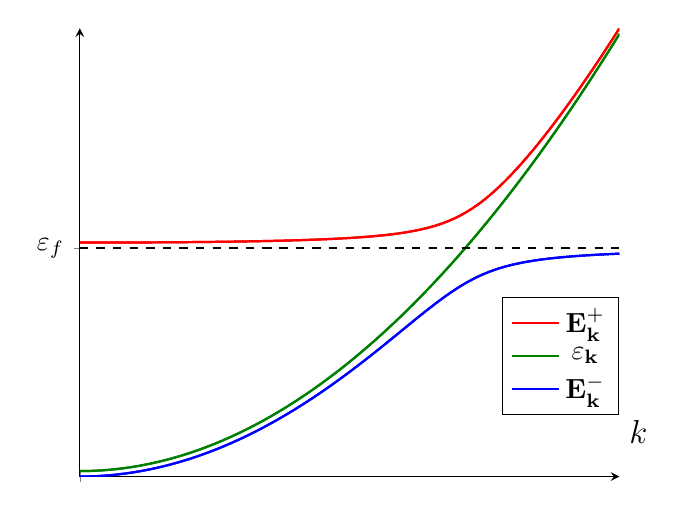
\begin{tikzpicture}
\begin{axis}[
    legend style={at={(1,0.4)}},
    ytick = {1},
    yticklabels = {$\varepsilon_f$},
    xtick = {0},
    xticklabels ={,,},
    xlabel = \large $k$,
    axis lines = left,
    x label style={at={(axis description cs:1,0.1)}, anchor = west},
    %y label style={at={(axis description cs:0.15,1)},rotate=-90,anchor=south},
    %xlabel = $x$,
    %sylabel = {$f(x)$},
]
%Below the red parabola is defined
\addplot [
    thick,
    domain=0:1.4, 
    samples=100, 
    color=red,
]{1/2 * (1 + x^2 + sqrt((x^2 - 1)^2 + 0.1))};


\addplot [
    thick,
    domain=0:1.4, 
    samples=100, 
    color=green!50!black,
]{x^2};

%Here the blue parabloa is defined
\addplot [
    thick,
    domain=0:1.4, 
    samples=100, 
    color=blue,
    ]{1/2 * (1 + x^2 - sqrt((x^2 - 1)^2 + 0.1))};


\addplot[
    thick,
    domain = 0:1.4,
    samples = 100,
    dashed
    ]{1};

\addlegendentry{$\mathbf{E_k^+}$}
\addlegendentry{$\mathbf{\varepsilon_k}$}
\addlegendentry{$\mathbf{E_k^-}$}
\end{axis}
\end{tikzpicture}
    \caption{How the dispersion relation changes when $V \ne 0$. NB: All the energy levels relative the Fermi-level.}
    \label{fig:my_label}
\end{figure}


Again this has the form of an electron gas plus a purely bosonic contribution. \\ 

We see that the dispersion relations close to the renormalized impurity-surface $(\ep_f)$ are very flat. This implies that the quasi-particles have a large effective mass. \\

\begin{align*}
    Z = Z_b \cdot Z_f \\
    Z_f = \int \D \psi^\dagger \D \psi e^S \\
    S = -\sum_{k\sigma} \int_{0}^{\beta} \dd \tau \psi^\dagger_{k\sigma} A \psi_{k\sigma} 
\end{align*}

This partition function is an effective free-fermion theory with the Hamilton-operator 

\begin{align*}
    H = \sum_{k\sigma} \psi_{k\sigma}^\dagger \begin{pmatrix} \ep_k && Vb \\
    Vb && \ep_f \end{pmatrix} \psi_{k\sigma} \\
    S = - \int_{0}^{\beta} \dd \tau \left[ \sum_{k\sigma} \psi_{k\sigma}^\dagger \pdv{\psi_{k\sigma}^\dagger}{\tau} + \psi_{k\sigma}^\dagger H \psi_{k\sigma} \right] \\ = \sum_{k\sigma} \varphi_{k\sigma}^\dagger \pdv{\varphi_{k\sigma}^\dagger}{\tau} + \varphi_{k\sigma}^\dagger D \varphi_{k\sigma} \\
    H = \sum_{k\sigma} E_k^+\varphi_{k\sigma, +}^{\dagger} \varphi_{k\sigma, +} + E_k^- \varphi_{k\sigma, -}^\dagger \varphi_{k\sigma, -} 
\end{align*}

\begin{align*}
    \varphi_{k\sigma} = \begin{pmatrix} \varphi_{k\sigma, +}  \\ \varphi_{k\sigma, -} \end{pmatrix} \quad D = \begin{pmatrix} E_k^+ && 0 \\ 0 && E_k^- \end{pmatrix} 
    %Karl p. 222
\end{align*}

Where we have diagonalized the Hamiltonian. Even when $U \to \infty$, the system is a renormalized free electron gas, maybe with heavy electrons! \\ 

In the last section, we proved that $\ep_f$ was nailed to the Fermi-surface

\begin{align*}
    \ep_f = D \e^{-\frac{\pi \abs{E_0}}{2\Delta_0}} \quad \Delta_0 = \pi \rho_0 V^2. 
\end{align*}

Is this the case in this lattice model? To answer this question, we must solve the stationary point equation. \\

The physics of the system is determined at the Fermi-surface, or very near. If $\ep_f$ is nailed to the Fermi-surface in this case as well, the low-energy excitations (i.e. most important fluctuations) will have a large effective mass: $E_k^\pm$ is flat near $\ep_f$. We get a heavy-fermion system from correlation effects, because $\ep_f \approx \ep_F$ when $U$ is large. \\

Before moving on to the stationary point condition, we will have a look at the propagators of the system. \\ 

Fermion propagator: 

\begin{align*}
    \psi_{k\sigma} = \begin{pmatrix} c_{k\sigma} \\ f_{k\sigma} \end{pmatrix} \\ 
    G(\tau, \ep_k, \ep_f) = -\expval{\psi_{k\sigma} \psi_{k\sigma}^\dagger} \\ 
    G^{-1}(\tau, \ep_k, \ep_f) = -A = - \begin{pmatrix} \partial_\tau +\ep_k && Vb \\ Vb && \partial_\tau + \ep_f \end{pmatrix} \\ 
    G^{-1}(k, i\omega_n) = - \begin{pmatrix} -i\omega_n +\ep_k && Vb \\ Vb && -i\omega_n + \ep_f \end{pmatrix} \\
    G(k, i\omega_n) = \frac{1}{\det G^{-1}} \begin{pmatrix} i\omega_n - \ep_k && Vb \\ Vb && i\omega_n - \ep_f \end{pmatrix}
\end{align*}

\begin{align*}
    \det G^{-1} = (i\omega_n - \ep_k)(i\omega_n - \ep_f) - s_0^2 = (i\omega_n - E_k^+)(i\omega_n - E_k^-) \\ 
    E_k^\pm = \frac{1}{2}\left(\ep_k + \ep_f \pm \sqrt{(\ep_k - \ep_f)^2 + 4s_0^2}\right)
\end{align*}

\begin{align*}
    G_{cc}(k,i\omega_n) = -\expval{c_{k\sigma} c_{k\sigma}^\dagger} = \frac{i\omega_n - \ep_f}{(i\omega_n - E_k^+)(i\omega_n - E_k^-)} \\ 
    G_{ff}(k,i\omega_n) = -\expval{f_{k\sigma} f_{k\sigma}^\dagger} = \frac{i\omega_n - \ep_k}{(i\omega_n - E_k^+)(i\omega_n - E_k^-)}
\end{align*}

\begin{align*}
    G_{cf} = G_{fc} = -\expval{c_{k\sigma} f_{k\sigma}^\dagger} = \frac{s_0}{(i\omega_n - E_k^+)(i\omega_n - E_k^-)} = 0 \quad (V = 0).
\end{align*}

When the hybridization term is $0$, the vertices connecting $c-$ and $f-$field are $0$, and hence the probability of a $c-$fermion changing to a $f-$fermion is 0. \\ 

$V = 0$: 

\begin{align*}
    G_{cc}(k,i\omega_n) = -\expval{c_{k\sigma} c_{k\sigma}^\dagger} = \frac{i\omega_n - \ep_f}{(i\omega_n - \ep_k)(i\omega_n - \ep_f)} = \frac{1}{i\omega_n - \ep_k} \\ 
    G_{ff}(k,i\omega_n) = -\expval{f_{k\sigma} f_{k\sigma}^\dagger} = \frac{i\omega_n - \ep_k}{(i\omega_n - \ep_k)(i\omega_n - \ep_f)} = \frac{1}{i\omega_n - \ep_f}
\end{align*}

In this case, the $f-$fermions are dispersionless, which means that they are localized, as expected. The effect of $U$ is only present in $G_{ff}$: $E_0 \to \ep_f$. We can write these propagators on Fermi-liquid form, even when $V \neq 0$. We show this looking at $G_{cc}$:

\begin{align*}
    G_{cc}(k,i\omega_n) = -\expval{c_{k\sigma} c_{k\sigma}^\dagger} = \frac{i\omega_n - \ep_f}{(i\omega_n - E_k^+)(i\omega_n - E_k^-)} = \frac{A}{i\omega_n - E_k^+} + \frac{B}{i\omega_n - E_k^-} \\
    \implies (A + B)i\omega_n - (BE_k^^+ + AE_k^-) = i\omega_n - \ep_f. 
\end{align*}

By using $A + B = 1$, we get the following expressions for $A$ and $B$ using the equation above. 

\begin{align*}
    A = \frac{1}{2}\left( 1 + \frac{\ep_k - \ep_f}{\sqrt{(\ep_k - \ep_f)^2 + 4s_0^2}}\right) \quad B = \frac{1}{2}\left( 1 - \frac{\ep_k - \ep_f}{\sqrt{(\ep_k - \ep_f)^2 + 4s_0^2}}\right)
\end{align*}

In the limit $s_0 \ll \abs{\ep_k - \ep_f}$, we get $A \approx 1, B \approx 0$. And in the limit $s_0 \ll \abs{\ep_k - \ep_f}, \ep_k - \ep_f < 0$, we get the opposite. In addition, $E_k^+ \approx \ep_k$ and $E_k^- \approx \ep_f$ under these considerations, and we get the desired Fermi-liquid (simple pole) form in both cases

\begin{align*}
    G_{cc}(k,i\omega_n) \approx \frac{1}{i\omega_n - \ep_k} \quad
    G_{ff}(k,i\omega_n) \approx \frac{1}{i\omega_n - \ep_f}, \quad \ep_k - \ep_f > 0 \\
    G_{cc}(k,i\omega_n) \approx \frac{1}{i\omega_n - \ep_f} \quad
    G_{ff}(k,i\omega_n) \approx \frac{1}{i\omega_n - \ep_k}, \quad \ep_k - \ep_f < 0. 
\end{align*}

Free energy per unit cell: 

\begin{align*}
    f = -\lambda(1-b^2) - \frac{2}{\beta N} \sum_k \ln\left(1 + \e^{-\beta E_k^+} \right) \ln\left(1 + \e^{-\beta E_k^-} \right) \\ 
    = -(\ep_f - E_0)\left( 1 - \frac{\Delta}{\Delta_0} \right) - \frac{2}{\beta N} \sum_k \ln\left(1 + \e^{-\beta E_k^+} \right) \ln\left(1 + \e^{-\beta E_k^-} \right), 
 \end{align*}
where N is the number of unit cells/lattice points. 
\begin{align*}
    \pdv{f}{\ep_f} = 0 = -1 + \frac{\Delta}{\Delta_0} + \frac{2}{N}\sum_k \left[ \pdv{E_k^-}{\ep_f}f(E_k^-) + \pdv{E_k^+}{\ep_f}f(E_k^+)\right] \\ 
    \pdv{f}{\Delta} = 0 = \frac{\ep_f - E_0}{\Delta_0} + \frac{2}{N} \sum_k \left[ \pdv{E_k^-}{\Delta}f(E_k^-) + \pdv{E_k^+}{\Delta}f(E_k^+)\right] \\ 
    -\pdv{f}{\mu} = \frac{2}{N}\sum_k \left[ f(E_k^-) + f(E_k^+) \right] = n = n_f + n_c. 
\end{align*}
The Kondo limit: 
\begin{align*}
    n_f = 1 - \frac{\Delta}{\Delta_0} \approx 1 \\ 
    \frac{\ep_f - E_0}{\Delta_0} + 2\sum_{k<k_F}\frac{-1}{\pi \rho_0} \frac{1}{\sqrt{(\ep_k - \ep_f)^2 + s_0^2}} = 0 \\
    \frac{\ep_f - E_0}{\Delta_0} \approx \frac{-2}{2D}\int_{-D}^{\mu} \frac{\dd \ep}{\ep - \ep_f} = -\frac{1}{D}\ln\left(\frac{\mu - \ep_f }{-D - \ep_f}\right) \\ 
    \approx -\frac{1}{D}\ln\left(\frac{\ep_f - \mu}{D}\right) = -2\rho_0 \ln\left(\frac{\ep_f - \mu}{D}\right)
\end{align*}

$\ep_f \ll E_0$: 

\begin{align*}
    -\frac{\pi \abs{E_0}}{2\Delta_0} \approx \ln \left( \frac{T_K}{D}\right) \\
    T_K = D\e^{-\frac{\pi \abs{E_0}}{2\Delta_0}}
\end{align*}

$\ep_f$ near the Fermi-level implies that the quasi-particles have a large effective mass, typically in the range $m^* \approx 1000m$ when $U \to \infty$. \\ 

From this analysis, we can conclude that the system is effectively an electron gas with strongly renormalized quasi-particles. The quasi-particles are a linear combination of $c-$ and $f-$ fermions. The larger the value of $\abs{E_0}$, the smaller the difference $\ep_f - \ep_F$ becomes. Since the $f-$fermions originally were localized, i.e. effectively infinite mass, the quasi-particles become more and more heavy as $\abs{E_0}$ increase. In the Kondo regime, the mass becomes extremely large, $m^* \approx 1000m$. Even tho the mass becomes so large, the Fermi-liquid picture survives in $d = 3$. If $U = 0$, this effect vanishes, because the renormalization of the f-level wouldn't have taken place. \\

In the past sections, we've looked at a few examples of what is known as bosonization of fermion-theories, some with weak attractive interactions and some with strong repulsive interactions. 

\begin{itemize}
    \item Weak attractive interactions: BCS-theory, unstable electron gass picture.
    \item Strong repulsive interactions between fermions: Hubbard model, Anderson model, Anderson models, Kondo model. In these cases, the systems renormalize to free electron gasses even in the limit $U \to \infty$. They are Fermi liquids. In the next sections, we will have a look bosonization of 1-dimensional systems. We will see that arbitratily small interactions in these cases will destroy the Fermi-picture. The systems becomes a new type of metallic system - a new renormalization fixpoint called Luttinger liquid! Here the fermionic, single-particle picture we are intuitively familiar with is completely altered into a picture dominated by effective bosons, rather than fermions. There are no single-particle excitations, only collective bosonic excitations. 
\end{itemize}

\section{Interacting one-dimensional fermionic systems}
%(page 233 pdf, 182 notes)
%\subsection{Intro} % Snorre

\subsection[Model]{1D interacting model}

We model the system by $\Ha = H_0 + H_I$ as usual. Consider first $H_0$
\begin{align*}
	\Ha_0 &= \sum_{i,j,\sigma}t_{ij}\cd_{i\sigma}c_{j\sigma} \\
	&\implies \sum_{k \sigma}\varepsilon_k\cd_{k\sigma}c_{k\sigma}
\end{align*}

\begin{figure}
	\centering
	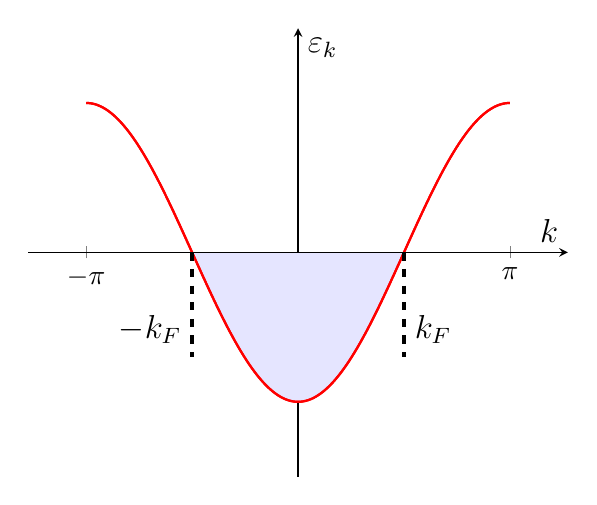
\begin{tikzpicture}
	\begin{axis}[
	legend style={at={(1,0.4)}},
	ytick = {1},
	ytick style={draw=none},
	yticklabels = {},
	xtick = {-3.14159,3.14159},
	xticklabels ={$-\pi$,$\pi$},
	xlabel = \large $k$,
	ylabel = \large $\varepsilon_k$,
	axis lines = center,
	ymin = -1.5,
	ymax = 1.5,
	xmax = 4,
	xmin = -4,
	%x label style={at={(axis description cs:1,0.1)}, anchor = west},
	%y label style={at={(axis description cs:0.15,1)},rotate=-90,anchor=south},
	%xlabel = $x$,
	%sylabel = {$f(x)$},
	]
	
		
		\addplot[name path = A,domain = -1.57:1.57, samples = 200, very thin, black]{(-cos(deg(x)))};
		\addplot[domain = -3.14:3.14, samples = 200, thick, red]{(-cos(deg(x)))};
		\addplot[name path = B, domain = -1.57:1.57] {0*x};
		
		\addplot[blue!10!white] fill between[of = A and B];
		\draw[very thick, black, dashed] (axis cs:-1.57,0) -- node[anchor= north east]{\large $-k_F$}  (axis cs:-1.570,-0.7);
		\draw[very thick, black, dashed] (axis cs:1.57,0) -- node[anchor= north west]{\large $k_F$}  (axis cs:1.570,-0.7);
	\end{axis}
\end{tikzpicture}
	\caption{Dispersion relation. The fermi surface consists of two points}
	\label{fig:disp_rel}
\end{figure}

We are mainly interested in the low energy physics for this problem; We want to describe $\varepsilon_k$ in the vicinity of the Fermi level. In this case, it is especially simple as it only consists of two points, as seen in Figure \ref{fig:disp_rel}.

Right-moving: $k>0$ and left-moving: $k<0$. For both of which we have  $\varepsilon_k\simeq v_F(|k| - k_F)$ and $|k-k_F|<<k_F$. $\varepsilon_k$ is here measured relative the Fermi level.
For every electron spin $\sigma$ we have one type of righ-moving and one type of left-moving fermions, seen in Figure \ref{fig:lr_fermions}.

\begin{figure}
	\centering
	\begin{tikzpicture}
	\begin{axis}[
	legend style={at={(1,0.4)}},
	ytick = {1},
	ytick style={draw=none},
	yticklabels = {},
	xtick = {-3.14159,3.14159},
	xticklabels ={$-\pi$,$\pi$},
	xlabel = \large $k$,
	ylabel = \large $\varepsilon_k$,
	axis lines = center,
	ymin = -1.5,
	ymax = 1.5,
	xmax = 4,
	xmin = -4,
	%x label style={at={(axis description cs:1,0.1)}, anchor = west},
	%y label style={at={(axis description cs:0.15,1)},rotate=-90,anchor=south},
	%xlabel = $x$,
	%sylabel = {$f(x)$},
	]
	
		
		\addplot[name path = A,domain = -3.14:3.14, samples = 200, dashed, black]{(-cos(deg(x)))};
		
		\addplot[domain = -1.77:-1.37, samples = 200,very thick, red]{(-cos(deg(x)))};
		\addplot[domain = 1.37:1.77, samples = 200,very thick, red]{(-cos(deg(x)))};
		
		
		\draw[thick, black, dashed] (axis cs:-1.57,0) -- node[anchor= north east]{\large $-k_F$}  (axis cs:-1.570,-0.5);
		\draw[thick, black, dashed] (axis cs:1.57,0) -- node[anchor= north west]{\large $k_F$}  (axis cs:1.570,-0.5);
	\end{axis}
\end{tikzpicture}
	\caption{The right- and left-moving fermions of interest.}
	\label{fig:lr_fermions}
\end{figure}

\begin{align}
\label{eq:h0_rl}
\begin{split}
\Ha_0 &\simeq \sum_{k,\sigma}v_F(k-k_F)\cd_{1k\sigma}c_{1k\sigma} \\
&+\sum_{k,\sigma}v_F(-k-k_F)\cd_{2k\sigma}c_{2k\sigma},
\end{split}
\end{align}
where $\cd_{1k\sigma}$ creates a right-moving fermion and $\cd_{2k\sigma}$ creates a left-moving fermion etc.
NB: \ref{eq:h0_rl} is defined only at $|\pm k-k_F|<<k_F$!
We write this as
\begin{align}
\begin{split}
\Ha=\sum_{k,\sigma}&\left[\e^{-\alpha|k-k_F|}v_F(k-k_F)\cd_{1k\sigma}c_{1k\sigma}\right. \\
&+\left.\e^{-\alpha|k-k_F|}v_F(-k-k_F)\cd_{2k\sigma}c_{2k\sigma}\right].
\end{split}
\end{align}
Here, $\alpha>0$ is a cutoff-parameter to limit the $k$-summation to those who are close to Fermi level, but in such a way that we can sum over all $k$.
Introduce the real space fermion operators
\begin{align}
\psi_{1\sigma}(x) & =\int\frac{\dd k}{2\pi}c_{1k\sigma}\e^{ikx} \\
\psi_{2\sigma}(x) & =\int\frac{\dd k}{2\pi}c_{1k\sigma}\e^{-ikx},
\end{align}
where the sums over $k$ is calculated close to Fermi-level.
Consider now the free fermion propagators in real space at equal times $(\tau = \tau')$

\begin{align*}
\mathcal{G}_1(x) &= -i\ev{:\psi_{1\sigma}(x)\psi_{1\sigma}^\dagger(x'):}\\
&= -i\int\frac{\dd k}{2\pi}\int\frac{\dd k'}{2\pi}\e^{ik(x-x')}\underbrace{\ev{:c_{1k\sigma}\cd_{1k\sigma}:}}_{=-\delta_{k,k'}n_k} \\
&=i\int_{k<k_F}\frac{\dd k}{2\pi}\e^{-\alpha|k-k_F|}\e^{ik(x-x')} \\
&= i\int_{q<0}\frac{\dd q}{2\pi}\e^{-\alpha|q|}\e^{i(q+k_F)(x-x')} \\
&=i\e^{ik_F(x-x')}\int_{-\infty}^{0}\frac{\dd k}{2\pi}\e^{-\alpha|k| + ik(x-x')}\\
&= i\frac{\e^{ik_F(x-x')}}{2\pi}\int_0^\infty\dd k\,\e^{-k(\alpha + i(x-x'))} \\
&=i\frac{\e^{ik_F(x-x')}}{2\pi}\frac{1}{\alpha + i(x-x')},
\end{align*}
or, to summarize, as $\alpha \rightarrow 0$ (ignoring the short-range cutoff)
\begin{align}
\mathcal{G}_1 &= \frac{1}{2\pi}\frac{\e^{ik_F(x-x')}}{x-x'} \\
\mathcal{G}_2 &= -\frac{1}{2\pi}\frac{\e^{-ik_F(x-x')}}{x-x'}.
\end{align}
Notice the simple poles in the Green's functions. Now, by the $\psi_{1\sigma}$ and $\psi_{2\sigma}$-operators, we have

\begin{equation}
\Ha_0 = v_F\int_{0}^{L}\dd x\left[\psi_{1\sigma}^\dagger\left(-i\partial_x -k_F\right)\psi_{1\sigma} + \psi_{2\sigma}^\dagger\left(i\partial_x - k_F\right)\psi_{2\sigma}\right].
\end{equation}
Defining $\psi_\sigma = \begin{psmallmatrix*} \psi_{1\sigma} & \psi_{2\sigma}
\end{psmallmatrix*}^T$ lets us rewrite this as
\begin{equation}
\label{eq:imp_def_a0}
\Ha_0 = v_F\sum_\sigma\int_{0}^{L}\dd x\,\psi_\sigma^\dagger
\underbrace{\begin{pmatrix}
-i\partial_x - k_F & 0 \\
0 &  i\partial_x - k_F 
\end{pmatrix}}_{A_0}\psi_\sigma
\end{equation}

We now add an interaction term to the theory, on the form
\begin{align*}
\Ha_I &= \sum_{\sigma,\sigma'}\int\dd x\int\dd y\underbrace{\psi_{1\sigma}^\dagger(x)\psi_{1\sigma}(x)}_{\rho_{1\sigma}(x)}v(x-y)\underbrace{\psi_{2\sigma}^\dagger(y)\psi_{2\sigma'}(y)}_{\rho_{2\sigma'}(y)} \\
&= \int \dx\dy \rho_1(x)v(x-y)\rho_2(y).
\end{align*}
We do not consider terms of the types $\rho_1\rho_1, \rho_2\rho_2$; these only contributes to the renormalization of $v_F$. $\rho_1\rho2$ will, however, give rise to more intersting effects.

Therefore, we want to study the theory of

\begin{align}
\begin{split}
\Ha &= v_F \sum_\sigma \int\dx\psi_\sigma^\dagger A_0\psi_\sigma \\
&+ \sum_{\sigma,\sigma'}\int \dx\dy \rho_{1\sigma}(x)v(x-y)\rho_{2\sigma'}(y).
\end{split}
\end{align}

For simplicity, we will in the continuation consider spinless fermions. A spinful treatment will be given later. 

\begin{equation}
\Ha = v_F \int\dx\psi^\dagger A_0\psi+ \int \dx\dy \rho_{1}(x)v(x-y)\rho_{2}(y).
\end{equation}
A spinless system is the same (or equivalent) to a completely spin-polarized problem. We can write down the partition function by applying our normal rules;
\begin{align}
\Z &= \int\D\psi_1^\dagger\D\psi_1\D\psi_2^\dagger\D\psi_2\e^{\Sa} \\
\begin{split}
\Sa &= -\int\dx \int_0^\beta\dd\tau\left(\psi^\dagger\partial_\tau\psi + v_F\psi^\dagger A_0\psi\right) \\
&- \int\dx\int\dy \int_0^\beta\dd\tau\rho_{1}(x)v(x-y)\rho_{2}(y)
\end{split}
\end{align}
Let us simplify the model some more by only considering constant \textit{contact}-interaction between fermions 
\begin{equation}
	v(x-y) = g\delta(x-y); \quad g>0.
\end{equation}

\begin{align*}
	\Sa &= \Sa_0 + \Sa_I \\
	\Sa_0 &= -\int_0^L\dx\int_0^\beta\dd\tau\psi^\dagger\left(\partial_\tau+ v_FA_0\right)\psi \\
	\Z_0 &= \e^{\Tr\ln(\partial_\tau + v_FA_0)} \\
	&= \e^{\int_0^L\dx\int_0^\beta\dd\tau\tr\ln\left(\partial_\tau+ v_FA_0\right)} \\
	\Sa_I &= -g\int\dx\int\dd\tau\rho_1(x)\rho_2(x)
\end{align*}
Now we perform a Hubbard-Stratonovich decoupling og the interaction term in the following way;
\begin{align*}
\int\D\pdag\D\p\,\e^{-(\pdag + g\rho_2)(\p + g\rho_1)g^{-1}} &= \text{const} \\
&= \e^{-\Tr\ln(g^{-1})} = \e^{\ln g} = g.
\end{align*}
Correspondingly,we have
\begin{align*}
\int\D\pdag\D\p\,&\e^{-\int\dx\dd \tau\left(g^{-1}\p^*\p+i\p^*\rho_1 + i\p^*\rho_2\right)} \\
&= \int\D\pdag\D\p\,\e^{-\int\dx\dd \tau\left[g^{-1}(\p^* + ig\rho_2)(\p + ig\rho_1) + g\rho_1\rho_2\right]} \\
&= \e^{-\int\dx\dd \tau g\rho_1\rho_2}\cdot \text{const}.
\end{align*}
The constant is irrelevant and is safely ignored.
\begin{align}
\e^{\Sa_I} &= \int\D\p^*\D\p\e^{-\int\dx\int_0^\beta\left(g^{-1}\p^*\p+i\p^*\rho_1 + i\p\rho_2\right)} \\
\Z &= \int\D\p^*\D\p\D\psi_1^\dagger\D\psi_1\D\psi_2^\dagger\D\psi_2\e^{\Sa[\psi^\dagger,\psi,\p^*\p]}
\end{align}
\begin{equation}
\label{eq:action_1d}
\Sa= -\int_0^L\dx \int_0^\beta \dd\tau \left\{\frac{\p^*\p}{g} +  \psi^\dagger A\psi\right\},
\end{equation}
where\footnote{There is some ambiguity here. In the notes, $\vb{I}$ is denoted $\vec{T}$, so it should be checked that it is the identity operator. We should have a term with $\psi^\dagger\partial_\tau\psi$, so the identity makes sense.}
\begin{equation}
	A \equiv v_FA_0 + \vb{I}\partial_\tau + i
	\begin{pmatrix}
	\p^* & 0 \\
	0 & \p
	\end{pmatrix} = -\mathcal{G}^{-1},
\end{equation}
with $A_0$ defined in \eqref{eq:imp_def_a0}, and
\begin{equation}
	\mathcal{G}(\partial_\tau, x) = -\ev{\psi\psi^\dagger}.
\end{equation}

Note that there is no terms $\sim \p^*\partial_\tau\p$ in \eqref{eq:action_1d}, because the $\p$-field is absent in the Hamiltonian, but is used to decouple the interaction first after the partition function is written down. If we use the spinor-components reduces to 
\begin{equation}
\mathcal{G}(\partial_\tau,x) = -\begin{pmatrix}
\ev{\psi_1\psi_1^\dagger} & 0\\
0 & \ev{\psi_2\psi_2^\dagger}
\end{pmatrix}.
\end{equation}
Since the matrix is diagonal, we can immidiately write down 
\begin{align}\label{eq:greeenss}
\begin{split}
\mathcal{G}_1 &= -(-iv_F\partial_x + \partial_\tau - v_Fk_F + i\p^*)^{-1} \\
\mathcal{G}_2 &= -(iv_F\partial_x + \partial_\tau - v_Fk_F + i\p)^{-1}
\end{split}
\end{align}
The Greens functions \eqref{eq:greeenss} are free Greens functions in \underline{fixed} bosonic background field.
Rewriting these as differential equations, we get
\begin{align}\label{eq:diff_eq_greens}
\begin{split}
(-iv_F\partial_x + \partial_\tau - v_Fk_F + i\p^*)\mathcal{G}_1 &= -\delta(x)\delta(\tau) \\
 (iv_F\partial_x + \partial_\tau - v_Fk_F + i\p)\mathcal{G}_2 &= -\delta(x)\delta(\tau).
\end{split}
\end{align}
NB! These are limited to the one-dimensional case, and are complicated because of the dynamics of $\p(x,\tau), \p^*(x, \tau)$.

\subsection[Free propagators]{Free fermion propagators} % pdf: 245 / notes: 192

The free fermion propagators for our problem is given by

\begin{align}\label{eq:diff_eq_greens}
\begin{split}
(-iv_F\partial_x + \partial_\tau - v_Fk_F )\mathcal{G}_1^0 &= -\delta(x)\delta(\tau) \\
(iv_F\partial_x + \partial_\tau - v_Fk_F)\mathcal{G}_2^0 &= -\delta(x)\delta(\tau).
\end{split}
\end{align}
We want to compute $\mathcal{G}_1,\mathcal{G}_2$ because of all the information these provide to the low-energy physics for the one-dimensional interacting electron gas. Recall the usage as diagnostic tools in the Fermi-liquid case. Now we do a Fourier transform of the equations to obtain
\begin{align}
\nonumber
(iv_Fk+ i\omega_n- v_Fk_F )\mathcal{G}_1^0&= -1 \\
\implies \mathcal{G}_1^0(k,i\omega_n) = \frac{1}{i\omega_n - v_F(k-k_F)} &= \frac{1}{i\omega_n - \varepsilon_1(k)}\\
\nonumber
(-iv_Fk+ i\omega_n- v_Fk_F )\mathcal{G}_2^0&= -1 \\
\implies \mathcal{G}_2^0(k,i\omega_n) = \frac{1}{i\omega_n - v_F(-k-k_F)} &= \frac{1}{i\omega_n - \varepsilon_2(k)},
\end{align}

which are free-form propagators. How does these look like in real space?
Impose, again, a cutoff to make the integral convergent, and set the cutoff-parameter to zero at the end.
\begin{align*}
\mathcal{G}_1^0(x, \tau) &= \int_{-\infty}^\infty\frac{\dd k}{2\pi}\frac{1}{\beta}\sum_{\omega_n}\frac{\e^{ikx - i\omega_n\tau}}{i\omega_n-v_F(k-k_F)}\cdot\underbrace{\e^{-\alpha|k-k_F|}}_{\text{Cutoff-parameter}} \\
&= \int_{-\infty}^\infty\frac{\dd k}{2\pi}\e^{-\alpha|k-k_F| + ikx}f(v_F(k-k_F))\e^{-v_F(k-k_F)\tau}\\
&=\e^{ik-Fx}\int_{-\infty}^0\frac{\dd k}{2\pi}\e^{-\alpha|k| + ikx-v_Fk\tau} \\
&=\frac{\e^{ik_Fx}}{2\pi}\int_0^\infty\dd k\,\e^{-k(\alpha + ix-v_F\tau)} \\
&= \frac{\e^{ik_Fx}}{2\pi}\frac{1}{ix - v_F\tau + \alpha},
\end{align*}
$\alpha = 0^+$. Now let $\tau\rightarrow it$ such that $\mathcal{G}_1^0(x,\tau)\rightarrow i\mathcal{G}_1^0(x, t)$.
\begin{align}
\begin{split}
	\mathcal{G}_1^0(x, t) &=  i\frac{\e^{ik_Fx}}{2\pi}\frac{1}{ix-iv_Ft+\alpha} \\
	&=\frac{\e^{ik_Fx}}{2\pi}\frac{1}{x-v_Ft-i\alpha}
\end{split}
\end{align}
We see that $\mathcal{G}_1^0$ has a pole at $x = v_Ft$. This is classicall linear motion (right-moving). A very similar approach\footnote{The only difference is in the substitution $k' = -k-k_F$ before integrating.} can be used to calculate $\mathcal{G}_2^0$, and leads to 
\begin{equation}
	\mathcal{G}_2^0=\frac{\e^{-ik_Fx}}{2\pi}\frac{1}{-x-v_Ft-i\alpha}, 
\end{equation}
with a pole at $x = -v_Ft$, classical linear motion towards the left.
Therefore, Fermi-liquid propagators also have a simple pole-structure with a simple interpretation in real space. 


\subsection[Interacting propagator]{Propagators in  the interacting case} % pdf:248 / notes 196

The theory is
\begin{align}
\Z &= \int\D\psi^\dagger\D\psi\D\p^*\D\p\e^{\Sa} \\
\Sa &=-\int_0^L\dx\int_0^\tau\dd\tau \frac{\p^*\p}{g}-\int_0^L\dx\int_0^L\dy\int_0^\beta\dd\tau\,\psi^\dagger(x,\tau)A(x,y,\tau)\psi(y, \tau),
\end{align}
\begin{equation*}
A = \begin{pmatrix}
D_1 + i\p^* & 0\\
0 & D_2+i\p
\end{pmatrix}
\end{equation*}

\begin{align*}
D_1 = -&iv_F\partial_x+\partial_\tau-v_Fk_F \\
D_2 =\quad&iv_F\partial_x+\partial_\tau-v_Fk_F
\end{align*}
which is a free fermion system coupled to an external bosonic field $\p$ which fluctuates. Integrating out the fermionic field gives a purely bosonic theory of effective action
\begin{align}
\Z &= \int\D\p^*\D\p\e^{\Sa_{\text{eff}}[\p^*,\p]} \\
\label{eq:s_eff}
\Sa_{\text{eff}} &= \int_{0}^{\beta}\dd\tau\int_{0}^{L}\dx\frac{\p^*\p}{g} + \Tr\ln(D_1+i\p_1) + \Tr\ln(D_2 +i\p_2),
\end{align}
where $\p_1 = \p^*, \p_2 = \p$. 
\begin{align*}
-\mathcal{G}_1^{-1} &= D_1+i\p_1 \\
-\mathcal{G}_2^{-1} &= D_2 +i\p_2
\end{align*}
The propagators above are matrices with $x, \tau;x',\tau'$-indices. $D_i$ includes non local differential operators. We have Green's functions for free fermions coupled to an external bosonic field
\begin{align*}
\mathcal{G}_1 &= \mathcal{G}_1(x, \tau;x', \tau, \p_1) \\\mathcal{G}_2 &= \mathcal{G}_2(x, \tau;x', \tau, \p_2).
\end{align*}

\begin{align}
\label{eq:gre_1}
(D_1+i\p_1)\mathcal{G}_1 &= -\delta(x-x')\delta(\tau-\tau') \\
\label{eq:gre_2}
(D_2 +i\p_2)\mathcal{G}_2 &= -\delta(x-x')\delta(\tau-\tau')
\end{align}

$D_1, D_2$ are 1. order differential operators. Assume now that $x\ne x',\tau\ne\tau'$ such that the right hand side in the equations is zero.
\[D_i\mathcal{G}_i = -i\p_i\mathcal{G}_i \implies \frac{D_i\mathcal{G}_i}{\mathcal{G}_i} = -i\p_i,\quad i = 1,2\]
Now integrate
\begin{align}
\int_{x',\tau'}^{x,\tau}\frac{D_i\gre_i}{\gre_i} &= -i\int_{x',\tau'}^{x,\tau}\p_i \\
\ln\gre_i\bigg{|}_{x',\tau'}^{x,\tau} &= -i\left[f_i(x,\tau,\p_i) - f_i(x',\tau',\p_i)\right]
\end{align}



\[\gre_i = A\e^{-i(f_i(x,\tau)-f_i(x',\tau'))}\]
$\gre_i = \gre_i(x,\tau;x',\tau',\p_i)$. If we now let $\p_i\rightarrow 0 \implies f_i =0$, we must have that $A = \gre_i^0(x-x',\tau-\tau')$. This motivates the following ansatz for the Green's functions in the interacting case:
\begin{equation}
\gre_i(x,\tau;x',\tau',\p_i) = \gre_i^0(x-x',\tau-\tau')\e^{-i\left[f_i(x,\tau,\p_i) - f_i(x',\tau',\p_i)\right]}
\end{equation}

\[D_i\gre_i^0 = -\delta(x-x')\delta(\tau-\tau')\]
The ansatz for $\gre_i$ is now inserted into \cref{eq:gre_1,eq:gre_2}.
$D_i = d_i - V_Fk_F, d_i = \pm iv_F\partial_x + \partial_\tau$.
\begin{align*}
\gre_i(x,\tau;x'\tau') &=(d_i - v_Fk_F+i\p_i)\gre_i^0\e^{-i(f_i-f_i')}\\ &=\left[(d_i-v_Fk_F)\gre_i^0\right]\e^{-i(f_i-f_i')} + i\p_i\gre_i^0\e^{-i(f_i-f_i')} -id_if_i\gre_i^0\e^{-i(f_i-f_i')} \\
&= -\delta(x-x')\delta(\tau-\tau')
\end{align*}
Now use
\begin{align*}
\left[(d_i-v_Fk_F)\gre_i^0\right]\e^{-i(f_i-f_i')} &= -\delta(x-x')\delta(\tau-\tau')\e^{-i(f_i-f_i')}\\&=\delta(x-x')\delta(\tau-\tau');\quad x\ne x',\tau=\tau' \\
\implies  -id_if_i &= -i\p_i
\end{align*}
\begin{align}
-i(-iv_F\partial_x+\partial_\tau)f_1 &= -i\p_1 \\
-i(iv_F\partial_x+\partial_\tau)f_2 &= -i\p_2
\end{align}
To continue, we fourier transform these equations. Since $\p_i$ are bosonic fields, $f_i$ are aswell, and Fourier-transform with bosonic matsubara frequencies \[\omega_\nu = \frac{2\pi\nu}{\beta}\quad;\nu = 0,\pm1,\dots\].
\begin{align}
f_i(x,\tau) &= \frac{1}{\beta}\int\frac{\dd k}{2\pi}\sum_{\omega_\nu}f_i(k,\omega_\nu)\e^{i(kx-\omega_\nu\tau)}\\
\label{eq:fourier_transformed_1d_fields}
\p_i(x,\tau) &= \frac{1}{\beta}\int\frac{\dd k}{2\pi}\sum_{\omega_\nu}\p_i(k,\omega_\nu)\e^{i(kx-\omega_\nu\tau)}
\end{align}
Inserting these gives
\begin{align}
\nonumber
-i(v_Fk-i\omega_\nu)f_i(k,i\omega_\nu) &= -i\p_i(k,i\omega_\nu) \\
\implies f_1(k,i\omega_\nu) 
&= -\frac{\p_1(k,i\omega_\nu)}{i\omega_\nu - v_Fk}, \\
f_2(k,i\omega_\nu) &= -\frac{\p_2(k,i\omega_\nu)}{i\omega_\nu + v_Fk}
\end{align}

Transforming back to real space, using
\begin{equation}
\label{eq:fourier_transformed_field_2}
f_i(x,\tau) = -\frac{1}{\beta}\int\frac{\dd k}{2\pi}\sum_{\omega_\nu}\frac{\p_i(k,i\omega_\nu)}{i\omega_\nu \mp v_Fk}\e^{i(kx-\omega_\nu\tau)}
\end{equation}
with upper ($i=1$) and lower($i=2$). We have now in principle found
\begin{equation}
	\gre_i(x,\tau;x',\tau',\p_i) = \gre_i^0(x-x',\tau-\tau')\e^{-i\left[f_i(x,\tau,\p_i)-f_i(x',\tau',\p_i)\right]},
\end{equation}
which was the ansatz. But this is \underline{not} the physical electron-propagators for the system! 
The propagator \(\gre_i\) seperates from the free propagators only by a phase factor, and must be understood as free fermion propagators in a given bosonic background field where the field configuration for the bosons are specified.
The physical fermion propagator is found by averaging $\gre_i$ over the fields $\p_i$. 
We thus want to compute
\begin{equation}
\label{eq:averaged_greens}
\ev{\gre_i}_{\p_i} = \frac{\int\D\p^*\D\p\gre_i(x, \tau;x', \tau', \p_i)\e^{\Sa_{\text{eff}}}}{\int\D\p^*\D\p\e^{\Sa_{\text{eff}}}}.
\end{equation}
To get any further with this problem, we must have an explicit expression for $\Sa_{\text{eff}}$ in terms of $\p^*,\p$. We will look more into this, but the followin discussion will be general to begin with. We had \cref{eq:s_eff}
\begin{equation*}
\Sa_{\text{eff}} = \int_{0}^{\beta}\dd\tau\int_{0}^{L}\dx\frac{\p^*\p}{g} + \Tr\ln(D_1+i\p_1) + \Tr\ln(D_2 +i\p_2),
\end{equation*}
which, for a free system is
\begin{equation}
\Sa_0 =\sum_{i=1}^2\Tr\ln(D_i).
\end{equation}
This contribution is of no importance when averaging over $\p_i$-configurations, and we therefore substract it.
Remember:
\begin{align*}
	(D_i + i\p_i) &= -\gre_i^{-1}(x,\tau;x',\tau',\p_i) \\
	(D_i + i\p_i)&^{-1} = -\gre_i(x,\tau;x',\tau',\p_i)
\end{align*}

\begin{align*}
\ln(D_i + i\p_i) &= \ln D_i + \ln\left(\frac{D_i+i\p_i}{D_i}\right) \\
&=\ln D_i +i\p_i\int_0^1\dd\lambda\left(D_i+\i\p_i\lambda\right)^{-1} \\
&=\ln D_i - i\p_i\int_0^1\dd\lambda\underbrace{\gre_i(x,\tau;x'\tau',\lambda\p_i)}_{\text{matrix}}
\end{align*}
$\Tr\ln(D_i+i\p_i)$ means suming over the diagonal elements of $\ln(D_i+i\p_i)$. The first term gives a free-electron contribution, and is known. 
We now have to calculate the sum of the diagonal-elements in the matrix
\begin{equation}
	\p_i(x,\tau)\int_{0}^{1}\dd\lambda\gre_i(x,\tau;x'\tau',\lambda\p_i),
\end{equation}
which involves letting $x\rightarrow x', \tau\rightarrow\tau'$ in $\gre_i$ and thereafter integrate over $\lambda$.
Since $\gre_i^0(x-x',\tau-\tau')$ is divergent in this limit, we must be careful when considering this limit. First look at $\gre_1$:
\begin{equation}
\gre_1 = \gre_1^0\e^{-i\left[f_1(x,\tau)-f_1(x',\tau')\right]}.
\end{equation}
Set $\tau =\tau'$. Now we can evaluate the limit $x\rightarrow x'$ in two ways; $x'$ can approach $x$ either from above or below \[x'\rightarrow x\pm\eta;\quad \eta = 0^+\]
We treat the transition as an average of both ways.
\begin{align}
\gre_1^0 &= \frac{1}{2\pi}\frac{\e^{ik_F(x-x')}}{i(x-x') \mp ik_F\eta} \\
&\implies \frac{1}{2\pi}\frac{\e^{\mp ik_F\eta}}{i\mp\eta}\rightarrow \mp\frac{1}{2\pi\eta i}
\end{align}
%\subsection{The phase factor} % 258 / 203
Consider now the phase factor of $\gre_1$;


\begin{align*}
f_1(x,\tau) - f_1(x\pm\eta,\tau) &= f_1(x,\tau) - f_1(x,\tau) \mp\eta\pdv{f_1}{x} \\
&= \mp\eta\pdv{f_1}{x} \\
\lim\limits_{x\rightarrow x'}\gre_1(x,\tau;x',\tau,\lambda\p_1) &= \frac{1}{2}\left(\frac{-1}{2\pi i}\right)\left[\frac{1}{\eta}\e^{i\eta\pdv{f}{x}} - \frac{1}{\eta}\e^{-i\eta\pdv{f}{x}}\right] \\
&= \frac{-1}{4\pi i\eta}\left[1+i\eta\pdv{f_1}{x} - \left(1-i\eta\pdv{f_1}{x}\right)\right] \\
&= -\frac{1}{2\pi}\pdv{f_1(x,\tau,\lambda\p_1)}{x} \\
\lim\limits_{x\rightarrow x'}\gre_2(x,\tau;x',\tau,\lambda\p_2) &= \frac{1}{2\pi}\pdv{f_1(x,\tau,\lambda\p_2)}{x}
\end{align*}
\begin{align*}
\Sa_{\text{eff}} = \Sa_0 &- \int_0^L\dx\int_0^\beta\dd\tau\frac{\p_1\p_2}{g}\\&-i\int_0^1\dd\lambda\int_0^L\dx\int_0^\beta\dd\tau\left[\p_1\left(\frac{-1}{2\pi}\pdv{f_1(\lambda\p_1)}{x}\right) + \p_2\frac{1}{2\pi}\pdv{f_2(\lambda\p_2)}{x}\right] \\
=\Sa_0 &- \int_0^L\dx\int_0^\beta\dd\tau\frac{\p_1\p_2}{g}\\
&+\frac{i}{2\pi}\underbrace{\int_0^1\dd\lambda\,\lambda}_{\flatfrac{1}2}\int_0^L\dx\int_0^\beta\left[\p_1\pdv{f_1(\p_1)}{x} -\p_2\pdv{f_2(\p_2)}{x}\right],
\end{align*}
where we used that \(f_i(x, \tau, \lambda\p_io) = \lambda f_i(x, \tau, \p_i)\) to extract and integrate out $\lambda$.
But \(f_i\sim\p_i\) implies that \( \Sa_{\text{eff}}(\p^*,\p)\) is quadratic in the $\p$-fields. Thus, we have an exact effective action as a free boson theory!
It is worth noticing how this remarkable result was achieved; It originates from the form \[\gre_i=\gre_i^0\e^{-i(f_i-f_i')}\]
Naturally, we can write an ansatz like this for the Green's function for an arbitrary, if only the $f_i$-fields are properly chosen. In our case, where the spectrum is \textit{linearized}, the differential equation for $f_i$ is especially simple, such that $f_i \sim\p_i$. Because of this, $\Sa_{\text{eff}}$ becomes quadratic in $\p_i$. More generally, $f_i$ would become complicated functions of $\p_i$, and the resulting boson-theory would be complicated and interacting. 

\label{sect:1}
In the following we will exclude \(\Sa_{0}\) from \(\Sa_{\text{eff}}\) as it does not contribute to the averaging over the $\p_i$-fields. The effective action is
\begin{equation}
\label{eq:1d_effective_action}
\Sa_{\text{eff}} = -\int_0^L\dx\int_0^\beta\dd{\tau}\left[\frac{\p_1\p_2}{g} - \frac{i}{4\pi}\left(\p_1\pdv{f_1}{x}-\p_2\pdv{f_2}{x}\right)\right].
\end{equation}

Recall the fourier transformed fields in \cref{eq:fourier_transformed_1d_fields,eq:fourier_transformed_field_2}, and insert them  in the first term of \cref{eq:1d_effective_action}. We then get
\begin{align*}
-\int\dx\int\dd\tau\frac{\p_1\p_2}{g} &= -\frac{1}{g}\int\dx\int\dd{\tau}\frac{1}{\beta}\sum_{\omega_{\nu_1}}\int\frac{\dd{k_1}}{2\pi}\frac{1}{\beta}\sum_{\omega_{\nu_2}}\int\frac{\dd{k_2}}{2\pi} \\
&\quad\times \e^{i(k_1+k_2)x - i(\omega_{\nu_1}+\omega_{\nu_2}\tau)}\p_1(k_1,\omega_{\nu_1})\p_2(k_2, \omega_{\nu_2})\\
&= -\frac{1}{\beta g}\sum_{\omega_\nu}\int\frac{\dd{k}}{2\pi}\p_1(k,\omega_\nu)\p_2(-k,-\omega_\nu),
\end{align*}
where the integration over $x, \tau$ has given $\delta$-functions in $k,\omega_\nu$.
Now take the second term, the term with $p_1$, insert the Fourier transformed forms, and get
\begin{align*}
\frac{i}{4\pi}\int\dx\int\dd{\tau}\p_1\pdv{f_1}{x} &= \frac{i}{4\pi}\int\dx\int\dd{\tau}\frac{1}{\beta}\sum_{\omega_{\nu_1}}\int\frac{\dd{k_1}}{2\pi}\p_1(k_1, \omega_{\nu_1})\e^{i(k_1x - \omega_{\nu_1}\tau)} \\&\quad\times \pdv{x}\frac{-1}{\beta} \sum_{\omega_{\nu_2}}\int\frac{\dd{k_2}}{2\pi}\frac{\p_1(k_2, \omega_{\nu_2})}{i\omega_{\nu_2} - v_Fk_2}\e^{i(k_2x - \omega_{\nu_2}\tau)} \\
&= \frac{i}{4\pi}\int\dx\int\dd{\tau}\frac{1}{\beta}\sum_{\omega_{\nu_1}}\int\frac{\dd{k_1}}{2\pi}\p_1(k_1, \omega_{\nu_1})\e^{i(k_1x - \omega_{\nu_1}\tau)} \\&\quad\times \frac{-1}{\beta} \sum_{\omega_{\nu_2}}\int\frac{\dd{k_2}}{2\pi}\frac{ik_2\p_1(k_2, \omega_{\nu_2})}{i\omega_{\nu_2} - v_Fk_2}\e^{i(k_2x - \omega_{\nu_2}\tau)} \\
&= -\frac{i^2}{4\pi}\int\frac{\dd{k}}{2\pi}\frac{1}{\beta}\sum_{\omega_\nu}\frac{k}{i\omega_\nu-v_Fk}\p_1(k, \omega_\nu)\p_1(-k,-\omega_\nu) \\
&= -\frac{1}{\beta}\int\frac{\dd{k}}{2\pi}\sum_{\omega_\nu}A_1(k,\omega_\nu)\p_1(k, \omega_\nu)\p_1(-k,-\omega_\nu), 
\end{align*}
where \[A_1(k,\omega_\nu) = -\frac{1}{4\pi}\frac{k}{i\omega_\nu - v_Fk}.\]
Similarly for the $\p_2$-term;
\[A_2(k,\omega_\nu) = \frac{1}{4\pi}\frac{k}{i\omega_\nu +v_Fk}.\]
Combining it all, we have
\begin{align}
\begin{split}
\Sa_{\text{eff}} &= -\frac{1}{\beta}\sum_{\omega_\nu}\int\frac{\dd{k}}{2\pi}\left[\frac{\p_1(k,\omega_\nu)\p_2(-k,-\omega_\nu)}{g}\right. \\
&\quad+ A_1\p_1(k,\omega_\nu)\p_1(-k,-\omega_\nu)
+ A_2\p_2(k,\omega_\nu)\p_2(-k,-\omega_\nu)\left.\vphantom{\int}\right],
\end{split}
\end{align}
effective action in quadratic form!
We are now come so far that we can compute \(\ev{\gre_i(x, \tau;x', \tau', \p_i)}_{\p_i}\)
Inserting what we know in \cref{eq:averaged_greens}, with \[\gre_1^0 = \frac{1}{2\pi}\frac{\e^{ik_F(x-x')}}{i(x-x')-v_F(\tau-\tau') + \alpha} ; \quad \alpha = 0^+.\]
$\gre_1^0$ goes outside as a multiplicative factor, since it does not depend on the bosonic fields. 
\begin{align*}
-i\left[f_1(x, \tau, \p_1) - f_1(x', \tau', \p_1)\right] &= -i\frac{-1}{\beta}\int\frac{\dd{k}}{2\pi}\sum_{\omega_\nu}\frac{1}{i\omega_\nu-v_Fk}\p_1(k, \omega_\nu) \\
&\quad\cdot\left[\e^{i(kx-\omega_\nu\tau)} - \e^{i(kx'-\omega_\nu\tau')}\right] \\
&=\frac{-i}{\beta}\sum_{\omega_\nu}\int\frac{\dd{k}}{2\pi}\p_1(k, \omega_\nu)\J_1(k, \omega_\nu, x, \tau;x', \tau'),\\
\J_1&\equiv \frac{-1}{i\omega_\nu-v_Fk} \left[\e^{i(kx-\omega_\nu\tau)} - \e^{i(kx'-\omega_\nu\tau')}\right]
\end{align*}
Now define 
\begin{equation}
\Z_\p = \int\D\p_1\D\p_2\e^{\Sa_{\text{eff}}}.
\end{equation}
The average can be written as
\begin{align*}
\ev{\gre_1}_\p = \frac{\gre_1^0}{\Z_\p} \int \D\p_2\D\p_2 &\exp \left\{ -\frac{1}{\beta}\sum_{\omega_\nu}\int\frac{\dd{k}}{2\pi} \left[\frac{\p_1\p_2}{g}\right.\right.\\
& \left.\left.+A_1\p_1\p_1+ A_2\p_2\p_2+ \frac{i}{2}\left(\p_1\J_1 + \p_2\J_2\right)\right]\vphantom{-\frac{1}{\beta}\sum_{\omega_\nu}\int\frac{\dd{k}}{2\pi} \left[\frac{\p_1\p_2}{g}\right. }\right\}.
\end{align*}
\underline{The exponent:}

\begin{align*}
\p_1(k)\frac{1}{g}\p_2(-k) &+ A_1\p_1(k)\p_1(-k) \\
&\quad + A_2\p_2(k)\p_2(-k) + \frac i2\left(\p_1(k)\J_1(k) + \underbrace{\p_1^*(-k)}_{\sim\p_2(-k)}\J_1^*\right) \\
&= \left(\p_1+\frac{i}{2}D\J_1^*\right)D^{-1}\left(\p_2+\frac{i}{2}D\J_1\right) + \frac{D}{4}|\J_1|^2. 
\end{align*}
This allows us to write
\begin{equation}
\label{eq:gre_almost_final}
\ev{\gre_1}_\p = \gre_1^0\frac{1}{\Z_\p}\Z_\p\e^{-Q(x, \tau;x',\tau')}
\end{equation}
with
\begin{equation}
\label{eq:Q}
Q = \frac{1}{4\beta}\sum_{\omega_\nu}\int\frac{\dd{k}}{2\pi}D|\J_1|^1, .
\end{equation}
and
\begin{align*}
|\J_1|^2 &= 2\left[1-\cos(k(x-x')-\omega_\nu(\tau-\tau'))\right]\frac{1}{\omega_\nu^2 + k^2v_F^2}\\
D^{-1} &= \frac{1}{g} + A_1+A_2 \\
&= \frac1g-\frac{k}{4\pi}\left(\frac{1}{i\omega_\nu - v_Fk}-\frac{1}{i\omega_\nu+v_Fk}\right) \\
&=\frac{1}{g}-\frac{k}{4\pi}\frac{2v_Fk}{(i\omega_\nu)^2-(v_Fk)^2} \\
&=\frac{1}{g}\frac{(i\omega_\nu)^2-(v_Fk)^2-(v_Fk)^22\tilde{g}}{(i\omega_\nu)^2-(v_Fk)^2} \\
&= \frac1g \frac{(i\omega_\nu)^2-(v_Fk)^2(1+2\tilde{g}}{(i\omega_\nu)^2-(v_Fk)^2},
\end{align*}
where we defined \(\tilde{g} = \frac{g}{4\pi v_F}\). Multiplying \(D\) with \(|\J|^2\), we obtain
\begin{equation}
D|\J_1|^2 = \frac{2g\left(1-\cos\left[k(x-x')-\omega_\nu(\tau-\tau')\right]\right)}{\omega_\nu^2+(v_Fk)^2(1+2\tilde{g})}.
\end{equation}
Inserting this into \cref{eq:Q}, we get
\begin{equation}
\label{eq:Q_1}
Q(x, \tau) = \frac{g}{2\beta}\sum_{\omega_\nu}\int\frac{\dd{k}}{2\pi}\frac{\left[1-\cos\left(kx-\omega_\nu\tau\right)\right]}{\omega_\nu^2+(v_Fk)^2(1+2\tilde{g})}
\end{equation}
Set \(\tau = 0\) and do the frequency summation
\begin{equation*}
	\frac1\beta\sum_{\omega_\nu}\frac{1}{\omega_\nu^2 +\varepsilon_k^2} = -\frac{1}{2\varepsilon_k}\left(\frac{1}{\e^{-\beta\varepsilon_k}-1} - \frac{1}{\e^{\beta\varepsilon_k}-1}\right)
\end{equation*}
At $T = 0$, the first term only contributes if $k>0$ and the second only if $k<0$. 
\begin{align*}
	Q(x) &= -\frac{g}{2}\frac{1}{2\pi v_F\sqrt{1+2\tilde{g}}}\left[\int_{-\infty}^{0}\dd{k}\frac{1-\cos(kx)}{k}-\int_0^\infty\dd k\frac{1-\cos(kx)}{k}\right] \\
	&=\underbrace{\frac{g}{2}\frac{2}{2\pi v_F\sqrt{1+2\tilde{g}}}}_{\equiv 2\nu}\underbrace{\int_0^\infty\dd k\left(\frac{1-\cos(kx)}{k}\right)\e^{-\Lambda k}}_{\equiv H(x)}.
\end{align*}
Thus we have, with \(\nu = \frac{\tilde{g}}{\sqrt{1+2\tilde{g}}}\),
\begin{equation}
Q(x) = 2\nu H(x)
\end{equation}
The factor \(e^{-\Lambda x}\) is introduced as a cutoff on the momentum transfer in a forward-scattering process. This \(\Lambda\)-factor is \underline{not} related to the facto \(\e^{-\alpha|k|}\) which we used as a cutoff on the spectrum for the free fermions. NB: Notice how completely wrong a mean field theory of the bosonic sector would be, in this case!
\begin{align*}
\pdv{H}{x} &= \int_0^\infty\dd k \e^{-\Lambda k}\sin(kx) \\
&= \frac{x}{x^2+\Lambda^2} \\
\implies H &= \frac12\ln\left(\frac{x^2+\Lambda^2}{\Lambda^2}\right) \\
\implies Q(x) &= 2\nu\frac12\ln\left(\frac{x^2+\Lambda^2}{\Lambda^2}\right) \\
&= \ln\left[\left(\frac{x^2+\Lambda^2}{\Lambda^2}\right)^\nu\right] 
\end{align*}
We can now write down the Green's function by inserting the results in \cref{eq:gre_almost_final} and obtain
\begin{equation}
\ev{\gre_1}_\p = -\ev{\psi_1\psi_1^\dagger} = \frac{1}{2\pi}\frac{\e^{ik_F(x-x')}}{i(x-x')+\alpha}\cdot\left(\frac{\Lambda^2}{(x-x')^2+\Lambda^2}\right)^\nu
\end{equation}
Notice how the propagator returns to a free fermion propagator if the interaction is zero (\(g\rightarrow0\)). 
The propagator has now gained a singularity that is not only simple poles. No longer a Fermi-fluid!
The factor \(\left(\frac{\Lambda^2}{x^2+\Lambda^2}\right)\) describes a ``cloud'' of particle-hole excitations that the electron ``carries'' along.


\subsection{The bosonic excitation spectrum} % 270 / 212a


The action
\begin{equation}
	\Sa_{\text{eff}} = -\frac1\beta\sum_{\omega_\nu}\int\frac{\dd k}{2\pi}\left(\frac1g\p_1\p_2+A_1\p_1\p_1^*+A_2\p_2\p_2^*\right)
\end{equation}
ucan be rewritten, by introducing \(\p = \begin{psmallmatrix}
\p_1 \\ \p_2 
\end{psmallmatrix}\), as
\begin{equation}
\Sa_{\text{eff}} = -\frac1\beta\sum_{\omega_\nu}\int\frac{\dd k}{2\pi}\p^*\begin{pmatrix}
A_1 & \frac{1}{2g} \\
\frac{1}{2g} & A_2
\end{pmatrix}\p.
\end{equation}
The free energy is
\begin{equation}
-\beta F = -\frac1\beta\sum_{\omega_\nu}\int\frac{\dd k}{2\pi}\left(\ln(A_1A_2-\frac{1}{4g^2})\right) - \beta F_0,
\end{equation}
where \(F_0\) is the free energy for noninteracting cases (remember ignoring  \(\Sa_0\) in the calculations from \cref{eq:1d_effective_action} and onwards).
\begin{align*}
A_1A_2 -\frac{1}{4g^2} &= -\left(\frac{k}{4\pi}\right)^2\frac{1}{(i\omega_\nu)^2-v_F^2k^2} - \frac{1}{4g^2} \\
&= -\frac{1}{4g^2}\left(1+\frac{4g^2\left(\frac{k^2}{4\pi}\right)^2}{(i\omega_\nu)^2-v_F^2k^2}\right) \\
&=-\frac{1}{4g^2}\frac{\left[(i\omega_\nu)^2 - v_F^2k^2(1-(2\tilde{g})^2)\right]}{(i\omega_\nu)^2-v_F^2k^2},
\end{align*}
where \(\tilde{g} = \flatfrac{g}(4\pi v_F)\) as earlier. Introducing \(u^2 \equiv v_F^2(1-(2\tilde{g})^2)\), and dropping \(\ln(\frac{1}{4g^2})\) from the free energy (as it is an irrelevant constant), we can write
\begin{equation}
-\beta F = -\beta F_0 -\frac{1}{\beta}\sum_{\omega_\nu}\int\frac{\dd k}{2\pi}\left\{\left[\ln((i\omega_\nu)^2-u^2k^2)\right] - \left[\ln((i\omega_\nu)^2-v_F^2k^2)\right]\right\}.
\end{equation}
We will now see that the free energy for the non-interacting case cancels $F_0$! Doing the summation over the bosonic matsubara frequencies, as we have done before, we have
\begin{align*}
-\beta F = \int\frac{\dd k}{2\pi}\ln\left(\frac{-1}{4g^2}\right) &+ \underbrace{\int\frac{\dd k}{2\pi} \left[\ln\left(\overbrace{1+\e^{-\beta v_Fk}}^{\text{Right-moving}}\right)+ \ln\left(\overbrace{1+\e^{\beta v_Fk}}^{\text{Left-moving}}\right)\right]}_{\text{Free fermion-part}}\\
&+ \int\frac{\dd k}{2\pi}\left[\ln\left(1-\e^{-\beta uk}\right) + \ln\left(1-\e^{\beta uk}\right)\right] \\
&+ \underbrace{\int\frac{\dd k}{2\pi}\left[\ln\left(1-\e^{-\beta v_Fk}\right) + \ln\left(1-\e^{\beta v_Fk}\right)\right]}_{\text{Free boson part}}
\end{align*}
Now consider the $T\rightarrow 0$ limit, since the issue of Fermi-liquid vs non-Fermi-liquid \underline{is} a $T =0$-issue.
\begin{align*}
-\beta F &= \int_{-\infty}^0\frac{\dd k}{2\pi}\ln\left(\frac{-1}{4g^2}\right)  \\
&+ \int_{-\infty}^0\frac{\dd k}{2\pi}\left(-\beta v_Fk\right) &+ \int_{0}^\infty\frac{\dd k}{2\pi}\beta v_Fk \\
&+ \int_{-\infty}^0\frac{\dd k}{2\pi}\left[\ln(-1) -\beta uk\right]
&+\int_{0}^\infty\frac{\dd k}{2\pi}\left[\ln(-1) +\beta uk\right] \\
&-\int_{-\infty}^0\frac{\dd k}{2\pi}\left[\ln(-1) + (-\beta v_Fk)\right]
&-\int_0^\infty \frac{\dd k}{2\pi}\left[\ln(-1) + \beta v_Fk\right] \\
&= const -\beta\int_{-\infty}^\infty\frac{\dd k}{2\pi}uk 
\end{align*}
\(E_0 = \sum_k u\cdot k\), so we have a Boson system with excitation spectrum \(\omega = uk\), with 
\begin{equation}
u =v_F\left(1-(2\tilde{g})^2\right)^{\frac12}.
\end{equation}
The ``speed of sound'' for the bosons are thus renormalized in comparison to the fermi-velocities \(v_F\) for the non-interacting fermions. These bosons are collective excitations built from fermions, and is anolgous to phonons (``sound waves'' in a lattice).

Now look at the Greens function for \(\tau \ne\tau'\)\footnote{So far we have considered \(\tau=0\).}. Going back to \eqref{eq:Q_1}, 
\begin{align*}
Q(x, \tau) &= \frac{g}{2\beta}\sum_{\omega_\nu}\int_{-\infty}^\infty\frac{\dd{k}}{2\pi}\frac{\left[1-\cos\left(kx-\omega_\nu\tau\right)\right]}{\omega_\nu^2+u^2k^2} \\
&= -\frac{g}{2\beta}\sum_{\omega_\nu}\int_{-\infty}^\infty\frac{1}{2uk}\frac{\dd{k}}{2\pi}\left[1-\cos\left(kx-\omega_\nu\tau\right)\right]% \\ &\quad 
\cdot \left(\frac{1}{i\omega_\nu -uk} - \frac{1}{i\omega_\nu+uk}\right) \\
&= -\frac{g}{4\pi u}\int_{-\infty}^\infty\dd k\frac{\e^{-\Lambda |k|}}{k}\left\{-n_B(uk)\left[1-\cos\left(kx+iuk\tau\right)\right] +n_B(-uk)\left[1-\cos\left(kx-iuk\tau\right)\right] \right\},
\end{align*}
where the function $n_B$ is (at $T=0$), in terms of Heaviside step-functions as
\begin{align}
\begin{split}
n_B(uk) = -\theta(-k)\\
n_B(-uk) = -\theta(k),
\end{split}
\end{align}
and \(u^2=v_F^2(1+2\tilde{g})\).
Introducing \(x_\pm\equiv x\pm ik\tau\), and recognizing the quantity \(\flatfrac{g}(4\pi u)\) as\footnote{In the lecture notes, it is some uncertainty regarding the definition of \(\nu\), but this seems to do the trick.}
\begin{equation*}
\frac{g}{4\pi u} = \frac{g}{4\pi v_F(1-(2\tilde{g})^2)^{\frac{1}{2}}} =\frac{\tilde{g}}{\sqrt{1+2\tilde{g}}}  = \nu,
\end{equation*}
we can calculate \(Q\) to be
\begin{align*}
	Q(x, \tau) &=\frac{g}{4\pi u}\left\{\int_0^\infty\dd {k}\frac{\e^{-\Lambda k}}{k}\left[1-\cos(kx_+)\right] \right. \\
	&\qquad\quad + \left.\int_0^\infty \dd{k}\frac{\e^{-\Lambda k}}{k}\left[1-\cos(kx_-)\right]
	\right\} \\
	&= 2\nu\frac12\frac12\ln\left(\left(\frac{x_+^2+\Lambda^2}{\Lambda^2}\right)\left(\frac{x_-^2+\Lambda^2}{\Lambda^2}\right)\right) \\
	&=\ln\left(\frac{\left[(x_+^2+\Lambda^2)(x_-^2+\Lambda^2)\right]^{\frac12}}{\Lambda^2}\right)^\nu.
\end{align*}
The explicit form of the total Greens' function then becomes, by inserting into the definition of \cref{eq:gre_almost_final}, as

\begin{equation}
\gre_1(x, \tau) = \gre_1^0(x, \tau)\cdot\left(\frac{\Lambda^2}{\left[(x_+^2+\Lambda^2)(x_-^2+\Lambda^2)\right]^{\frac12}}\right)^\nu
\end{equation}
Notice how completely wrong a mean-field theory for the bosonic action would have been in this case.

\subsection{Impulse distribution} % 277 / 212f  Kanskje ta side 212a - 212g i samme subsection?
We will now briefly study the distribution in momentum-space, by considering
\begin{equation*}
n_k = \mathcal{F}[\psi^\dagger(x)\psi(x)] = 1-\mathcal{F}[\gre(x)].
\end{equation*}
\[\gre(x) = \frac{\e^{ik_Fx}}{2\pi}\frac{i}{x-i\alpha}\left(\frac{\Lambda^2}{x^2+\Lambda^2}\right)^{2\nu}\]

\begin{align*}
\int_{-\infty}^\infty\dx\e^{-ikx}\gre(x) &= \frac{1}{2\pi}\int_{-\infty}^\infty\dx\frac{i}{x-i\alpha}\left(\frac{\Lambda^2}{x^2+\Lambda^2}\right)^{2\nu}\e^{-i(k-k_F)x} \\
&= \frac{1}{\pi}\int_0^\infty\dx\frac{1}{x}\left(\frac{\Lambda^2}{x^2+\Lambda^2}\right)^{2\nu}\sin((k-k_F)x)\\
&= \frac{\sign(k-k_F)}{\pi}\underbrace{\int_0^\infty\dx\frac1x\left(\frac{1}{1+x^2}\right)^{2\nu}\sin(|k-k_F|\Lambda x)}_{(\Lambda|k-k_F|)a_1 + (\Lambda|k-k_F|)^{4\nu}a_2},
\end{align*}
where \(a_1 = a_1(\nu, \Lambda|k-k_F|)\) and correspondingly for \(a_2\) are smooth functions. \footnote{This section should perhaps be expanded upon. There is a reference in the notes, but it is not easy to find; ``G.R. 3.773.1''}
\begin{equation}
n_k = 1-\sign(k-k_F)(\Lambda|k-k_F|)^{4\nu}
\end{equation}
\begin{figure}
	\centering
	\begin{tikzpicture}%[scale = 0.75]
\begin{axis}[
	%ticks = none,
	ytick = {1},
	yticklabels = {,,},
	xtick = {0},
	xticklabels = {$k_F$},
	xlabel = $k$,
	ylabel = $n_k$,
	x label style={at={(axis description cs:1,0.1)}, anchor = west},
	y label style={at={(axis description cs:0.15,1)},rotate=-90,anchor=south},
	ymax = 2,	
	axis lines = left]


\draw[thick,dashed, red] (axis cs:-5,1) --  (axis cs:0,1);
\draw[thick,dashed, red] (axis cs:0,1) --  (axis cs:0,0);

\addplot[thick,samples=100,black, domain =-5:5] {(1/((exp((2*x)))+1))};
%\addplot[thick,samples=100,black, domain =0:5] {(1/((exp((x)))+1)) - 0.4};
%\draw[very thick, black] (axis cs:0,0.5) -- node[anchor= west]{\large $z_k$}  (axis cs:0,0.1);



\end{axis}
\end{tikzpicture}
	\caption{The impulse distribution, or occupation number in momentum-space}
	\label{fig:occupation_k}
\end{figure}
Illustrating this result in \cref{fig:occupation_k}, we see that the discontinuity at Fermi-level is gone! Also from this it is clear that we are not dealing with a Fermi-fluid.

\subsection[Summary]{Summary of spinless 1d interacting systems} % 279 / 213

In one-dimensional systems we do \underline{not}, unlike the three-dimensional, that mean field theories will work. 
\begin{itemize}
	\item \textbf{D=3}: We expect that both thermal fluctuations and quantum fluctuations are unimportant, except near critical temperatures.
	\item \textbf{D=2}: Quantum fluctuations are unimportant. Thermal fluctuations are always important, $T>0$ for systems with a continous symmetry (Mermin-Wagner theorem).
	\item \textbf{D=1}: Both thermal and quantum fluctuations are always important.
\end{itemize}
Fluctuations gets increasingly important when lowering the spatial dimension. In our one-dimensional case we have seen how important these fluctuations can be; if we would have used a mean field approach for calculating the effective action $\Sa_{\text{eff}}$, we would have found Fermi-liquid Green's functions for the electrons! \textbf{It is the boson-fluctuations that are responsible for the destruction of the Fermi liquids in this case!}
The more conventional view in one dimension, is that forward scattering is \underline{singular} (because the electrons cannot avoid each other), and that this destroys the one-particle picture.

These viewpoints can be united in the following manner:
In mean field theory, the fermions are renormalized, free, and noninteracting electrons. The bosonic fields was introduced in the H-S-decoupling of the interaction term in the Hamiltonian. The boson fluctuations thus represent the residual interaction between electrons, and this interaction is in our case of forward scattering type. When these fluctuations are integrated out, the resulting fermion propagators are qualitatively different from before. We end up with propagators that do not any longer contain simple poles as singularities. The quasiparticle picture is destroyed by the string fluctuations originating in forward scattering.
We have seen that the effective action is a free boson theory. The system \underline{does} have well defined one-particle boson-excitations, but it does not have fermionic quasiparticles! An interacting fermion system is exactly replaced by a free boson system. 
\textbf{A system of interacting fermions with gapless bosonic excitations as its low-energy excitations, is called a Luttinger liquid.}
The low-energy excitations (the $\p$'s) for such a system is called Tomonaga-Luttinger bosons. If we had included spin in the system, and considered forward scattering, we would have obtained \(\Sa_{\text{eff}} = \Sa_{\text{eff}}^\rho + \Sa_{\text{eff}}^\sigma\), where \(\Sa_{\text{eff}}^\rho\) describes the Tomonaga-uttinger bosons with charge, but no spin, and \(\Sa_{\text{eff}}^\sigma\) describes Tomonaga-Luttinger bosons with spin, but no charge. There is no coupling between \(\Sa_{\text{eff}}^\rho\) and \(\Sa_{\text{eff}}^\sigma\): We have spin and charge as dynamical independent degrees of freedom (spin-charge-separation)\cite{lee1988functional}.
The Tomonaga-Luttinger (TL) bosons are examples of solitons in physics. These are the low energy excitations in interacting one-dimensional fermionic systems. The \textbf{charge transport} in such systems happens via \textbf{charge-solitons}, and \textbf{not} electrons. This has been shown in detail for the spinless case.

\subsection{Spin-charge separation of fermions} % 284/ 217 Section eller subsection?

We will now consider what modifications that arise if spin is included in the problem.
\begin{align*}
\Ha_0 &= \int_0^L\dx\sum_\sigma\left\{\psi_{1\sigma}^\dagger\left(-iv_F\partial_x -v_Fk_F\right)\right.\psi_{1\sigma} \\ 
&\qquad\qquad\left.+\psi_{2\sigma}^\dagger\left(iv_F\partial_x -v_Fk_F\right)\psi_{2\sigma}\right\} \\
\Ha_I &= g\int_0^L\dx\left(\rho_{1\uparrow} +\rho_{2\downarrow} \right)\left(\rho_{2\uparrow}+\rho_{2\downarrow}\right)\\
\e^{-g\rho_1\rho_2}&=\int\D\p^*\D\p\e^{-\left(\frac1g\p^*\p + i\p_1\p^*+i\rho_2\p\right)}\\
\Sa &= -\int_0^L\dx\int_0^\beta\dd{\tau}\frac{\p^*\p}{g} \\ 
&\quad -\int_0^L\int_0^\beta\sum_\sigma\psi_\sigma^\dagger \begin{pmatrix}
D_i+i\p^* & 0\\
0& D_2+i\p
\end{pmatrix}\psi_\sigma
\end{align*}
This is the exact same result as before. The spin-summations only gives a factor 2 in \(\Tr\ln(\quad)\). Assume now that the interaction is spin-dependent:
\[V = g\rho_1\rho_2 \rightarrow V= g_{||}(\rho_{1\uparrow}\rho_{2\uparrow}+\rho_{1\downarrow}\rho_{2\downarrow}) + g_\perp(\rho_{1\uparrow}\rho_{2\downarrow}+\rho_{1\downarrow}\rho_{2\uparrow})\]
Define \(\rho_i = \equiv \rho_{i\uparrow}+\rho_{i\downarrow}\) as a charge density, and \(\sigma_i\equiv\rho_{i\uparrow}-\rho_{i\downarrow}\) as a spin density such that \[V = g_\rho\rho_1\rho_2 +g_\sigma\sigma_1\sigma_2\]
where
\begin{align}
\begin{split}
\label{eq:interaction_strength}
\left.\begin{array}{@{}l}
g_{||} = g_\rho + g_\sigma \\[2ex]
g_\perp = g_\rho-g_\sigma
\end{array}\right\} &\quad
\begin{array}{@{}l}
g_\rho = \frac12\left(g_{||}+g_\perp\right) \\[2ex]
g_\sigma=\frac12 (g_{||}-g_\perp)
\end{array}
\end{split}
\end{align}

Now perform a H-S-decoupling in the charge sector
\begin{equation}
\e^{-g_\nu\nu_1\nu_2} = \int\D\p_\nu^* \D\p_\nu\e^{-\left(\frac{\p_\nu^* \p_\nu}{g_\nu}+i\p_\nu^* \nu_1+i\p_\nu\nu_2\right)}
\end{equation}
with \(\nu_i = \rho_i \text{ or } \sigma_i\). Do this by intoducing a spin-boson and a charge boson \(\p_\sigma, \p_\rho\).
\begin{align*}
\Z &= \int\D\psi^\dagger\D\psi\D\p_\rho^*\D\p_\rho\D\p_\sigma^*\D\p_\sigma\e^\Sa \\
\Sa &=  -\int_0^L\dx\int_0^\beta\sum_{\nu=\sigma, \rho}\frac{\p_\nu^*\p_\nu}{g_\nu} \\
&\qquad -\int_0^L\dx\int_0^\beta\dd{\tau}\sum_\sigma 
\psi_{\sigma}^\dagger
\begin{pmatrix}
D_1+i\p_{\rho 1}+i\sigma\p_{\sigma 1} & 0\\
0 & D_2+i\p_{\rho 2} +i\sigma\p_{\sigma 2}
\end{pmatrix} \psi_\sigma
\end{align*}
Now integrate out the fermions 
\begin{align*}
\Sa_{\text{eff}} &= -\int_0^L\dx\int_0^\beta\sum_\nu\frac{\p_\nu^*\p_\nu}{g_\nu} \\
&\quad +\sum_\sigma\Tr\ln 
\begin{pmatrix}
D_1+i\p_{\rho 1}+i\sigma\p_{\sigma 1} & 0\\
0 & D_2+i\p_{\rho 2} +i\sigma\p_{\sigma 2}
\end{pmatrix}
\end{align*}
We treat this the exact same way as before
\begin{align}
\gre_i &=\gre_i^0\e^{-\left[f_{i\rho}+\sigma f_{i\sigma}-f_{i\rho}'-\sigma f_{i\sigma}'\right]} \\
f_{i\sigma,\rho } &= -\frac1\beta\sum_{\omega_\nu}\int\frac{\dd k}{2\pi}\frac{\p_{i\sigma,\rho}}{i\omega_\nu-v_Fk}\e^{i(kx-\omega_\nu\tau)}
\end{align}
This means we can take the limit \(x'\rightarrow x, \tau'\rightarrow\tau\) in \(\Tr\ln\) exactly like in the spinless case. After temporary disregarding (substracting) \(\Sa_0\), we get
\begin{align*}
\Sa_{\text{eff}} &= -\int_0^L\dx\int_0^\beta\dd{\tau}\sum_\nu\frac{\p_\nu^*\p_\nu}{g_\nu} \\
&\qquad +\sum_\sigma\frac{i}{4\pi}\int_0^L\dx\int_0^\beta\dd{\tau}\left\{\left(\p_{1\rho}+\sigma\p_{1\sigma}\right)\left(\pdv{f_{1\rho}}{x}+\sigma\pdv{f_{1\sigma}}{x}\right)\right. \\ 
& \hspace{12em} -\left.\left(\p_{2\rho}+\sigma\p_{2\sigma}\right)\left(\pdv{f_{2\sigma}}{x}+\sigma\pdv{f_{2\rho}}{x}\right)\right\} \\
&= -\int_0^L\dx\int_0^\beta\dd{\tau}\sum_\nu\left\{\frac{\p_\nu^*\p_\nu}{g_\nu} - \frac{i}{4\pi}\left(\p_{1\nu}\pdv{f_{1\nu}}{x}-\p_{2\nu}\pdv{f_{2\nu}}{x}\right)\right\}
\end{align*}
Now do a fourier transform as we did in the treatment of the spinless system
\begin{align*}
\Sa_{\text{eff}} &= -\frac1\beta\sum_{\omega_\nu}\int\frac{\dd k}{2\pi}\left\{D_\rho^{-1}\p_\rho(k,\omega_\nu)\p_\rho(-k,-\omega_\nu)\right. \\
&\hspace{7em}+ \left.D_\sigma^{-1}\p_\sigma(k,\omega_\nu)\p_\sigma(-k,-\omega_\nu)\right\} \\
D_\nu^{-1} &= \frac{1}{g_\nu}-\frac{k}{4\pi}\left(\frac{1}{i\omega_\nu-v_Fk} - \frac{1}{i\omega_\nu +v_Fk}\right) \\
&=\frac{1}{g_\nu}\frac{(i\omega_\nu)^2-a_\nu^2v_F^2k^2}{(i\omega_\nu)^2-v_F^2k^2},
\end{align*}
where the quantities \(a_\nu^2 = (2\tilde{g}_\nu)^2, \tilde{g}_\nu =\flatfrac{g_\nu}{(4\pi v_F)}\) have been introduced. The remainding calculations of free energy is exactly the same as the spinless case. With \(F = F_\sigma+F_\rho\), we obtain
\begin{equation}
F_\nu = -\frac{2}{\beta}\int_0^\infty\frac{\dd k}{2\pi}\ln\left(1-\e^{-\beta u_\nu k}\right),
\end{equation}
\(u_\nu = v_F\sqrt{1-(2\tilde{g}_\nu)^2}\). \(u_\rho, u_\sigma\) is the ``speed of sound'' for the charge- and spin-bosons, correspondingly. Now, going back to the definition of \(g_\nu\) in \cref{eq:interaction_strength}, we see that \(g_\rho >g_\sigma \implies u_\rho < u_\sigma\)
So for \(u_\rho\ne u_\sigma\), we have \underline{spin-charge separation}. \(\p_\rho(x, \tau), \p_\sigma(x, \tau)\) represents local variations in charge- and spin-density in the system, correspondingly. These density waves can propagate, with the propagator $-D_\nu(k, i\omega_\nu)$ with different velocities (``speed of sound'') \(u_\nu\).  The charge-``sound wave'' propagates with a different velocity than the spin-``sound wave'' $\implies$ spin-charge-separation. The process is visualized in \cref{fig:charge_spin_wave}.
\begin{figure}
	\centering
	\begin{subfigure}{0.45\textwidth}
		\begin{tikzpicture}
\begin{axis}[
	ticks = none,
	height=4cm,
	width=\textwidth,
	%ytick = {1},
	%yticklabels = {,,},
	%xtick = {0},
	%xticklabels = {$k_F$},
	xlabel = $x$,
	%ylabel = $n_k$,
	x label style={at={(axis description cs:1,0.1)}, anchor = west},
	y label style={at={(axis description cs:0.15,0.5)},rotate=-90,anchor=south},
	ymax = 0.5,	
	axis lines = middle]

	\addplot[samples=100, thick, dashed, red] {gauss(0,1)};
	\addlegendentry{$\p_\rho$};
	\addplot[samples=100, blue] {gauss(0,1)};
	\addlegendentry{$\p_\sigma$};
\end{axis}
\end{tikzpicture}
		\subcaption{$\tau = 0$}
	\end{subfigure}
	\begin{subfigure}{0.45\textwidth}
		\begin{tikzpicture}
\begin{axis}[
	ticks = none,
	height=4cm,
	width=\textwidth,
	%ytick = {1},
	%yticklabels = {,,},
	%xtick = {0},
	%xticklabels = {$k_F$},
	xlabel = $x$,
	%ylabel = $n_k$,
	x label style={at={(axis description cs:1,0.1)}, anchor = west},
	y label style={at={(axis description cs:0.15,0.5)},rotate=-90,anchor=south},
	ymax = 0.5,	
	axis y line=left,
	axis x line=middle,
	legend style={at={(0,0.2)},anchor=west}]
	
	\node[anchor=west] at (axis cs:2,0.3) {$\rightarrow u_\sigma$};
	\node[anchor=west] at (axis cs:-2,0.3) {$\rightarrow u_\rho$};
	\addplot[samples=100, thick, dashed, red] {gauss(-2,1)};
	%\addlegendentry{$\p_\rho$};
	\addplot[samples=100, blue] {gauss(2,1)};
		
\end{axis}
\end{tikzpicture}
		\subcaption{$\tau>0$}
	\end{subfigure}	
	\caption{The charge- and spin-``sound waves'' as they separate.}
	\label{fig:charge_spin_wave}
\end{figure}

Now all systems are realized in three dimensions, so what relevance has calculations done in one-dimensional systems?
It has long been known that many organic crystals (molecular crystals) have essentially one-dimensional electron structure. This is due to the crystal being made up of weakly connected chains where the probability of an electron hopping from one chain to another is far less than for jumping along the chain. In such a case, a one-dimensional model can (maybe) be adequate. Examples of such systems are Polyacetylene, Bechgaard salts, Organic fluorides. A complicating factor in these systems are that they are very disordered; they have many impurities.
Examples of well controlled systems with very little disorder, that have essentially one-dimensional charge transport, are artificially manufactured quantum-wires. These are manufactured by photolithography of two-dimensional electron structures, for example semiconductor heterostructures.
As of 1996 \footnote{This paragraph should be rewritten, as quite a few advancements have been made in the subject since the creation of the lecture notes.}, the quantum wires that are made, are neither long enough, nor do they contain enough electrons for this continuum-description discussed here to be valid. If, however, long enough systems of this type is experimentally available, the theory should work excellently. Naturally, we might have to include more general interactions in the problem, for example back scattering, which can lead to metal/insulator transitions and other critical phenomena of great interest in fundamental physics.
\section{Spin-charge separation of fermions} % 284/ 217 Section eller subsection?

We will now consider what modifications that arise if spin is included in the problem.
\begin{align*}
\Ha_0 &= \int_0^L\dx\sum_\sigma\left\{\psi_{1\sigma}^\dagger\left(-iv_F\partial_x -v_Fk_F\right)\right.\psi_{1\sigma} \\ 
&\qquad\qquad\left.+\psi_{2\sigma}^\dagger\left(iv_F\partial_x -v_Fk_F\right)\psi_{2\sigma}\right\} \\
\Ha_I &= g\int_0^L\dx\left(\rho_{1\uparrow} +\rho_{2\downarrow} \right)\left(\rho_{2\uparrow}+\rho_{2\downarrow}\right)\\
\e^{-g\rho_1\rho_2}&=\int\D\p^*\D\p\e^{-\left(\frac1g\p^*\p + i\p_1\p^*+i\rho_2\p\right)}\\
\Sa &= -\int_0^L\dx\int_0^\beta\dd{\tau}\frac{\p^*\p}{g} \\ 
&\quad -\int_0^L\int_0^\beta\sum_\sigma\psi_\sigma^\dagger \begin{pmatrix}
D_i+i\p^* & 0\\
0& D_2+i\p
\end{pmatrix}\psi_\sigma
\end{align*}
This is the exact same result as before. The spin-summations only gives a factor 2 in \(\Tr\ln(\quad)\). Assume now that the interaction is spin-dependent:
\[V = g\rho_1\rho_2 \rightarrow V= g_{||}(\rho_{1\uparrow}\rho_{2\uparrow}+\rho_{1\downarrow}\rho_{2\downarrow}) + g_\perp(\rho_{1\uparrow}\rho_{2\downarrow}+\rho_{1\downarrow}\rho_{2\uparrow})\]
Define \(\rho_i = \equiv \rho_{i\uparrow}+\rho_{i\downarrow}\) as a charge density, and \(\sigma_i\equiv\rho_{i\uparrow}-\rho_{i\downarrow}\) as a spin density such that \[V = g_\rho\rho_1\rho_2 +g_\sigma\sigma_1\sigma_2\]
where
\begin{align}
\begin{split}
\label{eq:interaction_strength}
\left.\begin{array}{@{}l}
g_{||} = g_\rho + g_\sigma \\[2ex]
g_\perp = g_\rho-g_\sigma
\end{array}\right\} &\quad
\begin{array}{@{}l}
g_\rho = \frac12\left(g_{||}+g_\perp\right) \\[2ex]
g_\sigma=\frac12 (g_{||}-g_\perp)
\end{array}
\end{split}
\end{align}

Now perform a H-S-decoupling in the charge sector
\begin{equation}
\e^{-g_\nu\nu_1\nu_2} = \int\D\p_\nu^* \D\p_\nu\e^{-\left(\frac{\p_\nu^* \p_\nu}{g_\nu}+i\p_\nu^* \nu_1+i\p_\nu\nu_2\right)}
\end{equation}
with \(\nu_i = \rho_i \text{ or } \sigma_i\). Do this by intoducing a spin-boson and a charge boson \(\p_\sigma, \p_\rho\).
\begin{align*}
\Z &= \int\D\psi^\dagger\D\psi\D\p_\rho^*\D\p_\rho\D\p_\sigma^*\D\p_\sigma\e^\Sa \\
\Sa &=  -\int_0^L\dx\int_0^\beta\sum_{\nu=\sigma, \rho}\frac{\p_\nu^*\p_\nu}{g_\nu} \\
&\qquad -\int_0^L\dx\int_0^\beta\dd{\tau}\sum_\sigma 
\psi_{\sigma}^\dagger
\begin{pmatrix}
D_1+i\p_{\rho 1}+i\sigma\p_{\sigma 1} & 0\\
0 & D_2+i\p_{\rho 2} +i\sigma\p_{\sigma 2}
\end{pmatrix} \psi_\sigma
\end{align*}
Now integrate out the fermions 
\begin{align*}
\Sa_{\text{eff}} &= -\int_0^L\dx\int_0^\beta\sum_\nu\frac{\p_\nu^*\p_\nu}{g_\nu} \\
&\quad +\sum_\sigma\Tr\ln 
\begin{pmatrix}
D_1+i\p_{\rho 1}+i\sigma\p_{\sigma 1} & 0\\
0 & D_2+i\p_{\rho 2} +i\sigma\p_{\sigma 2}
\end{pmatrix}
\end{align*}
We treat this the exact same way as before
\begin{align}
\gre_i &=\gre_i^0\e^{-\left[f_{i\rho}+\sigma f_{i\sigma}-f_{i\rho}'-\sigma f_{i\sigma}'\right]} \\
f_{i\sigma,\rho } &= -\frac1\beta\sum_{\omega_\nu}\int\frac{\dd k}{2\pi}\frac{\p_{i\sigma,\rho}}{i\omega_\nu-v_Fk}\e^{i(kx-\omega_\nu\tau)}
\end{align}
This means we can take the limit \(x'\rightarrow x, \tau'\rightarrow\tau\) in \(\Tr\ln\) exactly like in the spinless case. After temporary disregarding (substracting) \(\Sa_0\), we get
\begin{align*}
\Sa_{\text{eff}} &= -\int_0^L\dx\int_0^\beta\dd{\tau}\sum_\nu\frac{\p_\nu^*\p_\nu}{g_\nu} \\
&\qquad +\sum_\sigma\frac{i}{4\pi}\int_0^L\dx\int_0^\beta\dd{\tau}\left\{\left(\p_{1\rho}+\sigma\p_{1\sigma}\right)\left(\pdv{f_{1\rho}}{x}+\sigma\pdv{f_{1\sigma}}{x}\right)\right. \\ 
& \hspace{12em} -\left.\left(\p_{2\rho}+\sigma\p_{2\sigma}\right)\left(\pdv{f_{2\sigma}}{x}+\sigma\pdv{f_{2\rho}}{x}\right)\right\} \\
&= -\int_0^L\dx\int_0^\beta\dd{\tau}\sum_\nu\left\{\frac{\p_\nu^*\p_\nu}{g_\nu} - \frac{i}{4\pi}\left(\p_{1\nu}\pdv{f_{1\nu}}{x}-\p_{2\nu}\pdv{f_{2\nu}}{x}\right)\right\}
\end{align*}
Now do a fourier transform as we did in the treatment of the spinless system
\begin{align*}
\Sa_{\text{eff}} &= -\frac1\beta\sum_{\omega_\nu}\int\frac{\dd k}{2\pi}\left\{D_\rho^{-1}\p_\rho(k,\omega_\nu)\p_\rho(-k,-\omega_\nu)\right. \\
&\hspace{7em}+ \left.D_\sigma^{-1}\p_\sigma(k,\omega_\nu)\p_\sigma(-k,-\omega_\nu)\right\} \\
D_\nu^{-1} &= \frac{1}{g_\nu}-\frac{k}{4\pi}\left(\frac{1}{i\omega_\nu-v_Fk} - \frac{1}{i\omega_\nu +v_Fk}\right) \\
&=\frac{1}{g_\nu}\frac{(i\omega_\nu)^2-a_\nu^2v_F^2k^2}{(i\omega_\nu)^2-v_F^2k^2},
\end{align*}
where the quantities \(a_\nu^2 = (2\tilde{g}_\nu)^2, \tilde{g}_\nu =\flatfrac{g_\nu}{(4\pi v_F)}\) have been introduced. The remainding calculations of free energy is exactly the same as the spinless case. With \(F = F_\sigma+F_\rho\), we obtain
\begin{equation}
F_\nu = -\frac{2}{\beta}\int_0^\infty\frac{\dd k}{2\pi}\ln\left(1-\e^{-\beta u_\nu k}\right),
\end{equation}
\(u_\nu = v_F\sqrt{1-(2\tilde{g}_\nu)^2}\). \(u_\rho, u_\sigma\) is the ``speed of sound'' for the charge- and spin-bosons, correspondingly. Now, going back to the definition of \(g_\nu\) in \cref{eq:interaction_strength}, we see that \(g_\rho >g_\sigma \implies u_\rho < u_\sigma\)
So for \(u_\rho\ne u_\sigma\), we have \underline{spin-charge separation}. \(\p_\rho(x, \tau), \p_\sigma(x, \tau)\) represents local variations in charge- and spin-density in the system, correspondingly. These density waves can propagate, with the propagator $-D_\nu(k, i\omega_\nu)$ with different velocities (``speed of sound'') \(u_\nu\).  The charge-``sound wave'' propagates with a different velocity than the spin-``sound wave'' $\implies$ spin-charge-separation. The process is visualized in \cref{fig:charge_spin_wave}.
\begin{figure}
	\centering
	\begin{subfigure}{0.45\textwidth}
		\begin{tikzpicture}
\begin{axis}[
	ticks = none,
	height=4cm,
	width=\textwidth,
	%ytick = {1},
	%yticklabels = {,,},
	%xtick = {0},
	%xticklabels = {$k_F$},
	xlabel = $x$,
	%ylabel = $n_k$,
	x label style={at={(axis description cs:1,0.1)}, anchor = west},
	y label style={at={(axis description cs:0.15,0.5)},rotate=-90,anchor=south},
	ymax = 0.5,	
	axis lines = middle]

	\addplot[samples=100, thick, dashed, red] {gauss(0,1)};
	\addlegendentry{$\p_\rho$};
	\addplot[samples=100, blue] {gauss(0,1)};
	\addlegendentry{$\p_\sigma$};
\end{axis}
\end{tikzpicture}
		\subcaption{$\tau = 0$}
	\end{subfigure}
	\begin{subfigure}{0.45\textwidth}
		\begin{tikzpicture}
\begin{axis}[
	ticks = none,
	height=4cm,
	width=\textwidth,
	%ytick = {1},
	%yticklabels = {,,},
	%xtick = {0},
	%xticklabels = {$k_F$},
	xlabel = $x$,
	%ylabel = $n_k$,
	x label style={at={(axis description cs:1,0.1)}, anchor = west},
	y label style={at={(axis description cs:0.15,0.5)},rotate=-90,anchor=south},
	ymax = 0.5,	
	axis y line=left,
	axis x line=middle,
	legend style={at={(0,0.2)},anchor=west}]
	
	\node[anchor=west] at (axis cs:2,0.3) {$\rightarrow u_\sigma$};
	\node[anchor=west] at (axis cs:-2,0.3) {$\rightarrow u_\rho$};
	\addplot[samples=100, thick, dashed, red] {gauss(-2,1)};
	%\addlegendentry{$\p_\rho$};
	\addplot[samples=100, blue] {gauss(2,1)};
		
\end{axis}
\end{tikzpicture}
		\subcaption{$\tau>0$}
	\end{subfigure}	
	\caption{The charge- and spin-``sound waves'' as they separate.}
	\label{fig:charge_spin_wave}
\end{figure}

Now all systems are realized in three dimensions, so what relevance has calculations done in one-dimensional systems?
It has long been known that many organic crystals (molecular crystals) have essentially one-dimensional electron structure. This is due to the crystal being made up of weakly connected chains where the probability of an electron hopping from one chain to another is far less than for jumping along the chain. In such a case, a one-dimensional model can (maybe) be adequate. Examples of such systems are Polyacetylene, Bechgaard salts, Organic fluorides. A complicating factor in these systems are that they are very disordered; they have many impurities.
Examples of well controlled systems with very little disorder, that have essentially one-dimensional charge transport, are artificially manufactured quantum-wires. These are manufactured by photolithography of two-dimensional electron structures, for example semiconductor heterostructures.
As of now\footnote{This paragraph should mbe rewritten, as quite a few advancements have been made in the subject since the creation of the lecture notes.}, the quantum wires that are made, are neither long enough, nor do they contain enough electrons for this continuum-description discussed here to be valid. If, however, long enough systems of this type is experimentally available, the theory should work excellently. Naturally, we might have to include more general interactions in the problem, for example back scattering, which can lead to metal/insulator transitions and other critical phenomena of great interest in fundamental physics.
\section{Appendix}
\subsection[Hubbard model to Ising spin.]{Transforming the Hubbard-model into an Ising-spin model}
\cite{von1992quantum} The Hirsch-algorithm, $SU(2)$-noninvariant.
\begin{equation}
\Ha = \sum_{i,i,\sigma}t_{ij}c_{i\sigma}^\dagger c_{j\sigma} + U\sum_in_{i\uparrow}n_{i\downarrow} \qquad ; \underline{U>0}
\end{equation}

\begin{align*}
n_{i\uparrow} = 0,1 &\implies n_{i\uparrow}^2 = 0,1 \\
n_{i\downarrow} = 0,1 &\implies n_{i\downarrow}^2 = 0,1 \\
n_{i\uparrow}-n_{i\downarrow} = 0,\pm 1&\implies (n_{i\uparrow}-n_{i\downarrow})^2 = 0,1
\end{align*}
\begin{align*}
\Z &= \int\D c^\dagger\D c\,\e^\Sa \\
\Sa &= -\sum_{i,j,\sigma}\int_0^\beta\dd\tau\, c_{i\sigma}^\dagger\left(\partial_\tau\delta_{ij}+t_{ij}\right)c_{j\sigma}^\dagger \\
& \quad - U\sum_i\int_0^\beta\dd\tau\, n_{i\uparrow}n_{i\downarrow}\\
&= \Sa_0 + \Sa_I \\
\Z &= \int\D c^\dagger\D c\,\e^{\Sa_0+\Sa_I}
\end{align*}
Now do a Hubbard-Stratonovich transform of \(\e^{\Sa_I}\) (Discretize the \(\tau\)-integral and perform the H-S transformation)
Note: The decoupling of the Hubbard model could be done in a more general way, as two parameters \(\alpha, \xi\). Could this be used to avoid the fermion sign problem? E.L. suggests this. H.J.Schulz has an \(SU(2)\)-invariant formulations of decoupling the Hubbard term (see \cite{weng1991path, schulz1990effective}) The point is that ww can do this decoupling in arbitrary dimensions, since the Hubbard term is \underline{local}. \(d = 3, T=0\implies\) 4-dimensional classical problem! Then, the Hubbard model is solveable on mean field level. 
\begin{align*}
\e^{\Sa_I} &= \e^{-\sum_i\int_0^\beta\dd \tau Un_{i\uparrow}n_{i\downarrow}}\\
&= \prod_i\prod_\tau\e^{-\dd\tau Un_{i\uparrow}n_{i\downarrow}} \\
-2\dd\tau Un_{i\uparrow}n_{i\downarrow} &= \dd\tau U(n_{i\uparrow}-n_{i\downarrow})^2 - \dd\tau U(n_{i\uparrow}^2+n_{i\downarrow}^2) \\[2ex]
\implies \e^{\dd\tau U(n_{i\uparrow}-n_{i\downarrow})^2} &= \underbrace{\e^{\frac{\dd\tau}{2}U(n_{i\uparrow}^2+n_{i\downarrow}^2)}}_{=\e^{\frac{\dd\tau}{2}U(n_{i\uparrow}+n_{i\downarrow})}}\e^{\frac{\dd\tau}{2}U(n_{i\uparrow}-n_{i\downarrow})^2}
\end{align*}
Now we \underline{claim}:
\begin{equation*}
\e^{\frac{U}{2}(n_{i\uparrow}-n_{i\downarrow})^2} = \frac12\sum_{S_i(\tau)=\pm 1}\e^{\lambda S_i(\tau)(n_{i\uparrow}-n_{i\downarrow})},
\end{equation*}
and consider the three possible cases for \((n_{i\uparrow}-n_{i\downarrow})\)
\begin{itemize}
\item \((n_{i\uparrow}-n_{i\downarrow}) = 0\): \begin{equation*}
1 = \frac{1}{2}\left(\e^{\lambda(S_i = 1)\cdot 0} + \e^{\lambda(S_i=-1)\cdot 0}\right) = 1
\end{equation*}
\item \((n_{i\uparrow}-n_{i\downarrow}) = 1\): 
\begin{equation*}
\e^{\frac{U}{2}} = \frac12\left(\e^\lambda + \e^{-\lambda}\right) = \cosh\lambda
\end{equation*}
\item \((n_{i\uparrow}-n_{i\downarrow}) = -1\): 
\begin{equation*}
\e^{\frac{U}{2}} = \frac12\left(\e^{-\lambda}+\e^\lambda \right) = \cosh\lambda
\end{equation*}
\end{itemize}
\begin{equation}
\e^{\frac{U}{2}} = \cosh\lambda \implies\lambda=\cosh[-1](\e^{\frac{U}{2}}).
\end{equation}

\begin{align*}
\e^{-Un_{i\uparrow}n_{i\downarrow}} &=\e^{-\frac U2(n_{i\uparrow}+n_{i\downarrow})}
\e^{\frac U2(n_{i\uparrow}-n_{i\downarrow})^2} \\
&= \e^{-\frac U2(n_{i\uparrow}+n_{i\downarrow})}\frac12\sum_{S_i=\pm 1}\e^{\lambda S_i(n_{i\uparrow}-n_{i\downarrow})}\\
&=\frac12\sum_{S_i=\pm 1}\e^{-c_{i\uparrow}^\dagger\left(\frac U2 - \lambda S_i\right)c_{i\uparrow}}
\e^{-c_{i\downarrow}^\dagger\left(\frac U2 + \lambda S_i\right)c_{i\downarrow}}\\
&= \frac12\sum_{S_i=\pm1}\prod_\sigma\e^{-c_{i\sigma}^\dagger\left(\frac U2-\lambda\sigma S_i\right)c_{i\sigma}}
\end{align*}
We can now calculate \(\e^{\Sa_I}\), 
\begin{align*}
\e^{\Sa_I} &= \e^{-\sum_i\int_0^\beta\dd\tau Un_{i\uparrow}-n_{i\downarrow}} \\
&= \frac12\sum_{\{S_i = \pm1\}}\e^{-\sum_i\int_0^\beta\lambda S_i(n_{i\uparrow}n_{i\downarrow})}\e^{-\sum_i\int_0^\beta\frac{\dd\tau}{2}U(n_{i\uparrow}+n_{i\downarrow})}\\
&= \frac12\sum_{\{S_i\}}\e^{-\sum_{i,\sigma}\int_0^\beta\dd\tau c_{i\sigma}^\dagger\left(\frac U2-\sigma\lambda S_i(\tau)\right)c_{i\sigma}}.
\end{align*}
Consequently, the partition becomes
\begin{equation}
\Z = \sum_{\{S_i=\pm1\}}\int\D c^\dagger\D c\,\exp\left\{-\sum_{i,j,\sigma}\int_0^\beta\dd\tau\,c_{i\sigma}^\dagger\left[\left(\partial_{\tau}+\frac U2-\lambda\sigma S_i\right)\delta_{ij}+t_{ij}\right]c_{j\sigma}\right\},
\end{equation}
and we can now perform the fermion integral exactly, such that the partition function becomes
\begin{align}
\Z &= \sum_{\{S_i = \pm1\}}\e^{\Tr\ln A(\{S_i(\tau)\})}\\
A &= \left(\partial_{\tau}+\frac U2-\lambda\sigma S_i\right)\delta_{ij}+t_{ij}\\
\lambda &= \cosh[-1](\e^{\frac U2}),
\end{align}
where the summation is over Ising-variables!
\begin{equation}
\Tr\ln A = \sum_{i,j,\sigma}\int_0^\beta\dd\tau\,\ln\left[\left(\partial_{\tau}+\frac U2-\lambda\sigma S_i\right)\delta_{ij}+t_{ij}\right].
\end{equation}
\(S_i(\tau)\) are classical ``spin'' (Ising-spin) variables. These ``spins'' lives on a $d+1$-dimensional lattice, given that the original Hubbard-model is defined on a $d$-dimensional lattice. 

The \underline{quantum mechanical} Hubbard model is as a result transformed into a \underline{classical spin model} in one extra dimension
Notice that since all spin variables \(S_i(\tau)\) is contained \underline{inside} the \(\ln\)-factor, we get \underline{multi-spin} interaction, unlike the usual Ising-model, where only spin-pairs interact.

The two-dimensional Hubbard modell thus corresponds to a complicated three-dimensional (classical) Ising spin model. At \(T>0\), the Hubbard model corresponds to a spin model of Ising type defined in a slab-geometry. 
This rewriting of the model is often used to do quantum-Monte-Carlo-simulations of the Hubbard model.

We can thus write 
\begin{equation}
\Z = \Tr(\e^{-\beta \Ha}),
\end{equation}
where we sum over classical variables. The expression for an expectation value is
\begin{equation}
\ev{O} = \frac{\Tr(\hat{O}\e^{-\beta\Ha})}{\Tr(\e^{-\beta\Ha})},
\end{equation}
where, in this case, \(\Ha\) is defined by
\begin{align}
\begin{split}\Ha &= -\frac1\beta\sum_{i,j,\sigma}\int_0^\beta\dd\tau\,\ln\left[\left(\partial_{\tau}+\frac U2-\lambda\sigma S_i\right)\delta_{ij}+t_{ij}\right] \\&= -\frac1\beta \Tr\ln A.
\end{split}
\end{align}
Recall:
\begin{itemize}
\item \textbf{Free bosons:}
\begin{align*}
\Z &= (\det A)^{-1} \\
&= \int\D a^\dagger\D a\,\e^{-\sum_{ij}a_i^\dagger A_{ij}a_j}
\end{align*}
\item \textbf{Free fermions:}
\begin{align*}
\Z &= \det A \\
&= \int\D c^\dagger\D c\,\e^{-\sum_{ij}c_i^\dagger A_{ij}c_j}
\end{align*}
\end{itemize}
This illustrates an important point; for bosons $A$ is positive definite. This need \underline{not} be the case for fermions!

For bosons, \(\det(A)>0\implies\Tr\ln A\) real (\(=\Ha\)). Monte-Carlo-move: \(S_i(\tau)\rightarrow -S_i(\tau) \implies \Ha\rightarrow \Ha + \Delta\Ha\). If \(\Delta\Ha>0\): Axcept try. If not, pick a random number \(p\in [0,1)\) and axcept the move if \(p<\e^{-\beta\Delta\Ha}\), reject otherwise.

For fermions, this algorithm is more complicated, because \(\det A\) is not necessarily positively definite. This means that \(\Tr\ln A\) might be \underline{imaginary}. Consequently, \(\Delta \Ha\) can be imaginary, and \(\e^{-\beta\Delta\Ha}\) can be negative. A negative \(\e^{-\beta\Delta\Ha}\) can not be interpreted as a transition probability, as we want, and as we have in both the classical and bosonic case. 

\begin{align*}
\ev{O} &= \frac{\Tr(\hat{O}\,\e^{-\beta\Ha})}{\Tr(\e^{-\beta\Ha})} \\
&= \frac{\Tr(\hat{O}\,\sign (\e^{-\beta\Ha})|\e^{-\beta\Ha}|)}{\Tr(\sign (\e^{-\beta\Ha})|\e^{-\beta\Ha}|)} \\
&\equiv \frac{\ev{\hat{O}\,\sign}}{\ev{\sign}},
\end{align*}
where \(\sign = \sign(\e^{-\beta\Ha})\). We have now defined the mean value with respect to the probability distribution \(|\e^{-\beta\Ha}|>0\). If \(\ev{\sign}\) gets very small, the expectation value that is calculated becomes very uncertain. This problem is called the ``fermion-sign''-problem, and has its origins in how one defines (in terms of operators) an transition amplitude from one state to another. 




%% Unused/ empty
%\section{Fluctuations}
% BURDE VÆRE SUBSECTION
Later we will come back to how we correct the mean field approximations to \(\Sa_{\text{eff}}[a^\dagger, a]\). We can do this by developing to Gaussian order  (2.order) in the fluctuations in the boson fields \(a^\dagger, a\), near the saddle point. A coarse structure of this will be the following. Define 

\begin{equation}
A = 
\begin{pmatrix}
\delta a^\dagger \\
\delta a
\end{pmatrix}, 
A^\dagger =
\begin{pmatrix}
\delta a & \delta a^\dagger
\end{pmatrix}
\end{equation}

\begin{align}
\Sa_{\text{eff}} &\simeq \Sa_{\text{MF}} - \sum_q A^\dagger D^{-1}(q)A \nonumber\\
\Z &\simeq \e^{\Sa_{\text{MF}}}\int\D A^\dagger\D A\e^{- \sum_q A^\dagger D^{-1}A}\nonumber  \\
\Z &= \e^{\Sa_{\text{MF}}}\e^{-\Tr\ln D^{-1}} \label{eq:partition_fluctuations}
\end{align} where $D^{-1}$ is a \(2\times 2\) matrix. A constraint (claim) to stability of the saddle point is that $D^{-1}$ have to be positive definite, i.e. it must have only positive eigenvalues. 
With $\Z = \e^{-\beta F}$  we have 

\begin{equation}
\label{eq:free_energy_fluctuations}
F = F_{\text{MF}} + \frac{1}{\beta}\Tr\ln D^{-1}.
\end{equation}
We can now correct  the mean field values for $a, a^\dagger$ by minimizing \eqref{eq:free_energy_fluctuations} with respect to $a, a^\dagger$.

\begin{equation}
\pdv{F}{a} =0 = \pdv{F_{\text{MF}}}{a} + \underbrace{\pdv{a}\left(\frac{1}{\beta}\Tr\ln D^{-1}\right)}_{\text{Correction term}}.
\end{equation}

This means that we can find the fluctuation corrections to $T_c$ etc. We expect these corrections to be significant when $T_c$ becomes large. As of October 1996', no such calculations on the fluctuations has been made.\footnote{As of 2019, it has probably been done thoroughly.}
%\section{Gaussian integrals}

In the functional integral formulation
%\section{Matsubara sums and contour integrals}
%\section*{Functional integral formulation of many-particle physics}

A functional $f$ is a mathematical map from a vector-space onto a field of scalars, usually the real- or complex numbers. Let this mapping be defined with some domain $\mathrm{D}(f)$: 

\begin{equation*}
    f: \mathrm{D}(f) \to K, \quad K \in \{\mathbb{R}, \mathbb{C} \}
\end{equation*}

We will eventually write the partition function $Z$ of a many-particle system as a function like the one defined above. In that case, the domain is the Hilbert space or the phase space and the co-domain is the real numbers. $mathrm{D}$ is then an integral or a sum over configurations of states a system can be in, namely a functional integral. \\

This functional integral formulation will reduce computations of physical observables to a type of product which we can treat systematically using different approximation schemes. \\ 

In order to build up such a functional integral formulation of many-particle physics, we first look at a quantum mechanical system of a single particle which does not depend explicitly on time. 

The Hamiltonian is given by 

\begin{equation*}
    \hat{H} = \frac{\hat{p}^{2}}{2m} + V(\hat{x})
\end{equation*}

such that the particle moves in a external potential $V(x)$ (e.g. band-structure problem). The evolution operator for the corresponding one-particle state in the Schrodinger picture is given by 

\begin{equation*}
    \ket{\psi(t_{f})} = U(t_{f}, t_{i})\ket{\psi(t_{i})} = \e^{-iH(t_{f} - t_{i})}\ket{\psi(t_{i})}
\end{equation*}

where $i$ and $f$ stands for initial and final, respectively. Now define the matrix element of $U(t_{f},t_{i})$ between initial and final eigenstates of the position operator, $\ket{x_{i}}$ and $\ket{x_{f}}$ \\ 

\begin{equation*}
    U(x_{f}, t_{f} ; x_{i}, t_{i}) = \bra{x_{f}}\e^{-iH(t_{f} - t_{i})}\ket{x_{i}}.
\end{equation*}

This matrix element can in general not be calculated exactly. We wish to approximate it in a controlled fashion: there should exist a "smallness" parameter which control the approximation. \\

Split up the interval $t_{f} - t_{i}$ into discrete pieces: 

\begin{equation*}
    \varepsilon = \frac{t_{f} - t_{i}}{M} \implies U(x_{f}, t_{f} ; x_{i}, t_{i}) = \bra{x_{f}}\left( \e^{-iH\varepsilon}\right)^{M}\ket{x_{i}},
\end{equation*}

since $H$ doesn't explicitly depend on time and commute with itself. Now, write out the $M$ exponential factors out and insert completeness relations, 

\begin{equation*}
    \int \dd x_{n} \ket{x_{n}}\bra{x_{n}}
\end{equation*}

\begin{equation*}
    U = \int \prod_{k = 1}^{M-1} \dd x_{k} \bra{x_{f}}\e^{-iH\varepsilon} \ket{x_{M-1}}\bra{x_{M-1}}\e^{-iH\varepsilon} \ket{x_{M-2}} \cdots \bra{x_{1}}\e^{-iH\varepsilon}\ket{x_{i}}.
\end{equation*}

So far this is an exact result. The next step is to find a "good" approximation for the matrix element of $\e^{-iH\varepsilon}$. First we rewrite $x_{f} = x_{M}$ and $x_{i} = x_{0}$, so that we have the starting- and ending points $(x_{0}, t_{0})$ and $(x_{M}, t_{M})$. Each integral is then over all the possible positions $x_{n}$ you can have at time $t_{n}$, one integral for each time-step. This product of integrals is therefore a summation of all the possible paths a particle can travel between the starting and ending points. That is to say: A path integral. \\

We first start with the calculation of 

\begin{equation*}
    \bra{x_{n}}\e^{-iH\varepsilon}\ket{x_{n-1}} = \int \dd p_{n} \bra{x_{n}}\ket{p_{n}}\bra{p_{n}}\e^{-i\varepsilon H(x, p)}\ket{x_{n-1}}
\end{equation*}

where 

\begin{align*}
    \bra{x_{n}}\ket{p_{n}} = \frac{1}{\sqrt{2\pi}} \e^{ip_{n}x_{n}} \quad \bra{p_{n}}\ket{x_{n-1}} = \frac{1}{\sqrt{2\pi}} \e^{-ip_{n}x_{n-1}}.
\end{align*}

To proceed any further with this new matrix element 

\begin{equation*}
    \bra{p_{n}}\e^{-i\varepsilon H(x, p)}\ket{x_{n-1}},
\end{equation*}

we first observe that if we can write 

\begin{equation*}
    \e^{-i\varepsilon H} = \sum_{m, m'} C_{mm'} A_{m}(p) B_{m'}(x)
\end{equation*}

we can have $A_{m}(p)$ act to the left and $B_{m'}(x)$ act to the right such that 

\begin{equation*}
    \sum_{m, m'} C_{mm'} A_{m}(p_{n}) B_{m'}(x_{n-1})\e^{-ip_{n}x_{n-1}} = \e^{-i \varepsilon H(p_{n}, x_{n-1})} \e^{-ip_{n}x_{n-1}}. 
\end{equation*}

However, its not that easy. The $p_{n}$'s and $x_{n}$'s doesn't commute and $\e^{-i\varepsilon H(p,x)}$ doesn't have an expansion with that kind of ordering in each term. To obtain such an expansion, we defined the normal ordering: 

\begin{equation}
    N\left(\e^{-i\varepsilon H(p,x)} \right) = \normord{\e^{-i\varepsilon H(p,x)}} = \sum_{m = 0}^{\infty} \frac{(-i\varepsilon)^{m}}{m!} \normord{\left( \frac{p^{2}}{2m} + V(x)\right)^{m}}
\end{equation}

such that the operators respect the binomial formula: 

\begin{equation*}
    (a + b)^{m} = \sum_{k = 0}^{n} \frac{n!}{k!(n-k)!}a^{n - k}b^{k}
\end{equation*}

\begin{equation*}
    \normord{\left( \frac{p^{2}}{2m} + V(x)\right)^{m}} = \sum_{k = 0}^{m} \frac{m!}{k! (m - k)!} \left(\frac{p^{2}}{2m}\right)^{m - k} \left(V(x)\right)^{k}.
\end{equation*}

In that way, we get all the $p_{n}$'s to the left of all the $x_{n}$'s. 

\begin{equation*}
    \normord{\e^{-i\varepsilon H(p,x)}} = \sum_{m = 0}^{\infty} \frac{(-i\varepsilon)^{m}}{m!} \sum_{k = 0}^{m} \frac{m!}{k! (m - k)!} \left(\frac{p^{2}}{2m}\right)^{m - k} \left(V(x)\right)^{k}.
\end{equation*}

Note that the first two terms in the expansion are already normal ordered! We therefor get the relation 

\begin{equation*}
    \e^{-i\varepsilon H(p,x)} = \normord{\e^{-i\varepsilon H(p,x)}} + \order{\varepsilon^{2}}. 
\end{equation*}

$M \to \infty \implies \varepsilon \to 0$. We can therefor treat the exponent as normal ordered in the limit of continuous time-steps. As we already have seen, this simplifies the problem drastically. 

\begin{align*}
    \bra{x_{n}}\e^{-i\varepsilon H(p,x)}\ket{x_{n-1}} = \bra{x_{n}}\normord{\e^{-i\varepsilon H(p,x)}}\ket{x_{n-1}} + \order{\varepsilon^{2}} \\ = \int \dd p_{n} \frac{1}{\sqrt{2\pi}}\e^{ip_{n}x_{n}}  \e^{-i \varepsilon H(p_{n}, x_{n-1})} \frac{1}{\sqrt{2\pi}} \e^{-ip_{n}x_{n-1}} + \order{\varepsilon^{2}} \\ = \int \frac{\dd p_{n}}{2\pi}  \e^{ip_{n}(x_{n} - x_{n-1}) -i \varepsilon \frac{p_{n}^{2}}{2m} - i\varepsilon V(x_{n-1})} + \order{\varepsilon^{2}} \\ = \sqrt{\frac{m}{2\pi i \varepsilon}}\e^{i\varepsilon \left[\frac{m}{2 \varepsilon^{2}} (x_{n} - x_{n-1})^{2} - V(x_{n-1})\right]} + \order{\varepsilon^{2}}.
\end{align*}

And from this, we get a controlled approximation of our path integral: 

\begin{equation*}
    U = \lim_{M \to \infty} \int \left( \prod_{k = 1}^{M-1} \dd x_{k} \sqrt{\frac{m}{2\pi i \varepsilon}} \right) \e^{i\varepsilon \left[\sum_{k = 1}^{M-1} \frac{m}{2 \varepsilon^{2}} (x_{n} - x_{n-1})^{2} - V(x_{n-1})\right]}. 
\end{equation*}

In the limit of $\varepsilon \to 0$, we write 

\begin{align*}
    \frac{x_{k} - x_{k-1}}{\varepsilon} \to \dv{x}{t} \quad \quad  \varepsilon \sum_{k = 1}^{M-1} \to  \int_{t_{i}}^{t_{f}} \dd t \\ \lim_{M \to \infty} \int \left( \prod_{k = 1}^{M-1} \dd x_{k} \sqrt{\frac{m}{2\pi i \varepsilon}} \right) \to \int_{x_{i}, t_{i}}^{x_{f},t{_f}} \D[x(t)]. 
\end{align*}

And we get our final result 

\begin{equation}
    U = \int_{x_{i}, t_{i}}^{x_{f},t{_f}} \D[x(t)] \e^{i\int_{t_{i}}^{t_{f}} \dd t \left[ \frac{m}{2}\left(\dv{x}{t}\right)^{2} - V(x) \right]} = \int_{x_{i}, t_{i}}^{x_{f},t{_f}} \D[x(t)] \e^{iS\left[x(t)\right]}. 
\end{equation}

$S$ is a functional and $U$ is a functional integral, the sum over all possible paths the action describes. \\ 

\begin{align*}
    L\left[x(t)\right] = \left[ \frac{m}{2}\left(\dv{x}{t}\right)^{2} - V(x) \right] \\ 
    S\left[x(t)\right] = \int_{t_{i}}^{t_{f}} \dd t L\left[x(t)\right]
\end{align*}

Which paths contributes the most to $U(x_{f}, t_{f} ; x_{i}, t_{i})$? To make an example out of this, we reinsert $\hbar$. From the Schodinger equation, we get 

\begin{align*}
    i\hbar \partial_{t} \ket{\psi(t)} = H\ket{\psi(t)}
\end{align*}

which has the formal solution 

\begin{align*}
    \ket{\psi(t)} = \e^{-i\frac{Ht}{\hbar}}\ket{\psi(0)}.
\end{align*}

Thus, we have to insert $\frac{\varepsilon}{\hbar}$ for every time $\varepsilon$ appeared in the previous calculation. We end up with 

\begin{align*}
    U = \int_{x_{i}, t_{i}}^{x_{f},t{_f}} \D[x(t)] \e^{i\frac{S\left[x(t)\right]}{\hbar}}.
\end{align*}

We look at a free particle in order to get a proper intuition of which paths that are most "important". When $\frac{L}{\hbar}$ get big, the integrand in the exponent oscillates fast and yields zero or little contribution to the path integral. 
\begin{equation*}
    \frac{m}{2}\left(\dv{x}{t}\right)^{2} < 1 \implies \abs{x_{k} - x_{k-1}} < \sqrt{\frac{2\varepsilon \hbar}{m}}.
\end{equation*}

That is: in the case of a free particle, the most important contributions are the smoothest paths. Another way of looking at it is that the dominant paths are the once that make $S$ stationary, $\delta S = 0$, which are the classically allowed paths. In the case of a free particle, this corresponds to the particle travelling in a straight line, which indeed is quite smooth. 

\section{Statistical mechanics for a single quantum mechanical particle}

From what we have done so far, we can almost immediately do statistical mechanics. Remeber the partition function 

\begin{equation*}
    Z = \Tr \left( \e^{-\beta H} \right). 
\end{equation*}

Look at the partition function of one particle. After the derivation of the path integral, it's a natural choice to start with a coordinate basis to evaluate the trace

\begin{equation*}
    Z = \int \dd x \bra{x} \e^{-\beta H} \ket{x}. 
\end{equation*}

Now the integrand has the same form as the one used for calculating $U(x_{f}, t_{f} ; x_{i}, t_{i})$, with 

\begin{align*}
    x_{i} = x(0) = x_{f} = x(\beta) = x \\ 
    \beta = i(t_{f} - t_{i}) = \tau \quad \quad \dd t = -i \dd \tau \\ 
    \dv{}{t} = i \dv{}{\tau} \quad \quad x(t) \to x(\tau) 
\end{align*}

Hence we use directly the result for $U(x_{f}, t_{f} ; x_{i}, t_{i})$ and end up with

\begin{align}
    \bra{x} \e^{-\beta H} \ket{x} = \int_{x(0) = x(\beta) = x} \D \left[x(\tau)\right]\e^{-i \frac{i}{\hbar} \int_{0}^{\beta} \dd \tau \left[ -\frac{m}{2}\left(\dv{x}{\tau}\right)^{2} - V(x(\tau)) \right]} \nonumber \\ 
    Z = \int \dd x \bra{x} \e^{-\beta H} \ket{x} = \int_{x(0) = x(\beta)} \D \left[x(\tau)\right] \e^{-\frac{1}{\hbar}\int_{0}^{\beta} \dd \tau H\left[x(\tau)\right]}
\end{align}

where we have identified the Hamiltonian of the system. Note that the change from Lagrangian to Hamiltonian results from the introduction of $\tau$, being the imaginary time. Again we see that (consider free particle) that the most important paths are 

\begin{equation*}
    \varepsilon \frac{m}{2} \frac{(x_{k} - x_{k-1})^{2}}{\varepsilon^{2} \hbar} < 1 \implies \abs{x_{k} - x_{k-1}} < \sqrt{\frac{2\varepsilon \hbar}{m}}
\end{equation*}

and $x_{k} = x_{k-1}$ (independent of $\tau$) in the classical limit $\hbar \to 0$. Then we get 

\begin{equation*}
    Z = \sqrt{\frac{m}{2\pi \beta}} \int \dd x \e^{-\beta V(x)}
\end{equation*}

which is the well known configuration integral, where the measure in the path integral differential $\D \left[x(\tau)\right]$ corresponds to the momentum integral in phase space. 

The partition function

\begin{align*}
    Z = \int \dd x  \int_{x(0) = x(\beta) = x} \D \left[x(\tau)\right] \e^{-\frac{1}{\hbar}\int_{0}^{\beta} \dd \tau H\left[x(\tau)\right]} \\ = \int_{x(0) = x(\beta)} \D \left[x(\tau)\right] \e^{-\frac{1}{\hbar}\int_{0}^{\beta} \dd \tau H\left[x(\tau)\right]}
\end{align*}

is in fact, in this formulation, an imaginary-time path integral, or rather functional integral, with the aforementioned periodicity $x(0) = x(\beta)$.  \\ 

This is the most central formulation when it comes to calculating quantum-statistics. Classically one can use e.g. Monte-Carlo simulations, 

\begin{equation*}
    Z = \sum_{\{n_{i}\}}e^{-\beta H \left[ \{n_{i}\}\right]}
\end{equation*}

where $\{n_{i}\}$ represents some sum over phase space configurations for which the classical system can be in. The expression above generalizes to the quantum case. We see that effectively, the classical Boltzmann factor has been replaced by an integral 

\begin{equation*}
    \e^{-\frac{1}{\hbar}\int_{0}^{\beta} \dd \tau H\left[x(\tau)\right]}
\end{equation*}

which effectively gives the system another dimension. We therefore get the correspondence. A quantum mechanical d-dimensional system is therefore equivalent to a classical d+1-dimensional system, in this sense. The statistical mechanics we have done for a one-particle system generalizes directly to a many-particle system. Since we in the latter case deal with more than one particle, statistics become more important, in particular the symmetries involved by interchanging particle-states. 

\begin{equation*}
    Z = \Tr \left( \e^{-\beta H} \right) = \frac{1}{N!}\sum_{P} \xi^{P} \int \prod_{i} \dd x_{i} \bra{x_{P_{N}}, \cdots x_{P_{1}}} \e^{-\beta H} \ket{x_{1}, \cdots x_{N}}
\end{equation*}

where $\xi = -1$ for fermions and $\xi = 1$ for bosons. \\ 

The sum in this equation is over all permutations of the set $(1, \cdots ,N)$, where the permutations are obtained by transpositions, i.e. pair-interchanging. \\

Example: \\

\begin{align*}
    (1,2,3) \\ 
    (2,1,3) = -(1,2,3) \\
    (2,3,1) = -(2,1,3) = (1,2,3) \\ 
\end{align*}

We need 

\begin{equation*}
    \bra{x_{P_{N}}, \cdots x_{P_{1}}} \e^{-\beta H} \ket{x_{1}, \cdots x_{N}}
\end{equation*}

and remember 

\begin{equation*}
    \bra{x} \e^{-\beta H} \ket{x} = \int_{x(0) = x(\beta) = x} \D \left[x(\tau)\right] \e^{-\frac{1}{\hbar}\int_{0}^{\beta} \dd \tau H\left[x(\tau)\right]}.
\end{equation*}

And thus the generalization is obvious

\begin{equation}
    \bra{x_{P_{N}}, \cdots x_{P_{1}}} \e^{-\beta H} \ket{x_{1}, \cdots x_{N}} = \prod_{i=1}^{N}\int \D \left[x_{i}(\tau)\right] \e^{-\frac{1}{\hbar}\int_{0}^{\beta} \dd \tau H\left[\{x_{i}(\tau)\}\right]}
\end{equation}

where we have 

\begin{align*}
    x_{i}(0) = x_{P_{i}}(\beta) \\
    i = 1,2,\cdots, N. 
\end{align*}

Again periodicity, because 

\begin{equation*}
    Z = \Tr \left( \e^{-\beta H} \right)
\end{equation*}

is such that only diagonal matrix elements contribute. \\ 

Many-free particles in external potential: 

\begin{equation*}
    H\left[\{x_{i}(\tau)\}\right] = \sum_{i=1}^{N} \left[ \frac{m}{2} \left(\dv{x_{i}}{\tau}\right)^{2} + V\left[x_{i}(\tau)\right] \right]
\end{equation*}

Interacting electrons in external potential: 

\begin{equation*}
    H\left[\{x_{i}(\tau)\}\right] = \sum_{i=1}^{N} \left[ \frac{m}{2} \left(\dv{x_{i}}{\tau}\right)^{2} + V_{ext}\left[x_{i}(\tau)\right] + \frac{1}{2}\sum_{i\neq j} V\left[x_{i}(\tau) - x_{j}(\tau)\right] \right].
\end{equation*}

So far, we have calculated $Z = \Tr \left( \e^{-\beta H} \right)$ in the basis of eigenstates of the position operator. We know that we can use any basis. Now we are going to use the results above to write down and calculate the partition function with coherent states as basis. An important result which makes it easy for us to use the formalism with coherent states, is that in the path integral approach we have, to $\order{\varepsilon^{2}}$, been able to use operators which we didn't have to normal order. 

\section{Functional integrals over coherent states}

Now we define a many-particle evolution operator $U(\varphi_{\alpha f}, t_{f}; \varphi_{\alpha i}, t_{i})$ using 

\begin{equation*}
    \bra{\varphi_{f}} \e^{-iH(t_{f} - t_{i})} \ket{\varphi_{i}}
\end{equation*}

$\ket{\varphi_{f}}$: coherent final-state at time $t_{f}$, with components labeled by $\lambda$, $\ket{\varphi_{\lambda f}}$. \\

And similar for coherent initial-state at time $t_{i}$ (notation $\varphi$ for bosons). Again we split the time interval into $M$ intervals. 

\begin{align*}
    t_{i} = t_{0} \quad \ket{\varphi_{\lambda i}} = \ket{\varphi_{\lambda 0}} \\ 
    t_{M} = t_{f} \quad \ket{\varphi_{\lambda M}} = \ket{\varphi_{\lambda f}}
\end{align*}

where $t_{k} = t_{0} + k\varepsilon$, as usual. Between each time-step, we define coherent states $\ket{\varphi_{k}}$, with components $\ket{\varphi_{\lambda k}}$ and insert the completeness relation

\begin{equation*}
    \int \prod_{\lambda} \frac{\dd \varphi_{\lambda k}^{*} \dd \varphi_{\lambda k}}{2\pi i} \e^{-\sum_{\lambda} \varphi_{\lambda k}^{*} \varphi_{\lambda k}} \ket{\varphi_{\lambda k}} \bra{\varphi_{\lambda k}} = 1.
\end{equation*}

\begin{equation*}
    \e^{-i\varepsilon H(a^{\dagger}, a)} = \normord{\e^{-i\varepsilon H(a^{\dagger}, a)}} + \order{\varepsilon^{2}}
\end{equation*}

where normal ordering in this case means placing all creation operators to the left of all annihilation operators. 

We get: 

\begin{equation*}
    \bra{\varphi_{f}} \e^{-iH(t_{f} - t_{i})} \ket{\varphi_{i}} = \bra{\varphi_{f}} \e^{-\frac{i}{\hbar} H \varepsilon} \cdots  \e^{-\frac{i}{\hbar} H \varepsilon} \ket{\varphi_{i}}
\end{equation*}

Now insert the completeness relation for coherent states $M-1$ times between each exponential factor, and take the limit $M \to \infty$. 

\begin{align*}
    \lim_{M \to \infty} \int \prod_{k = 1, \lambda}^{M-1} \frac{\dd \varphi_{\lambda k}^{*} \dd \varphi_{\lambda k}}{2\pi i} \e^{-\sum_{\lambda} \sum_{k = 1}^{M-1}\varphi_{\lambda k}^{*} \varphi_{\lambda k}}  \\ \bra{\varphi_{\lambda M}} \e^{-\frac{i}{\hbar} H \varepsilon}\ket{\varphi_{\lambda M-1}} \cdots \bra{\varphi_{\lambda 1}} \e^{-\frac{i}{\hbar} H \varepsilon}\ket{\varphi_{\lambda 0}} \\ 
    = \lim_{M \to \infty} \int \prod_{k = 1, \lambda}^{M-1} \frac{\dd \varphi_{\lambda k}^{*} \dd \varphi_{\lambda k}}{2\pi i} \e^{-\sum_{\lambda} \sum_{k = 1}^{M-1}\varphi_{\lambda k}^{*} \varphi_{\lambda k}}\\ \bra{\varphi_{\lambda M}} \normord{\e^{-\frac{i}{\hbar} H \varepsilon}}\ket{\varphi_{\lambda M-1}} \cdots \bra{\varphi_{\lambda 1}} \normord{\e^{-\frac{i}{\hbar} H \varepsilon}}\ket{\varphi_{\lambda 0}} + \order{M\varepsilon^{2}}
\end{align*}

We know already how to treat these matrix elements

\begin{align*}
    \bra{\varphi_{\lambda n}} \normord{\e^{-\frac{i}{\hbar} H \varepsilon}}\ket{\varphi_{\lambda n-1}} \\ = \e^{-\frac{i}{\hbar} H(\{\varphi_{\lambda n}^{*}, \varphi_{\lambda n-1}\}) \varepsilon } \e^{\varphi_{\lambda k}^{*}\varphi_{\lambda k-1}} \\ 
    \implies \bra{\varphi_{n}} \normord{\e^{-\frac{i}{\hbar} H \varepsilon}}\ket{\varphi_{n-1}} \\ = \e^{-\frac{i}{\hbar} H(\{\varphi_{\lambda n}^{*}, \varphi_{\lambda n-1}\} ) \varepsilon} \e^{\sum_{\lambda} \varphi_{\lambda k}^{*}\varphi_{\lambda k-1}}.
\end{align*}

Note that we get new exponentials due to differences in the completeness relation for coherent and eigenstate basis. Now we insert this result into the expression above, and get

\begin{align*}
    \lim_{M \to \infty} \int \prod_{k = 1, \lambda}^{M-1} \frac{\dd \varphi_{\lambda k}^{*} \dd \varphi_{\lambda k}}{2\pi i} \e^{-\sum_{\lambda} \sum_{k = 1}^{M-1}\left(\varphi_{\lambda k}^{*} \varphi_{\lambda k} - \varphi_{\lambda k}^{*} \varphi_{\lambda k - 1}\right)} \e^{-\frac{i}{\hbar} \sum_{\lambda} \sum_{k = 1}^{M-1} H(\{\varphi_{\lambda n}^{*}, \varphi_{\lambda n-1}\} ) \varepsilon}
\end{align*}

Where the factors in the first exponential comes from the completeness relation and the inner-product in the matrix element, respectively. Instead of the k-index, define a time variable $t$, similar to what we did before. 

\begin{align*}
    \varepsilon \sum_{k = 1}^{M-1}  \to \int_{t_{i}}^{t_{f}} \dd t \\ 
    H(\{\varphi_{\lambda n}^{*}, \varphi_{\lambda n-1}\} ) \to H(\{\varphi_{\lambda}^{*}(t), \varphi_{\lambda} (t)\} ) \\ 
    \frac{\left(\varphi_{\lambda k}^{*} \varphi_{\lambda k} - \varphi_{\lambda k}^{*} \varphi_{\lambda k - 1}\right)}{\varepsilon} \to \varphi_{\lambda}^{*}(t) \pdv{\varphi_{\lambda}(t)}{t} \\
    \lim_{M \to \infty} \int \prod_{k = 1, \lambda}^{M-1} \frac{\dd \varphi_{\lambda k}^{*} \dd \varphi_{\lambda k}}{2\pi i} \to \int_{\varphi_{\lambda}(t_{i}) = \varphi_{\lambda 0}}^{\varphi_{\lambda}(t_{f}) = \varphi_{\lambda M}} \D \left[\varphi_{\lambda}^{*}(t), \varphi_{\lambda} (t)\right]
\end{align*}
 where the limits in the last integral are fixed. Using these relations, he exponents translates to 
 
 \begin{align*}
     -\sum_{\lambda} \sum_{k = 1}^{M-1}\left(\varphi_{\lambda k}^{*} \varphi_{\lambda k} - \varphi_{\lambda k}^{*} \varphi_{\lambda k - 1}\right) -\frac{i}{\hbar} \sum_{\lambda} \sum_{k = 1}^{M-1} H(\{\varphi_{\lambda n}^{*}, \varphi_{\lambda n-1}\} ) \varepsilon \\ 
     = i\varepsilon \sum_{k\lambda} i\left(\frac{\varphi_{\lambda k}^{*}\left(\varphi_{\lambda k} - \varphi_{\lambda k - 1}\right)}{\varepsilon}\right)- \frac{1}{\hbar}H(\{\varphi_{\lambda n}^{*}, \varphi_{\lambda n-1}\} ) \\ \to i \sum_{\lambda} \int_{t_{i}}^{t_{f}} \dd t \left[ i \varphi_{\lambda}^{*}(t) \pdv{\varphi_{\lambda}(t)}{t} - \frac{1}{\hbar}H(\{\varphi_{\lambda}^{*}(t), \varphi_{\lambda} (t)\} )  \right] = i\int_{t_{i}}^{t_{f}} \dd t L(t).
 \end{align*}
 
 It is now clear how we do a functional integral formulation: 
 
 \begin{equation*}
     H(a^{\dagger}, a) \to H(\varphi_{\lambda}^{*}, \varphi_{\lambda})
 \end{equation*}
 
 For each type of field operator in Fock space \(\mathcal{F}\), in the second quantization formalism, we get a term 
 
 \begin{equation*}
     \varphi_{\lambda}^{*}(t) \pdv{\varphi_{\lambda}(t)}{t} \quad \quad (a^{\dagger}, a) \to (\varphi_{\lambda}^{*}, \varphi_{\lambda})
 \end{equation*}
 
 The new fields entering in the functional integral must respect the algebra of the operators. In particular, for bosons $(\varphi_{\lambda}^{*}, \varphi_{\lambda})$ are c-numbers, while they are Grassmann numbers in the fermionic case. 
 
Therefore: 

\begin{align*}
    U(\varphi_{M} ,t_{M} ; \varphi_{0}, t_{0}) = \int_{\varphi_{\lambda}(t_{i}) = \varphi_{\lambda 0}}^{\varphi_{\lambda}(t_{f}) = \varphi_{\lambda M}} \D \left[\varphi_{\lambda}^{*}(t)\right] \D \left[ \varphi_{\lambda} (t)\right] \e^{iS(t_{f}, t_{i})} \\
    S(t_{f}, t_{i}) = \int_{t_{i}}^{t_{f}} \dd t L(t). 
\end{align*}

Completely analogous to the path integral formulation in position-space. Note that $\frac{1}{\hbar}$ is not a common factor in the whole exponent. It only enters in the Hamiltonian $H$ part of $L$. The classical limit is therefore very altered, compared to the case in position space $U(x_{f}, t_{f} ; x_{i}, t_{i})$, where the dominant paths were the smoothest once. It is less obvious what kind of paths that dominates in the coherent states case. \\

In the fermionic case, we write $\xi_{\lambda}(t)$ instead of $\varphi_{\lambda}(t)$ to explicitly clarify the algebra of the fields. 

\begin{align*}
    U(\xi_{M} ,t_{M} ; \xi_{0}, t_{0}) = \int_{\xi_{\lambda}(t_{i}) = \xi_{\lambda 0}}^{\xi_{\lambda}(t_{f}) = \xi_{\lambda M}} \D \left[\xi_{\lambda}^{*}(t)\right] \D \left[ \xi_{\lambda} (t)\right] \e^{iS(t_{f}, t_{i})} \\
    S(t_{f}, t_{i}) = \int_{t_{i}}^{t_{f}} \dd t L(t) = \int_{t_{i}}^{t_{f}} \dd t \sum_{\lambda} \left[ i \xi_{\lambda}^{*}(t) \pdv{\xi_{\lambda}(t)}{t} - \frac{1}{\hbar}H(\{\xi_{\lambda}^{*}(t), \xi_{\lambda} (t)\} )  \right].
\end{align*}

Exactly the same form as in the bosonic case, only now the fields are Grassmann numbers instead of ordinary c-numbers. The partition function $Z = \Tr \left( \e^{-\beta H} \right): 
$
Bosons: 

\begin{equation*}
    \Tr \left( A \right) = \int \prod_{\lambda}  \frac{\dd \varphi_{\lambda }^{*} \dd \varphi_{\lambda }}{2\pi i} \e^{-\sum_{\lambda} \varphi_{\lambda}^{*}\varphi_{\lambda}} \bra{\varphi}A \ket{\varphi}
\end{equation*}

Fermions: 

\begin{equation*}
    \Tr \left( A \right) = \int \prod_{\lambda} \frac{\dd \xi_{\lambda }^{*} \dd \xi_{\lambda }}{2\pi i} \e^{-\sum_{\lambda} \xi_{\lambda}^{*}\xi_{\lambda}} \bra{-\xi}A \ket{\xi}
\end{equation*}

Common notation: 

\begin{align*}
    \Tr \left( A \right) = \int \prod_{\lambda}  \frac{\dd \varphi_{\lambda }^{*} \dd \varphi_{\lambda }}{N} \e^{-\sum_{\lambda} \varphi_{\lambda}^{*}\varphi_{\lambda}} \bra{\xi \varphi}A \ket{\varphi}
\end{align*}

where $N = 1$ and $\xi = -1$ in the fermionic case and $N = 2\pi i$ and $\xi = 1$ in the bosonic case. The element $\ket{\varphi}$ has components $\ket{\varphi_{\lambda i}} = \ket{\varphi_{\lambda 0}}$ and $\ket{\xi \varphi}$ has components $\ket{\xi \varphi_{\lambda f}} = \ket{\xi \varphi_{\lambda M}}$. 

\begin{equation*}
    Z = \int_{\varphi_{\lambda 0} = \xi \varphi_{\lambda M}} \prod_{\lambda}  \frac{\dd \varphi_{\lambda M}^{*}  \cdots \dd \varphi_{\lambda 0}}{N} \e^{-\sum_{\lambda} \varphi_{\lambda M}^{*}\varphi_{\lambda M}} \bra{\xi \varphi} \e^{-\beta H} \ket{\varphi}. 
\end{equation*}

In order to find $\bra{\xi \varphi} \e^{-\beta H} \ket{\varphi}$, we introduce imaginary time, as in the case of a single-particle: 

\begin{align*}
    \beta = \tau \quad \quad \dd t = -i \dd \tau \quad \quad 
    \dv{}{t} = i \dv{}{\tau} 
\end{align*}

Inserting this into the expression for the action $S$: 

\begin{align*}
    S = i \sum_{\lambda} \int_{t_{i}}^{t_{f}} \dd t \left[ i \varphi_{\lambda}^{*}(t) \pdv{\varphi_{\lambda}(t)}{t} - \frac{1}{\hbar}H(\{\varphi_{\lambda}^{*}(t), \varphi_{\lambda} (t)\} )  \right] \\ = - i^{2} \sum_{\lambda} \int_{0}^{\beta} \dd \tau \left[ \frac{i}{-i} \varphi_{\lambda}^{*}(\tau) \pdv{\varphi_{\lambda}(\tau)}{\tau} - \frac{1}{\hbar}H(\{\varphi_{\lambda}^{*}(\tau), \varphi_{\lambda} (\tau)\} )  \right] \\ = - \sum_{\lambda} \int_{0}^{\beta} \dd \tau \left[\varphi_{\lambda}^{*}(\tau) \pdv{\varphi_{\lambda}(\tau)}{\tau} + \frac{1}{\hbar}H(\{\varphi_{\lambda}^{*}(\tau), \varphi_{\lambda} (\tau)\} )  \right]. 
\end{align*} 

Then the partition function becomes 

\begin{align}
    Z = \int_{\varphi_{\lambda}(0) = \xi\varphi_{\lambda}(\beta)} \D \left[\varphi_{\lambda}^{*}(\tau)\right] \D \left[ \varphi_{\lambda} (\tau)\right] \e^{S} \\
    S = - \sum_{\lambda} \int_{0}^{\beta} \dd \tau \left[\varphi_{\lambda}^{*}(\tau) \pdv{\varphi_{\lambda}(\tau)}{\tau} + H(\{\varphi_{\lambda}^{*}(\tau), \varphi_{\lambda} (\tau)\} )  \right] \nonumber
\end{align}

Where the $\xi$'s refer to the same values as above, and we have reinstated $\hbar = 1$. We see that the formalism differentiate between fermions and bosons in that the fields $\varphi_{\lambda}(\tau)$ have different periodicity on the interval $ \tau \in [0, \beta]$. \\

During the calculation, we dropped the terms $\e^{-\sum_{\lambda} \varphi_{\lambda m}^{*}\varphi_{\lambda m}}$. We can treat these as "surface-terms", negligible compared to $\int_{0}^{\beta} \dd \tau \varphi_{\lambda}^{*}(\tau) \pdv{\varphi_{\lambda}(\tau)}{\tau}$. We did something like this in earlier calculations for $U(x_{f}, t_{f}; x_{i}, t_{i})$. We could have kept them in both cases, and they would have cancelled in $Z$! 
\footnote{Proof of some relations regarding the trace before moving on to free electron gas: $M = ABC \implies \Tr(M) = M_{ii} = A_{il}B_{ln}C_{ni} = C_{ni}A_{il}B_{ln} = K_{nn} = \Tr(K) 
    \Tr(B) = \Tr(BSS^{-1}) = \Tr(S^{-1}BS) = \Tr(D) = \sum_{n} \lambda_{n}$}



%\section{Imaginary time path integrals and the partition function}
%\section{The partition function for a free electron gas}
%\section{Functional integrals over quantum fields}
%\section{Coherent states path integral}





\end{document}